\documentclass[11pt]{article}

% font
\usepackage{fontspec}
\setmainfont[Ligatures=TeX]{Noto Sans}
\usepackage{xeCJK}
\setCJKmainfont{Noto Sans CJK JP}
\newfontfamily{\liberation}{Liberation Sans}
\newfontfamily{\notosansmono}{Noto Sans Mono}
\newfontfamily{\notosanscjk}{Noto Sans CJK JP}
\newfontfamily{\notokufiarabic}{Noto Sans Arabic UI}
\newfontfamily{\timesnewroman}{Times New Roman}

% graphic
\usepackage{graphics}
\usepackage{graphicx}
\usepackage{color}
\usepackage{xcolor}
\usepackage{colortbl}
\definecolor{mygray}{rgb}{0.1, 0.1, 0.1}

% tikz
\usepackage{tikz}
\usetikzlibrary{automata}
\usetikzlibrary{arrows}
\usetikzlibrary{arrows.meta}
\usetikzlibrary{positioning}
\usetikzlibrary{intersections, calc}
\usetikzlibrary{decorations}
\usetikzlibrary{decorations.markings}
\usetikzlibrary{decorations.pathreplacing,angles,quotes}
\usetikzlibrary{fit}
\usetikzlibrary{math}
\usetikzlibrary{shapes}

% figure
\usepackage{pgfplots}
\usepackage{bchart}

% href
\usepackage{hyperref}
\hypersetup{
	colorlinks=true,
	linkcolor=blue,
	filecolor=magenta,
	urlcolor=cyan,
	pdfnewwindow=true}
\newcommand{\link}[2]{{\footnotesize (\href{#2}{#1})}}

\usepackage{caption}
\usepackage{amsmath}
\usepackage{multicol}
\usepackage{float}
\usepackage{multirow}

\usepackage[top=1.5cm, bottom=1cm, left=1cm, right=1cm]{geometry}

\pagenumbering{gobble}
\begin{document}

\begin{table}[H]
	\centering
	\tiny
	\tabcolsep 0.5pt
	main result \\
	\begin{tabular}{@{\extracolsep{2.5pt}}l ccc ccc|c ccc|cccc|cc@{}}
		\hline
		& \multicolumn{6}{c}{BEA-19}
		& \hspace{-2em}CoNLL-13\hspace{-2em}
		& \multicolumn{3}{c}{CoNLL-14}
		& \multicolumn{4}{c}{FCE}
		& \multicolumn{2}{c}{JFLEG}
		\\ \cline{2-7} \cline{8-8} \cline{9-11} \cline{12-15} \cline{16-17}
		& \multicolumn{3}{c}{valid}
		& \multicolumn{3}{c}{test}
		& \hspace{-2em}(valid)\hspace{-2em}
		& \multicolumn{3}{c}{(test)}
		& \hspace{-2em}valid\hspace{-2em}
		& \multicolumn{3}{c}{test}
		& \hspace{-2em}valid\hspace{-2em}
		& \hspace{-2em}test\hspace{-2em}
		\\ \cline{2-4} \cline{5-7} \cline{8-8} \cline{9-11} \cline{12-12} \cline{13-15} \cline{16-16} \cline{17-17}
		& P & R & \multicolumn{1}{c}{$\textrm{F}_{0.5}$}
		& P & R & \multicolumn{1}{c}{$\textrm{F}_{0.5}$}
		& $\textrm{F}_{0.5}$
		& P & R & \multicolumn{1}{c}{$\textrm{F}_{0.5}$}
		& $\textrm{F}_{0.5}$
		& P & R & \multicolumn{1}{c}{$\textrm{F}_{0.5}$}
		& \hspace{-1em}GLEU\hspace{-1em}
		& \hspace{-1em}GLEU\hspace{-1em}
		\\
		\hline
		& \multicolumn{16}{l}{baseline} \\
		single
		& 52.13 & 28.54 & 44.73 
		& - & - & - 
		& 37.18 & 66.35 & 30.82 & 53.88 
		& 51.47 & 58.56 & 31.46 & 49.91 
		& 52.57 & 57.37 \\
		ensemble
		& 58.37 & 28.47 & 48.24 
		& 70.07 & 46.91 & 63.78 
		& 37.58 & 72.24 & 30.17 & 56.49 
		& 55.20 & 63.68 & 31.61 & 52.94 
		& 52.77 & 58.02 \\
		+ rescore
		& 59.15 & 33.23 & 51.17 
		& 69.97 & 53.45 & 65.90 
		& 43.37 & 70.27 & 41.59 & 61.75 
		& 55.64 & 63.78 & 34.38 & 54.47 
		& 55.55 & 61.04 \\
		\hline
		& \multicolumn{16}{l}{pre-training} \\
		single
		& 52.58 & 22.96 & 41.79 
		& - & - & - 
		& 37.48 & 66.43 & 32.43 & 54.92 
		& 43.61 & 56.53 & 26.77 & 46.24 
		& 52.97 & 58.35 \\
		ensemble
		& 53.51 & 22.77 & 42.14 
		& 65.93 & 44.89 & 60.28 
		& 37.28 & 67.23 & 32.26 & 55.25 
		& 44.58 & 57.51 & 26.78 & 46.77 
		& 53.05 & 58.55 \\
		+ rescore
		& 53.35 & 27.19 & 44.74 
		& 66.01 & 51.10 & 62.37 
		& 40.14 & 63.51 & 39.15 & 56.48 
		& 46.95 & 56.77 & 31.15 & 48.75 
		& 54.79 & 60.10 \\
		\hline
		& \multicolumn{16}{l}{pre-training + fine-tuning} \\
		single
		& 60.61 & 35.03 & 52.83 
		& - & - & - 
		& 46.74 & 70.82 & 44.44 & 63.25 
		& 56.12 & 64.25 & 38.02 & 56.40 
		& 56.45 & 62.23 \\
		ensemble
		& 62.38 & 34.94 & 53.91 
		& 76.61 & 58.67 & 72.19 
		& 48.18 & 73.57 & 44.64 & 65.13 
		& 57.33 & 66.32 & 37.96 & 57.70 
		& 56.79 & 62.72 \\
		ensemble + rescore
		& 61.75 & 37.50 & 54.68 
		& 75.79 & 61.81 & 72.51 
		& \underline{49.74} & 70.82 & 50.16 & \underline{65.43} 
		& 57.48 & 65.50 & 39.48 & 57.87 
		& \underline{58.17} & \underline{63.69} \\
		\hline
		& \multicolumn{16}{l}{pre-training + fine-tuning + domain adaptation} \\
		single
		& 58.33 & 42.36 & 54.24 
		& - & - & - 
		& - & - & - & -
		& 56.69 & 64.21 & 40.83 & 57.59 
		& - & - \\
		ensemble
		& 61.11 & 43.09 & 56.39 
		& 74.89 & 64.54 & 72.57 
		& - & - & - & -
		& 58.38 & 66.63 & 40.95 & 59.21 
		& - & - \\
		ensemble + rescore
		& 60.93 & 43.75 & \underline{56.49} 
		& 74.84 & 65.51 & \underline{72.76} 
		& - & - & - & -
		& \underline{58.51} & 65.39 & 42.54 & \underline{59.05} 
		& - & - \\
		\hline
	\end{tabular}
\end{table}

\begin{multicols}{2}
	\begin{table}[H]
		\centering
		\tiny
		\tabcolsep 1.2pt
		pre-trained model \\
		\begin{tabular}{@{\extracolsep{2.5pt}}l ccc|ccc|ccc|c@{}}
			\hline
			& \multicolumn{3}{c}{BEA-19 valid}
			& \multicolumn{3}{c}{CoNLL-14}
			& \multicolumn{3}{c}{FCE test}
			& \multicolumn{1}{c}{\hspace{-2em}JFLEG test\hspace{-2em}}
			\\ \cline{2-4} \cline{5-7} \cline{8-10} \cline{11-11}
			& P & R & $\textrm{F}_{0.5}$
			& P & R & $\textrm{F}_{0.5}$
			& P & R & $\textrm{F}_{0.5}$
			& GLEU \\
			\hline
			& \multicolumn{10}{l}{4M x 10 epochs} \\
			single
			& 47.11 & 17.96 & 35.55 & 59.77 & 23.66 & 45.78 & 49.11 & 20.55 & 38.42 & 55.57 \\
			ensemble
			& 49.21 & 17.88 & 36.44 & 61.42 & 23.24 & 46.23 & 50.82 & 20.55 & 39.26 & 55.39 \\
			ensemble + rescore
			& 50.18 & 24.90 & 41.71 & 62.18 & 33.20 & 52.94 & 55.50 & 26.38 & 45.46 & 58.59 \\
			\hline
			& \multicolumn{10}{l}{4M x 20 epochs} \\
			single
			& 48.92 & 20.38 & 38.21 & 62.44 & 26.87 & 49.36 & 50.72 & 23.06 & 40.91 & 56.72 \\
			ensemble
			& 50.97 & 20.44 & 39.25 & 64.25 & 26.62 & 50.09 & 52.11 & 23.04 & 41.61 & 56.75 \\
			ensemble + rescore
			& 51.94 & 26.16 & 43.39 & 61.17 & 36.49 & 53.88 & 56.10 & 30.03 & 47.80 & 59.39 \\
			\hline
			& \multicolumn{10}{l}{4M x 30 epochs} \\
			single
			& 50.06 & 21.79 & 39.75 & 63.35 & 28.63 & 50.98 & 52.09 & 24.59 & 42.56 & 57.43 \\
			ensemble
			& 51.56 & 21.69 & 40.42 & 64.60 & 28.48 & 51.52 & 53.77 & 24.62 & 43.47 & 57.45 \\
			ensemble + rescore
			& 52.45 & 26.42 & 43.81 & 61.85 & 37.28 & 54.65 & 56.89 & 30.03 & 48.26 & 59.79 \\
			\hline
			& \multicolumn{10}{l}{4M x 40 epochs} \\
			single
			& 50.38 & 22.31 & 40.24 & 63.76 & 29.66 & 51.83 & 52.62 & 24.98 & 43.08 & 57.84 \\
			ensemble
			& 51.72 & 22.32 & 40.94 & 65.13 & 29.65 & 52.55 & 53.63 & 24.99 & 43.63 & 57.78 \\
			ensemble + rescore
			& 51.36 & 27.54 & 43.79 & 63.45 & 37.07 & 55.54 & 56.52 & 30.97 & 48.52 & 60.16 \\
			\hline
			& \multicolumn{10}{l}{8M x 10 epochs} \\
			single
			& 49.54 & 20.18 & 38.37 & 62.76 & 27.01 & 49.62 & 51.41 & 22.78 & 41.07 & 56.58 \\
			ensemble
			& 51.10 & 19.97 & 38.95 & 65.16 & 26.73 & 50.61 & 52.16 & 22.60 & 41.34 & 56.58 \\
			ensemble + rescore
			& 51.80 & 26.30 & 43.38 & 61.20 & 36.99 & 54.12 & 58.48 & 27.90 & 47.96 & 59.35 \\
			\hline
			& \multicolumn{10}{l}{8M x 20 epochs} \\
			single
			& 51.07 & 22.58 & 40.77 & 63.95 & 29.79 & 52.02 & 52.32 & 24.89 & 42.87 & 57.81 \\
			ensemble
			& 52.66 & 22.42 & 41.47 & 65.11 & 29.61 & 52.52 & 53.92 & 25.08 & 43.84 & 57.92 \\
			ensemble + rescore
			& 52.15 & 27.66 & 44.31 & 64.32 & 36.61 & 55.86 & 56.58 & 30.34 & 48.23 & 60.09 \\
			\hline
			& \multicolumn{10}{l}{16M x 10 epochs} \\
			single
			& 51.26 & 22.33 & 40.71 & 64.04 & 29.56 & 51.92 & 53.68 & 25.01 & 43.68 & 57.60 \\
			ensemble
			& 52.41 & 22.14 & 41.16 & 65.78 & 29.52 & 52.81 & 54.41 & 24.97 & 44.03 & 57.67 \\
			ensemble + rescore
			& 51.83 & 27.66 & 44.12 & 63.17 & 38.12 & 55.83 & 56.89 & 31.13 & 48.81 & 59.99 \\
			\hline
			& \multicolumn{10}{l}{32M x 5 epochs} \\
			single
			& 50.84 & 22.02 & 40.29 & 64.33 & 29.71 & 52.17 & 52.79 & 24.67 & 42.99 & 57.72 \\
			ensemble
			& 52.43 & 21.97 & 41.05 & 66.85 & 29.51 & 53.35 & 54.53 & 24.88 & 44.04 & 57.67 \\
			ensemble + rescore
			& 51.88 & 27.32 & 43.97 & 62.52 & 38.42 & 55.55 & 56.88 & 30.73 & 48.61 & 59.99 \\
			\hline
			& \multicolumn{10}{l}{32M x 10 epochs} \\
			single
			& 51.73 & 22.99 & 41.38 & 65.41 & 31.35 & 53.73 & 54.04 & 25.78 & 44.32 & 58.21 \\
			ensemble
			& 52.68 & 23.04 & 41.90 & 65.39 & 31.23 & 53.66 & 55.46 & 26.01 & 45.22 & 58.31 \\
			ensemble + rescore
			& 52.74 & 27.07 & 44.34 & 63.11 & 37.69 & 55.61 & 56.85 & 31.48 & 48.96 & 60.30 \\
			\hline
		\end{tabular}
	\end{table}

	\vspace{-1em}
	\begin{table}[H]
		\centering
		\tiny
		\tabcolsep 1.2pt
		pre-train x 10 epochs + fine-tuning \\
		\begin{tabular}{@{\extracolsep{2.5pt}}l ccc|ccc|ccc|c@{}}
			\hline
			& \multicolumn{3}{c}{BEA-19 valid}
			& \multicolumn{3}{c}{CoNLL-14}
			& \multicolumn{3}{c}{FCE test}
			& \multicolumn{1}{c}{\hspace{-2em}JFLEG test\hspace{-2em}}
			\\ \cline{2-4} \cline{5-7} \cline{8-10} \cline{11-11}
			& P & R & $\textrm{F}_{0.5}$
			& P & R & $\textrm{F}_{0.5}$
			& P & R & $\textrm{F}_{0.5}$
			& GLEU \\
			\hline
			& \multicolumn{10}{l}{4M x 10 epochs pre-training + fine-tuning} \\
			single
			& 55.50 & 28.11 & 46.37 & 67.98 & 32.29 & 55.64 & 59.17 & 32.21 & 50.61 & 57.69 \\
			ensemble
			& 61.53 & 27.86 & 49.55 & 73.36 & 31.25 & 57.78 & 64.30 & 32.47 & 53.76 & 58.10 \\
			ensemble + rescore
			& 60.45 & 33.11 & 51.88 & 71.49 & 41.95 & 62.67 & 63.72 & 33.59 & 54.03 & 61.03 \\
			\hline
			& \multicolumn{10}{l}{8M x 10 epochs pre-training + fine-tuning} \\
			single
			& 57.85 & 29.76 & 48.59 & 69.89 & 35.59 & 58.59 & 60.33 & 33.94 & 52.17 & 58.78 \\
			ensemble
			& 62.78 & 29.70 & 51.34 & 74.31 & 35.23 & 60.81 & 64.34 & 34.18 & 54.69 & 59.28 \\
			ensemble + rescore
			& 60.03 & 36.21 & 53.05 & 70.92 & 45.66 & 63.86 & 62.80 & 36.40 & 54.85 & 61.81 \\
			\hline
			& \multicolumn{10}{l}{16M x 10 epochs pre-training + fine-tuning} \\
			single
			& 58.25 & 33.53 & 50.74 & 70.42 & 38.85 & 60.55 & 60.30 & 37.61 & 53.80 & 60.07 \\
			ensemble
			& 62.02 & 34.03 & 53.26 & 73.44 & 38.84 & 62.33 & 63.18 & 38.10 & 55.83 & 60.68 \\
			ensemble + rescore
			& 60.82 & 38.00 & 54.30 & 70.11 & 47.07 & 63.86 & 62.64 & 39.17 & 55.94 & 62.59 \\
			\hline
			& \multicolumn{10}{l}{32M x 10 epochs pre-training + fine-tuning} \\
			single
			& 59.58 & 34.05 & 51.76 & 72.66 & 39.28 & 62.07 & 62.47 & 36.82 & 54.81 & 60.46 \\
			ensemble
			& 62.06 & 33.87 & 53.20 & 76.14 & 39.41 & 64.18 & 64.13 & 36.91 & 55.89 & 60.85 \\
			ensemble + rescore
			& 61.32 & 37.37 & 54.35 & 70.18 & 48.55 & 64.43 & 62.74 & 40.01 & 56.34 & 62.99 \\
			\hline
		\end{tabular}
	\end{table}

	\vspace{-1em}
	\begin{table}[H]
		\centering
		\tiny
		\tabcolsep 1.2pt
		pre-training with fixed \#step + fine-tuning \\
		\begin{tabular}{@{\extracolsep{2.5pt}}l ccc|ccc|ccc|c@{}}
			\hline
			& \multicolumn{3}{c}{BEA-19 valid}
			& \multicolumn{3}{c}{CoNLL-14}
			& \multicolumn{3}{c}{FCE test}
			& \multicolumn{1}{c}{\hspace{-2em}JFLEG test\hspace{-2em}}
			\\ \cline{2-4} \cline{5-7} \cline{8-10} \cline{11-11}
			& P & R & $\textrm{F}_{0.5}$
			& P & R & $\textrm{F}_{0.5}$
			& P & R & $\textrm{F}_{0.5}$
			& GLEU \\
			\hline
			& \multicolumn{10}{l}{4M x 40 epochs pre-training + fine-tuning} \\
			single
			& 58.03 & 33.20 & 50.48 & 69.89 & 37.67 & 59.60 & 60.82 & 37.13 & 53.93 & 59.71 \\
			ensemble
			& 61.46 & 33.36 & 52.60 & 73.39 & 37.93 & 61.83 & 64.43 & 37.55 & 56.36 & 60.19 \\
			ensemble + rescore
			& 60.81 & 36.62 & 53.71 & 70.26 & 46.39 & 63.70 & 63.82 & 38.93 & 56.59 & 61.92 \\
			\hline
			& \multicolumn{10}{l}{8M x 20 epochs pre-training + fine-tuning} \\
			single
			& 58.17 & 33.64 & 50.74 & 71.35 & 38.02 & 60.67 & 61.31 & 36.16 & 53.81 & 60.13 \\
			ensemble
			& 61.73 & 33.79 & 52.97 & 76.15 & 38.60 & 63.75 & 64.59 & 36.69 & 56.06 & 60.54 \\
			ensemble + rescore
			& 60.69 & 38.05 & 54.24 & 71.22 & 47.25 & 64.66 & 63.12 & 38.76 & 56.07 & 62.72 \\
			\hline
			& \multicolumn{10}{l}{16M x 10 epochs pre-training + fine-tuning} \\
			single
			& 58.25 & 33.53 & 50.74 & 70.42 & 38.85 & 60.55 & 60.30 & 37.61 & 53.80 & 60.07 \\
			ensemble
			& 62.02 & 34.03 & 53.26 & 73.44 & 38.84 & 62.33 & 63.18 & 38.10 & 55.83 & 60.68 \\
			ensemble + rescore
			& 60.82 & 38.00 & 54.30 & 70.11 & 47.07 & 63.86 & 62.64 & 39.17 & 55.94 & 62.59 \\
			\hline
			& \multicolumn{10}{l}{32M x 5 epochs pre-training + fine-tuning} \\
			single
			& 58.90 & 32.80 & 50.81 & 70.02 & 38.51 & 60.15 & 60.81 & 36.81 & 53.79 & 60.05 \\
			ensemble
			& 62.66 & 33.01 & 53.12 & 73.86 & 39.04 & 62.68 & 63.95 & 37.39 & 55.99 & 60.40 \\
			ensemble + rescore
			& 61.41 & 36.68 & 54.11 & 73.48 & 45.30 & 65.35 & 63.56 & 38.34 & 56.17 & 62.58 \\
			\hline
		\end{tabular}
	\end{table}

	\begin{table}[H]
		\centering
		\tiny
		\tabcolsep 1.2pt
		baseline (varing BPE-dropout probability) \\
		\begin{tabular}{@{\extracolsep{2.5pt}}l ccc|ccc|ccc|c@{}}
			\hline
			& \multicolumn{3}{c}{BEA-19 valid}
			& \multicolumn{3}{c}{CoNLL-14}
			& \multicolumn{3}{c}{FCE test}
			& \multicolumn{1}{c}{\hspace{-2em}JFLEG test\hspace{-2em}}
			\\ \cline{2-4} \cline{5-7} \cline{8-10} \cline{11-11}
			& P & R & $\textrm{F}_{0.5}$
			& P & R & $\textrm{F}_{0.5}$
			& P & R & $\textrm{F}_{0.5}$
			& GLEU \\
			\hline
			& \multicolumn{10}{l}{$p = 0$} \\
			single
			& 50.39 & 24.44 & 41.55 & 63.04 & 28.52 & 50.71 & 56.66 & 27.56 & 46.76 & 53.67 \\
			ensemble
			& 58.15 & 24.19 & 45.40 & 69.87 & 27.94 & 53.74 & 62.90 & 27.76 & 50.19 & 54.50 \\
			ensemble + rescore
			& 56.92 & 29.81 & 48.16 & 68.09 & 37.59 & 58.58 & 62.01 & 30.82 & 51.57 & 57.90 \\
			\hline
			& \multicolumn{10}{l}{$p = 0.05$} \\
			single
			& 52.30 & 28.56 & 44.83 & 65.72 & 29.95 & 53.03 & 56.10 & 33.35 & 49.35 & 57.04 \\
			ensemble
			& 58.84 & 28.45 & 48.49 & 71.99 & 29.20 & 55.67 & 62.27 & 33.85 & 53.32 & 57.62 \\
			ensemble + rescore
			& 59.34 & 32.15 & 50.76 & 67.41 & 43.16 & 60.06 & 62.14 & 35.04 & 53.82 & 60.68 \\
			\hline
			& \multicolumn{10}{l}{$p = 0.1$} \\
			single
			& 52.13 & 28.54 & 44.73 & 66.35 & 30.82 & 53.88 & 58.56 & 31.46 & 49.91 & 57.37 \\
			ensemble
			& 58.37 & 28.47 & 48.24 & 72.24 & 30.17 & 56.49 & 63.68 & 31.61 & 52.94 & 58.02 \\
			ensemble + rescore
			& 59.15 & 33.23 & 51.17 & 70.27 & 41.59 & 61.75 & 63.78 & 34.38 & 54.47 & 61.04 \\
			\hline
			& \multicolumn{10}{l}{$p = 0.15$} \\
			single
			& 51.72 & 28.34 & 44.38 & 66.22 & 30.98 & 53.94 & 58.75 & 30.14 & 49.35 & 57.43 \\
			ensemble
			& 58.44 & 28.35 & 48.21 & 72.74 & 30.14 & 56.71 & 64.75 & 30.64 & 52.96 & 58.24 \\
			ensemble + rescore
			& 58.07 & 33.37 & 50.58 & 67.75 & 43.12 & 60.80 & 64.67 & 33.04 & 54.28 & 60.79 \\
			\hline
			& \multicolumn{10}{l}{$p = 0.2$} \\
			single
			& 51.45 & 28.04 & 44.09 & 64.67 & 31.50 & 53.41 & 57.06 & 31.39 & 49.01 & 57.53 \\
			ensemble
			& 57.71 & 27.84 & 47.51 & 71.80 & 30.58 & 56.56 & 63.06 & 31.90 & 52.75 & 58.16 \\
			ensemble + rescore
			& 57.91 & 33.12 & 50.37 & 66.93 & 42.42 & 59.99 & 61.28 & 35.70 & 53.60 & 61.05 \\
			\hline
		\end{tabular}
	\end{table}

	\begin{table}[H]
		\centering
		\tiny
		\tabcolsep 1.2pt
		8M x 10 epochs pre-training (only 1 category) + fine-tuning \\
		\begin{tabular}{@{\extracolsep{2.5pt}}l ccc|ccc|ccc|c@{}}
			\hline
			& \multicolumn{3}{c}{BEA-19 valid}
			& \multicolumn{3}{c}{CoNLL-14}
			& \multicolumn{3}{c}{FCE test}
			& \multicolumn{1}{c}{\hspace{-2em}JFLEG test\hspace{-2em}}
			\\ \cline{2-4} \cline{5-7} \cline{8-10} \cline{11-11}
			& P & R & $\textrm{F}_{0.5}$
			& P & R & $\textrm{F}_{0.5}$
			& P & R & $\textrm{F}_{0.5}$
			& GLEU \\
			\hline
			& \multicolumn{10}{l}{8M x 10 epochs pre-training (only for functional word) + fine-tuning} \\
			single
			& 54.21 & 27.11 & 45.12 & 67.76 & 30.57 & 54.48 & 58.83 & 30.52 & 49.61 & 57.01 \\
			ensemble
			& 59.42 & 26.83 & 47.81 & 74.61 & 30.03 & 57.52 & 63.49 & 30.51 & 52.21 & 57.57 \\
			ensemble + rescore
			& 59.05 & 32.65 & 50.83 & 71.08 & 41.23 & 62.09 & 62.30 & 33.68 & 53.25 & 60.41 \\
			\hline
			& \multicolumn{10}{l}{8M x 10 epochs pre-training (only for inflection) + fine-tuning} \\
			single
			& 53.83 & 27.14 & 44.96 & 68.74 & 31.16 & 55.35 & 58.77 & 30.70 & 49.64 & 57.03 \\
			ensemble
			& 59.51 & 26.63 & 47.73 & 74.42 & 30.95 & 58.10 & 63.81 & 30.78 & 52.53 & 57.42 \\
			ensemble + rescore
			& 58.49 & 32.13 & 50.25 & 69.09 & 42.35 & 61.34 & 62.70 & 33.11 & 53.19 & 60.31 \\
			\hline
			& \multicolumn{10}{l}{8M x 10 epochs pre-training (only for word order) + fine-tuning} \\
			single
			& 52.76 & 27.28 & 44.42 & 67.52 & 29.79 & 53.85 & 58.92 & 30.31 & 49.50 & 57.12 \\
			ensemble
			& 58.72 & 26.98 & 47.54 & 74.59 & 29.07 & 56.81 & 63.69 & 30.38 & 52.23 & 57.44 \\
			ensemble + rescore
			& 57.80 & 32.48 & 50.00 & 66.24 & 42.18 & 59.46 & 63.57 & 31.61 & 52.88 & 60.01 \\
			\hline
			& \multicolumn{10}{l}{8M x 10 epochs pre-training (only for word selection) + fine-tuning} \\
			single
			& 53.82 & 26.99 & 44.86 & 67.60 & 30.74 & 54.50 & 60.10 & 30.41 & 50.22 & 56.96 \\
			ensemble
			& 59.50 & 26.94 & 47.92 & 72.62 & 29.83 & 56.43 & 66.07 & 30.78 & 53.74 & 57.65 \\
			ensemble + rescore
			& 58.80 & 33.05 & 50.87 & 68.15 & 42.07 & 60.63 & 64.20 & 32.80 & 53.88 & 60.25 \\
			\hline
			& \multicolumn{10}{l}{8M x 10 epochs pre-training (only for writing system) + fine-tuning} \\
			single
			& 55.99 & 27.90 & 46.55 & 69.49 & 31.62 & 56.05 & 59.90 & 32.28 & 51.10 & 57.69 \\
			ensemble
			& 61.19 & 27.64 & 49.23 & 75.38 & 31.13 & 58.69 & 63.88 & 32.42 & 53.50 & 58.28 \\
			ensemble + rescore
			& 60.30 & 33.39 & 51.93 & 70.96 & 41.73 & 62.24 & 63.88 & 34.71 & 54.69 & 60.60 \\
			\hline
		\end{tabular}
	\end{table}

	\begin{table}[H]
		\centering
		\tiny
		\tabcolsep 1.2pt
		8M x 10 epochs pre-training (excluding 1 category) + fine-tuning \\
		\begin{tabular}{@{\extracolsep{2.5pt}}l ccc|ccc|ccc|c@{}}
			\hline
			& \multicolumn{3}{c}{BEA-19 valid}
			& \multicolumn{3}{c}{CoNLL-14}
			& \multicolumn{3}{c}{FCE test}
			& \multicolumn{1}{c}{\hspace{-2em}JFLEG test\hspace{-2em}}
			\\ \cline{2-4} \cline{5-7} \cline{8-10} \cline{11-11}
			& P & R & $\textrm{F}_{0.5}$
			& P & R & $\textrm{F}_{0.5}$
			& P & R & $\textrm{F}_{0.5}$
			& GLEU \\
			\hline
			& \multicolumn{10}{l}{8M x 10 epochs pre-training (excluding functional word) + fine-tuning} \\
			single
			& 56.25 & 31.77 & 48.72 & 70.15 & 34.60 & 58.17 & 59.92 & 34.36 & 52.12 & 58.64 \\
			ensemble
			& 60.72 & 31.59 & 51.26 & 74.69 & 34.83 & 60.78 & 64.48 & 34.75 & 55.06 & 58.94 \\
			ensemble + rescore
			& 58.95 & 37.42 & 52.87 & 69.13 & 45.34 & 62.56 & 64.36 & 35.96 & 55.58 & 61.41 \\
			\hline
			& \multicolumn{10}{l}{8M x 10 epochs pre-training (excluding inflection) + fine-tuning} \\
			single
			& 56.97 & 30.37 & 48.45 & 70.46 & 34.24 & 58.13 & 59.99 & 34.59 & 52.30 & 58.39 \\
			ensemble
			& 61.65 & 30.61 & 51.25 & 76.17 & 33.33 & 60.59 & 64.46 & 34.69 & 55.02 & 58.72 \\
			ensemble + rescore
			& 59.36 & 37.05 & 52.98 & 67.21 & 46.14 & 61.58 & 64.18 & 35.77 & 55.38 & 61.62 \\
			\hline
			& \multicolumn{10}{l}{8M x 10 epochs pre-training (excluding word order) + fine-tuning} \\
			single
			& 56.83 & 30.79 & 48.60 & 70.61 & 34.64 & 58.46 & 59.97 & 34.75 & 52.34 & 58.68 \\ 
			ensemble
			& 61.55 & 30.81 & 51.31 & 75.18 & 34.44 & 60.79 & 64.31 & 35.17 & 55.17 & 58.92 \\
			ensemble + rescore
			& 61.13 & 34.00 & 52.72 & 73.13 & 43.03 & 64.15 & 63.84 & 36.25 & 55.41 & 61.60 \\
			\hline
			& \multicolumn{10}{l}{8M x 10 epochs pre-training (excluding word selection) + fine-tuning} \\
			single
			& 57.17 & 30.33 & 48.56 & 69.60 & 35.41 & 58.30 & 59.11 & 34.45 & 51.68 & 58.50 \\
			ensemble
			& 62.25 & 30.30 & 51.41 & 74.57 & 35.03 & 60.83 & 63.37 & 34.60 & 54.33 & 59.13 \\
			ensemble + rescore
			& 61.03 & 35.45 & 53.33 & 71.98 & 43.58 & 63.68 & 62.94 & 35.66 & 54.59 & 61.45 \\
			\hline
			& \multicolumn{10}{l}{8M x 10 epochs pre-training (excluding writing system) + fine-tuning} \\
			single
			& 55.51 & 30.24 & 47.51 & 69.55 & 34.96 & 58.05 & 59.25 & 33.52 & 51.35 & 58.00 \\
			ensemble
			& 61.23 & 30.57 & 51.00 & 74.36 & 34.63 & 60.48 & 64.30 & 33.61 & 54.37 & 58.57 \\
			ensemble + rescore
			& 60.10 & 34.61 & 52.38 & 72.64 & 42.55 & 63.64 & 63.38 & 34.67 & 54.38 & 60.79 \\
			\hline
		\end{tabular}
	\end{table}
\end{multicols}

\newpage 
\begin{multicols*}{2}
	\begin{figure}[H]
		\centering
		\small
		baseline \\
		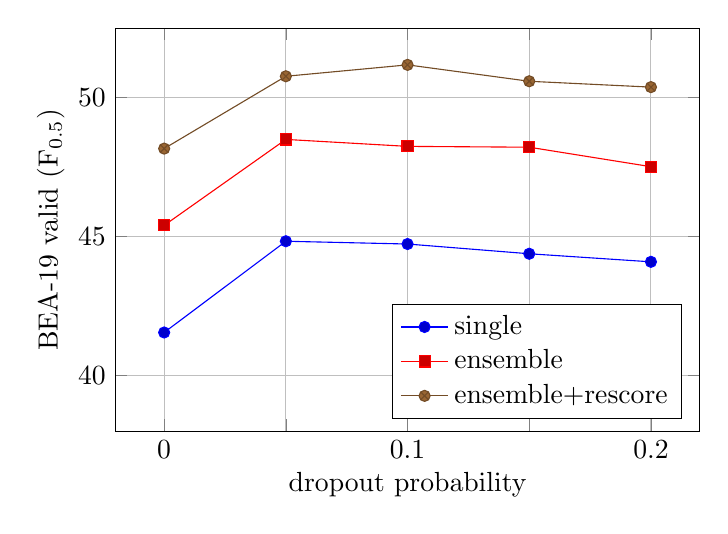
\begin{tikzpicture}
			\begin{axis}[
				ytick scale label code/.code={},
				ymin=38,
				xtick=data,
				height=6.7cm,
				xticklabels={0,,0.1,,0.2},
				width=9cm,
				grid=major,
				xlabel={dropout probability},
				ylabel={\text{BEA-19 valid} ($\text{F}_{0.5}$)},
				xlabel near ticks, xlabel shift={-2pt},
				ylabel near ticks, ylabel shift={-2pt},
				legend style={
					cells={anchor=west},
					legend pos=south east,
				}]
				\addplot coordinates {(0, 41.55) (0.05, 44.83) (0.1, 44.73)  (0.15, 44.38)  (0.2, 44.09)};
				\addplot coordinates {(0, 45.40) (0.05, 48.49) (0.1, 48.24)  (0.15, 48.21)  (0.2, 47.51)};
				\addplot coordinates {(0, 48.16) (0.05, 50.76) (0.1, 51.17)  (0.15, 50.58)  (0.2, 50.37)};
				\legend{\text{single}, \text{ensemble}, \text{ensemble+rescore}}
			\end{axis}
		\end{tikzpicture}
	\end{figure}
	\vspace{-2em}
	\begin{figure}[H]
		\centering
		\small
		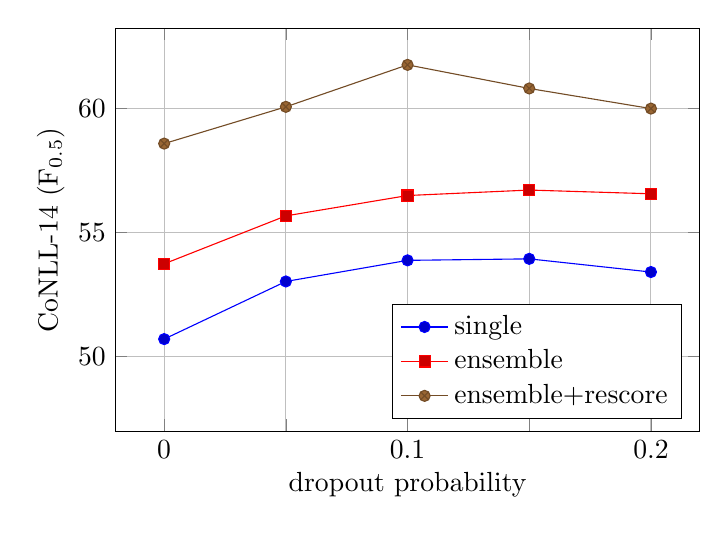
\begin{tikzpicture}
			\begin{axis}[
				ytick scale label code/.code={},
				ymin=47,
				xtick=data,
				height=6.7cm,
				xticklabels={0,,0.1,,0.2},
				width=9cm,
				grid=major,
				xlabel={dropout probability},
				ylabel={\text{CoNLL-14} ($\text{F}_{0.5}$)},
				xlabel near ticks, xlabel shift={-2pt},
				ylabel near ticks, ylabel shift={-2pt},
				legend style={
					cells={anchor=west},
					legend pos=south east,
				}]
				\addplot coordinates {(0, 50.71) (0.05, 53.03) (0.1, 53.88)  (0.15, 53.94)  (0.2, 53.41)};
				\addplot coordinates {(0, 53.74) (0.05, 55.67) (0.1, 56.49)  (0.15, 56.71)  (0.2, 56.56)};
				\addplot coordinates {(0, 58.58) (0.05, 60.06) (0.1, 61.75)  (0.15, 60.80)  (0.2, 59.99)};
				\legend{\text{single}, \text{ensemble}, \text{ensemble+rescore}}
			\end{axis}
		\end{tikzpicture}
	\end{figure}
	\vspace{-2em}
	\begin{figure}[H]
		\centering
		\small
		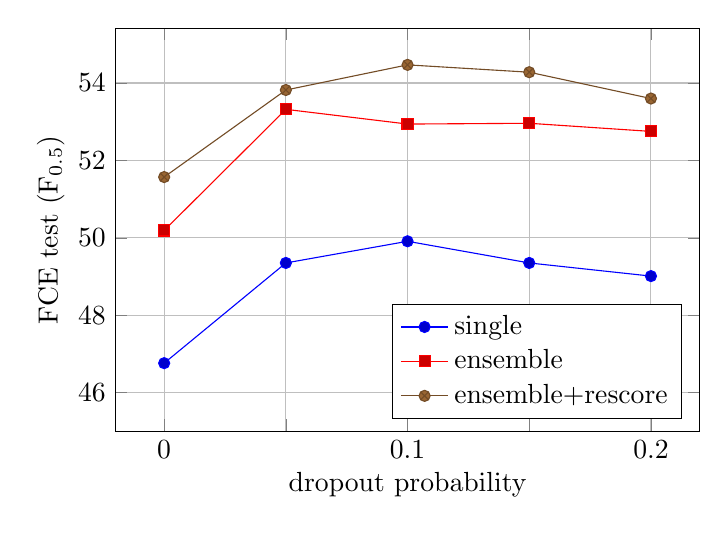
\begin{tikzpicture}
			\begin{axis}[
				ytick scale label code/.code={},
				ymin=45,
				xtick=data,
				height=6.7cm,
				xticklabels={0,,0.1,,0.2},
				width=9cm,
				grid=major,
				xlabel={dropout probability},
				ylabel={\text{FCE test} ($\text{F}_{0.5}$)},
				xlabel near ticks, xlabel shift={-2pt},
				ylabel near ticks, ylabel shift={-2pt},
				legend style={
					cells={anchor=west},
					legend pos=south east,
				}]
				\addplot coordinates {(0, 46.76) (0.05, 49.35) (0.1, 49.91)  (0.15, 49.35)  (0.2, 49.01)};
				\addplot coordinates {(0, 50.19) (0.05, 53.32) (0.1, 52.94)  (0.15, 52.96)  (0.2, 52.75)};
				\addplot coordinates {(0, 51.57) (0.05, 53.82) (0.1, 54.47)  (0.15, 54.28)  (0.2, 53.60)};
				\legend{\text{single}, \text{ensemble}, \text{ensemble+rescore}}
			\end{axis}
		\end{tikzpicture}
	\end{figure}
	\vspace{-2em}
	\begin{figure}[H]
		\centering
		\small
		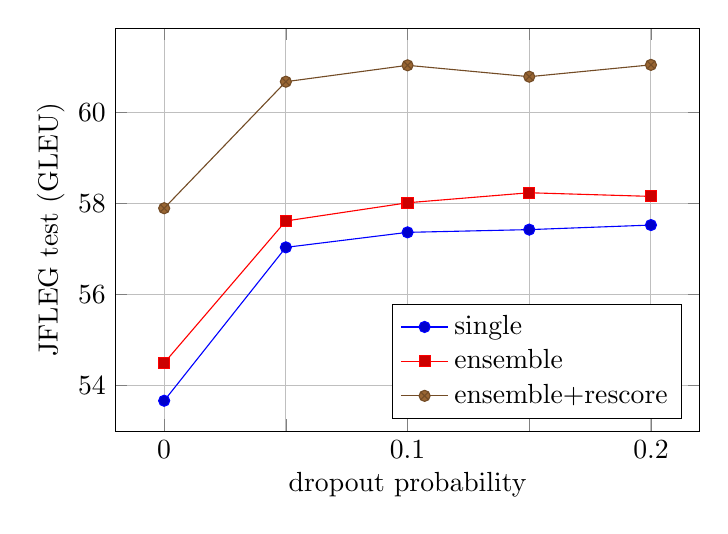
\begin{tikzpicture}
			\begin{axis}[
				ytick scale label code/.code={},
				ymin=53,
				xtick=data,
				height=6.7cm,
				xticklabels={0,,0.1,,0.2},
				width=9cm,
				grid=major,
				xlabel={dropout probability},
				ylabel={\text{JFLEG test} ($\text{GLEU}$)},
				xlabel near ticks, xlabel shift={-2pt},
				ylabel near ticks, ylabel shift={-2pt},
				legend style={
					cells={anchor=west},
					legend pos=south east,
				}]
				\addplot coordinates {(0, 53.67) (0.05, 57.04) (0.1, 57.37)  (0.15, 57.43)  (0.2, 57.53)};
				\addplot coordinates {(0, 54.50) (0.05, 57.62) (0.1, 58.02)  (0.15, 58.24)  (0.2, 58.16)};
				\addplot coordinates {(0, 57.90) (0.05, 60.68) (0.1, 61.04)  (0.15, 60.79)  (0.2, 61.05)};
				\legend{\text{single}, \text{ensemble}, \text{ensemble+rescore}}
			\end{axis}
		\end{tikzpicture}
	\end{figure}
	\vspace{-2em}
	\begin{figure}[H]
		\centering
		\small
		4M pre-training \\
		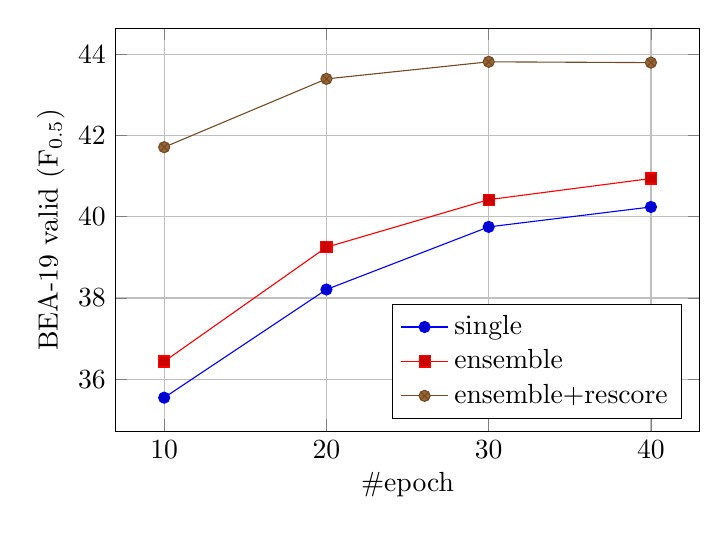
\begin{tikzpicture}
			\begin{axis}[
				ytick scale label code/.code={},
				%ymin=45,
				xtick=data,
				height=6.7cm,
				xticklabels={10,20,30,40},
				width=9cm,
				grid=major,
				xlabel={\#epoch},
				ylabel={BEA-19 valid ($\text{F}_{0.5}$)},
				xlabel near ticks, xlabel shift={-2pt},
				ylabel near ticks, ylabel shift={-2pt},
				legend style={
					cells={anchor=west},
					legend pos=south east,
				}]
				\addplot coordinates {(10, 35.55) (20, 38.21) (30, 39.75) (40, 40.24)};
				\addplot coordinates {(10, 36.44) (20, 39.25) (30, 40.42) (40, 40.94)};
				\addplot coordinates {(10, 41.71) (20, 43.39) (30, 43.81) (40, 43.79)};
				\legend{\text{single}, \text{ensemble}, \text{ensemble+rescore}}
			\end{axis}
		\end{tikzpicture}
	\end{figure}
	\vspace{-2em}
	\begin{figure}[H]
		\centering
		\small
		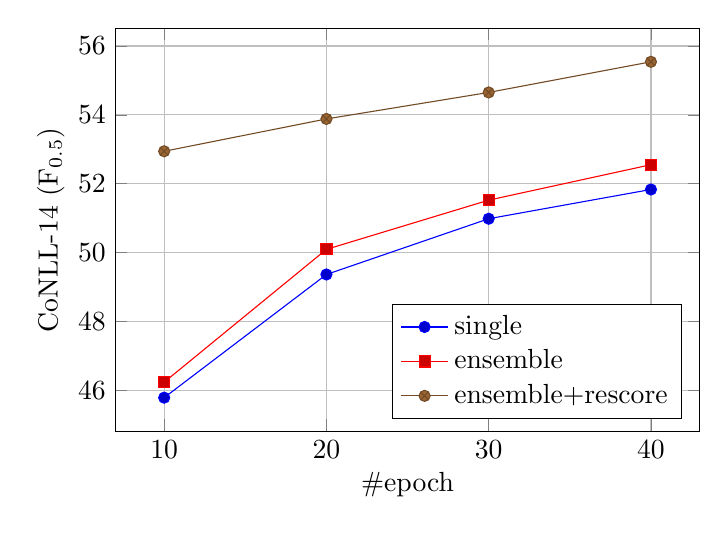
\begin{tikzpicture}
			\begin{axis}[
				ytick scale label code/.code={},
				%ymin=45,
				xtick=data,
				height=6.7cm,
				xticklabels={10,20,30,40},
				width=9cm,
				grid=major,
				xlabel={\#epoch},
				ylabel={CoNLL-14 ($\text{F}_{0.5}$)},
				xlabel near ticks, xlabel shift={-2pt},
				ylabel near ticks, ylabel shift={-2pt},
				legend style={
					cells={anchor=west},
					legend pos=south east,
				}]
				\addplot coordinates {(10, 45.78) (20, 49.36) (30, 50.98) (40, 51.83)};
				\addplot coordinates {(10, 46.23) (20, 50.09) (30, 51.52) (40, 52.55)};
				\addplot coordinates {(10, 52.94) (20, 53.88) (30, 54.65) (40, 55.54)};
				\legend{\text{single}, \text{ensemble}, \text{ensemble+rescore}}
			\end{axis}
		\end{tikzpicture}
	\end{figure}
	\vspace{-2em}
	\begin{figure}[H]
		\centering
		\small
		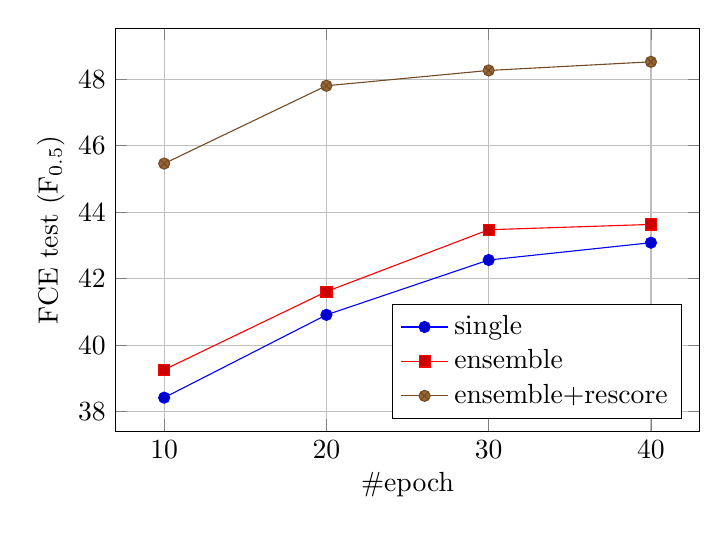
\begin{tikzpicture}
			\begin{axis}[
				ytick scale label code/.code={},
				%ymin=45,
				xtick=data,
				height=6.7cm,
				xticklabels={10,20,30,40},
				width=9cm,
				grid=major,
				xlabel={\#epoch},
				ylabel={FCE test ($\text{F}_{0.5}$)},
				xlabel near ticks, xlabel shift={-2pt},
				ylabel near ticks, ylabel shift={-2pt},
				legend style={
					cells={anchor=west},
					legend pos=south east,
				}]
				\addplot coordinates {(10, 38.42) (20, 40.91) (30, 42.56) (40, 43.08)};
				\addplot coordinates {(10, 39.26) (20, 41.61) (30, 43.47) (40, 43.63)};
				\addplot coordinates {(10, 45.46) (20, 47.80) (30, 48.26) (40, 48.52)};
				\legend{\text{single}, \text{ensemble}, \text{ensemble+rescore}}
			\end{axis}
		\end{tikzpicture}
	\end{figure}
	\vspace{-2em}
	\begin{figure}[H]
		\centering
		\small
		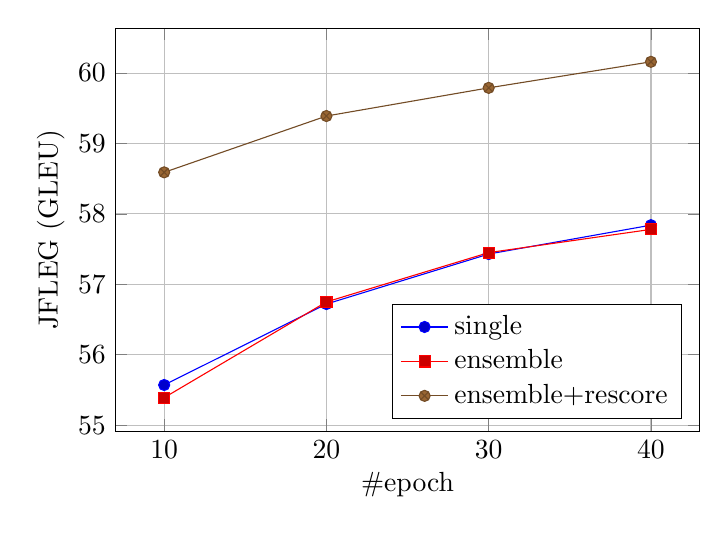
\begin{tikzpicture}
			\begin{axis}[
				ytick scale label code/.code={},
				%ymin=45,
				xtick=data,
				height=6.7cm,
				xticklabels={10,20,30,40},
				width=9cm,
				grid=major,
				xlabel={\#epoch},
				ylabel={JFLEG ($\text{GLEU}$)},
				xlabel near ticks, xlabel shift={-2pt},
				ylabel near ticks, ylabel shift={-2pt},
				legend style={
					cells={anchor=west},
					legend pos=south east,
				}]
				\addplot coordinates {(10, 55.57) (20, 56.72) (30, 57.43) (40, 57.84)};
				\addplot coordinates {(10, 55.39) (20, 56.75) (30, 57.45) (40, 57.78)};
				\addplot coordinates {(10, 58.59) (20, 59.39) (30, 59.79) (40, 60.16)};
				\legend{\text{single}, \text{ensemble}, \text{ensemble+rescore}}
			\end{axis}
		\end{tikzpicture}
	\end{figure}
	\vspace{-2em}
	\begin{figure}[H]
		\centering
		\small
		10 epochs pre-training \\
		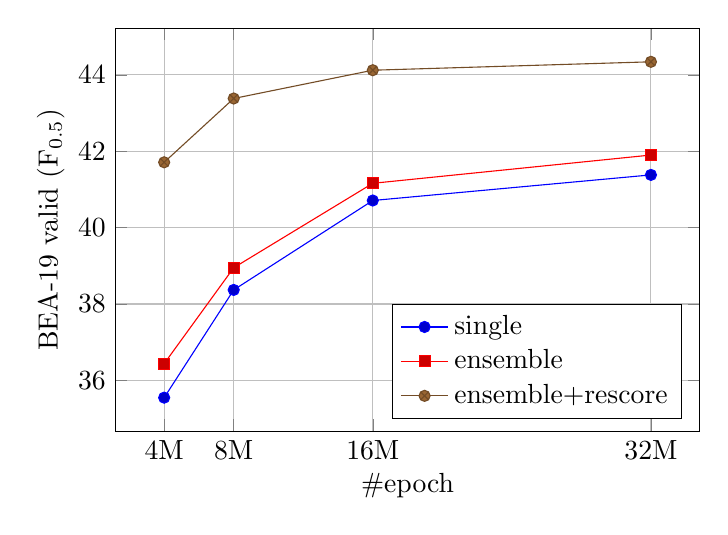
\begin{tikzpicture}
			\begin{axis}[
				ytick scale label code/.code={},
				%ymin=45,
				xtick=data,
				height=6.7cm,
				xticklabels={4M,8M,16M,32M},
				width=9cm,
				grid=major,
				xlabel={\#epoch},
				ylabel={BEA-19 valid ($\text{F}_{0.5}$)},
				xlabel near ticks, xlabel shift={-2pt},
				ylabel near ticks, ylabel shift={-2pt},
				legend style={
					cells={anchor=west},
					legend pos=south east,
				}]
				\addplot coordinates {(4, 35.55) (8, 38.37) (16, 40.71) (32, 41.38)};
				\addplot coordinates {(4, 36.44) (8, 38.95) (16, 41.16) (32, 41.90)};
				\addplot coordinates {(4, 41.71) (8, 43.38) (16, 44.12) (32, 44.34)};
				\legend{\text{single}, \text{ensemble}, \text{ensemble+rescore}}
			\end{axis}
		\end{tikzpicture}
	\end{figure}
	\vspace{-2em}
	\begin{figure}[H]
		\centering
		\small
		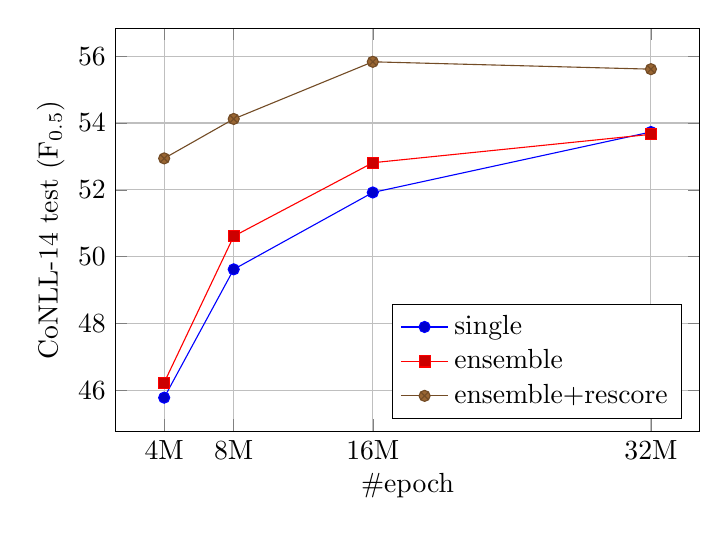
\begin{tikzpicture}
			\begin{axis}[
				ytick scale label code/.code={},
				%ymin=45,
				xtick=data,
				height=6.7cm,
				xticklabels={4M,8M,16M,32M},
				width=9cm,
				grid=major,
				xlabel={\#epoch},
				ylabel={CoNLL-14 test ($\text{F}_{0.5}$)},
				xlabel near ticks, xlabel shift={-2pt},
				ylabel near ticks, ylabel shift={-2pt},
				legend style={
					cells={anchor=west},
					legend pos=south east,
				}]
				\addplot coordinates {(4, 45.78) (8, 49.62) (16, 51.92) (32, 53.73)};
				\addplot coordinates {(4, 46.23) (8, 50.61) (16, 52.81) (32, 53.66)};
				\addplot coordinates {(4, 52.94) (8, 54.12) (16, 55.83) (32, 55.61)};
				\legend{\text{single}, \text{ensemble}, \text{ensemble+rescore}}
			\end{axis}
		\end{tikzpicture}
	\end{figure}
	\vspace{-2em}
	\begin{figure}[H]
		\centering
		\small
		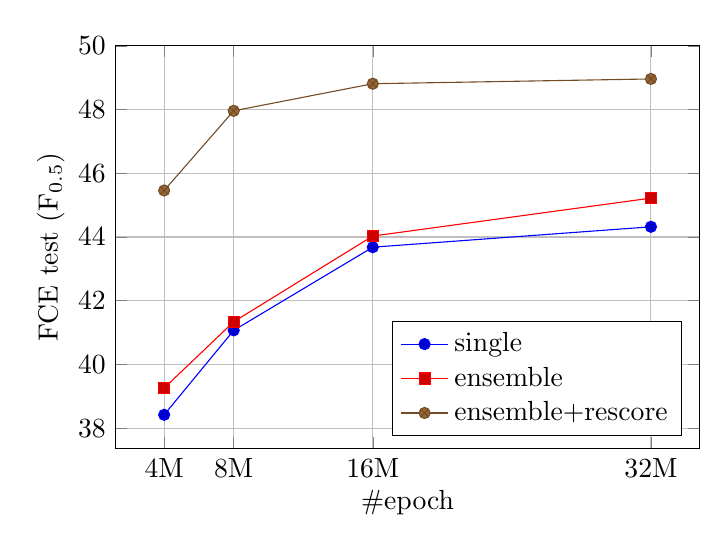
\begin{tikzpicture}
			\begin{axis}[
				ytick scale label code/.code={},
				%ymin=45,
				xtick=data,
				height=6.7cm,
				xticklabels={4M,8M,16M,32M},
				width=9cm,
				grid=major,
				xlabel={\#epoch},
				ylabel={FCE test ($\text{F}_{0.5}$)},
				xlabel near ticks, xlabel shift={-2pt},
				ylabel near ticks, ylabel shift={-2pt},
				legend style={
					cells={anchor=west},
					legend pos=south east,
				}]
				\addplot coordinates {(4, 38.42) (8, 41.07) (16, 43.68) (32, 44.32)};
				\addplot coordinates {(4, 39.26) (8, 41.34) (16, 44.03) (32, 45.22)};
				\addplot coordinates {(4, 45.46) (8, 47.96) (16, 48.81) (32, 48.96)};
				\legend{\text{single}, \text{ensemble}, \text{ensemble+rescore}}
			\end{axis}
		\end{tikzpicture}
	\end{figure}
	\vspace{-2em}
	\begin{figure}[H]
		\centering
		\small
		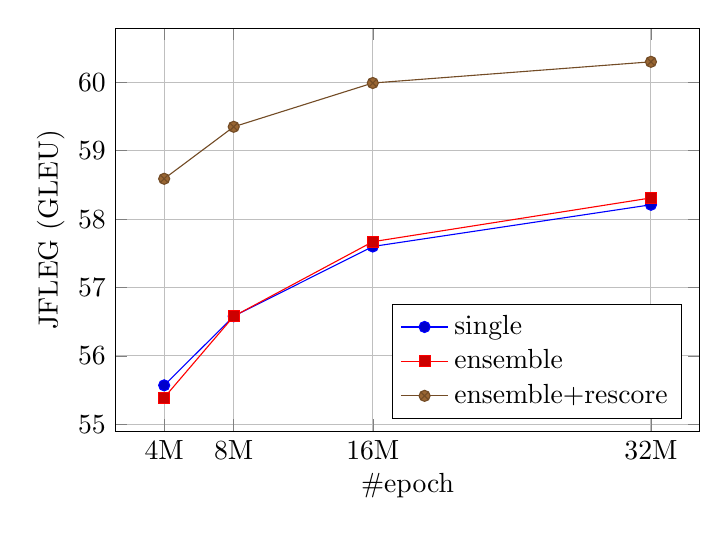
\begin{tikzpicture}
			\begin{axis}[
				ytick scale label code/.code={},
				%ymin=45,
				xtick=data,
				height=6.7cm,
				xticklabels={4M,8M,16M,32M},
				width=9cm,
				grid=major,
				xlabel={\#epoch},
				ylabel={JFLEG ($\text{GLEU}$)},
				xlabel near ticks, xlabel shift={-2pt},
				ylabel near ticks, ylabel shift={-2pt},
				legend style={
					cells={anchor=west},
					legend pos=south east,
				}]
				\addplot coordinates {(4, 55.57) (8, 56.58) (16, 57.60) (32, 58.21)};
				\addplot coordinates {(4, 55.39) (8, 56.58) (16, 57.67) (32, 58.31)};
				\addplot coordinates {(4, 58.59) (8, 59.35) (16, 59.99) (32, 60.30)};
				\legend{\text{single}, \text{ensemble}, \text{ensemble+rescore}}
			\end{axis}
		\end{tikzpicture}
	\end{figure}
	\vspace{-2em}
	\begin{figure}[H]
		\centering
		\small
		10 epochs pre-training + fine-tuning \\
		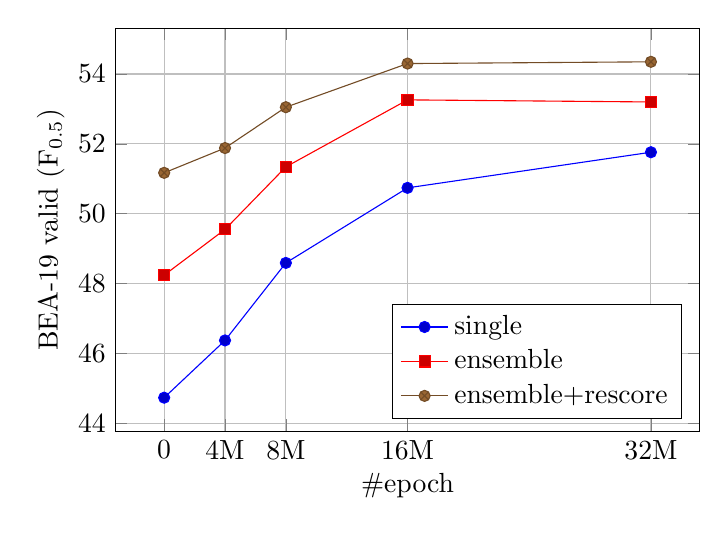
\begin{tikzpicture}
			\begin{axis}[
				ytick scale label code/.code={},
				%ymin=45,
				xtick=data,
				height=6.7cm,
				xticklabels={0,4M,8M,16M,32M},
				width=9cm,
				grid=major,
				xlabel={\#epoch},
				ylabel={BEA-19 valid ($\text{F}_{0.5}$)},
				xlabel near ticks, xlabel shift={-2pt},
				ylabel near ticks, ylabel shift={-2pt},
				legend style={
					cells={anchor=west},
					legend pos=south east,
				}]
				\addplot coordinates {(0, 44.73) (4, 46.37) (8, 48.59) (16, 50.74) (32, 51.76)};
				\addplot coordinates {(0, 48.24) (4, 49.55) (8, 51.34) (16, 53.26) (32, 53.20)};
				\addplot coordinates {(0, 51.17) (4, 51.88) (8, 53.05) (16, 54.30) (32, 54.35)};
				\legend{\text{single}, \text{ensemble}, \text{ensemble+rescore}}
			\end{axis}
		\end{tikzpicture}
	\end{figure}
	\vspace{-2em}
	\begin{figure}[H]
		\centering
		\small
		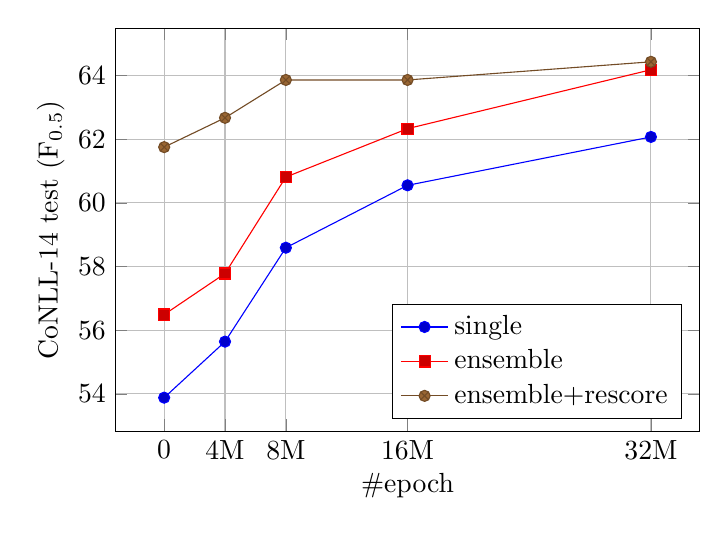
\begin{tikzpicture}
			\begin{axis}[
				ytick scale label code/.code={},
				%ymin=45,
				xtick=data,
				height=6.7cm,
				xticklabels={0,4M,8M,16M,32M},
				width=9cm,
				grid=major,
				xlabel={\#epoch},
				ylabel={CoNLL-14 test ($\text{F}_{0.5}$)},
				xlabel near ticks, xlabel shift={-2pt},
				ylabel near ticks, ylabel shift={-2pt},
				legend style={
					cells={anchor=west},
					legend pos=south east,
				}]
				\addplot coordinates {(0, 53.88) (4, 55.64) (8, 58.59) (16, 60.55) (32, 62.07)};
				\addplot coordinates {(0, 56.49) (4, 57.78) (8, 60.81) (16, 62.33) (32, 64.18)};
				\addplot coordinates {(0, 61.75) (4, 62.67) (8, 63.86) (16, 63.86) (32, 64.43)};
				\legend{\text{single}, \text{ensemble}, \text{ensemble+rescore}}
			\end{axis}
		\end{tikzpicture}
	\end{figure}
	\vspace{-2em}
	\begin{figure}[H]
		\centering
		\small
		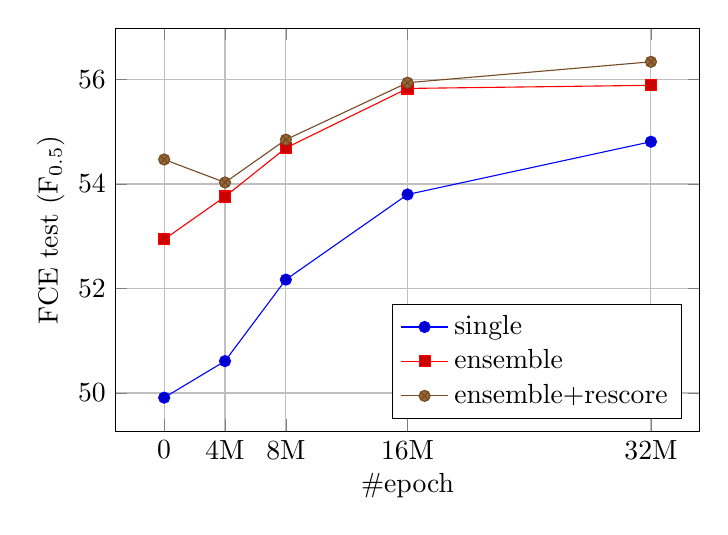
\begin{tikzpicture}
			\begin{axis}[
				ytick scale label code/.code={},
				%ymin=45,
				xtick=data,
				height=6.7cm,
				xticklabels={0,4M,8M,16M,32M},
				width=9cm,
				grid=major,
				xlabel={\#epoch},
				ylabel={FCE test ($\text{F}_{0.5}$)},
				xlabel near ticks, xlabel shift={-2pt},
				ylabel near ticks, ylabel shift={-2pt},
				legend style={
					cells={anchor=west},
					legend pos=south east,
				}]
				\addplot coordinates {(0, 49.91) (4, 50.61) (8, 52.17) (16, 53.80) (32, 54.81)};
				\addplot coordinates {(0, 52.94) (4, 53.76) (8, 54.69) (16, 55.83) (32, 55.89)};
				\addplot coordinates {(0, 54.47) (4, 54.03) (8, 54.85) (16, 55.94) (32, 56.34)};
				\legend{\text{single}, \text{ensemble}, \text{ensemble+rescore}}
			\end{axis}
		\end{tikzpicture}
	\end{figure}
	\vspace{-2em}
	\begin{figure}[H]
		\centering
		\small
		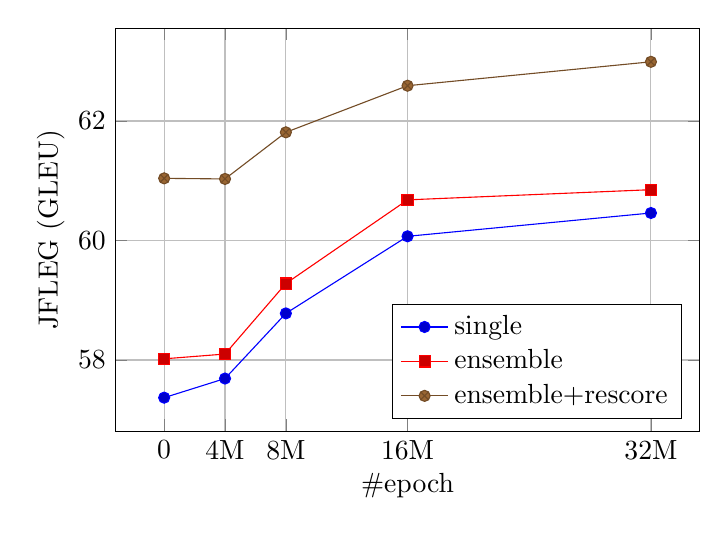
\begin{tikzpicture}
			\begin{axis}[
				ytick scale label code/.code={},
				%ymin=45,
				xtick=data,
				height=6.7cm,
				xticklabels={0,4M,8M,16M,32M},
				width=9cm,
				grid=major,
				xlabel={\#epoch},
				ylabel={JFLEG ($\text{GLEU}$)},
				xlabel near ticks, xlabel shift={-2pt},
				ylabel near ticks, ylabel shift={-2pt},
				legend style={
					cells={anchor=west},
					legend pos=south east,
				}]
				\addplot coordinates {(0, 57.37) (4, 57.69) (8, 58.78) (16, 60.07) (32, 60.46)};
				\addplot coordinates {(0, 58.02) (4, 58.10) (8, 59.28) (16, 60.68) (32, 60.85)};
				\addplot coordinates {(0, 61.04) (4, 61.03) (8, 61.81) (16, 62.59) (32, 62.99)};
				\legend{\text{single}, \text{ensemble}, \text{ensemble+rescore}}
			\end{axis}
		\end{tikzpicture}
	\end{figure}
	\vspace{-2em}
	\begin{figure}[H]
		\centering
		\small
		pre-training with fixed \#step \\
		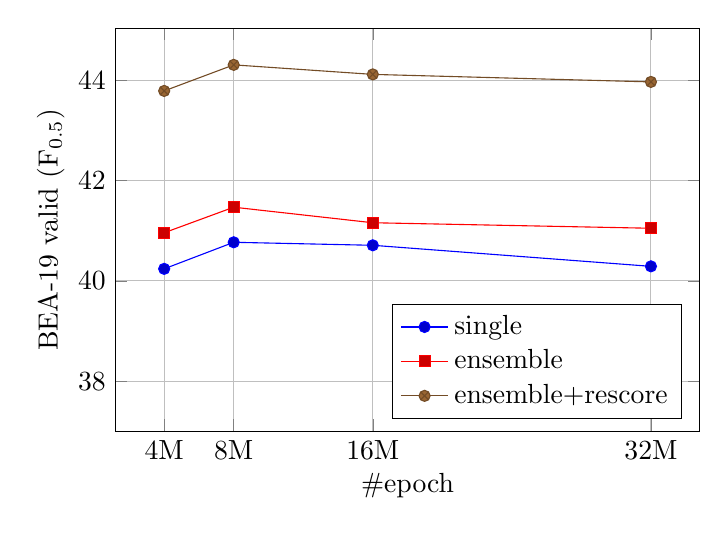
\begin{tikzpicture}
			\begin{axis}[
				ytick scale label code/.code={},
				ymin=37,
				xtick=data,
				height=6.7cm,
				xticklabels={4M,8M,16M,32M},
				width=9cm,
				grid=major,
				xlabel={\#epoch},
				ylabel={BEA-19 valid ($\text{F}_{0.5}$)},
				xlabel near ticks, xlabel shift={-2pt},
				ylabel near ticks, ylabel shift={-2pt},
				legend style={
					cells={anchor=west},
					legend pos=south east,
				}]
				\addplot coordinates {(4, 40.24) (8, 40.77) (16, 40.71) (32, 40.29)};
				\addplot coordinates {(4, 40.96) (8, 41.47) (16, 41.16) (32, 41.05)};
				\addplot coordinates {(4, 43.79) (8, 44.31) (16, 44.12) (32, 43.97)};
				\legend{\text{single}, \text{ensemble}, \text{ensemble+rescore}}
			\end{axis}
		\end{tikzpicture}
	\end{figure}
	\vspace{-2em}
	\begin{figure}[H]
		\centering
		\small
		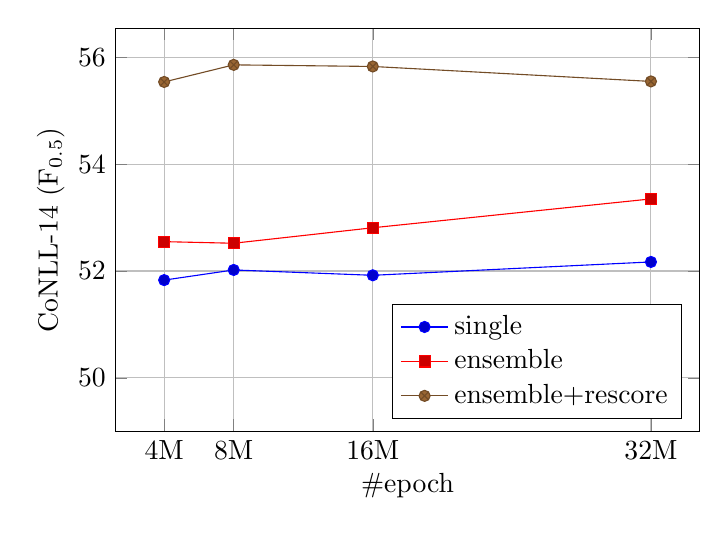
\begin{tikzpicture}
			\begin{axis}[
				ytick scale label code/.code={},
				ymin=49,
				xtick=data,
				height=6.7cm,
				xticklabels={4M,8M,16M,32M},
				width=9cm,
				grid=major,
				xlabel={\#epoch},
				ylabel={CoNLL-14 ($\text{F}_{0.5}$)},
				xlabel near ticks, xlabel shift={-2pt},
				ylabel near ticks, ylabel shift={-2pt},
				legend style={
					cells={anchor=west},
					legend pos=south east,
				}]
				\addplot coordinates {(4, 51.83) (8, 52.02) (16, 51.92) (32, 52.17)};
				\addplot coordinates {(4, 52.55) (8, 52.52) (16, 52.81) (32, 53.35)};
				\addplot coordinates {(4, 55.54) (8, 55.86) (16, 55.83) (32, 55.55)};
				\legend{\text{single}, \text{ensemble}, \text{ensemble+rescore}}
			\end{axis}
		\end{tikzpicture}
	\end{figure}
	\vspace{-2em}
	\begin{figure}[H]
		\centering
		\small
		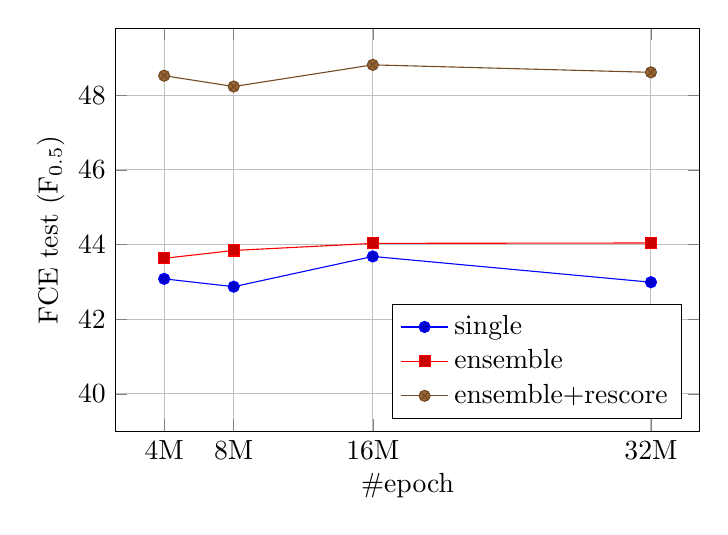
\begin{tikzpicture}
			\begin{axis}[
				ytick scale label code/.code={},
				ymin=39,
				xtick=data,
				height=6.7cm,
				xticklabels={4M,8M,16M,32M},
				width=9cm,
				grid=major,
				xlabel={\#epoch},
				ylabel={FCE test ($\text{F}_{0.5}$)},
				xlabel near ticks, xlabel shift={-2pt},
				ylabel near ticks, ylabel shift={-2pt},
				legend style={
					cells={anchor=west},
					legend pos=south east,
				}]
				\addplot coordinates {(4, 43.08) (8, 42.87) (16, 43.68) (32, 42.99)};
				\addplot coordinates {(4, 43.63) (8, 43.84) (16, 44.03) (32, 44.04)};
				\addplot coordinates {(4, 48.52) (8, 48.23) (16, 48.81) (32, 48.61)};
				\legend{\text{single}, \text{ensemble}, \text{ensemble+rescore}}
			\end{axis}
		\end{tikzpicture}
	\end{figure}
	\vspace{-2em}
	\begin{figure}[H]
		\centering
		\small
		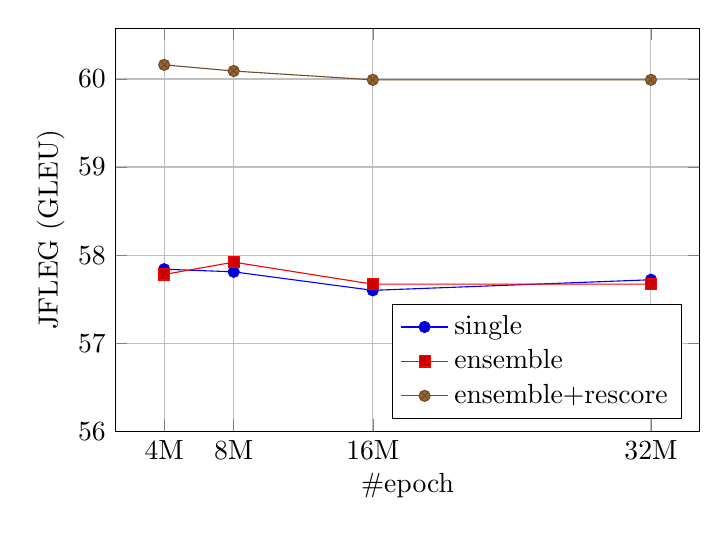
\begin{tikzpicture}
			\begin{axis}[
				ytick scale label code/.code={},
				ymin=56,
				xtick=data,
				height=6.7cm,
				xticklabels={4M,8M,16M,32M},
				width=9cm,
				grid=major,
				xlabel={\#epoch},
				ylabel={JFLEG ($\text{GLEU}$)},
				xlabel near ticks, xlabel shift={-2pt},
				ylabel near ticks, ylabel shift={-2pt},
				legend style={
					cells={anchor=west},
					legend pos=south east,
				}]
				\addplot coordinates {(4, 57.84) (8, 57.81) (16, 57.60) (32, 57.72)};
				\addplot coordinates {(4, 57.78) (8, 57.92) (16, 57.67) (32, 57.67)};
				\addplot coordinates {(4, 60.16) (8, 60.09) (16, 59.99) (32, 59.99)};
				\legend{\text{single}, \text{ensemble}, \text{ensemble+rescore}}
			\end{axis}
		\end{tikzpicture}
	\end{figure}
	\vspace{-2em}
	\begin{figure}[H]
		\centering
		\small
		pre-training with fixed \#step + fine-tuning \\
		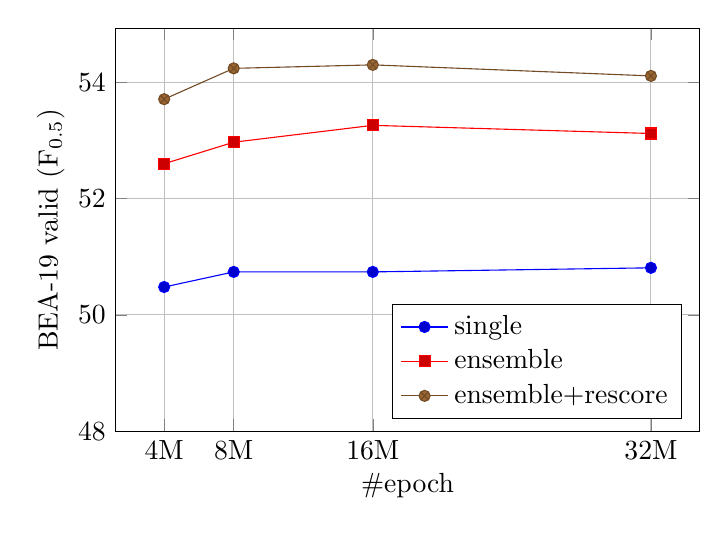
\begin{tikzpicture}
			\begin{axis}[
				ytick scale label code/.code={},
				ymin=48,
				xtick=data,
				height=6.7cm,
				xticklabels={4M,8M,16M,32M},
				width=9cm,
				grid=major,
				xlabel={\#epoch},
				ylabel={BEA-19 valid ($\text{F}_{0.5}$)},
				xlabel near ticks, xlabel shift={-2pt},
				ylabel near ticks, ylabel shift={-2pt},
				legend style={
					cells={anchor=west},
					legend pos=south east,
				}]
				\addplot coordinates {(4, 50.48) (8, 50.74) (16, 50.74) (32, 50.81)};
				\addplot coordinates {(4, 52.60) (8, 52.97) (16, 53.26) (32, 53.12)};
				\addplot coordinates {(4, 53.71) (8, 54.24) (16, 54.30) (32, 54.11)};
				\legend{\text{single}, \text{ensemble}, \text{ensemble+rescore}}
			\end{axis}
		\end{tikzpicture}
	\end{figure}
	\vspace{-2em}
	\begin{figure}[H]
		\centering
		\small
		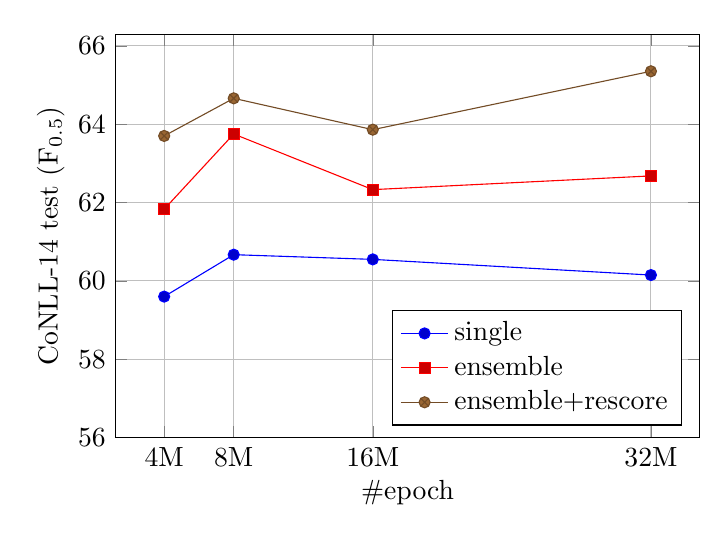
\begin{tikzpicture}
			\begin{axis}[
				ytick scale label code/.code={},
				ymin=56,
				xtick=data,
				height=6.7cm,
				xticklabels={4M,8M,16M,32M},
				width=9cm,
				grid=major,
				xlabel={\#epoch},
				ylabel={CoNLL-14 test ($\text{F}_{0.5}$)},
				xlabel near ticks, xlabel shift={-2pt},
				ylabel near ticks, ylabel shift={-2pt},
				legend style={
					cells={anchor=west},
					legend pos=south east,
				}]
				\addplot coordinates {(4, 59.60) (8, 60.67) (16, 60.55) (32, 60.15)};
				\addplot coordinates {(4, 61.83) (8, 63.75) (16, 62.33) (32, 62.68)};
				\addplot coordinates {(4, 63.70) (8, 64.66) (16, 63.86) (32, 65.35)};
				\legend{\text{single}, \text{ensemble}, \text{ensemble+rescore}}
			\end{axis}
		\end{tikzpicture}
	\end{figure}
	\vspace{-2em}
	\begin{figure}[H]
		\centering
		\small
		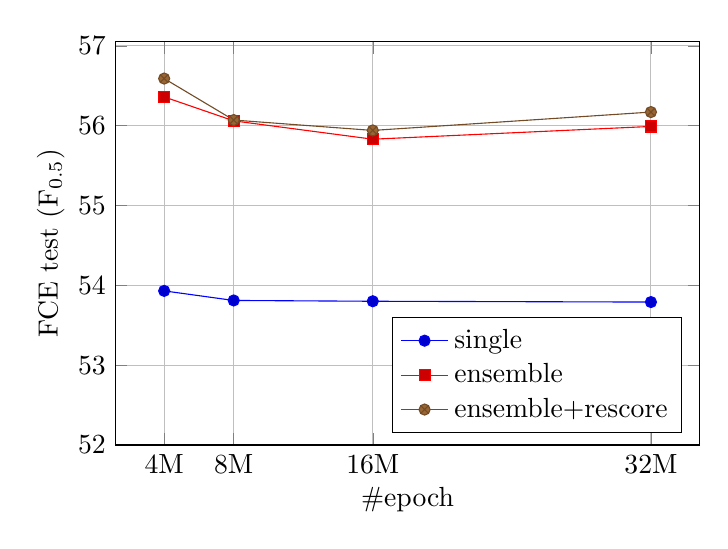
\begin{tikzpicture}
			\begin{axis}[
				ytick scale label code/.code={},
				ymin=52,
				xtick=data,
				height=6.7cm,
				xticklabels={4M,8M,16M,32M},
				width=9cm,
				grid=major,
				xlabel={\#epoch},
				ylabel={FCE test ($\text{F}_{0.5}$)},
				xlabel near ticks, xlabel shift={-2pt},
				ylabel near ticks, ylabel shift={-2pt},
				legend style={
					cells={anchor=west},
					legend pos=south east,
				}]
				\addplot coordinates {(4, 53.93) (8, 53.81) (16, 53.80) (32, 53.79)};
				\addplot coordinates {(4, 56.36) (8, 56.06) (16, 55.83) (32, 55.99)};
				\addplot coordinates {(4, 56.59) (8, 56.07) (16, 55.94) (32, 56.17)};
				\legend{\text{single}, \text{ensemble}, \text{ensemble+rescore}}
			\end{axis}
		\end{tikzpicture}
	\end{figure}
	\vspace{-2em}
	\begin{figure}[H]
		\centering
		\small
		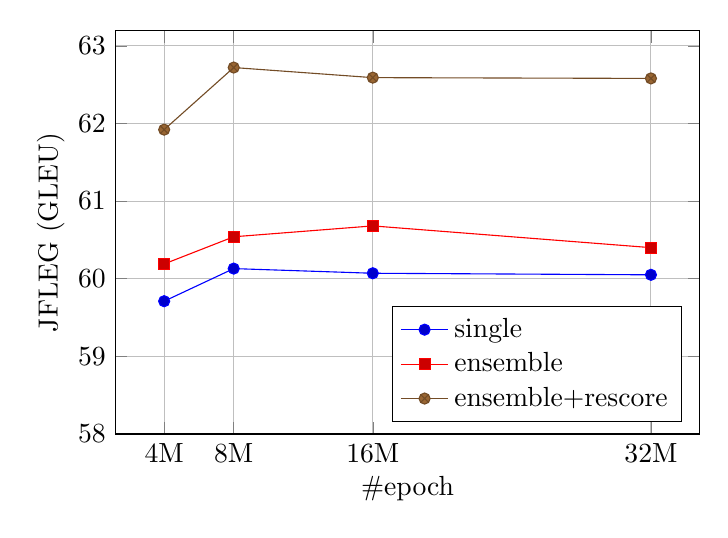
\begin{tikzpicture}
			\begin{axis}[
				ytick scale label code/.code={},
				ymin=58,
				xtick=data,
				height=6.7cm,
				xticklabels={4M,8M,16M,32M},
				width=9cm,
				grid=major,
				xlabel={\#epoch},
				ylabel={JFLEG ($\text{GLEU}$)},
				xlabel near ticks, xlabel shift={-2pt},
				ylabel near ticks, ylabel shift={-2pt},
				legend style={
					cells={anchor=west},
					legend pos=south east,
				}]
				\addplot coordinates {(4, 59.71) (8, 60.13) (16, 60.07) (32, 60.05)};
				\addplot coordinates {(4, 60.19) (8, 60.54) (16, 60.68) (32, 60.40)};
				\addplot coordinates {(4, 61.92) (8, 62.72) (16, 62.59) (32, 62.58)};
				\legend{\text{single}, \text{ensemble}, \text{ensemble+rescore}}
			\end{axis}
		\end{tikzpicture}
	\end{figure}
	\vspace{-2em}
\end{multicols*}

\begin{figure}[H]
	\centering
	\small
	8M x 10 epochs pre-training + fine-tuning
	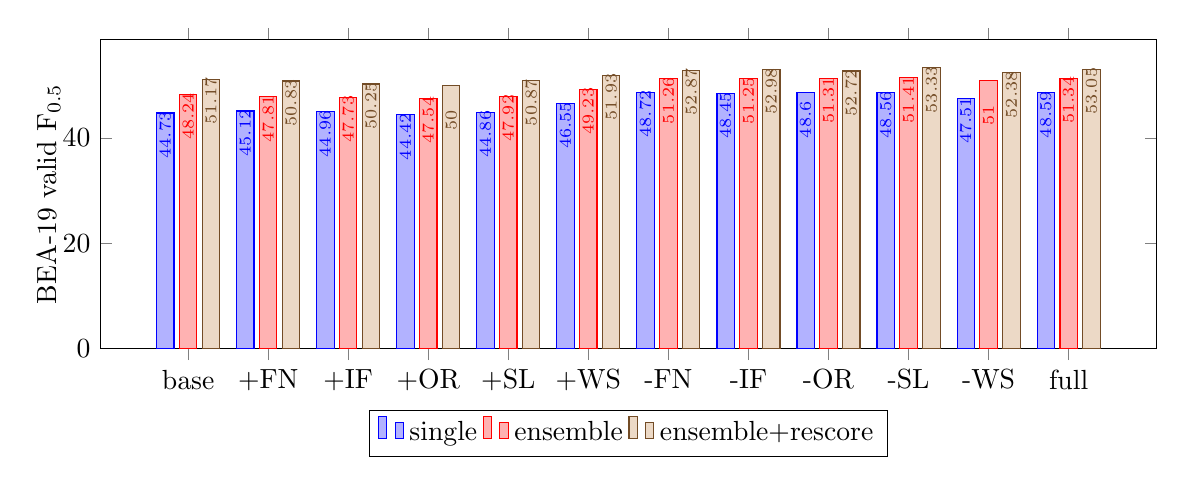
\begin{tikzpicture}
		\begin{axis}[
				ybar,
				ymin=0,
				%ymax=100,
				width=15cm,
				height=5.5cm,
				xlabel near ticks, xlabel shift={-2pt},
				ylabel near ticks, ylabel shift={-6pt},
				bar width=0.22cm,
				%enlargelimits=0.15,
				legend style={at={(0.5,-0.20)},
				anchor=north,legend columns=-1},
				ylabel={BEA-19 valid F${}_{0.5}$},
				symbolic x coords={base, +FN, +IF, +OR, +SL, +WS, -FN, -IF, -OR, -SL, -WS, full},
				xtick=data,
				nodes near coords,
				every node near coord/.append style={rotate=90, anchor=west, xshift=-0.7cm, font=\fontsize{6.5pt}{0.5pt}\selectfont},
			]
			\addplot coordinates {(base, 44.73) (+FN, 45.12) (+IF, 44.96) (+OR, 44.42) (+SL, 44.86) (+WS, 46.55) (-FN, 48.72) (-IF, 48.45) (-OR, 48.60) (-SL, 48.56) (-WS, 47.51) (full, 48.59)};
			\addplot coordinates {(base, 48.24) (+FN, 47.81) (+IF, 47.73) (+OR, 47.54) (+SL, 47.92) (+WS, 49.23) (-FN, 51.26) (-IF, 51.25) (-OR, 51.31) (-SL, 51.41) (-WS, 51.00) (full, 51.34)};
			\addplot coordinates {(base, 51.17) (+FN, 50.83) (+IF, 50.25) (+OR, 50.00) (+SL, 50.87) (+WS, 51.93) (-FN, 52.87) (-IF, 52.98) (-OR, 52.72) (-SL, 53.33) (-WS, 52.38) (full, 53.05)};
			\legend{single, ensemble, ensemble+rescore}
		\end{axis}
	\end{tikzpicture}
\end{figure}

\begin{figure}[H]
	\centering
	\small
	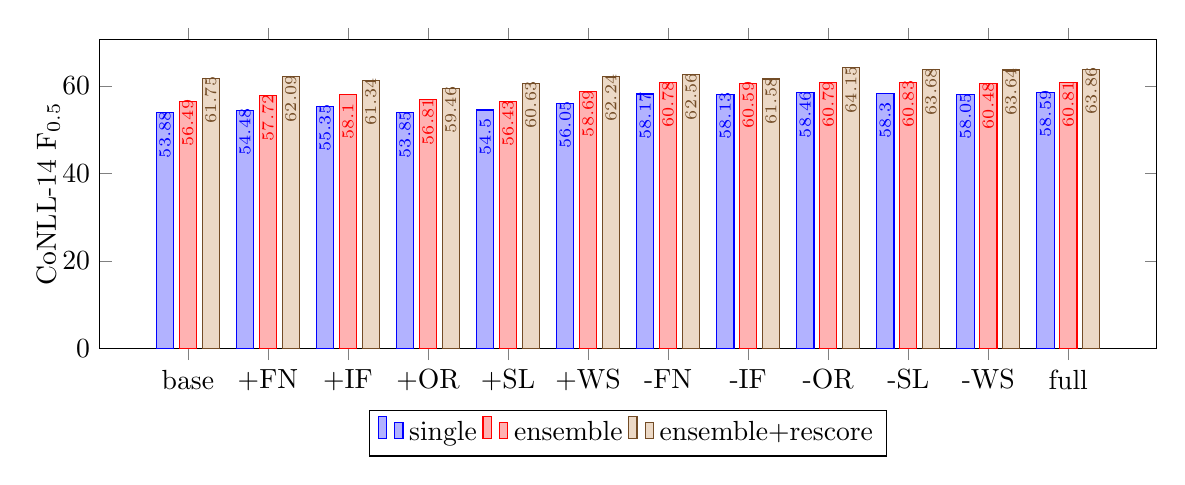
\begin{tikzpicture}
		\begin{axis}[
				ybar,
				ymin=0,
				%ymax=100,
				width=15cm,
				height=5.5cm,
				xlabel near ticks, xlabel shift={-2pt},
				ylabel near ticks, ylabel shift={-6pt},
				bar width=0.22cm,
				%enlargelimits=0.15,
				legend style={at={(0.5,-0.20)},
				anchor=north,legend columns=-1},
				ylabel={CoNLL-14 F${}_{0.5}$},
				symbolic x coords={base, +FN, +IF, +OR, +SL, +WS, -FN, -IF, -OR, -SL, -WS, full},
				xtick=data,
				nodes near coords,
				every node near coord/.append style={rotate=90, anchor=west, xshift=-0.7cm, font=\fontsize{6.5pt}{0.5pt}\selectfont},
			]
			\addplot coordinates {(base, 53.88) (+FN, 54.48) (+IF, 55.35) (+OR, 53.85) (+SL, 54.50) (+WS, 56.05) (-FN, 58.17) (-IF, 58.13) (-OR, 58.46) (-SL, 58.30) (-WS, 58.05) (full, 58.59)};
			\addplot coordinates {(base, 56.49) (+FN, 57.72) (+IF, 58.10) (+OR, 56.81) (+SL, 56.43) (+WS, 58.69) (-FN, 60.78) (-IF, 60.59) (-OR, 60.79) (-SL, 60.83) (-WS, 60.48) (full, 60.81)};
			\addplot coordinates {(base, 61.75) (+FN, 62.09) (+IF, 61.34) (+OR, 59.46) (+SL, 60.63) (+WS, 62.24) (-FN, 62.56) (-IF, 61.58) (-OR, 64.15) (-SL, 63.68) (-WS, 63.64) (full, 63.86)};
			\legend{single, ensemble, ensemble+rescore}
		\end{axis}
	\end{tikzpicture}
\end{figure}

\begin{figure}[H]
	\centering
	\small
	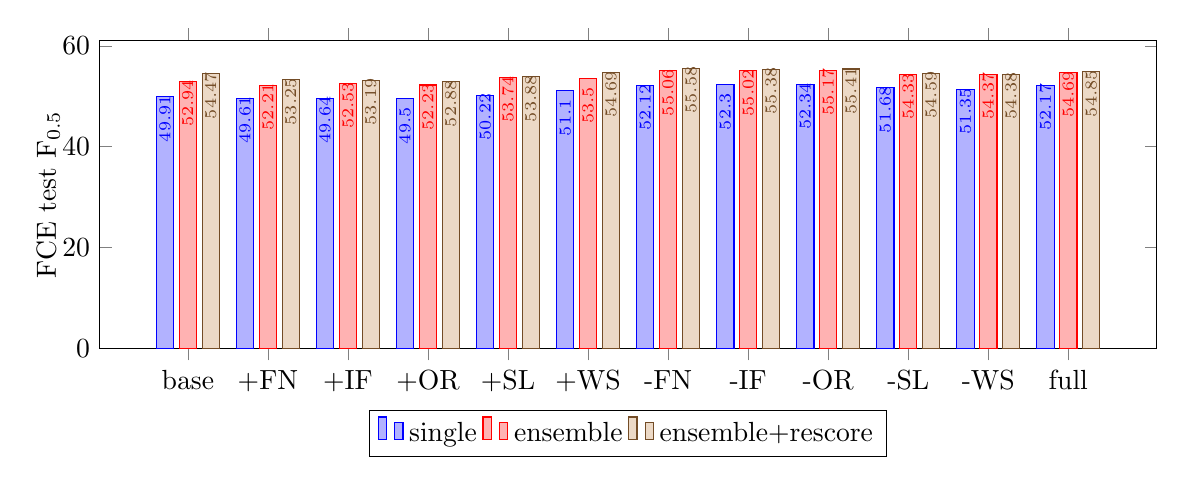
\begin{tikzpicture}
		\begin{axis}[
				ybar,
				ymin=0,
				%ymax=100,
				width=15cm,
				height=5.5cm,
				xlabel near ticks, xlabel shift={-2pt},
				ylabel near ticks, ylabel shift={-6pt},
				bar width=0.22cm,
				%enlargelimits=0.15,
				legend style={at={(0.5,-0.20)},
				anchor=north,legend columns=-1},
				ylabel={FCE test F${}_{0.5}$},
				symbolic x coords={base, +FN, +IF, +OR, +SL, +WS, -FN, -IF, -OR, -SL, -WS, full},
				xtick=data,
				nodes near coords,
				every node near coord/.append style={rotate=90, anchor=west, xshift=-0.7cm, font=\fontsize{6.5pt}{0.5pt}\selectfont},
			]
			\addplot coordinates {(base, 49.91) (+FN, 49.61) (+IF, 49.64) (+OR, 49.50) (+SL, 50.22) (+WS, 51.10) (-FN, 52.12) (-IF, 52.30) (-OR, 52.34) (-SL, 51.68) (-WS, 51.35) (full, 52.17)};
			\addplot coordinates {(base, 52.94) (+FN, 52.21) (+IF, 52.53) (+OR, 52.23) (+SL, 53.74) (+WS, 53.50) (-FN, 55.06) (-IF, 55.02) (-OR, 55.17) (-SL, 54.33) (-WS, 54.37) (full, 54.69)};
			\addplot coordinates {(base, 54.47) (+FN, 53.25) (+IF, 53.19) (+OR, 52.88) (+SL, 53.88) (+WS, 54.69) (-FN, 55.58) (-IF, 55.38) (-OR, 55.41) (-SL, 54.59) (-WS, 54.38) (full, 54.85)};
			\legend{single, ensemble, ensemble+rescore}
		\end{axis}
	\end{tikzpicture}
\end{figure}

\begin{figure}[H]
	\centering
	\small
	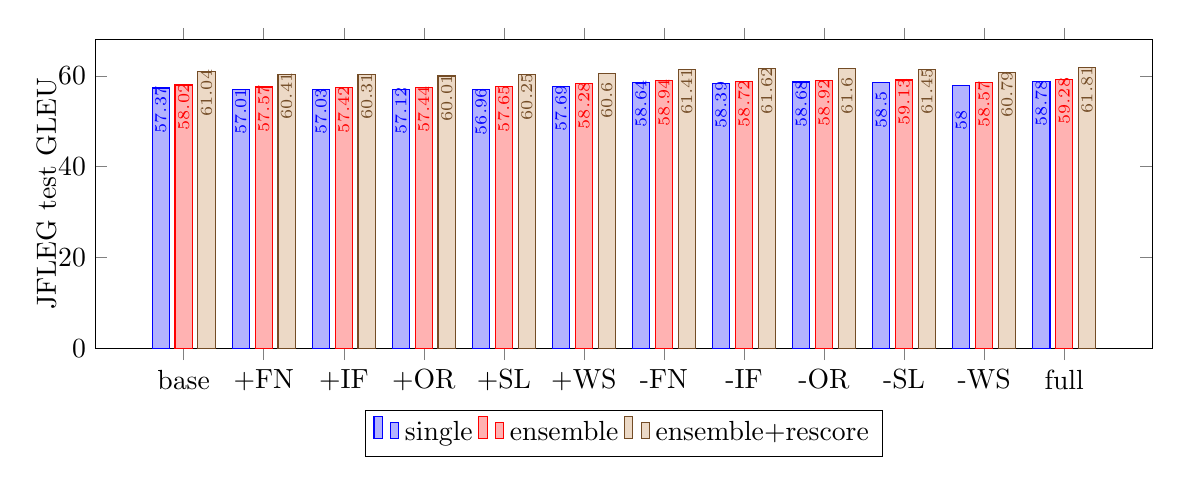
\begin{tikzpicture}
		\begin{axis}[
				ybar,
				ymin=0,
				%ymax=100,
				width=15cm,
				height=5.5cm,
				xlabel near ticks, xlabel shift={-2pt},
				ylabel near ticks, ylabel shift={-6pt},
				bar width=0.22cm,
				%enlargelimits=0.15,
				legend style={at={(0.5,-0.20)},
				anchor=north,legend columns=-1},
				ylabel={JFLEG test GLEU},
				symbolic x coords={base, +FN, +IF, +OR, +SL, +WS, -FN, -IF, -OR, -SL, -WS, full},
				xtick=data,
				nodes near coords,
				every node near coord/.append style={rotate=90, anchor=west, xshift=-0.7cm, font=\fontsize{6.5pt}{0.5pt}\selectfont},
			]
			\addplot coordinates {(base, 57.37) (+FN, 57.01) (+IF, 57.03) (+OR, 57.12) (+SL, 56.96) (+WS, 57.69) (-FN, 58.64) (-IF, 58.39) (-OR, 58.68) (-SL, 58.50) (-WS, 58.00) (full, 58.78)};
			\addplot coordinates {(base, 58.02) (+FN, 57.57) (+IF, 57.42) (+OR, 57.44) (+SL, 57.65) (+WS, 58.28) (-FN, 58.94) (-IF, 58.72) (-OR, 58.92) (-SL, 59.13) (-WS, 58.57) (full, 59.28)};
			\addplot coordinates {(base, 61.04) (+FN, 60.41) (+IF, 60.31) (+OR, 60.01) (+SL, 60.25) (+WS, 60.60) (-FN, 61.41) (-IF, 61.62) (-OR, 61.60) (-SL, 61.45) (-WS, 60.79) (full, 61.81)};
			\legend{single, ensemble, ensemble+rescore}
		\end{axis}
	\end{tikzpicture}
\end{figure}

\newpage

\begin{multicols}{2}
	\begin{figure}[H]
		\centering
		\small
		8M x 10 epochs pre-training + fine-tuning (ensemble) \\
		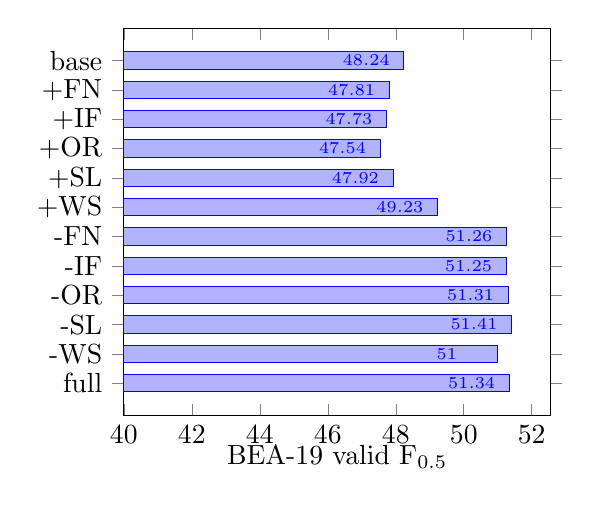
\begin{tikzpicture}
			\begin{axis}[
					xbar,
					xmin=40,
					%ymax=100,
					width=7cm,
					height=6.5cm,
					xlabel near ticks, xlabel shift={-6pt},
					ylabel near ticks, ylabel shift={-2pt},
					bar width=0.22cm,
					%enlargelimits=0.15,
					legend style={at={(0.5,-0.20)},
					anchor=north,legend columns=-1},
					xlabel={BEA-19 valid F${}_{0.5}$},
					ytick=data,
					symbolic y coords={full,-WS,-SL,-OR,-IF,-FN,+WS,+SL,+OR,+IF,+FN,base},
					nodes near coords,
					every node near coord/.append style={rotate=0, anchor=west, xshift=-0.9cm, font=\fontsize{6.5pt}{0.5pt}\selectfont},
				]
				\addplot coordinates {(48.24,base) (47.81,+FN) (47.73,+IF) (47.54,+OR) (47.92,+SL) (49.23,+WS) (51.26,-FN) (51.25,-IF) (51.31,-OR) (51.41,-SL) (51.00,-WS) (51.34,full)};
			\end{axis}
		\end{tikzpicture}
	\end{figure}
	\vspace{-1em}
	\begin{figure}[H]
		\centering
		\small
		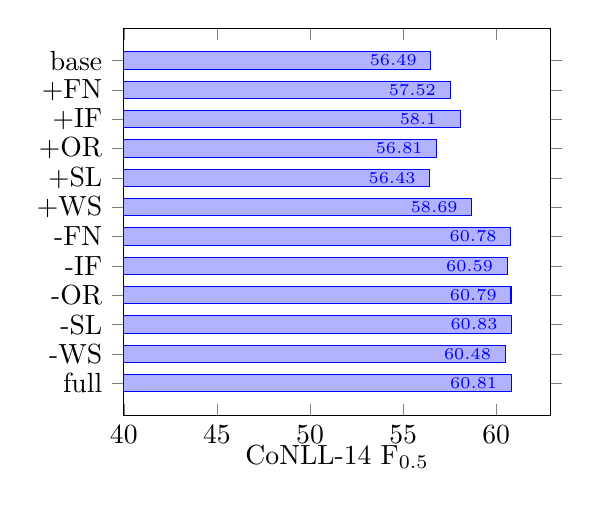
\begin{tikzpicture}
			\begin{axis}[
					xbar,
					xmin=40,
					%ymax=100,
					width=7cm,
					height=6.5cm,
					xlabel near ticks, xlabel shift={-6pt},
					ylabel near ticks, ylabel shift={-2pt},
					bar width=0.22cm,
					%enlargelimits=0.15,
					legend style={at={(0.5,-0.20)},
					anchor=north,legend columns=-1},
					xlabel={CoNLL-14 F${}_{0.5}$},
					ytick=data,
					symbolic y coords={full,-WS,-SL,-OR,-IF,-FN,+WS,+SL,+OR,+IF,+FN,base},
					nodes near coords,
					every node near coord/.append style={rotate=0, anchor=west, xshift=-0.9cm, font=\fontsize{6.5pt}{0.5pt}\selectfont},
				]
				\addplot coordinates {(56.49,base) (57.52,+FN) (58.10,+IF) (56.81,+OR) (56.43,+SL) (58.69,+WS) (60.78,-FN) (60.59,-IF) (60.79,-OR) (60.83,-SL) (60.48,-WS) (60.81,full)};
			\end{axis}
		\end{tikzpicture}
	\end{figure}
	\vspace{-1em}
	\begin{figure}[H]
		\centering
		\small
		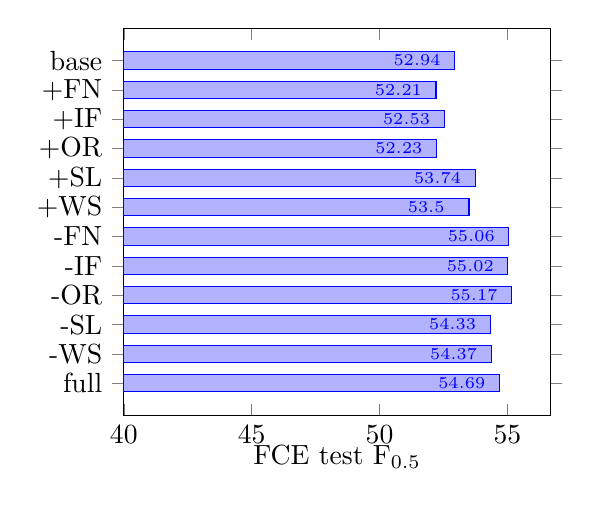
\begin{tikzpicture}
			\begin{axis}[
					xbar,
					xmin=40,
					%ymax=100,
					width=7cm,
					height=6.5cm,
					xlabel near ticks, xlabel shift={-6pt},
					ylabel near ticks, ylabel shift={-2pt},
					bar width=0.22cm,
					%enlargelimits=0.15,
					legend style={at={(0.5,-0.20)},
					anchor=north,legend columns=-1},
					xlabel={FCE test F${}_{0.5}$},
					ytick=data,
					symbolic y coords={full,-WS,-SL,-OR,-IF,-FN,+WS,+SL,+OR,+IF,+FN,base},
					nodes near coords,
					every node near coord/.append style={rotate=0, anchor=west, xshift=-0.9cm, font=\fontsize{6.5pt}{0.5pt}\selectfont},
				]
				\addplot coordinates {(52.94,base) (52.21,+FN) (52.53,+IF) (52.23,+OR) (53.74,+SL) (53.50,+WS) (55.06,-FN) (55.02,-IF) (55.17,-OR) (54.33,-SL) (54.37,-WS) (54.69,full)};
			\end{axis}
		\end{tikzpicture}
	\end{figure}
	\vspace{-1em}
	\begin{figure}[H]
		\centering
		\small
		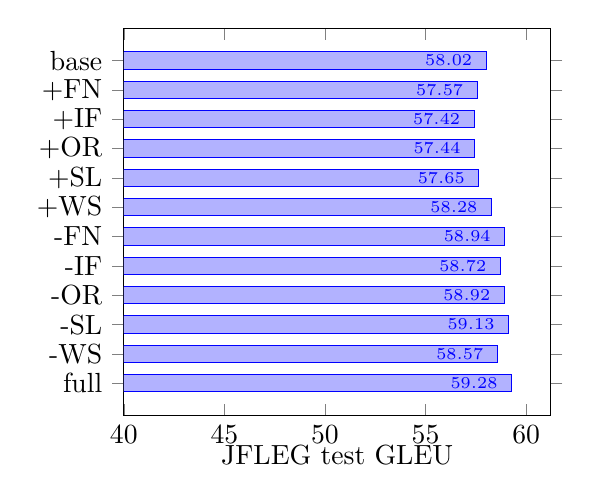
\begin{tikzpicture}
			\begin{axis}[
					xbar,
					xmin=40,
					%ymax=100,
					width=7cm,
					height=6.5cm,
					xlabel near ticks, xlabel shift={-6pt},
					ylabel near ticks, ylabel shift={-2pt},
					bar width=0.22cm,
					%enlargelimits=0.15,
					legend style={at={(0.5,-0.20)},
					anchor=north,legend columns=-1},
					xlabel={JFLEG test GLEU},
					ytick=data,
					symbolic y coords={full,-WS,-SL,-OR,-IF,-FN,+WS,+SL,+OR,+IF,+FN,base},
					nodes near coords,
					every node near coord/.append style={rotate=0, anchor=west, xshift=-0.9cm, font=\fontsize{6.5pt}{0.5pt}\selectfont},
				]
				\addplot coordinates {(58.02,base) (57.57,+FN) (57.42,+IF) (57.44,+OR) (57.65,+SL) (58.28,+WS) (58.94,-FN) (58.72,-IF) (58.92,-OR) (59.13,-SL) (58.57,-WS) (59.28,full)};
			\end{axis}
		\end{tikzpicture}
	\end{figure}
	\vspace{-1em}
	\begin{figure}[H]
		\centering
		\small
		8M x 10 epochs pre-training + fine-tuning (rescore) \\
		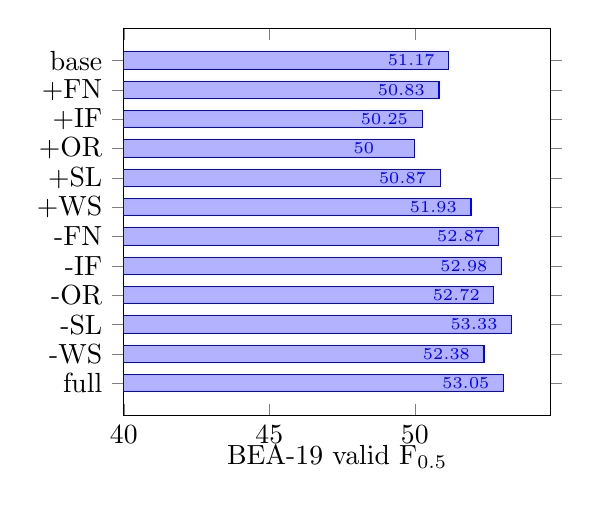
\begin{tikzpicture}
			\begin{axis}[
					xbar,
					xmin=40,
					%ymax=100,
					width=7cm,
					height=6.5cm,
					xlabel near ticks, xlabel shift={-6pt},
					ylabel near ticks, ylabel shift={-2pt},
					bar width=0.22cm,
					%enlargelimits=0.15,
					legend style={at={(0.5,-0.20)},
					anchor=north,legend columns=-1},
					xlabel={BEA-19 valid F${}_{0.5}$},
					ytick=data,
					symbolic y coords={full,-WS,-SL,-OR,-IF,-FN,+WS,+SL,+OR,+IF,+FN,base},
					nodes near coords,
					every node near coord/.append style={rotate=0, anchor=west, xshift=-0.9cm, font=\fontsize{6.5pt}{0.5pt}\selectfont},
				]
				\addplot coordinates {(51.17,base) (50.83,+FN) (50.25,+IF) (50.00,+OR) (50.87,+SL) (51.93,+WS) (52.87,-FN) (52.98,-IF) (52.72,-OR) (53.33,-SL) (52.38,-WS) (53.05,full)};
			\end{axis}
		\end{tikzpicture}
	\end{figure}
	\vspace{-1em}
	\begin{figure}[H]
		\centering
		\small
		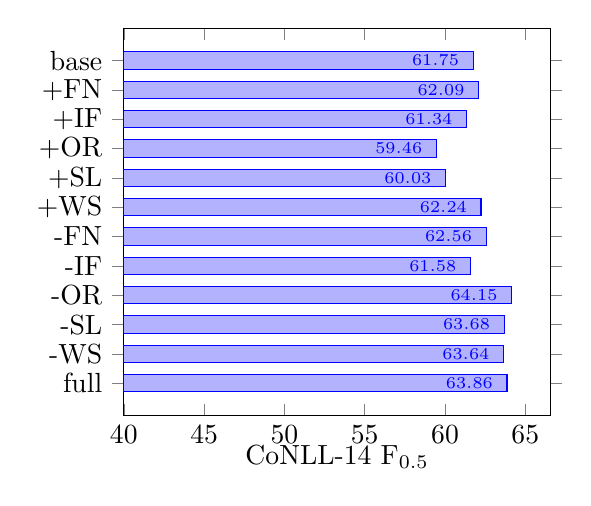
\begin{tikzpicture}
			\begin{axis}[
					xbar,
					xmin=40,
					%ymax=100,
					width=7cm,
					height=6.5cm,
					xlabel near ticks, xlabel shift={-6pt},
					ylabel near ticks, ylabel shift={-2pt},
					bar width=0.22cm,
					%enlargelimits=0.15,
					legend style={at={(0.5,-0.20)},
					anchor=north,legend columns=-1},
					xlabel={CoNLL-14 F${}_{0.5}$},
					ytick=data,
					symbolic y coords={full,-WS,-SL,-OR,-IF,-FN,+WS,+SL,+OR,+IF,+FN,base},
					nodes near coords,
					every node near coord/.append style={rotate=0, anchor=west, xshift=-0.9cm, font=\fontsize{6.5pt}{0.5pt}\selectfont},
				]
				\addplot coordinates {(61.75,base) (62.09,+FN) (61.34,+IF) (59.46,+OR) (60.03,+SL) (62.24,+WS) (62.56,-FN) (61.58,-IF) (64.15,-OR) (63.68,-SL) (63.64,-WS) (63.86,full)};
			\end{axis}
		\end{tikzpicture}
	\end{figure}
	\vspace{-1em}
	\begin{figure}[H]
		\centering
		\small
		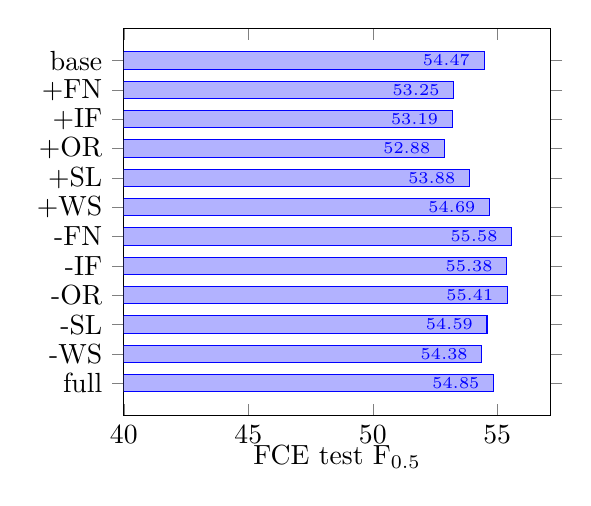
\begin{tikzpicture}
			\begin{axis}[
					xbar,
					xmin=40,
					%ymax=100,
					width=7cm,
					height=6.5cm,
					xlabel near ticks, xlabel shift={-6pt},
					ylabel near ticks, ylabel shift={-2pt},
					bar width=0.22cm,
					%enlargelimits=0.15,
					legend style={at={(0.5,-0.20)},
					anchor=north,legend columns=-1},
					xlabel={FCE test F${}_{0.5}$},
					ytick=data,
					symbolic y coords={full,-WS,-SL,-OR,-IF,-FN,+WS,+SL,+OR,+IF,+FN,base},
					nodes near coords,
					every node near coord/.append style={rotate=0, anchor=west, xshift=-0.9cm, font=\fontsize{6.5pt}{0.5pt}\selectfont},
				]
				\addplot coordinates {(54.47,base) (53.25,+FN) (53.19,+IF) (52.88,+OR) (53.88,+SL) (54.69,+WS) (55.58,-FN) (55.38,-IF) (55.41,-OR) (54.59,-SL) (54.38,-WS) (54.85,full)};
			\end{axis}
		\end{tikzpicture}
	\end{figure}
	\vspace{-1em}
	\begin{figure}[H]
		\centering
		\small
		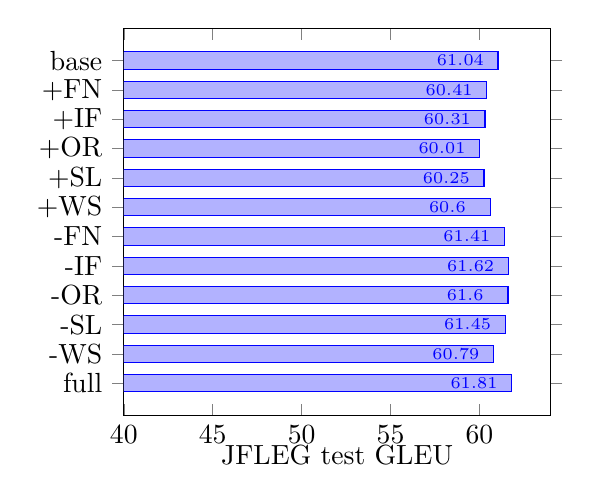
\begin{tikzpicture}
			\begin{axis}[
					xbar,
					xmin=40,
					%ymax=100,
					width=7cm,
					height=6.5cm,
					xlabel near ticks, xlabel shift={-6pt},
					ylabel near ticks, ylabel shift={-2pt},
					bar width=0.22cm,
					%enlargelimits=0.15,
					legend style={at={(0.5,-0.20)},
					anchor=north,legend columns=-1},
					xlabel={JFLEG test GLEU},
					ytick=data,
					symbolic y coords={full,-WS,-SL,-OR,-IF,-FN,+WS,+SL,+OR,+IF,+FN,base},
					nodes near coords,
					every node near coord/.append style={rotate=0, anchor=west, xshift=-0.9cm, font=\fontsize{6.5pt}{0.5pt}\selectfont},
				]
				\addplot coordinates {(61.04,base) (60.41,+FN) (60.31,+IF) (60.01,+OR) (60.25,+SL) (60.60,+WS) (61.41,-FN) (61.62,-IF) (61.60,-OR) (61.45,-SL) (60.79,-WS) (61.81,full)};
			\end{axis}
		\end{tikzpicture}
	\end{figure}
\end{multicols}

\newpage

\begin{figure}[H]
	\centering
	\footnotesize
	baseline \\
	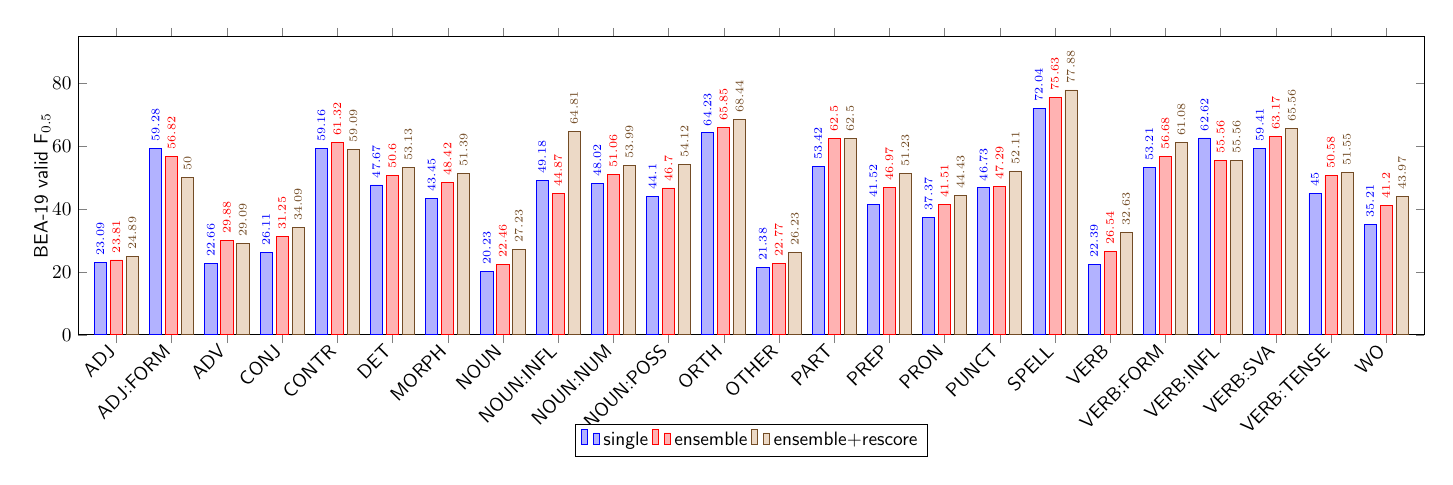
\begin{tikzpicture}[>=latex,font=\sffamily,scale=0.7,transform shape]
		\begin{axis}[
				ybar,
				ymin=0,
				ymax=95,
				width=26cm,
				height=7.0cm,
				xlabel near ticks, xlabel shift={-2pt},
				ylabel near ticks, ylabel shift={-6pt},
				enlarge x limits=0.03,
				bar width=0.22cm,
				legend style={at={(0.5,-0.30)}, anchor=north,legend columns=-1},
				ylabel={BEA-19 valid F${}_{0.5}$},
				symbolic x coords={ADJ,ADJ:FORM,ADV,CONJ,CONTR,DET,MORPH,NOUN,NOUN:INFL,NOUN:NUM,NOUN:POSS,ORTH,OTHER,PART,PREP,PRON,PUNCT,SPELL,VERB,VERB:FORM,VERB:INFL,VERB:SVA,VERB:TENSE,WO},
				xtick=data,
				x tick label style={rotate=45,anchor=east},
				nodes near coords,
				every node near coord/.append style={rotate=90, anchor=west, xshift=-0cm, font=\fontsize{6.5pt}{0.5pt}\selectfont},
			]
			\addplot coordinates {(ADJ,23.09) (ADJ:FORM,59.28) (ADV,22.66) (CONJ,26.11) (CONTR,59.16) (DET,47.67) (MORPH,43.45) (NOUN,20.23) (NOUN:INFL,49.18) (NOUN:NUM,48.02) (NOUN:POSS,44.10) (ORTH,64.23)
					(OTHER,21.38) (PART,53.42) (PREP,41.52) (PRON,37.37) (PUNCT,46.73) (SPELL,72.04) (VERB,22.39) (VERB:FORM,53.21) (VERB:INFL,62.62) (VERB:SVA,59.41) (VERB:TENSE,45.00) (WO,35.21)};
			\addplot coordinates {(ADJ,23.81) (ADJ:FORM,56.82) (ADV,29.88) (CONJ,31.25) (CONTR,61.32) (DET,50.60) (MORPH,48.42) (NOUN,22.46) (NOUN:INFL,44.87) (NOUN:NUM,51.06) (NOUN:POSS,46.70) (ORTH,65.85)
					(OTHER,22.77) (PART,62.50) (PREP,46.97) (PRON,41.51) (PUNCT,47.29) (SPELL,75.63) (VERB,26.54) (VERB:FORM,56.68) (VERB:INFL,55.56) (VERB:SVA,63.17) (VERB:TENSE,50.58) (WO,41.20)};
			\addplot coordinates {(ADJ,24.89) (ADJ:FORM,50.00) (ADV,29.09) (CONJ,34.09) (CONTR,59.09) (DET,53.13) (MORPH,51.39) (NOUN,27.23) (NOUN:INFL,64.81) (NOUN:NUM,53.99) (NOUN:POSS,54.12) (ORTH,68.44)
					(OTHER,26.23) (PART,62.50) (PREP,51.23) (PRON,44.43) (PUNCT,52.11) (SPELL,77.88) (VERB,32.63) (VERB:FORM,61.08) (VERB:INFL,55.56) (VERB:SVA,65.56) (VERB:TENSE,51.55) (WO,43.97)};
			\legend{single, ensemble, ensemble+rescore}
		\end{axis}
	\end{tikzpicture}
\end{figure}

\begin{figure}[H]
	\centering
	\footnotesize
	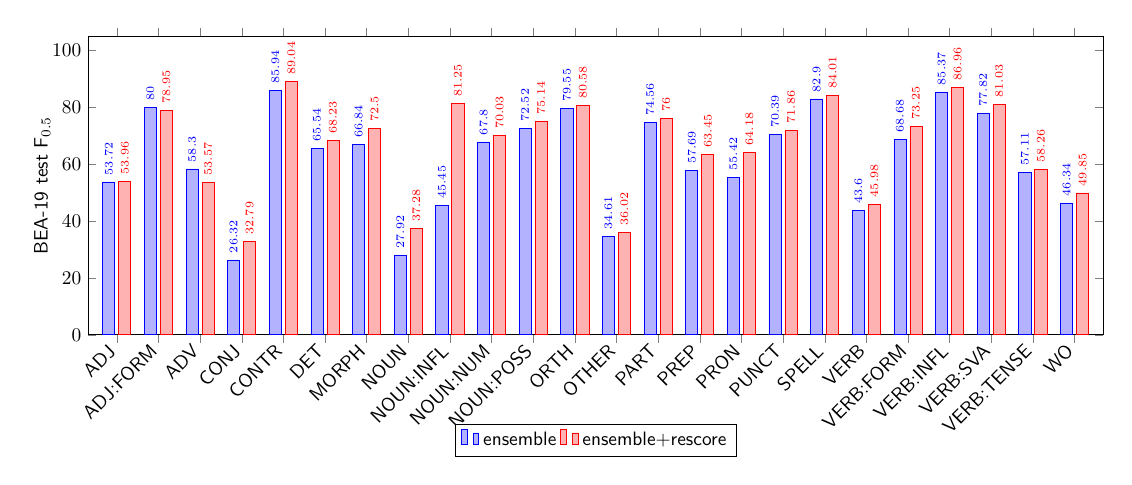
\begin{tikzpicture}[>=latex,font=\sffamily,scale=0.7,transform shape]
		\begin{axis}[
				ybar,
				ymin=0,
				ymax=105,
				width=20cm,
				height=7.0cm,
				xlabel near ticks, xlabel shift={-2pt},
				ylabel near ticks, ylabel shift={-6pt},
				enlarge x limits=0.03,
				bar width=0.22cm,
				legend style={at={(0.5,-0.30)}, anchor=north,legend columns=-1},
				ylabel={BEA-19 test F${}_{0.5}$},
				symbolic x coords={ADJ,ADJ:FORM,ADV,CONJ,CONTR,DET,MORPH,NOUN,NOUN:INFL,NOUN:NUM,NOUN:POSS,ORTH,OTHER,PART,PREP,PRON,PUNCT,SPELL,VERB,VERB:FORM,VERB:INFL,VERB:SVA,VERB:TENSE,WO},
				xtick=data,
				x tick label style={rotate=45,anchor=east},
				nodes near coords,
				every node near coord/.append style={rotate=90, anchor=west, xshift=-0cm, font=\fontsize{6.5pt}{0.5pt}\selectfont},
			]
			\addplot coordinates {(ADJ,53.72) (ADJ:FORM,80.00) (ADV,58.30) (CONJ,26.32) (CONTR,85.94) (DET,65.54) (MORPH,66.84) (NOUN,27.92) (NOUN:INFL,45.45) (NOUN:NUM,67.80) (NOUN:POSS,72.52) (ORTH,79.55)
					(OTHER,34.61) (PART,74.56) (PREP,57.69) (PRON,55.42) (PUNCT,70.39) (SPELL,82.90) (VERB,43.60) (VERB:FORM,68.68) (VERB:INFL,85.37) (VERB:SVA,77.82) (VERB:TENSE,57.11) (WO,46.34)};
			\addplot coordinates {(ADJ,53.96) (ADJ:FORM,78.95) (ADV,53.57) (CONJ,32.79) (CONTR,89.04) (DET,68.23) (MORPH,72.50) (NOUN,37.28) (NOUN:INFL,81.25) (NOUN:NUM,70.03) (NOUN:POSS,75.14) (ORTH,80.58)
					(OTHER,36.02) (PART,76.00) (PREP,63.45) (PRON,64.18) (PUNCT,71.86) (SPELL,84.01) (VERB,45.98) (VERB:FORM,73.25) (VERB:INFL,86.96) (VERB:SVA,81.03) (VERB:TENSE,58.26) (WO,49.85)};
			\legend{ensemble, ensemble+rescore}
		\end{axis}
	\end{tikzpicture}
\end{figure}

\begin{figure}[H]
	\centering
	\footnotesize
	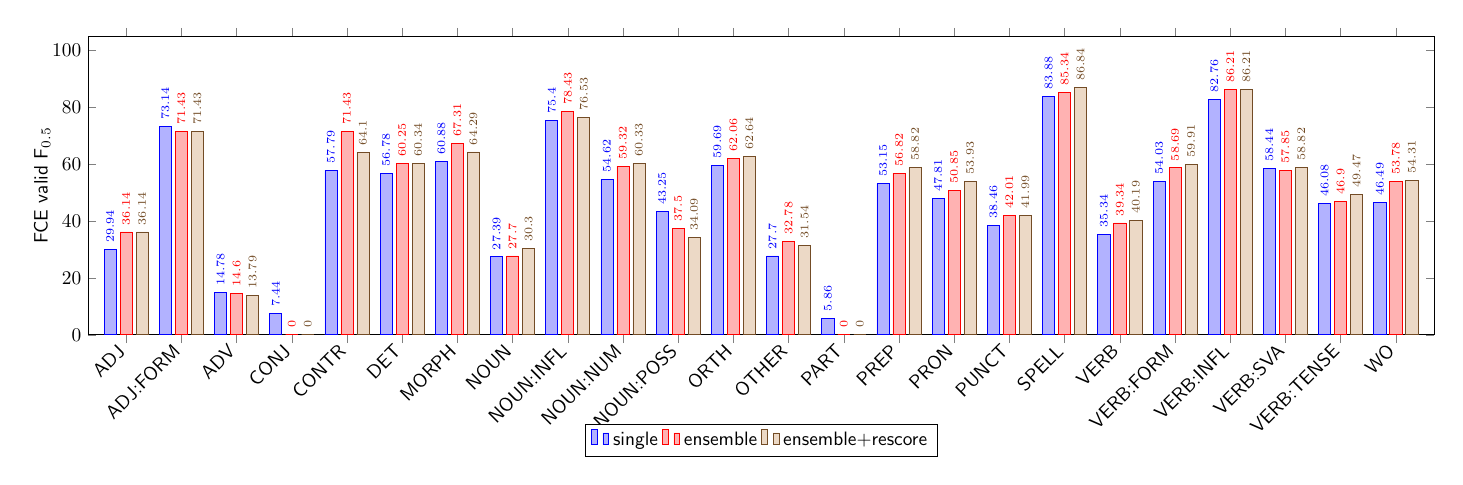
\begin{tikzpicture}[>=latex,font=\sffamily,scale=0.7,transform shape]
		\begin{axis}[
				ybar,
				ymin=0,
				ymax=105,
				width=26cm,
				height=7.0cm,
				xlabel near ticks, xlabel shift={-2pt},
				ylabel near ticks, ylabel shift={-6pt},
				enlarge x limits=0.03,
				bar width=0.22cm,
				legend style={at={(0.5,-0.30)}, anchor=north,legend columns=-1},
				ylabel={FCE valid F${}_{0.5}$},
				symbolic x coords={ADJ,ADJ:FORM,ADV,CONJ,CONTR,DET,MORPH,NOUN,NOUN:INFL,NOUN:NUM,NOUN:POSS,ORTH,OTHER,PART,PREP,PRON,PUNCT,SPELL,VERB,VERB:FORM,VERB:INFL,VERB:SVA,VERB:TENSE,WO},
				xtick=data,
				x tick label style={rotate=45,anchor=east},
				nodes near coords,
				every node near coord/.append style={rotate=90, anchor=west, xshift=-0cm, font=\fontsize{6.5pt}{0.5pt}\selectfont},
			]
			\addplot coordinates {(ADJ,29.94) (ADJ:FORM,73.14) (ADV,14.78) (CONJ,7.44) (CONTR,57.79) (DET,56.78) (MORPH,60.88) (NOUN,27.39) (NOUN:INFL,75.40) (NOUN:NUM,54.62) (NOUN:POSS,43.25) (ORTH,59.69)
					(OTHER,27.70) (PART,5.86) (PREP,53.15) (PRON,47.81) (PUNCT,38.46) (SPELL,83.88) (VERB,35.34) (VERB:FORM,54.03) (VERB:INFL,82.76) (VERB:SVA,58.44) (VERB:TENSE,46.08) (WO,46.49)};
			\addplot coordinates {(ADJ,36.14) (ADJ:FORM,71.43) (ADV,14.60) (CONJ,0.00) (CONTR,71.43) (DET,60.25) (MORPH,67.31) (NOUN,27.70) (NOUN:INFL,78.43) (NOUN:NUM,59.32) (NOUN:POSS,37.50) (ORTH,62.06)
					(OTHER,32.78) (PART,0.00) (PREP,56.82) (PRON,50.85) (PUNCT,42.01) (SPELL,85.34) (VERB,39.34) (VERB:FORM,58.69) (VERB:INFL,86.21) (VERB:SVA,57.85) (VERB:TENSE,46.90) (WO,53.78)};
			\addplot coordinates {(ADJ,36.14) (ADJ:FORM,71.43) (ADV,13.79) (CONJ,0.00) (CONTR,64.10) (DET,60.34) (MORPH,64.29) (NOUN,30.30) (NOUN:INFL,76.53) (NOUN:NUM,60.33) (NOUN:POSS,34.09) (ORTH,62.64)
					(OTHER,31.54) (PART,0.00) (PREP,58.82) (PRON,53.93) (PUNCT,41.99) (SPELL,86.84) (VERB,40.19) (VERB:FORM,59.91) (VERB:INFL,86.21) (VERB:SVA,58.82) (VERB:TENSE,49.47) (WO,54.31)};
			\legend{single, ensemble, ensemble+rescore}
		\end{axis}
	\end{tikzpicture}
\end{figure}

\begin{figure}[H]
	\centering
	\footnotesize
	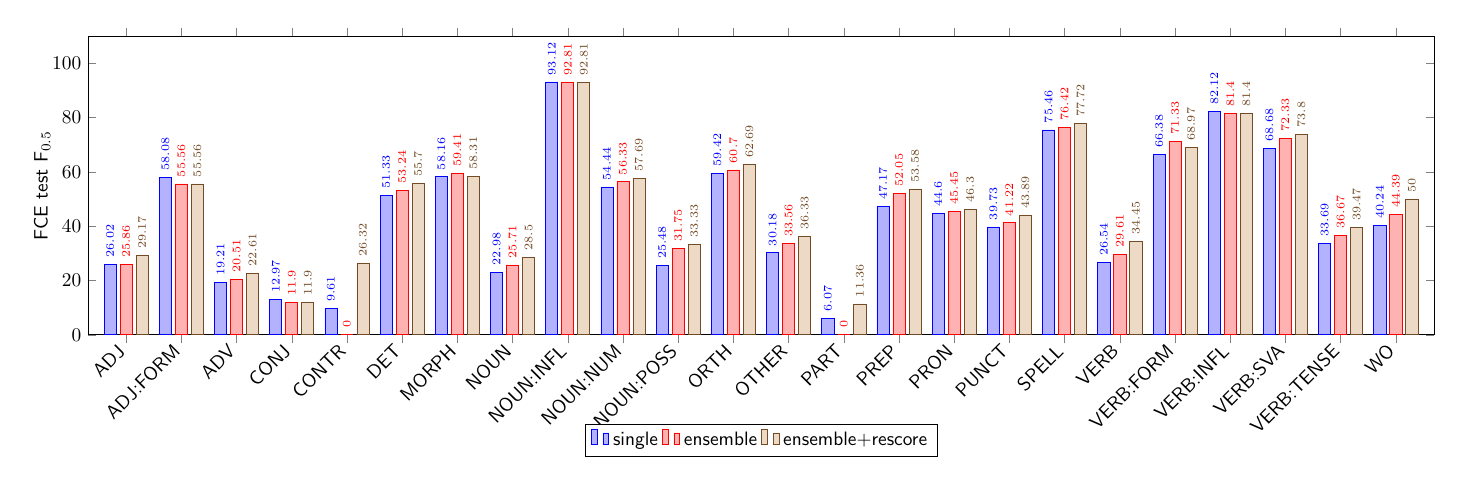
\begin{tikzpicture}[>=latex,font=\sffamily,scale=0.7,transform shape]
		\begin{axis}[
				ybar,
				ymin=0,
				ymax=110,
				width=26cm,
				height=7.0cm,
				xlabel near ticks, xlabel shift={-2pt},
				ylabel near ticks, ylabel shift={-6pt},
				enlarge x limits=0.03,
				bar width=0.22cm,
				legend style={at={(0.5,-0.30)}, anchor=north,legend columns=-1},
				ylabel={FCE test F${}_{0.5}$},
				symbolic x coords={ADJ,ADJ:FORM,ADV,CONJ,CONTR,DET,MORPH,NOUN,NOUN:INFL,NOUN:NUM,NOUN:POSS,ORTH,OTHER,PART,PREP,PRON,PUNCT,SPELL,VERB,VERB:FORM,VERB:INFL,VERB:SVA,VERB:TENSE,WO},
				xtick=data,
				x tick label style={rotate=45,anchor=east},
				nodes near coords,
				every node near coord/.append style={rotate=90, anchor=west, xshift=-0cm, font=\fontsize{6.5pt}{0.5pt}\selectfont},
			]
			\addplot coordinates {(ADJ,26.02) (ADJ:FORM,58.08) (ADV,19.21) (CONJ,12.97) (CONTR,9.61) (DET,51.33) (MORPH,58.16) (NOUN,22.98) (NOUN:INFL,93.12) (NOUN:NUM,54.44) (NOUN:POSS,25.48) (ORTH,59.42)
					(OTHER,30.18) (PART,6.07) (PREP,47.17) (PRON,44.60) (PUNCT,39.73) (SPELL,75.46) (VERB,26.54) (VERB:FORM,66.38) (VERB:INFL,82.12) (VERB:SVA,68.68) (VERB:TENSE,33.69) (WO,40.24)};
			\addplot coordinates {(ADJ,25.86) (ADJ:FORM,55.56) (ADV,20.51) (CONJ,11.90) (CONTR,0.00) (DET,53.24) (MORPH,59.41) (NOUN,25.71) (NOUN:INFL,92.81) (NOUN:NUM,56.33) (NOUN:POSS,31.75) (ORTH,60.70)
					(OTHER,33.56) (PART,0.00) (PREP,52.05) (PRON,45.45) (PUNCT,41.22) (SPELL,76.42) (VERB,29.61) (VERB:FORM,71.33) (VERB:INFL,81.40) (VERB:SVA,72.33) (VERB:TENSE,36.67) (WO,44.39)};
			\addplot coordinates {(ADJ,29.17) (ADJ:FORM,55.56) (ADV,22.61) (CONJ,11.90) (CONTR,26.32) (DET,55.70) (MORPH,58.31) (NOUN,28.50) (NOUN:INFL,92.81) (NOUN:NUM,57.69) (NOUN:POSS,33.33) (ORTH,62.69)
					(OTHER,36.33) (PART,11.36) (PREP,53.58) (PRON,46.30) (PUNCT,43.89) (SPELL,77.72) (VERB,34.45) (VERB:FORM,68.97) (VERB:INFL,81.40) (VERB:SVA,73.80) (VERB:TENSE,39.47) (WO,50.00)};
			\legend{single, ensemble, ensemble+rescore}
		\end{axis}
	\end{tikzpicture}
\end{figure}

\newpage

\begin{figure}[H]
	\centering
	\footnotesize
	pre-training \\
	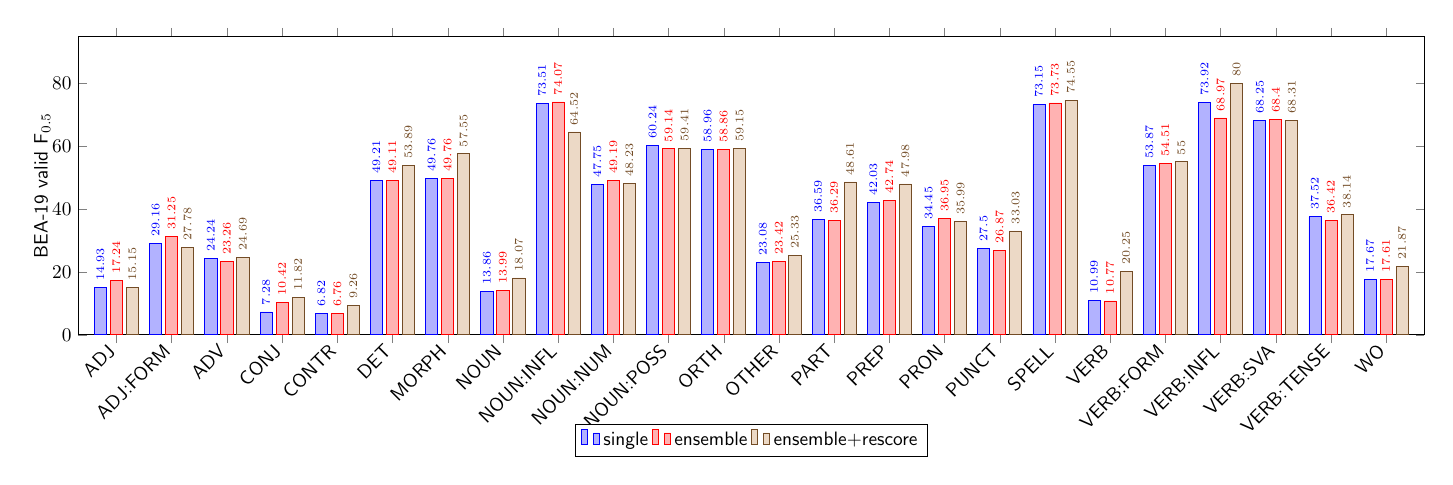
\begin{tikzpicture}[>=latex,font=\sffamily,scale=0.7,transform shape]
		\begin{axis}[
				ybar,
				ymin=0,
				ymax=95,
				width=26cm,
				height=7.0cm,
				xlabel near ticks, xlabel shift={-2pt},
				ylabel near ticks, ylabel shift={-6pt},
				enlarge x limits=0.03,
				bar width=0.22cm,
				legend style={at={(0.5,-0.30)}, anchor=north,legend columns=-1},
				ylabel={BEA-19 valid F${}_{0.5}$},
				symbolic x coords={ADJ,ADJ:FORM,ADV,CONJ,CONTR,DET,MORPH,NOUN,NOUN:INFL,NOUN:NUM,NOUN:POSS,ORTH,OTHER,PART,PREP,PRON,PUNCT,SPELL,VERB,VERB:FORM,VERB:INFL,VERB:SVA,VERB:TENSE,WO},
				xtick=data,
				x tick label style={rotate=45,anchor=east},
				nodes near coords,
				every node near coord/.append style={rotate=90, anchor=west, xshift=-0cm, font=\fontsize{6.5pt}{0.5pt}\selectfont},
			]
			\addplot coordinates {(ADJ,14.93) (ADJ:FORM,29.16) (ADV,24.24) (CONJ,7.28) (CONTR,6.82) (DET,49.21) (MORPH,49.76) (NOUN,13.86) (NOUN:INFL,73.51) (NOUN:NUM,47.75) (NOUN:POSS,60.24) (ORTH,58.96)
					(OTHER,23.08) (PART,36.59) (PREP,42.03) (PRON,34.45) (PUNCT,27.50) (SPELL,73.15) (VERB,10.99) (VERB:FORM,53.87) (VERB:INFL,73.92) (VERB:SVA,68.25) (VERB:TENSE,37.52) (WO,17.67)};
			\addplot coordinates {(ADJ,17.24) (ADJ:FORM,31.25) (ADV,23.26) (CONJ,10.42) (CONTR,6.76) (DET,49.11) (MORPH,49.76) (NOUN,13.99) (NOUN:INFL,74.07) (NOUN:NUM,49.19) (NOUN:POSS,59.14) (ORTH,58.86)
					(OTHER,23.42) (PART,36.29) (PREP,42.74) (PRON,36.95) (PUNCT,26.87) (SPELL,73.73) (VERB,10.77) (VERB:FORM,54.51) (VERB:INFL,68.97) (VERB:SVA,68.40) (VERB:TENSE,36.42) (WO,17.61)};
			\addplot coordinates {(ADJ,15.15) (ADJ:FORM,27.78) (ADV,24.69) (CONJ,11.82) (CONTR,9.26) (DET,53.89) (MORPH,57.55) (NOUN,18.07) (NOUN:INFL,64.52) (NOUN:NUM,48.23) (NOUN:POSS,59.41) (ORTH,59.15)
					(OTHER,25.33) (PART,48.61) (PREP,47.98) (PRON,35.99) (PUNCT,33.03) (SPELL,74.55) (VERB,20.25) (VERB:FORM,55.00) (VERB:INFL,80.00) (VERB:SVA,68.31) (VERB:TENSE,38.14) (WO,21.87)};
			\legend{single, ensemble, ensemble+rescore}
		\end{axis}
	\end{tikzpicture}
\end{figure}

\begin{figure}[H]
	\centering
	\footnotesize
	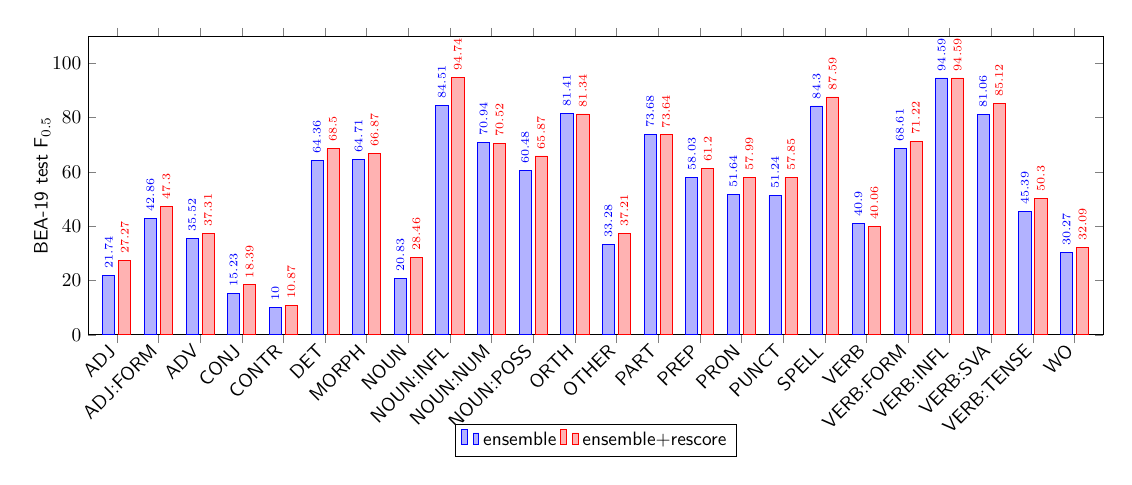
\begin{tikzpicture}[>=latex,font=\sffamily,scale=0.7,transform shape]
		\begin{axis}[
				ybar,
				ymin=0,
				ymax=110,
				width=20cm,
				height=7.0cm,
				xlabel near ticks, xlabel shift={-2pt},
				ylabel near ticks, ylabel shift={-6pt},
				enlarge x limits=0.03,
				bar width=0.22cm,
				legend style={at={(0.5,-0.30)}, anchor=north,legend columns=-1},
				ylabel={BEA-19 test F${}_{0.5}$},
				symbolic x coords={ADJ,ADJ:FORM,ADV,CONJ,CONTR,DET,MORPH,NOUN,NOUN:INFL,NOUN:NUM,NOUN:POSS,ORTH,OTHER,PART,PREP,PRON,PUNCT,SPELL,VERB,VERB:FORM,VERB:INFL,VERB:SVA,VERB:TENSE,WO},
				xtick=data,
				x tick label style={rotate=45,anchor=east},
				nodes near coords,
				every node near coord/.append style={rotate=90, anchor=west, xshift=-0cm, font=\fontsize{6.5pt}{0.5pt}\selectfont},
			]
			\addplot coordinates {(ADJ,21.74) (ADJ:FORM,42.86) (ADV,35.52) (CONJ,15.23) (CONTR,10.00) (DET,64.36) (MORPH,64.71) (NOUN,20.83) (NOUN:INFL,84.51) (NOUN:NUM,70.94) (NOUN:POSS,60.48) (ORTH,81.41)
					(OTHER,33.28) (PART,73.68) (PREP,58.03) (PRON,51.64) (PUNCT,51.24) (SPELL,84.30) (VERB,40.90) (VERB:FORM,68.61) (VERB:INFL,94.59) (VERB:SVA,81.06) (VERB:TENSE,45.39) (WO,30.27)};
			\addplot coordinates {(ADJ,27.27) (ADJ:FORM,47.30) (ADV,37.31) (CONJ,18.39) (CONTR,10.87) (DET,68.50) (MORPH,66.87) (NOUN,28.46) (NOUN:INFL,94.74) (NOUN:NUM,70.52) (NOUN:POSS,65.87) (ORTH,81.34)
					(OTHER,37.21) (PART,73.64) (PREP,61.20) (PRON,57.99) (PUNCT,57.85) (SPELL,87.59) (VERB,40.06) (VERB:FORM,71.22) (VERB:INFL,94.59) (VERB:SVA,85.12) (VERB:TENSE,50.30) (WO,32.09)};
			\legend{ensemble, ensemble+rescore}
		\end{axis}
	\end{tikzpicture}
\end{figure}

\begin{figure}[H]
	\centering
	\footnotesize
	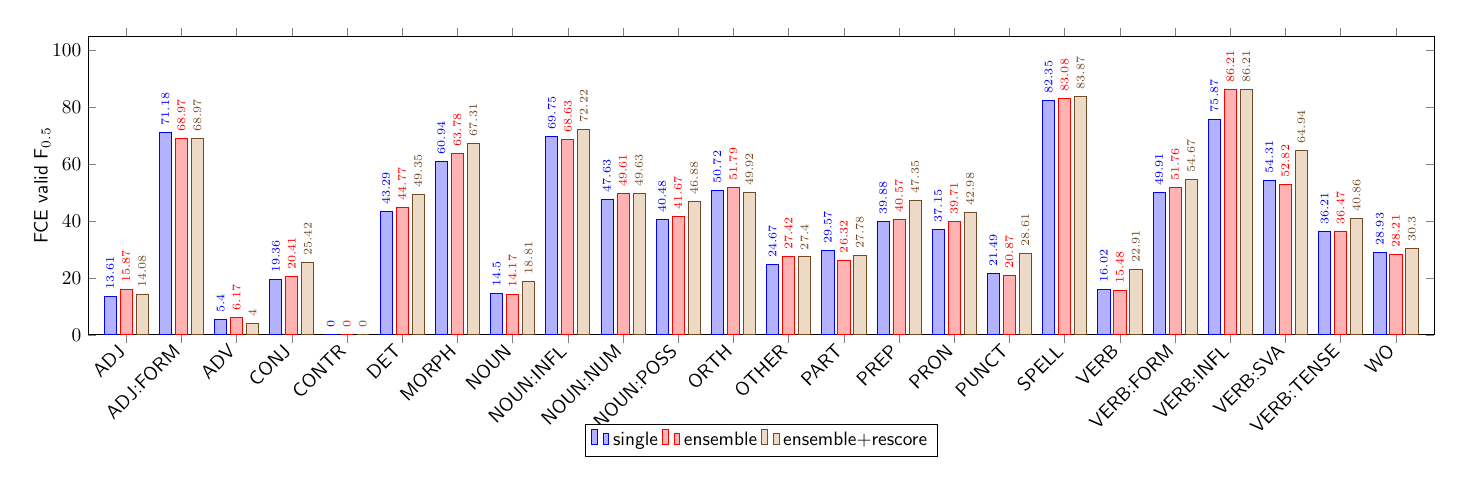
\begin{tikzpicture}[>=latex,font=\sffamily,scale=0.7,transform shape]
		\begin{axis}[
				ybar,
				ymin=0,
				ymax=105,
				width=26cm,
				height=7.0cm,
				xlabel near ticks, xlabel shift={-2pt},
				ylabel near ticks, ylabel shift={-6pt},
				enlarge x limits=0.03,
				bar width=0.22cm,
				legend style={at={(0.5,-0.30)}, anchor=north,legend columns=-1},
				ylabel={FCE valid F${}_{0.5}$},
				symbolic x coords={ADJ,ADJ:FORM,ADV,CONJ,CONTR,DET,MORPH,NOUN,NOUN:INFL,NOUN:NUM,NOUN:POSS,ORTH,OTHER,PART,PREP,PRON,PUNCT,SPELL,VERB,VERB:FORM,VERB:INFL,VERB:SVA,VERB:TENSE,WO},
				xtick=data,
				x tick label style={rotate=45,anchor=east},
				nodes near coords,
				every node near coord/.append style={rotate=90, anchor=west, xshift=-0cm, font=\fontsize{6.5pt}{0.5pt}\selectfont},
			]
			\addplot coordinates {(ADJ,13.61) (ADJ:FORM,71.18) (ADV,5.40) (CONJ,19.36) (CONTR,0.00) (DET,43.29) (MORPH,60.94) (NOUN,14.50) (NOUN:INFL,69.75) (NOUN:NUM,47.63) (NOUN:POSS,40.48) (ORTH,50.72)
					(OTHER,24.67) (PART,29.57) (PREP,39.88) (PRON,37.15) (PUNCT,21.49) (SPELL,82.35) (VERB,16.02) (VERB:FORM,49.91) (VERB:INFL,75.87) (VERB:SVA,54.31) (VERB:TENSE,36.21) (WO,28.93)};
			\addplot coordinates {(ADJ,15.87) (ADJ:FORM,68.97) (ADV,6.17) (CONJ,20.41) (CONTR,0.00) (DET,44.77) (MORPH,63.78) (NOUN,14.17) (NOUN:INFL,68.63) (NOUN:NUM,49.61) (NOUN:POSS,41.67) (ORTH,51.79)
					(OTHER,27.42) (PART,26.32) (PREP,40.57) (PRON,39.71) (PUNCT,20.87) (SPELL,83.08) (VERB,15.48) (VERB:FORM,51.76) (VERB:INFL,86.21) (VERB:SVA,52.82) (VERB:TENSE,36.47) (WO,28.21)};
			\addplot coordinates {(ADJ,14.08) (ADJ:FORM,68.97) (ADV,4.00) (CONJ,25.42) (CONTR,0.00) (DET,49.35) (MORPH,67.31) (NOUN,18.81) (NOUN:INFL,72.22) (NOUN:NUM,49.63) (NOUN:POSS,46.88) (ORTH,49.92)
					(OTHER,27.40) (PART,27.78) (PREP,47.35) (PRON,42.98) (PUNCT,28.61) (SPELL,83.87) (VERB,22.91) (VERB:FORM,54.67) (VERB:INFL,86.21) (VERB:SVA,64.94) (VERB:TENSE,40.86) (WO,30.30)};
			\legend{single, ensemble, ensemble+rescore}
		\end{axis}
	\end{tikzpicture}
\end{figure}

\begin{figure}[H]
	\centering
	\footnotesize
	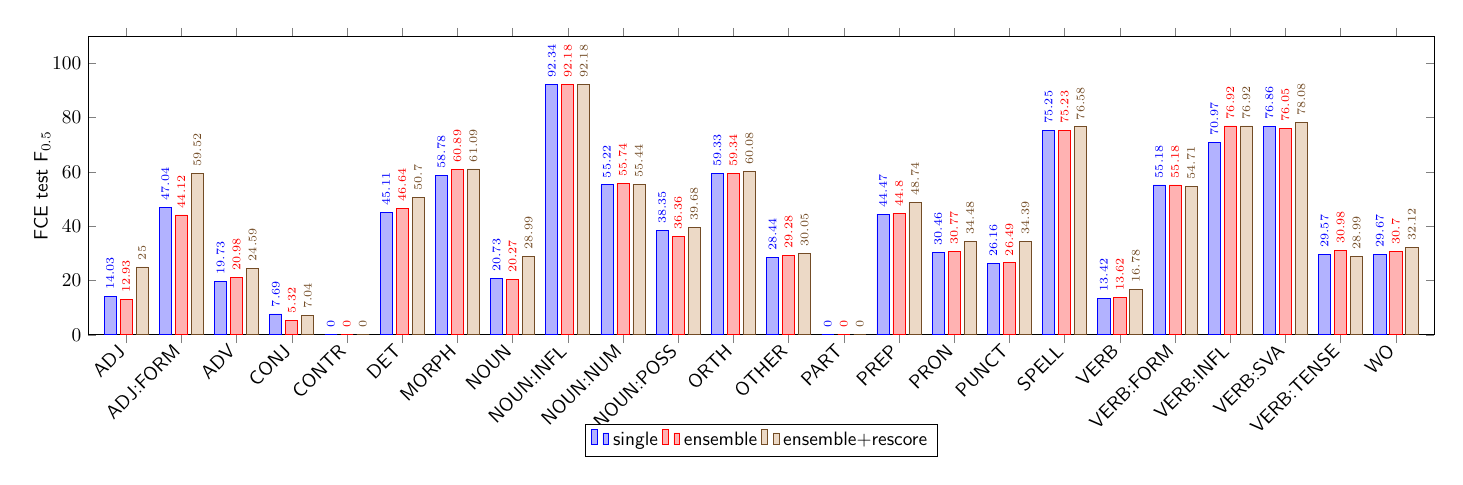
\begin{tikzpicture}[>=latex,font=\sffamily,scale=0.7,transform shape]
		\begin{axis}[
				ybar,
				ymin=0,
				ymax=110,
				width=26cm,
				height=7.0cm,
				xlabel near ticks, xlabel shift={-2pt},
				ylabel near ticks, ylabel shift={-6pt},
				enlarge x limits=0.03,
				bar width=0.22cm,
				legend style={at={(0.5,-0.30)}, anchor=north,legend columns=-1},
				ylabel={FCE test F${}_{0.5}$},
				symbolic x coords={ADJ,ADJ:FORM,ADV,CONJ,CONTR,DET,MORPH,NOUN,NOUN:INFL,NOUN:NUM,NOUN:POSS,ORTH,OTHER,PART,PREP,PRON,PUNCT,SPELL,VERB,VERB:FORM,VERB:INFL,VERB:SVA,VERB:TENSE,WO},
				xtick=data,
				x tick label style={rotate=45,anchor=east},
				nodes near coords,
				every node near coord/.append style={rotate=90, anchor=west, xshift=-0cm, font=\fontsize{6.5pt}{0.5pt}\selectfont},
			]
			\addplot coordinates {(ADJ,14.03) (ADJ:FORM,47.04) (ADV,19.73) (CONJ,7.69) (CONTR,0.00) (DET,45.11) (MORPH,58.78) (NOUN,20.73) (NOUN:INFL,92.34) (NOUN:NUM,55.22) (NOUN:POSS,38.35) (ORTH,59.33)
					(OTHER,28.44) (PART,0.00) (PREP,44.47) (PRON,30.46) (PUNCT,26.16) (SPELL,75.25) (VERB,13.42) (VERB:FORM,55.18) (VERB:INFL,70.97) (VERB:SVA,76.86) (VERB:TENSE,29.57) (WO,29.67)};
			\addplot coordinates {(ADJ,12.93) (ADJ:FORM,44.12) (ADV,20.98) (CONJ,5.32) (CONTR,0.00) (DET,46.64) (MORPH,60.89) (NOUN,20.27) (NOUN:INFL,92.18) (NOUN:NUM,55.74) (NOUN:POSS,36.36) (ORTH,59.34)
					(OTHER,29.28) (PART,0.00) (PREP,44.80) (PRON,30.77) (PUNCT,26.49) (SPELL,75.23) (VERB,13.62) (VERB:FORM,55.18) (VERB:INFL,76.92) (VERB:SVA,76.05) (VERB:TENSE,30.98) (WO,30.70)};
			\addplot coordinates {(ADJ,25.00) (ADJ:FORM,59.52) (ADV,24.59) (CONJ,7.04) (CONTR,0.00) (DET,50.70) (MORPH,61.09) (NOUN,28.99) (NOUN:INFL,92.18) (NOUN:NUM,55.44) (NOUN:POSS,39.68) (ORTH,60.08)
					(OTHER,30.05) (PART,0.00) (PREP,48.74) (PRON,34.48) (PUNCT,34.39) (SPELL,76.58) (VERB,16.78) (VERB:FORM,54.71) (VERB:INFL,76.92) (VERB:SVA,78.08) (VERB:TENSE,28.99) (WO,32.12)};
			\legend{single, ensemble, ensemble+rescore}
		\end{axis}
	\end{tikzpicture}
\end{figure}

\newpage

\begin{figure}[H]
	\centering
	\footnotesize
	pre-training + fine-tuning \\
	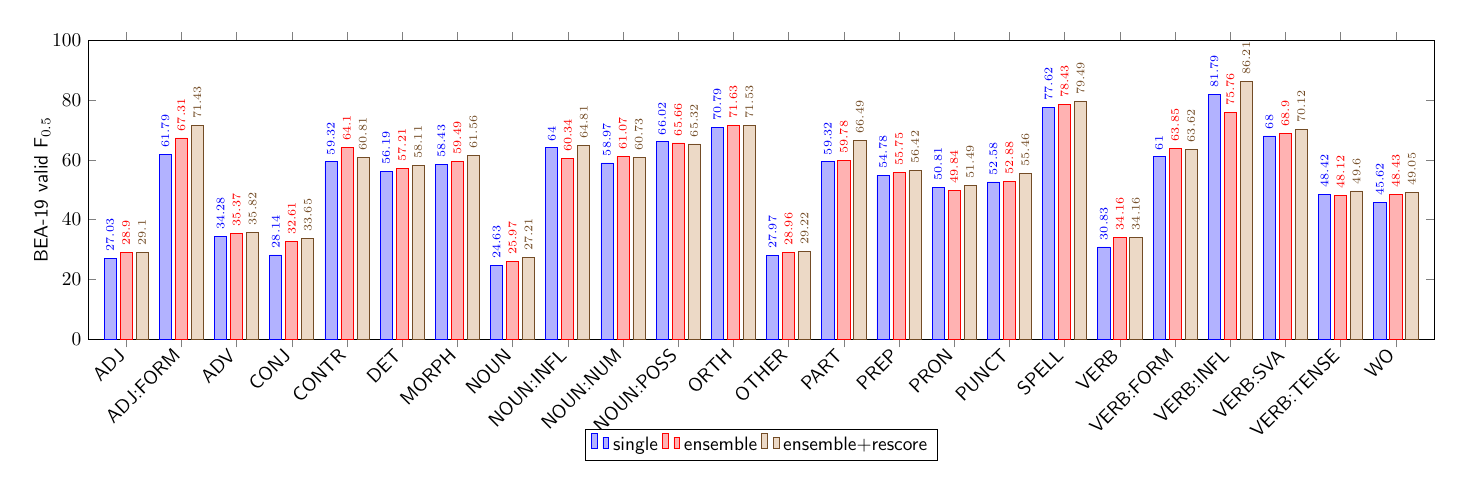
\begin{tikzpicture}[>=latex,font=\sffamily,scale=0.7,transform shape]
		\begin{axis}[
				ybar,
				ymin=0,
				ymax=100,
				width=26cm,
				height=7.0cm,
				xlabel near ticks, xlabel shift={-2pt},
				ylabel near ticks, ylabel shift={-6pt},
				enlarge x limits=0.03,
				bar width=0.22cm,
				legend style={at={(0.5,-0.30)}, anchor=north,legend columns=-1},
				ylabel={BEA-19 valid F${}_{0.5}$},
				symbolic x coords={ADJ,ADJ:FORM,ADV,CONJ,CONTR,DET,MORPH,NOUN,NOUN:INFL,NOUN:NUM,NOUN:POSS,ORTH,OTHER,PART,PREP,PRON,PUNCT,SPELL,VERB,VERB:FORM,VERB:INFL,VERB:SVA,VERB:TENSE,WO},
				xtick=data,
				x tick label style={rotate=45,anchor=east},
				nodes near coords,
				every node near coord/.append style={rotate=90, anchor=west, xshift=-0cm, font=\fontsize{6.5pt}{0.5pt}\selectfont},
			]
			\addplot coordinates {(ADJ,27.03) (ADJ:FORM,61.79) (ADV,34.28) (CONJ,28.14) (CONTR,59.32) (DET,56.19) (MORPH,58.43) (NOUN,24.63) (NOUN:INFL,64.00) (NOUN:NUM,58.97) (NOUN:POSS,66.02) (ORTH,70.79)
					(OTHER,27.97) (PART,59.32) (PREP,54.78) (PRON,50.81) (PUNCT,52.58) (SPELL,77.62) (VERB,30.83) (VERB:FORM,61.00) (VERB:INFL,81.79) (VERB:SVA,68.00) (VERB:TENSE,48.42) (WO,45.62)};
			\addplot coordinates {(ADJ,28.90) (ADJ:FORM,67.31) (ADV,35.37) (CONJ,32.61) (CONTR,64.10) (DET,57.21) (MORPH,59.49) (NOUN,25.97) (NOUN:INFL,60.34) (NOUN:NUM,61.07) (NOUN:POSS,65.66) (ORTH,71.63)
					(OTHER,28.96) (PART,59.78) (PREP,55.75) (PRON,49.84) (PUNCT,52.88) (SPELL,78.43) (VERB,34.16) (VERB:FORM,63.85) (VERB:INFL,75.76) (VERB:SVA,68.90) (VERB:TENSE,48.12) (WO,48.43)};
			\addplot coordinates {(ADJ,29.10) (ADJ:FORM,71.43) (ADV,35.82) (CONJ,33.65) (CONTR,60.81) (DET,58.11) (MORPH,61.56) (NOUN,27.21) (NOUN:INFL,64.81) (NOUN:NUM,60.73) (NOUN:POSS,65.32) (ORTH,71.53)
					(OTHER,29.22) (PART,66.49) (PREP,56.42) (PRON,51.49) (PUNCT,55.46) (SPELL,79.49) (VERB,34.16) (VERB:FORM,63.62) (VERB:INFL,86.21) (VERB:SVA,70.12) (VERB:TENSE,49.60) (WO,49.05)};
			\legend{single, ensemble, ensemble+rescore}
		\end{axis}
	\end{tikzpicture}
\end{figure}

\begin{figure}[H]
	\centering
	\footnotesize
	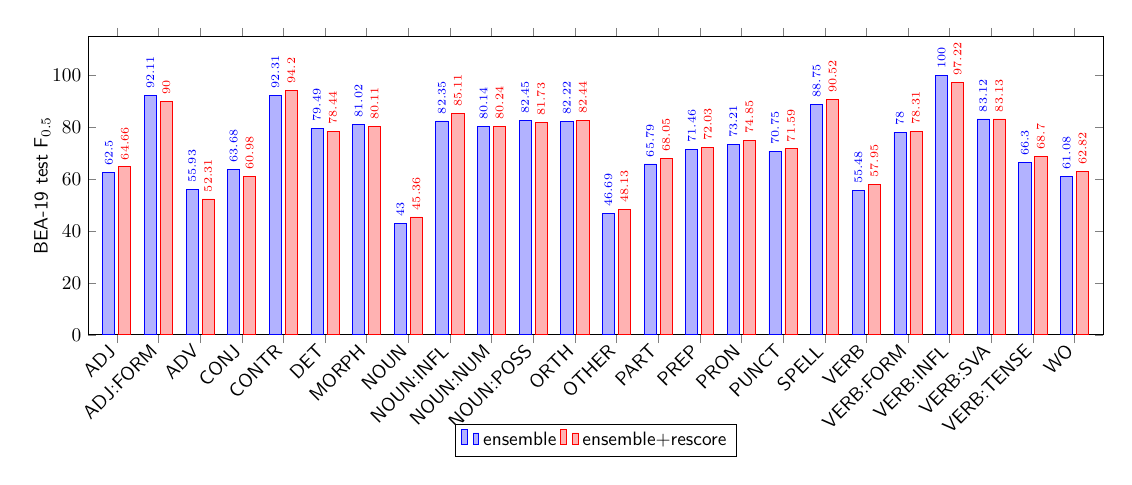
\begin{tikzpicture}[>=latex,font=\sffamily,scale=0.7,transform shape]
		\begin{axis}[
				ybar,
				ymin=0,
				ymax=115,
				width=20cm,
				height=7.0cm,
				xlabel near ticks, xlabel shift={-2pt},
				ylabel near ticks, ylabel shift={-6pt},
				enlarge x limits=0.03,
				bar width=0.22cm,
				legend style={at={(0.5,-0.30)}, anchor=north,legend columns=-1},
				ylabel={BEA-19 test F${}_{0.5}$},
				symbolic x coords={ADJ,ADJ:FORM,ADV,CONJ,CONTR,DET,MORPH,NOUN,NOUN:INFL,NOUN:NUM,NOUN:POSS,ORTH,OTHER,PART,PREP,PRON,PUNCT,SPELL,VERB,VERB:FORM,VERB:INFL,VERB:SVA,VERB:TENSE,WO},
				xtick=data,
				x tick label style={rotate=45,anchor=east},
				nodes near coords,
				every node near coord/.append style={rotate=90, anchor=west, xshift=-0cm, font=\fontsize{6.5pt}{0.5pt}\selectfont},
			]
			\addplot coordinates {(ADJ,62.50) (ADJ:FORM,92.11) (ADV,55.93) (CONJ,63.68) (CONTR,92.31) (DET,79.49) (MORPH,81.02) (NOUN,43.00) (NOUN:INFL,82.35) (NOUN:NUM,80.14) (NOUN:POSS,82.45) (ORTH,82.22)
					(OTHER,46.69) (PART,65.79) (PREP,71.46) (PRON,73.21) (PUNCT,70.75) (SPELL,88.75) (VERB,55.48) (VERB:FORM,78.00) (VERB:INFL,100.00) (VERB:SVA,83.12) (VERB:TENSE,66.30) (WO,61.08)};
			\addplot coordinates {(ADJ,64.66) (ADJ:FORM,90.00) (ADV,52.31) (CONJ,60.98) (CONTR,94.20) (DET,78.44) (MORPH,80.11) (NOUN,45.36) (NOUN:INFL,85.11) (NOUN:NUM,80.24) (NOUN:POSS,81.73) (ORTH,82.44)
					(OTHER,48.13) (PART,68.05) (PREP,72.03) (PRON,74.85) (PUNCT,71.59) (SPELL,90.52) (VERB,57.95) (VERB:FORM,78.31) (VERB:INFL,97.22) (VERB:SVA,83.13) (VERB:TENSE,68.70) (WO,62.82)};
			\legend{ensemble, ensemble+rescore}
		\end{axis}
	\end{tikzpicture}
\end{figure}

\begin{figure}[H]
	\centering
	\footnotesize
	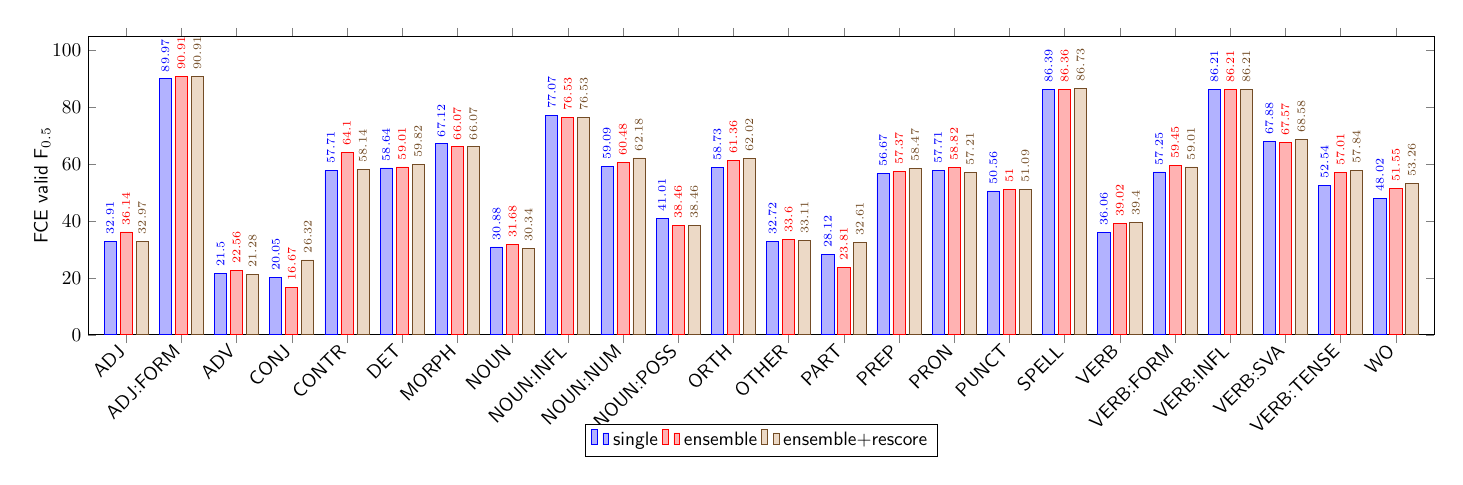
\begin{tikzpicture}[>=latex,font=\sffamily,scale=0.7,transform shape]
		\begin{axis}[
				ybar,
				ymin=0,
				ymax=105,
				width=26cm,
				height=7.0cm,
				xlabel near ticks, xlabel shift={-2pt},
				ylabel near ticks, ylabel shift={-6pt},
				enlarge x limits=0.03,
				bar width=0.22cm,
				legend style={at={(0.5,-0.30)}, anchor=north,legend columns=-1},
				ylabel={FCE valid F${}_{0.5}$},
				symbolic x coords={ADJ,ADJ:FORM,ADV,CONJ,CONTR,DET,MORPH,NOUN,NOUN:INFL,NOUN:NUM,NOUN:POSS,ORTH,OTHER,PART,PREP,PRON,PUNCT,SPELL,VERB,VERB:FORM,VERB:INFL,VERB:SVA,VERB:TENSE,WO},
				xtick=data,
				x tick label style={rotate=45,anchor=east},
				nodes near coords,
				every node near coord/.append style={rotate=90, anchor=west, xshift=-0cm, font=\fontsize{6.5pt}{0.5pt}\selectfont},
			]
			\addplot coordinates {(ADJ,32.91) (ADJ:FORM,89.97) (ADV,21.50) (CONJ,20.05) (CONTR,57.71) (DET,58.64) (MORPH,67.12) (NOUN,30.88) (NOUN:INFL,77.07) (NOUN:NUM,59.09) (NOUN:POSS,41.01) (ORTH,58.73)
					(OTHER,32.72) (PART,28.12) (PREP,56.67) (PRON,57.71) (PUNCT,50.56) (SPELL,86.39) (VERB,36.06) (VERB:FORM,57.25) (VERB:INFL,86.21) (VERB:SVA,67.88) (VERB:TENSE,52.54) (WO,48.02)};
			\addplot coordinates {(ADJ,36.14) (ADJ:FORM,90.91) (ADV,22.56) (CONJ,16.67) (CONTR,64.10) (DET,59.01) (MORPH,66.07) (NOUN,31.68) (NOUN:INFL,76.53) (NOUN:NUM,60.48) (NOUN:POSS,38.46) (ORTH,61.36)
					(OTHER,33.60) (PART,23.81) (PREP,57.37) (PRON,58.82) (PUNCT,51.00) (SPELL,86.36) (VERB,39.02) (VERB:FORM,59.45) (VERB:INFL,86.21) (VERB:SVA,67.57) (VERB:TENSE,57.01) (WO,51.55)};
			\addplot coordinates {(ADJ,32.97) (ADJ:FORM,90.91) (ADV,21.28) (CONJ,26.32) (CONTR,58.14) (DET,59.82) (MORPH,66.07) (NOUN,30.34) (NOUN:INFL,76.53) (NOUN:NUM,62.18) (NOUN:POSS,38.46) (ORTH,62.02)
					(OTHER,33.11) (PART,32.61) (PREP,58.47) (PRON,57.21) (PUNCT,51.09) (SPELL,86.73) (VERB,39.40) (VERB:FORM,59.01) (VERB:INFL,86.21) (VERB:SVA,68.58) (VERB:TENSE,57.84) (WO,53.26)};
			\legend{single, ensemble, ensemble+rescore}
		\end{axis}
	\end{tikzpicture}
\end{figure}

\begin{figure}[H]
	\centering
	\footnotesize
	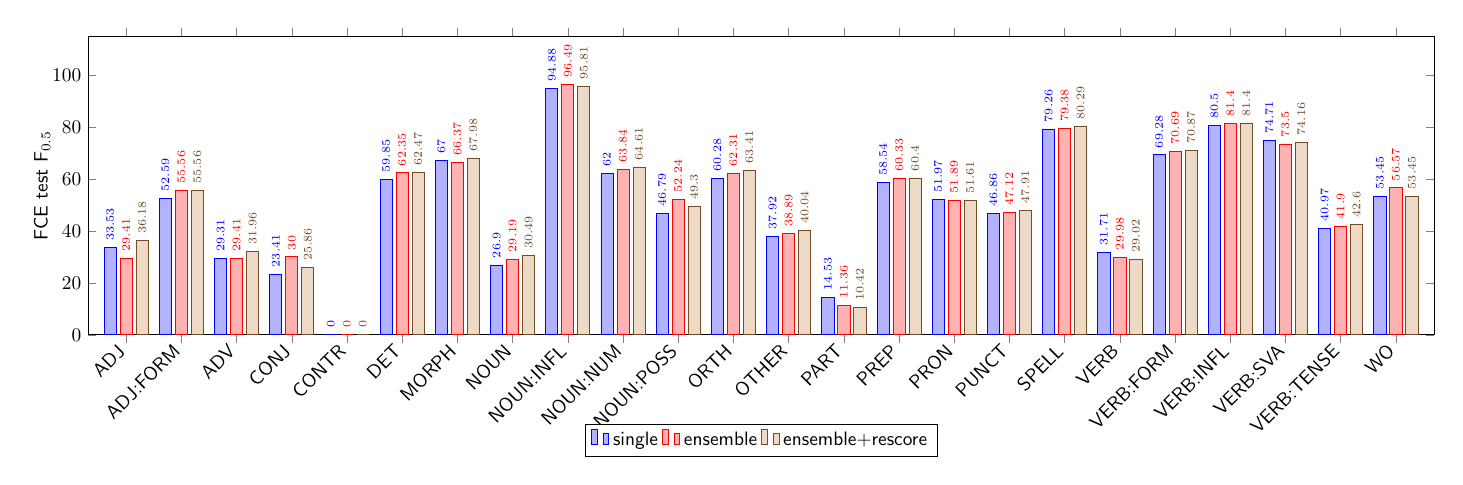
\begin{tikzpicture}[>=latex,font=\sffamily,scale=0.7,transform shape]
		\begin{axis}[
				ybar,
				ymin=0,
				ymax=115,
				width=26cm,
				height=7.0cm,
				xlabel near ticks, xlabel shift={-2pt},
				ylabel near ticks, ylabel shift={-6pt},
				enlarge x limits=0.03,
				bar width=0.22cm,
				legend style={at={(0.5,-0.30)}, anchor=north,legend columns=-1},
				ylabel={FCE test F${}_{0.5}$},
				symbolic x coords={ADJ,ADJ:FORM,ADV,CONJ,CONTR,DET,MORPH,NOUN,NOUN:INFL,NOUN:NUM,NOUN:POSS,ORTH,OTHER,PART,PREP,PRON,PUNCT,SPELL,VERB,VERB:FORM,VERB:INFL,VERB:SVA,VERB:TENSE,WO},
				xtick=data,
				x tick label style={rotate=45,anchor=east},
				nodes near coords,
				every node near coord/.append style={rotate=90, anchor=west, xshift=-0cm, font=\fontsize{6.5pt}{0.5pt}\selectfont},
			]
			\addplot coordinates {(ADJ,33.53) (ADJ:FORM,52.59) (ADV,29.31) (CONJ,23.41) (CONTR,0.00) (DET,59.85) (MORPH,67.00) (NOUN,26.90) (NOUN:INFL,94.88) (NOUN:NUM,62.00) (NOUN:POSS,46.79) (ORTH,60.28)
					(OTHER,37.92) (PART,14.53) (PREP,58.54) (PRON,51.97) (PUNCT,46.86) (SPELL,79.26) (VERB,31.71) (VERB:FORM,69.28) (VERB:INFL,80.50) (VERB:SVA,74.71) (VERB:TENSE,40.97) (WO,53.45)};
			\addplot coordinates {(ADJ,29.41) (ADJ:FORM,55.56) (ADV,29.41) (CONJ,30.00) (CONTR,0.00) (DET,62.35) (MORPH,66.37) (NOUN,29.19) (NOUN:INFL,96.49) (NOUN:NUM,63.84) (NOUN:POSS,52.24) (ORTH,62.31)
					(OTHER,38.89) (PART,11.36) (PREP,60.33) (PRON,51.89) (PUNCT,47.12) (SPELL,79.38) (VERB,29.98) (VERB:FORM,70.69) (VERB:INFL,81.40) (VERB:SVA,73.50) (VERB:TENSE,41.90) (WO,56.57)};
			\addplot coordinates {(ADJ,36.18) (ADJ:FORM,55.56) (ADV,31.96) (CONJ,25.86) (CONTR,0.00) (DET,62.47) (MORPH,67.98) (NOUN,30.49) (NOUN:INFL,95.81) (NOUN:NUM,64.61) (NOUN:POSS,49.30) (ORTH,63.41)
					(OTHER,40.04) (PART,10.42) (PREP,60.40) (PRON,51.61) (PUNCT,47.91) (SPELL,80.29) (VERB,29.02) (VERB:FORM,70.87) (VERB:INFL,81.40) (VERB:SVA,74.16) (VERB:TENSE,42.60) (WO,53.45)};
			\legend{single, ensemble, ensemble+rescore}
		\end{axis}
	\end{tikzpicture}
\end{figure}

\newpage

\begin{figure}[H]
	\centering
	\footnotesize
	pre-training + fine-tuning + domain adaptation \\
	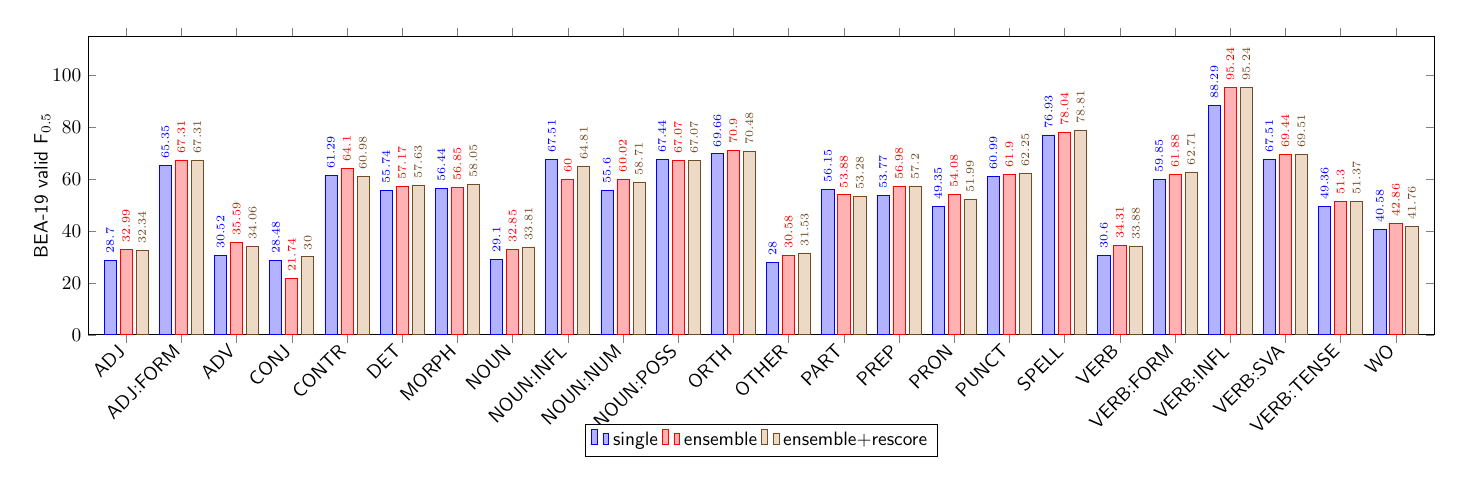
\begin{tikzpicture}[>=latex,font=\sffamily,scale=0.7,transform shape]
		\begin{axis}[
				ybar,
				ymin=0,
				ymax=115,
				width=26cm,
				height=7.0cm,
				xlabel near ticks, xlabel shift={-2pt},
				ylabel near ticks, ylabel shift={-6pt},
				enlarge x limits=0.03,
				bar width=0.22cm,
				legend style={at={(0.5,-0.30)}, anchor=north,legend columns=-1},
				ylabel={BEA-19 valid F${}_{0.5}$},
				symbolic x coords={ADJ,ADJ:FORM,ADV,CONJ,CONTR,DET,MORPH,NOUN,NOUN:INFL,NOUN:NUM,NOUN:POSS,ORTH,OTHER,PART,PREP,PRON,PUNCT,SPELL,VERB,VERB:FORM,VERB:INFL,VERB:SVA,VERB:TENSE,WO},
				xtick=data,
				x tick label style={rotate=45,anchor=east},
				nodes near coords,
				every node near coord/.append style={rotate=90, anchor=west, xshift=-0cm, font=\fontsize{6.5pt}{0.5pt}\selectfont},
			]
			\addplot coordinates {(ADJ,28.70) (ADJ:FORM,65.35) (ADV,30.52) (CONJ,28.48) (CONTR,61.29) (DET,55.74) (MORPH,56.44) (NOUN,29.10) (NOUN:INFL,67.51) (NOUN:NUM,55.60) (NOUN:POSS,67.44) (ORTH,69.66)
					(OTHER,28.00) (PART,56.15) (PREP,53.77) (PRON,49.35) (PUNCT,60.99) (SPELL,76.93) (VERB,30.60) (VERB:FORM,59.85) (VERB:INFL,88.29) (VERB:SVA,67.51) (VERB:TENSE,49.36) (WO,40.58)};
			\addplot coordinates {(ADJ,32.99) (ADJ:FORM,67.31) (ADV,35.59) (CONJ,21.74) (CONTR,64.10) (DET,57.17) (MORPH,56.85) (NOUN,32.85) (NOUN:INFL,60.00) (NOUN:NUM,60.02) (NOUN:POSS,67.07) (ORTH,70.90)
					(OTHER,30.58) (PART,53.88) (PREP,56.98) (PRON,54.08) (PUNCT,61.90) (SPELL,78.04) (VERB,34.31) (VERB:FORM,61.88) (VERB:INFL,95.24) (VERB:SVA,69.44) (VERB:TENSE,51.30) (WO,42.86)};
			\addplot coordinates {(ADJ,32.34) (ADJ:FORM,67.31) (ADV,34.06) (CONJ,30.00) (CONTR,60.98) (DET,57.63) (MORPH,58.05) (NOUN,33.81) (NOUN:INFL,64.81) (NOUN:NUM,58.71) (NOUN:POSS,67.07) (ORTH,70.48)
					(OTHER,31.53) (PART,53.28) (PREP,57.20) (PRON,51.99) (PUNCT,62.25) (SPELL,78.81) (VERB,33.88) (VERB:FORM,62.71) (VERB:INFL,95.24) (VERB:SVA,69.51) (VERB:TENSE,51.37) (WO,41.76)};
			\legend{single, ensemble, ensemble+rescore}
		\end{axis}
	\end{tikzpicture}
\end{figure}

\begin{figure}[H]
	\centering
	\footnotesize
	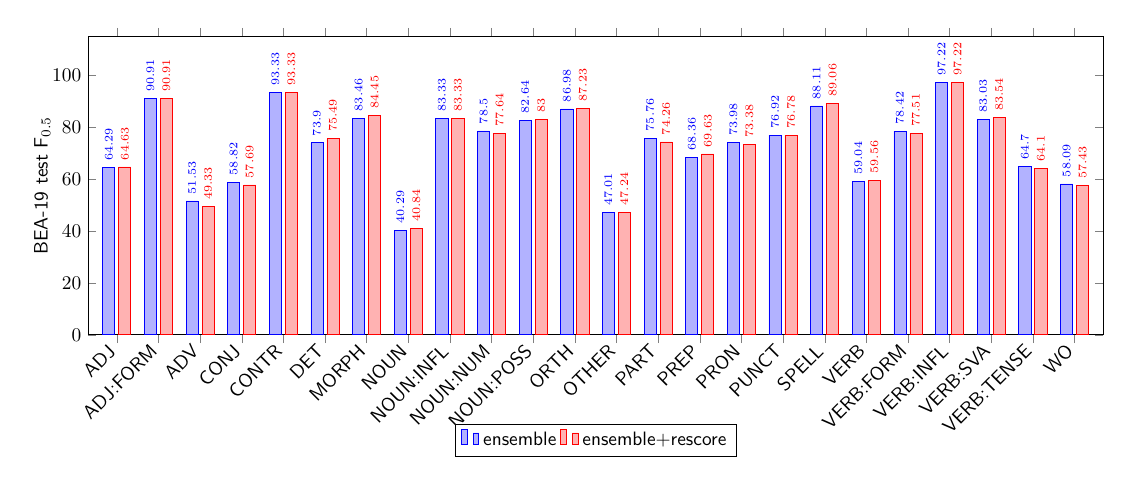
\begin{tikzpicture}[>=latex,font=\sffamily,scale=0.7,transform shape]
		\begin{axis}[
				ybar,
				ymin=0,
				ymax=115,
				width=20cm,
				height=7.0cm,
				xlabel near ticks, xlabel shift={-2pt},
				ylabel near ticks, ylabel shift={-6pt},
				enlarge x limits=0.03,
				bar width=0.22cm,
				legend style={at={(0.5,-0.30)}, anchor=north,legend columns=-1},
				ylabel={BEA-19 test F${}_{0.5}$},
				symbolic x coords={ADJ,ADJ:FORM,ADV,CONJ,CONTR,DET,MORPH,NOUN,NOUN:INFL,NOUN:NUM,NOUN:POSS,ORTH,OTHER,PART,PREP,PRON,PUNCT,SPELL,VERB,VERB:FORM,VERB:INFL,VERB:SVA,VERB:TENSE,WO},
				xtick=data,
				x tick label style={rotate=45,anchor=east},
				nodes near coords,
				every node near coord/.append style={rotate=90, anchor=west, xshift=-0cm, font=\fontsize{6.5pt}{0.5pt}\selectfont},
			]
			\addplot coordinates {(ADJ,64.29) (ADJ:FORM,90.91) (ADV,51.53) (CONJ,58.82) (CONTR,93.33) (DET,73.90) (MORPH,83.46) (NOUN,40.29) (NOUN:INFL,83.33) (NOUN:NUM,78.50) (NOUN:POSS,82.64) (ORTH,86.98)
					(OTHER,47.01) (PART,75.76) (PREP,68.36) (PRON,73.98) (PUNCT,76.92) (SPELL,88.11) (VERB,59.04) (VERB:FORM,78.42) (VERB:INFL,97.22) (VERB:SVA,83.03) (VERB:TENSE,64.70) (WO,58.09)};
			\addplot coordinates {(ADJ,64.63) (ADJ:FORM,90.91) (ADV,49.33) (CONJ,57.69) (CONTR,93.33) (DET,75.49) (MORPH,84.45) (NOUN,40.84) (NOUN:INFL,83.33) (NOUN:NUM,77.64) (NOUN:POSS,83.00) (ORTH,87.23)
					(OTHER,47.24) (PART,74.26) (PREP,69.63) (PRON,73.38) (PUNCT,76.78) (SPELL,89.06) (VERB,59.56) (VERB:FORM,77.51) (VERB:INFL,97.22) (VERB:SVA,83.54) (VERB:TENSE,64.10) (WO,57.43)};
			\legend{ensemble, ensemble+rescore}
		\end{axis}
	\end{tikzpicture}
\end{figure}

\begin{figure}[H]
	\centering
	\footnotesize
	\begin{tikzpicture}[>=latex,font=\sffamily,scale=0.7,transform shape]
		\begin{axis}[
				ybar,
				ymin=0,
				ymax=110,
				width=26cm,
				height=7.0cm,
				xlabel near ticks, xlabel shift={-2pt},
				ylabel near ticks, ylabel shift={-6pt},
				enlarge x limits=0.03,
				bar width=0.22cm,
				legend style={at={(0.5,-0.30)}, anchor=north,legend columns=-1},
				ylabel={FCE valid F${}_{0.5}$},
				symbolic x coords={ADJ,ADJ:FORM,ADV,CONJ,CONTR,DET,MORPH,NOUN,NOUN:INFL,NOUN:NUM,NOUN:POSS,ORTH,OTHER,PART,PREP,PRON,PUNCT,SPELL,VERB,VERB:FORM,VERB:INFL,VERB:SVA,VERB:TENSE,WO},
				xtick=data,
				x tick label style={rotate=45,anchor=east},
				nodes near coords,
				every node near coord/.append style={rotate=90, anchor=west, xshift=-0cm, font=\fontsize{6.5pt}{0.5pt}\selectfont},
			]
			\addplot coordinates {(ADJ,44.24) (ADJ:FORM,89.97) (ADV,19.82) (CONJ,20.14) (CONTR,60.52) (DET,60.14) (MORPH,64.42) (NOUN,35.94) (NOUN:INFL,78.95) (NOUN:NUM,60.60) (NOUN:POSS,44.17) (ORTH,63.32)
					(OTHER,32.84) (PART,27.23) (PREP,55.75) (PRON,54.23) (PUNCT,53.04) (SPELL,86.66) (VERB,36.82) (VERB:FORM,57.74) (VERB:INFL,91.73) (VERB:SVA,67.95) (VERB:TENSE,49.90) (WO,50.63)};
			\addplot coordinates {(ADJ,50.51) (ADJ:FORM,90.91) (ADV,22.56) (CONJ,14.71) (CONTR,64.10) (DET,61.54) (MORPH,67.43) (NOUN,36.18) (NOUN:INFL,78.43) (NOUN:NUM,61.31) (NOUN:POSS,44.64) (ORTH,66.13)
					(OTHER,34.03) (PART,24.19) (PREP,58.25) (PRON,58.14) (PUNCT,53.37) (SPELL,87.56) (VERB,38.14) (VERB:FORM,57.24) (VERB:INFL,86.21) (VERB:SVA,72.07) (VERB:TENSE,53.49) (WO,52.12)};
			\addplot coordinates {(ADJ,49.55) (ADJ:FORM,90.91) (ADV,21.28) (CONJ,14.71) (CONTR,58.14) (DET,61.43) (MORPH,63.27) (NOUN,37.08) (NOUN:INFL,78.43) (NOUN:NUM,63.03) (NOUN:POSS,46.88) (ORTH,68.34)
					(OTHER,33.49) (PART,24.19) (PREP,58.21) (PRON,59.79) (PUNCT,54.38) (SPELL,88.04) (VERB,38.21) (VERB:FORM,59.96) (VERB:INFL,86.21) (VERB:SVA,72.07) (VERB:TENSE,53.19) (WO,52.87)};
			\legend{single, ensemble, ensemble+rescore}
		\end{axis}
	\end{tikzpicture}
\end{figure}

\begin{figure}[H]
	\centering
	\footnotesize
	\begin{tikzpicture}[>=latex,font=\sffamily,scale=0.7,transform shape]
		\begin{axis}[
				ybar,
				ymin=0,
				ymax=115,
				width=26cm,
				height=7.0cm,
				xlabel near ticks, xlabel shift={-2pt},
				ylabel near ticks, ylabel shift={-6pt},
				enlarge x limits=0.03,
				bar width=0.22cm,
				legend style={at={(0.5,-0.30)}, anchor=north,legend columns=-1},
				ylabel={FCE test F${}_{0.5}$},
				symbolic x coords={ADJ,ADJ:FORM,ADV,CONJ,CONTR,DET,MORPH,NOUN,NOUN:INFL,NOUN:NUM,NOUN:POSS,ORTH,OTHER,PART,PREP,PRON,PUNCT,SPELL,VERB,VERB:FORM,VERB:INFL,VERB:SVA,VERB:TENSE,WO},
				xtick=data,
				x tick label style={rotate=45,anchor=east},
				nodes near coords,
				every node near coord/.append style={rotate=90, anchor=west, xshift=-0cm, font=\fontsize{6.5pt}{0.5pt}\selectfont},
			]
			\addplot coordinates {(ADJ,33.41) (ADJ:FORM,51.39) (ADV,31.12) (CONJ,19.04) (CONTR,14.35) (DET,61.34) (MORPH,66.01) (NOUN,31.34) (NOUN:INFL,95.99) (NOUN:NUM,61.39) (NOUN:POSS,44.25) (ORTH,67.74)
					(OTHER,37.99) (PART,12.72) (PREP,57.82) (PRON,51.73) (PUNCT,50.34) (SPELL,80.98) (VERB,31.36) (VERB:FORM,68.48) (VERB:INFL,84.86) (VERB:SVA,74.28) (VERB:TENSE,39.46) (WO,56.14)};
			\addplot coordinates {(ADJ,35.26) (ADJ:FORM,38.46) (ADV,26.74) (CONJ,27.78) (CONTR,0.00) (DET,62.58) (MORPH,64.10) (NOUN,32.26) (NOUN:INFL,96.49) (NOUN:NUM,63.54) (NOUN:POSS,48.54) (ORTH,67.49)
					(OTHER,41.23) (PART,8.93) (PREP,59.96) (PRON,52.52) (PUNCT,51.70) (SPELL,81.95) (VERB,35.21) (VERB:FORM,69.88) (VERB:INFL,90.91) (VERB:SVA,74.59) (VERB:TENSE,42.17) (WO,58.94)};
			\addplot coordinates {(ADJ,36.59) (ADJ:FORM,38.46) (ADV,30.77) (CONJ,27.78) (CONTR,33.33) (DET,63.63) (MORPH,66.20) (NOUN,32.75) (NOUN:INFL,97.14) (NOUN:NUM,63.21) (NOUN:POSS,47.83) (ORTH,67.72)
					(OTHER,39.84) (PART,10.42) (PREP,59.56) (PRON,53.42) (PUNCT,50.77) (SPELL,82.39) (VERB,31.67) (VERB:FORM,70.22) (VERB:INFL,90.91) (VERB:SVA,75.72) (VERB:TENSE,42.14) (WO,60.08)};
			\legend{single, ensemble, ensemble+rescore}
		\end{axis}
	\end{tikzpicture}
\end{figure}

\newpage

\begin{figure}[H]
	\centering
	\footnotesize
	single \\
	\begin{tikzpicture}[>=latex,font=\sffamily,scale=0.7,transform shape]
		\begin{axis}[
				ybar,
				ymin=0,
				ymax=115,
				width=26cm,
				height=7.0cm,
				xlabel near ticks, xlabel shift={-2pt},
				ylabel near ticks, ylabel shift={-6pt},
				enlarge x limits=0.03,
				bar width=0.22cm,
				legend style={at={(0.5,-0.30)}, anchor=north,legend columns=-1},
				ylabel={BEA-19 valid F${}_{0.5}$},
				symbolic x coords={ADJ,ADJ:FORM,ADV,CONJ,CONTR,DET,MORPH,NOUN,NOUN:INFL,NOUN:NUM,NOUN:POSS,ORTH,OTHER,PART,PREP,PRON,PUNCT,SPELL,VERB,VERB:FORM,VERB:INFL,VERB:SVA,VERB:TENSE,WO},
				xtick=data,
				x tick label style={rotate=45,anchor=east},
				nodes near coords,
				every node near coord/.append style={rotate=90, anchor=west, xshift=-0cm, font=\fontsize{6.5pt}{0.5pt}\selectfont},
			]
			\addplot coordinates {(ADJ,23.09) (ADJ:FORM,59.28) (ADV,22.66) (CONJ,26.11) (CONTR,59.16) (DET,47.67) (MORPH,43.45) (NOUN,20.23) (NOUN:INFL,49.18) (NOUN:NUM,48.02) (NOUN:POSS,44.10) (ORTH,64.23)
					(OTHER,21.38) (PART,53.42) (PREP,41.52) (PRON,37.37) (PUNCT,46.73) (SPELL,72.04) (VERB,22.39) (VERB:FORM,53.21) (VERB:INFL,62.62) (VERB:SVA,59.41) (VERB:TENSE,45.00) (WO,35.21)};
			\addplot coordinates {(ADJ,27.03) (ADJ:FORM,61.79) (ADV,34.28) (CONJ,28.14) (CONTR,59.32) (DET,56.19) (MORPH,58.43) (NOUN,24.63) (NOUN:INFL,64.00) (NOUN:NUM,58.97) (NOUN:POSS,66.02) (ORTH,70.79)
					(OTHER,27.97) (PART,59.32) (PREP,54.78) (PRON,50.81) (PUNCT,52.58) (SPELL,77.62) (VERB,30.83) (VERB:FORM,61.00) (VERB:INFL,81.79) (VERB:SVA,68.00) (VERB:TENSE,48.42) (WO,45.62)};
			\addplot coordinates {(ADJ,28.70) (ADJ:FORM,65.35) (ADV,30.52) (CONJ,28.48) (CONTR,61.29) (DET,55.74) (MORPH,56.44) (NOUN,29.10) (NOUN:INFL,67.51) (NOUN:NUM,55.60) (NOUN:POSS,67.44) (ORTH,69.66)
					(OTHER,28.00) (PART,56.15) (PREP,53.77) (PRON,49.35) (PUNCT,60.99) (SPELL,76.93) (VERB,30.60) (VERB:FORM,59.85) (VERB:INFL,88.29) (VERB:SVA,67.51) (VERB:TENSE,49.36) (WO,40.58)};
			\legend{baseline, pre-training + fine-tuning, pre-training + fine-tuning + domain adaptation}
		\end{axis}
	\end{tikzpicture}
\end{figure}

\begin{figure}[H]
	\centering
	\footnotesize
	\begin{tikzpicture}[>=latex,font=\sffamily,scale=0.7,transform shape]
		\begin{axis}[
				ybar,
				ymin=0,
				ymax=110,
				width=26cm,
				height=7.0cm,
				xlabel near ticks, xlabel shift={-2pt},
				ylabel near ticks, ylabel shift={-6pt},
				enlarge x limits=0.03,
				bar width=0.22cm,
				legend style={at={(0.5,-0.30)}, anchor=north,legend columns=-1},
				ylabel={FCE valid F${}_{0.5}$},
				symbolic x coords={ADJ,ADJ:FORM,ADV,CONJ,CONTR,DET,MORPH,NOUN,NOUN:INFL,NOUN:NUM,NOUN:POSS,ORTH,OTHER,PART,PREP,PRON,PUNCT,SPELL,VERB,VERB:FORM,VERB:INFL,VERB:SVA,VERB:TENSE,WO},
				xtick=data,
				x tick label style={rotate=45,anchor=east},
				nodes near coords,
				every node near coord/.append style={rotate=90, anchor=west, xshift=-0cm, font=\fontsize{6.5pt}{0.5pt}\selectfont},
			]
			\addplot coordinates {(ADJ,29.94) (ADJ:FORM,73.14) (ADV,14.78) (CONJ,7.44) (CONTR,57.79) (DET,56.78) (MORPH,60.88) (NOUN,27.39) (NOUN:INFL,75.40) (NOUN:NUM,54.62) (NOUN:POSS,43.25) (ORTH,59.69)
					(OTHER,27.70) (PART,5.86) (PREP,53.15) (PRON,47.81) (PUNCT,38.46) (SPELL,83.88) (VERB,35.34) (VERB:FORM,54.03) (VERB:INFL,82.76) (VERB:SVA,58.44) (VERB:TENSE,46.08) (WO,46.49)};
			\addplot coordinates {(ADJ,32.91) (ADJ:FORM,89.97) (ADV,21.50) (CONJ,20.05) (CONTR,57.71) (DET,58.64) (MORPH,67.12) (NOUN,30.88) (NOUN:INFL,77.07) (NOUN:NUM,59.09) (NOUN:POSS,41.01) (ORTH,58.73)
					(OTHER,32.72) (PART,28.12) (PREP,56.67) (PRON,57.71) (PUNCT,50.56) (SPELL,86.39) (VERB,36.06) (VERB:FORM,57.25) (VERB:INFL,86.21) (VERB:SVA,67.88) (VERB:TENSE,52.54) (WO,48.02)};
			\addplot coordinates {(ADJ,44.24) (ADJ:FORM,89.97) (ADV,19.82) (CONJ,20.14) (CONTR,60.52) (DET,60.14) (MORPH,64.42) (NOUN,35.94) (NOUN:INFL,78.95) (NOUN:NUM,60.60) (NOUN:POSS,44.17) (ORTH,63.32)
					(OTHER,32.84) (PART,27.23) (PREP,55.75) (PRON,54.23) (PUNCT,53.04) (SPELL,86.66) (VERB,36.82) (VERB:FORM,57.74) (VERB:INFL,91.73) (VERB:SVA,67.95) (VERB:TENSE,49.90) (WO,50.63)};
			\legend{baseline, pre-training + fine-tuning, pre-training + fine-tuning + domain adaptation}
		\end{axis}
	\end{tikzpicture}
\end{figure}

\begin{figure}[H]
	\centering
	\footnotesize
	\begin{tikzpicture}[>=latex,font=\sffamily,scale=0.7,transform shape]
		\begin{axis}[
				ybar,
				ymin=0,
				ymax=115,
				width=26cm,
				height=7.0cm,
				xlabel near ticks, xlabel shift={-2pt},
				ylabel near ticks, ylabel shift={-6pt},
				enlarge x limits=0.03,
				bar width=0.22cm,
				legend style={at={(0.5,-0.30)}, anchor=north,legend columns=-1},
				ylabel={FCE test F${}_{0.5}$},
				symbolic x coords={ADJ,ADJ:FORM,ADV,CONJ,CONTR,DET,MORPH,NOUN,NOUN:INFL,NOUN:NUM,NOUN:POSS,ORTH,OTHER,PART,PREP,PRON,PUNCT,SPELL,VERB,VERB:FORM,VERB:INFL,VERB:SVA,VERB:TENSE,WO},
				xtick=data,
				x tick label style={rotate=45,anchor=east},
				nodes near coords,
				every node near coord/.append style={rotate=90, anchor=west, xshift=-0cm, font=\fontsize{6.5pt}{0.5pt}\selectfont},
			]
			\addplot coordinates {(ADJ,26.02) (ADJ:FORM,58.08) (ADV,19.21) (CONJ,12.97) (CONTR,9.61) (DET,51.33) (MORPH,58.16) (NOUN,22.98) (NOUN:INFL,93.12) (NOUN:NUM,54.44) (NOUN:POSS,25.48) (ORTH,59.42)
					(OTHER,30.18) (PART,6.07) (PREP,47.17) (PRON,44.60) (PUNCT,39.73) (SPELL,75.46) (VERB,26.54) (VERB:FORM,66.38) (VERB:INFL,82.12) (VERB:SVA,68.68) (VERB:TENSE,33.69) (WO,40.24)};
			\addplot coordinates {(ADJ,33.53) (ADJ:FORM,52.59) (ADV,29.31) (CONJ,23.41) (CONTR,0.00) (DET,59.85) (MORPH,67.00) (NOUN,26.90) (NOUN:INFL,94.88) (NOUN:NUM,62.00) (NOUN:POSS,46.79) (ORTH,60.28)
					(OTHER,37.92) (PART,14.53) (PREP,58.54) (PRON,51.97) (PUNCT,46.86) (SPELL,79.26) (VERB,31.71) (VERB:FORM,69.28) (VERB:INFL,80.50) (VERB:SVA,74.71) (VERB:TENSE,40.97) (WO,53.45)};
			\addplot coordinates {(ADJ,33.41) (ADJ:FORM,51.39) (ADV,31.12) (CONJ,19.04) (CONTR,14.35) (DET,61.34) (MORPH,66.01) (NOUN,31.34) (NOUN:INFL,95.99) (NOUN:NUM,61.39) (NOUN:POSS,44.25) (ORTH,67.74)
					(OTHER,37.99) (PART,12.72) (PREP,57.82) (PRON,51.73) (PUNCT,50.34) (SPELL,80.98) (VERB,31.36) (VERB:FORM,68.48) (VERB:INFL,84.86) (VERB:SVA,74.28) (VERB:TENSE,39.46) (WO,56.14)};
			\legend{baseline, pre-training + fine-tuning, pre-training + fine-tuning + domain adaptation}
		\end{axis}
	\end{tikzpicture}
\end{figure}

\newpage

\begin{figure}[H]
	\centering
	\footnotesize
	ensemble \\
	\begin{tikzpicture}[>=latex,font=\sffamily,scale=0.7,transform shape]
		\begin{axis}[
				ybar,
				ymin=0,
				ymax=115,
				width=26cm,
				height=7.0cm,
				xlabel near ticks, xlabel shift={-2pt},
				ylabel near ticks, ylabel shift={-6pt},
				enlarge x limits=0.03,
				bar width=0.22cm,
				legend style={at={(0.5,-0.30)}, anchor=north,legend columns=-1},
				ylabel={BEA-19 valid F${}_{0.5}$},
				symbolic x coords={ADJ,ADJ:FORM,ADV,CONJ,CONTR,DET,MORPH,NOUN,NOUN:INFL,NOUN:NUM,NOUN:POSS,ORTH,OTHER,PART,PREP,PRON,PUNCT,SPELL,VERB,VERB:FORM,VERB:INFL,VERB:SVA,VERB:TENSE,WO},
				xtick=data,
				x tick label style={rotate=45,anchor=east},
				nodes near coords,
				every node near coord/.append style={rotate=90, anchor=west, xshift=-0cm, font=\fontsize{6.5pt}{0.5pt}\selectfont},
			]
			\addplot coordinates {(ADJ,23.81) (ADJ:FORM,56.82) (ADV,29.88) (CONJ,31.25) (CONTR,61.32) (DET,50.60) (MORPH,48.42) (NOUN,22.46) (NOUN:INFL,44.87) (NOUN:NUM,51.06) (NOUN:POSS,46.70) (ORTH,65.85)
					(OTHER,22.77) (PART,62.50) (PREP,46.97) (PRON,41.51) (PUNCT,47.29) (SPELL,75.63) (VERB,26.54) (VERB:FORM,56.68) (VERB:INFL,55.56) (VERB:SVA,63.17) (VERB:TENSE,50.58) (WO,41.20)};
			\addplot coordinates {(ADJ,28.90) (ADJ:FORM,67.31) (ADV,35.37) (CONJ,32.61) (CONTR,64.10) (DET,57.21) (MORPH,59.49) (NOUN,25.97) (NOUN:INFL,60.34) (NOUN:NUM,61.07) (NOUN:POSS,65.66) (ORTH,71.63)
					(OTHER,28.96) (PART,59.78) (PREP,55.75) (PRON,49.84) (PUNCT,52.88) (SPELL,78.43) (VERB,34.16) (VERB:FORM,63.85) (VERB:INFL,75.76) (VERB:SVA,68.90) (VERB:TENSE,48.12) (WO,48.43)};
			\addplot coordinates {(ADJ,32.99) (ADJ:FORM,67.31) (ADV,35.59) (CONJ,21.74) (CONTR,64.10) (DET,57.17) (MORPH,56.85) (NOUN,32.85) (NOUN:INFL,60.00) (NOUN:NUM,60.02) (NOUN:POSS,67.07) (ORTH,70.90)
					(OTHER,30.58) (PART,53.88) (PREP,56.98) (PRON,54.08) (PUNCT,61.90) (SPELL,78.04) (VERB,34.31) (VERB:FORM,61.88) (VERB:INFL,95.24) (VERB:SVA,69.44) (VERB:TENSE,51.30) (WO,42.86)};
			\legend{baseline, pre-training + fine-tuning, pre-training + fine-tuning + domain adaptation}
		\end{axis}
	\end{tikzpicture}
\end{figure}

\begin{figure}[H]
	\centering
	\footnotesize
	\begin{tikzpicture}[>=latex,font=\sffamily,scale=0.7,transform shape]
		\begin{axis}[
				ybar,
				ymin=0,
				ymax=115,
				width=26cm,
				height=7.0cm,
				xlabel near ticks, xlabel shift={-2pt},
				ylabel near ticks, ylabel shift={-6pt},
				enlarge x limits=0.03,
				bar width=0.22cm,
				legend style={at={(0.5,-0.30)}, anchor=north,legend columns=-1},
				ylabel={BEA-19 test F${}_{0.5}$},
				symbolic x coords={ADJ,ADJ:FORM,ADV,CONJ,CONTR,DET,MORPH,NOUN,NOUN:INFL,NOUN:NUM,NOUN:POSS,ORTH,OTHER,PART,PREP,PRON,PUNCT,SPELL,VERB,VERB:FORM,VERB:INFL,VERB:SVA,VERB:TENSE,WO},
				xtick=data,
				x tick label style={rotate=45,anchor=east},
				nodes near coords,
				every node near coord/.append style={rotate=90, anchor=west, xshift=-0cm, font=\fontsize{6.5pt}{0.5pt}\selectfont},
			]
			\addplot coordinates {(ADJ,53.72) (ADJ:FORM,80.00) (ADV,58.30) (CONJ,26.32) (CONTR,85.94) (DET,65.54) (MORPH,66.84) (NOUN,27.92) (NOUN:INFL,45.45) (NOUN:NUM,67.80) (NOUN:POSS,72.52) (ORTH,79.55)
					(OTHER,34.61) (PART,74.56) (PREP,57.69) (PRON,55.42) (PUNCT,70.39) (SPELL,82.90) (VERB,43.60) (VERB:FORM,68.68) (VERB:INFL,85.37) (VERB:SVA,77.82) (VERB:TENSE,57.11) (WO,46.34)};
			\addplot coordinates {(ADJ,62.50) (ADJ:FORM,92.11) (ADV,55.93) (CONJ,63.68) (CONTR,92.31) (DET,79.49) (MORPH,81.02) (NOUN,43.00) (NOUN:INFL,82.35) (NOUN:NUM,80.14) (NOUN:POSS,82.45) (ORTH,82.22)
					(OTHER,46.69) (PART,65.79) (PREP,71.46) (PRON,73.21) (PUNCT,70.75) (SPELL,88.75) (VERB,55.48) (VERB:FORM,78.00) (VERB:INFL,100.00) (VERB:SVA,83.12) (VERB:TENSE,66.30) (WO,61.08)};
			\addplot coordinates {(ADJ,64.29) (ADJ:FORM,90.91) (ADV,51.53) (CONJ,58.82) (CONTR,93.33) (DET,73.90) (MORPH,83.46) (NOUN,40.29) (NOUN:INFL,83.33) (NOUN:NUM,78.50) (NOUN:POSS,82.64) (ORTH,86.98)
					(OTHER,47.01) (PART,75.76) (PREP,68.36) (PRON,73.98) (PUNCT,76.92) (SPELL,88.11) (VERB,59.04) (VERB:FORM,78.42) (VERB:INFL,97.22) (VERB:SVA,83.03) (VERB:TENSE,64.70) (WO,58.09)};
			\legend{baseline, pre-training + fine-tuning, pre-training + fine-tuning + domain adaptation}
		\end{axis}
	\end{tikzpicture}
\end{figure}

\begin{figure}[H]
	\centering
	\footnotesize
	\begin{tikzpicture}[>=latex,font=\sffamily,scale=0.7,transform shape]
		\begin{axis}[
				ybar,
				ymin=0,
				ymax=110,
				width=26cm,
				height=7.0cm,
				xlabel near ticks, xlabel shift={-2pt},
				ylabel near ticks, ylabel shift={-6pt},
				enlarge x limits=0.03,
				bar width=0.22cm,
				legend style={at={(0.5,-0.30)}, anchor=north,legend columns=-1},
				ylabel={FCE valid F${}_{0.5}$},
				symbolic x coords={ADJ,ADJ:FORM,ADV,CONJ,CONTR,DET,MORPH,NOUN,NOUN:INFL,NOUN:NUM,NOUN:POSS,ORTH,OTHER,PART,PREP,PRON,PUNCT,SPELL,VERB,VERB:FORM,VERB:INFL,VERB:SVA,VERB:TENSE,WO},
				xtick=data,
				x tick label style={rotate=45,anchor=east},
				nodes near coords,
				every node near coord/.append style={rotate=90, anchor=west, xshift=-0cm, font=\fontsize{6.5pt}{0.5pt}\selectfont},
			]
			\addplot coordinates {(ADJ,36.14) (ADJ:FORM,71.43) (ADV,14.60) (CONJ,0.00) (CONTR,71.43) (DET,60.25) (MORPH,67.31) (NOUN,27.70) (NOUN:INFL,78.43) (NOUN:NUM,59.32) (NOUN:POSS,37.50) (ORTH,62.06)
					(OTHER,32.78) (PART,0.00) (PREP,56.82) (PRON,50.85) (PUNCT,42.01) (SPELL,85.34) (VERB,39.34) (VERB:FORM,58.69) (VERB:INFL,86.21) (VERB:SVA,57.85) (VERB:TENSE,46.90) (WO,53.78)};
			\addplot coordinates {(ADJ,36.14) (ADJ:FORM,90.91) (ADV,22.56) (CONJ,16.67) (CONTR,64.10) (DET,59.01) (MORPH,66.07) (NOUN,31.68) (NOUN:INFL,76.53) (NOUN:NUM,60.48) (NOUN:POSS,38.46) (ORTH,61.36)
					(OTHER,33.60) (PART,23.81) (PREP,57.37) (PRON,58.82) (PUNCT,51.00) (SPELL,86.36) (VERB,39.02) (VERB:FORM,59.45) (VERB:INFL,86.21) (VERB:SVA,67.57) (VERB:TENSE,57.01) (WO,51.55)};
			\addplot coordinates {(ADJ,50.51) (ADJ:FORM,90.91) (ADV,22.56) (CONJ,14.71) (CONTR,64.10) (DET,61.54) (MORPH,67.43) (NOUN,36.18) (NOUN:INFL,78.43) (NOUN:NUM,61.31) (NOUN:POSS,44.64) (ORTH,66.13)
					(OTHER,34.03) (PART,24.19) (PREP,58.25) (PRON,58.14) (PUNCT,53.37) (SPELL,87.56) (VERB,38.14) (VERB:FORM,57.24) (VERB:INFL,86.21) (VERB:SVA,72.07) (VERB:TENSE,53.49) (WO,52.12)};
			\legend{baseline, pre-training + fine-tuning, pre-training + fine-tuning + domain adaptation}
		\end{axis}
	\end{tikzpicture}
\end{figure}

\begin{figure}[H]
	\centering
	\footnotesize
	\begin{tikzpicture}[>=latex,font=\sffamily,scale=0.7,transform shape]
		\begin{axis}[
				ybar,
				ymin=0,
				ymax=115,
				width=26cm,
				height=7.0cm,
				xlabel near ticks, xlabel shift={-2pt},
				ylabel near ticks, ylabel shift={-6pt},
				enlarge x limits=0.03,
				bar width=0.22cm,
				legend style={at={(0.5,-0.30)}, anchor=north,legend columns=-1},
				ylabel={FCE test F${}_{0.5}$},
				symbolic x coords={ADJ,ADJ:FORM,ADV,CONJ,CONTR,DET,MORPH,NOUN,NOUN:INFL,NOUN:NUM,NOUN:POSS,ORTH,OTHER,PART,PREP,PRON,PUNCT,SPELL,VERB,VERB:FORM,VERB:INFL,VERB:SVA,VERB:TENSE,WO},
				xtick=data,
				x tick label style={rotate=45,anchor=east},
				nodes near coords,
				every node near coord/.append style={rotate=90, anchor=west, xshift=-0cm, font=\fontsize{6.5pt}{0.5pt}\selectfont},
			]
			\addplot coordinates {(ADJ,25.86) (ADJ:FORM,55.56) (ADV,20.51) (CONJ,11.90) (CONTR,0.00) (DET,53.24) (MORPH,59.41) (NOUN,25.71) (NOUN:INFL,92.81) (NOUN:NUM,56.33) (NOUN:POSS,31.75) (ORTH,60.70)
					(OTHER,33.56) (PART,0.00) (PREP,52.05) (PRON,45.45) (PUNCT,41.22) (SPELL,76.42) (VERB,29.61) (VERB:FORM,71.33) (VERB:INFL,81.40) (VERB:SVA,72.33) (VERB:TENSE,36.67) (WO,44.39)};
			\addplot coordinates {(ADJ,29.41) (ADJ:FORM,55.56) (ADV,29.41) (CONJ,30.00) (CONTR,0.00) (DET,62.35) (MORPH,66.37) (NOUN,29.19) (NOUN:INFL,96.49) (NOUN:NUM,63.84) (NOUN:POSS,52.24) (ORTH,62.31)
					(OTHER,38.89) (PART,11.36) (PREP,60.33) (PRON,51.89) (PUNCT,47.12) (SPELL,79.38) (VERB,29.98) (VERB:FORM,70.69) (VERB:INFL,81.40) (VERB:SVA,73.50) (VERB:TENSE,41.90) (WO,56.57)};
			\addplot coordinates {(ADJ,35.26) (ADJ:FORM,38.46) (ADV,26.74) (CONJ,27.78) (CONTR,0.00) (DET,62.58) (MORPH,64.10) (NOUN,32.26) (NOUN:INFL,96.49) (NOUN:NUM,63.54) (NOUN:POSS,48.54) (ORTH,67.49)
					(OTHER,41.23) (PART,8.93) (PREP,59.96) (PRON,52.52) (PUNCT,51.70) (SPELL,81.95) (VERB,35.21) (VERB:FORM,69.88) (VERB:INFL,90.91) (VERB:SVA,74.59) (VERB:TENSE,42.17) (WO,58.94)};
			\legend{baseline, pre-training + fine-tuning, pre-training + fine-tuning + domain adaptation}
		\end{axis}
	\end{tikzpicture}
\end{figure}

\newpage

\begin{figure}[H]
	\centering
	\footnotesize
	rescore \\
	\begin{tikzpicture}[>=latex,font=\sffamily,scale=0.7,transform shape]
		\begin{axis}[
				ybar,
				ymin=0,
				ymax=115,
				width=26cm,
				height=7.0cm,
				xlabel near ticks, xlabel shift={-2pt},
				ylabel near ticks, ylabel shift={-6pt},
				enlarge x limits=0.03,
				bar width=0.22cm,
				legend style={at={(0.5,-0.30)}, anchor=north,legend columns=-1},
				ylabel={BEA-19 valid F${}_{0.5}$},
				symbolic x coords={ADJ,ADJ:FORM,ADV,CONJ,CONTR,DET,MORPH,NOUN,NOUN:INFL,NOUN:NUM,NOUN:POSS,ORTH,OTHER,PART,PREP,PRON,PUNCT,SPELL,VERB,VERB:FORM,VERB:INFL,VERB:SVA,VERB:TENSE,WO},
				xtick=data,
				x tick label style={rotate=45,anchor=east},
				nodes near coords,
				every node near coord/.append style={rotate=90, anchor=west, xshift=-0cm, font=\fontsize{6.5pt}{0.5pt}\selectfont},
			]
			\addplot coordinates {(ADJ,24.89) (ADJ:FORM,50.00) (ADV,29.09) (CONJ,34.09) (CONTR,59.09) (DET,53.13) (MORPH,51.39) (NOUN,27.23) (NOUN:INFL,64.81) (NOUN:NUM,53.99) (NOUN:POSS,54.12) (ORTH,68.44)
					(OTHER,26.23) (PART,62.50) (PREP,51.23) (PRON,44.43) (PUNCT,52.11) (SPELL,77.88) (VERB,32.63) (VERB:FORM,61.08) (VERB:INFL,55.56) (VERB:SVA,65.56) (VERB:TENSE,51.55) (WO,43.97)};
			\addplot coordinates {(ADJ,29.10) (ADJ:FORM,71.43) (ADV,35.82) (CONJ,33.65) (CONTR,60.81) (DET,58.11) (MORPH,61.56) (NOUN,27.21) (NOUN:INFL,64.81) (NOUN:NUM,60.73) (NOUN:POSS,65.32) (ORTH,71.53)
					(OTHER,29.22) (PART,66.49) (PREP,56.42) (PRON,51.49) (PUNCT,55.46) (SPELL,79.49) (VERB,34.16) (VERB:FORM,63.62) (VERB:INFL,86.21) (VERB:SVA,70.12) (VERB:TENSE,49.60) (WO,49.05)};
			\addplot coordinates {(ADJ,32.34) (ADJ:FORM,67.31) (ADV,34.06) (CONJ,30.00) (CONTR,60.98) (DET,57.63) (MORPH,58.05) (NOUN,33.81) (NOUN:INFL,64.81) (NOUN:NUM,58.71) (NOUN:POSS,67.07) (ORTH,70.48)
					(OTHER,31.53) (PART,53.28) (PREP,57.20) (PRON,51.99) (PUNCT,62.25) (SPELL,78.81) (VERB,33.88) (VERB:FORM,62.71) (VERB:INFL,95.24) (VERB:SVA,69.51) (VERB:TENSE,51.37) (WO,41.76)};
			\legend{baseline, pre-training + fine-tuning, pre-training + fine-tuning + domain adaptation}
		\end{axis}
	\end{tikzpicture}
\end{figure}

\begin{figure}[H]
	\centering
	\footnotesize
	\begin{tikzpicture}[>=latex,font=\sffamily,scale=0.7,transform shape]
		\begin{axis}[
				ybar,
				ymin=0,
				ymax=115,
				width=26cm,
				height=7.0cm,
				xlabel near ticks, xlabel shift={-2pt},
				ylabel near ticks, ylabel shift={-6pt},
				enlarge x limits=0.03,
				bar width=0.22cm,
				legend style={at={(0.5,-0.30)}, anchor=north,legend columns=-1},
				ylabel={BEA-19 test F${}_{0.5}$},
				symbolic x coords={ADJ,ADJ:FORM,ADV,CONJ,CONTR,DET,MORPH,NOUN,NOUN:INFL,NOUN:NUM,NOUN:POSS,ORTH,OTHER,PART,PREP,PRON,PUNCT,SPELL,VERB,VERB:FORM,VERB:INFL,VERB:SVA,VERB:TENSE,WO},
				xtick=data,
				x tick label style={rotate=45,anchor=east},
				nodes near coords,
				every node near coord/.append style={rotate=90, anchor=west, xshift=-0cm, font=\fontsize{6.5pt}{0.5pt}\selectfont},
			]
			\addplot coordinates {(ADJ,53.96) (ADJ:FORM,78.95) (ADV,53.57) (CONJ,32.79) (CONTR,89.04) (DET,68.23) (MORPH,72.50) (NOUN,37.28) (NOUN:INFL,81.25) (NOUN:NUM,70.03) (NOUN:POSS,75.14) (ORTH,80.58)
					(OTHER,36.02) (PART,76.00) (PREP,63.45) (PRON,64.18) (PUNCT,71.86) (SPELL,84.01) (VERB,45.98) (VERB:FORM,73.25) (VERB:INFL,86.96) (VERB:SVA,81.03) (VERB:TENSE,58.26) (WO,49.85)};
			\addplot coordinates {(ADJ,64.66) (ADJ:FORM,90.00) (ADV,52.31) (CONJ,60.98) (CONTR,94.20) (DET,78.44) (MORPH,80.11) (NOUN,45.36) (NOUN:INFL,85.11) (NOUN:NUM,80.24) (NOUN:POSS,81.73) (ORTH,82.44)
					(OTHER,48.13) (PART,68.05) (PREP,72.03) (PRON,74.85) (PUNCT,71.59) (SPELL,90.52) (VERB,57.95) (VERB:FORM,78.31) (VERB:INFL,97.22) (VERB:SVA,83.13) (VERB:TENSE,68.70) (WO,62.82)};
			\addplot coordinates {(ADJ,64.63) (ADJ:FORM,90.91) (ADV,49.33) (CONJ,57.69) (CONTR,93.33) (DET,75.49) (MORPH,84.45) (NOUN,40.84) (NOUN:INFL,83.33) (NOUN:NUM,77.64) (NOUN:POSS,83.00) (ORTH,87.23)
					(OTHER,47.24) (PART,74.26) (PREP,69.63) (PRON,73.38) (PUNCT,76.78) (SPELL,89.06) (VERB,59.56) (VERB:FORM,77.51) (VERB:INFL,97.22) (VERB:SVA,83.54) (VERB:TENSE,64.10) (WO,57.43)};
			\legend{baseline, pre-training + fine-tuning, pre-training + fine-tuning + domain adaptation}
		\end{axis}
	\end{tikzpicture}
\end{figure}

\begin{figure}[H]
	\centering
	\footnotesize
	\begin{tikzpicture}[>=latex,font=\sffamily,scale=0.7,transform shape]
		\begin{axis}[
				ybar,
				ymin=0,
				ymax=110,
				width=26cm,
				height=7.0cm,
				xlabel near ticks, xlabel shift={-2pt},
				ylabel near ticks, ylabel shift={-6pt},
				enlarge x limits=0.03,
				bar width=0.22cm,
				legend style={at={(0.5,-0.30)}, anchor=north,legend columns=-1},
				ylabel={FCE valid F${}_{0.5}$},
				symbolic x coords={ADJ,ADJ:FORM,ADV,CONJ,CONTR,DET,MORPH,NOUN,NOUN:INFL,NOUN:NUM,NOUN:POSS,ORTH,OTHER,PART,PREP,PRON,PUNCT,SPELL,VERB,VERB:FORM,VERB:INFL,VERB:SVA,VERB:TENSE,WO},
				xtick=data,
				x tick label style={rotate=45,anchor=east},
				nodes near coords,
				every node near coord/.append style={rotate=90, anchor=west, xshift=-0cm, font=\fontsize{6.5pt}{0.5pt}\selectfont},
			]
			\addplot coordinates {(ADJ,36.14) (ADJ:FORM,71.43) (ADV,13.79) (CONJ,0.00) (CONTR,64.10) (DET,60.34) (MORPH,64.29) (NOUN,30.30) (NOUN:INFL,76.53) (NOUN:NUM,60.33) (NOUN:POSS,34.09) (ORTH,62.64)
					(OTHER,31.54) (PART,0.00) (PREP,58.82) (PRON,53.93) (PUNCT,41.99) (SPELL,86.84) (VERB,40.19) (VERB:FORM,59.91) (VERB:INFL,86.21) (VERB:SVA,58.82) (VERB:TENSE,49.47) (WO,54.31)};
			\addplot coordinates {(ADJ,32.97) (ADJ:FORM,90.91) (ADV,21.28) (CONJ,26.32) (CONTR,58.14) (DET,59.82) (MORPH,66.07) (NOUN,30.34) (NOUN:INFL,76.53) (NOUN:NUM,62.18) (NOUN:POSS,38.46) (ORTH,62.02)
					(OTHER,33.11) (PART,32.61) (PREP,58.47) (PRON,57.21) (PUNCT,51.09) (SPELL,86.73) (VERB,39.40) (VERB:FORM,59.01) (VERB:INFL,86.21) (VERB:SVA,68.58) (VERB:TENSE,57.84) (WO,53.26)};
			\addplot coordinates {(ADJ,49.55) (ADJ:FORM,90.91) (ADV,21.28) (CONJ,14.71) (CONTR,58.14) (DET,61.43) (MORPH,63.27) (NOUN,37.08) (NOUN:INFL,78.43) (NOUN:NUM,63.03) (NOUN:POSS,46.88) (ORTH,68.34)
					(OTHER,33.49) (PART,24.19) (PREP,58.21) (PRON,59.79) (PUNCT,54.38) (SPELL,88.04) (VERB,38.21) (VERB:FORM,59.96) (VERB:INFL,86.21) (VERB:SVA,72.07) (VERB:TENSE,53.19) (WO,52.87)};
			\legend{baseline, pre-training + fine-tuning, pre-training + fine-tuning + domain adaptation}
		\end{axis}
	\end{tikzpicture}
\end{figure}

\begin{figure}[H]
	\centering
	\footnotesize
	\begin{tikzpicture}[>=latex,font=\sffamily,scale=0.7,transform shape]
		\begin{axis}[
				ybar,
				ymin=0,
				ymax=115,
				width=26cm,
				height=7.0cm,
				xlabel near ticks, xlabel shift={-2pt},
				ylabel near ticks, ylabel shift={-6pt},
				enlarge x limits=0.03,
				bar width=0.22cm,
				legend style={at={(0.5,-0.30)}, anchor=north,legend columns=-1},
				ylabel={FCE test F${}_{0.5}$},
				symbolic x coords={ADJ,ADJ:FORM,ADV,CONJ,CONTR,DET,MORPH,NOUN,NOUN:INFL,NOUN:NUM,NOUN:POSS,ORTH,OTHER,PART,PREP,PRON,PUNCT,SPELL,VERB,VERB:FORM,VERB:INFL,VERB:SVA,VERB:TENSE,WO},
				xtick=data,
				x tick label style={rotate=45,anchor=east},
				nodes near coords,
				every node near coord/.append style={rotate=90, anchor=west, xshift=-0cm, font=\fontsize{6.5pt}{0.5pt}\selectfont},
			]
			\addplot coordinates {(ADJ,29.17) (ADJ:FORM,55.56) (ADV,22.61) (CONJ,11.90) (CONTR,26.32) (DET,55.70) (MORPH,58.31) (NOUN,28.50) (NOUN:INFL,92.81) (NOUN:NUM,57.69) (NOUN:POSS,33.33) (ORTH,62.69)
					(OTHER,36.33) (PART,11.36) (PREP,53.58) (PRON,46.30) (PUNCT,43.89) (SPELL,77.72) (VERB,34.45) (VERB:FORM,68.97) (VERB:INFL,81.40) (VERB:SVA,73.80) (VERB:TENSE,39.47) (WO,50.00)};
			\addplot coordinates {(ADJ,36.18) (ADJ:FORM,55.56) (ADV,31.96) (CONJ,25.86) (CONTR,0.00) (DET,62.47) (MORPH,67.98) (NOUN,30.49) (NOUN:INFL,95.81) (NOUN:NUM,64.61) (NOUN:POSS,49.30) (ORTH,63.41)
					(OTHER,40.04) (PART,10.42) (PREP,60.40) (PRON,51.61) (PUNCT,47.91) (SPELL,80.29) (VERB,29.02) (VERB:FORM,70.87) (VERB:INFL,81.40) (VERB:SVA,74.16) (VERB:TENSE,42.60) (WO,53.45)};
			\addplot coordinates {(ADJ,36.59) (ADJ:FORM,38.46) (ADV,30.77) (CONJ,27.78) (CONTR,33.33) (DET,63.63) (MORPH,66.20) (NOUN,32.75) (NOUN:INFL,97.14) (NOUN:NUM,63.21) (NOUN:POSS,47.83) (ORTH,67.72)
					(OTHER,39.84) (PART,10.42) (PREP,59.56) (PRON,53.42) (PUNCT,50.77) (SPELL,82.39) (VERB,31.67) (VERB:FORM,70.22) (VERB:INFL,90.91) (VERB:SVA,75.72) (VERB:TENSE,42.14) (WO,60.08)};
			\legend{baseline, pre-training + fine-tuning, pre-training + fine-tuning + domain adaptation}
		\end{axis}
	\end{tikzpicture}
\end{figure}

\newpage

\begin{figure}[H]
	\centering
	\footnotesize
	single \\
	\begin{tikzpicture}[>=latex,font=\sffamily,scale=0.5,transform shape]
		\begin{axis}[
				ybar,
				ymin=0,
				ymax=115,
				width=35cm,
				height=9.0cm,
				xlabel near ticks, xlabel shift={-2pt},
				ylabel near ticks, ylabel shift={-6pt},
				enlarge x limits=0.03,
				bar width=0.22cm,
				legend style={at={(0.5,-0.30)}, anchor=north,legend columns=-1},
				ylabel={BEA-19 valid F${}_{0.5}$},
				symbolic x coords={ADJ,ADJ:FORM,ADV,CONJ,CONTR,DET,MORPH,NOUN,NOUN:INFL,NOUN:NUM,NOUN:POSS,ORTH,OTHER,PART,PREP,PRON,PUNCT,SPELL,VERB,VERB:FORM,VERB:INFL,VERB:SVA,VERB:TENSE,WO},
				xtick=data,
				x tick label style={rotate=45,anchor=east},
				nodes near coords,
				every node near coord/.append style={rotate=90, anchor=west, xshift=-0cm, font=\fontsize{6.5pt}{0.5pt}\selectfont},
			]
			\addplot coordinates {(ADJ,23.09) (ADJ:FORM,59.28) (ADV,22.66) (CONJ,26.11) (CONTR,59.16) (DET,47.67) (MORPH,43.45) (NOUN,20.23) (NOUN:INFL,49.18) (NOUN:NUM,48.02) (NOUN:POSS,44.10) (ORTH,64.23)
					(OTHER,21.38) (PART,53.42) (PREP,41.52) (PRON,37.37) (PUNCT,46.73) (SPELL,72.04) (VERB,22.39) (VERB:FORM,53.21) (VERB:INFL,62.62) (VERB:SVA,59.41) (VERB:TENSE,45.00) (WO,35.21)};
			\addplot coordinates {(ADJ,14.93) (ADJ:FORM,29.16) (ADV,24.24) (CONJ,7.28) (CONTR,6.82) (DET,49.21) (MORPH,49.76) (NOUN,13.86) (NOUN:INFL,73.51) (NOUN:NUM,47.75) (NOUN:POSS,60.24) (ORTH,58.96)
					(OTHER,23.08) (PART,36.59) (PREP,42.03) (PRON,34.45) (PUNCT,27.50) (SPELL,73.15) (VERB,10.99) (VERB:FORM,53.87) (VERB:INFL,73.92) (VERB:SVA,68.25) (VERB:TENSE,37.52) (WO,17.67)};
			\addplot coordinates {(ADJ,27.03) (ADJ:FORM,61.79) (ADV,34.28) (CONJ,28.14) (CONTR,59.32) (DET,56.19) (MORPH,58.43) (NOUN,24.63) (NOUN:INFL,64.00) (NOUN:NUM,58.97) (NOUN:POSS,66.02) (ORTH,70.79)
					(OTHER,27.97) (PART,59.32) (PREP,54.78) (PRON,50.81) (PUNCT,52.58) (SPELL,77.62) (VERB,30.83) (VERB:FORM,61.00) (VERB:INFL,81.79) (VERB:SVA,68.00) (VERB:TENSE,48.42) (WO,45.62)};
			\addplot coordinates {(ADJ,28.70) (ADJ:FORM,65.35) (ADV,30.52) (CONJ,28.48) (CONTR,61.29) (DET,55.74) (MORPH,56.44) (NOUN,29.10) (NOUN:INFL,67.51) (NOUN:NUM,55.60) (NOUN:POSS,67.44) (ORTH,69.66)
					(OTHER,28.00) (PART,56.15) (PREP,53.77) (PRON,49.35) (PUNCT,60.99) (SPELL,76.93) (VERB,30.60) (VERB:FORM,59.85) (VERB:INFL,88.29) (VERB:SVA,67.51) (VERB:TENSE,49.36) (WO,40.58)};
			\legend{baseline, pre-training, pre-training + fine-tuning, pre-training + fine-tuning + domain adaptation}
		\end{axis}
	\end{tikzpicture}
\end{figure}

\begin{figure}[H]
	\centering
	\footnotesize
	\begin{tikzpicture}[>=latex,font=\sffamily,scale=0.5,transform shape]
		\begin{axis}[
				ybar,
				ymin=0,
				ymax=110,
				width=35cm,
				height=9.0cm,
				xlabel near ticks, xlabel shift={-2pt},
				ylabel near ticks, ylabel shift={-6pt},
				enlarge x limits=0.03,
				bar width=0.22cm,
				legend style={at={(0.5,-0.30)}, anchor=north,legend columns=-1},
				ylabel={FCE valid F${}_{0.5}$},
				symbolic x coords={ADJ,ADJ:FORM,ADV,CONJ,CONTR,DET,MORPH,NOUN,NOUN:INFL,NOUN:NUM,NOUN:POSS,ORTH,OTHER,PART,PREP,PRON,PUNCT,SPELL,VERB,VERB:FORM,VERB:INFL,VERB:SVA,VERB:TENSE,WO},
				xtick=data,
				x tick label style={rotate=45,anchor=east},
				nodes near coords,
				every node near coord/.append style={rotate=90, anchor=west, xshift=-0cm, font=\fontsize{6.5pt}{0.5pt}\selectfont},
			]
			\addplot coordinates {(ADJ,29.94) (ADJ:FORM,73.14) (ADV,14.78) (CONJ,7.44) (CONTR,57.79) (DET,56.78) (MORPH,60.88) (NOUN,27.39) (NOUN:INFL,75.40) (NOUN:NUM,54.62) (NOUN:POSS,43.25) (ORTH,59.69)
					(OTHER,27.70) (PART,5.86) (PREP,53.15) (PRON,47.81) (PUNCT,38.46) (SPELL,83.88) (VERB,35.34) (VERB:FORM,54.03) (VERB:INFL,82.76) (VERB:SVA,58.44) (VERB:TENSE,46.08) (WO,46.49)};
			\addplot coordinates {(ADJ,13.61) (ADJ:FORM,71.18) (ADV,5.40) (CONJ,19.36) (CONTR,0.00) (DET,43.29) (MORPH,60.94) (NOUN,14.50) (NOUN:INFL,69.75) (NOUN:NUM,47.63) (NOUN:POSS,40.48) (ORTH,50.72)
					(OTHER,24.67) (PART,29.57) (PREP,39.88) (PRON,37.15) (PUNCT,21.49) (SPELL,82.35) (VERB,16.02) (VERB:FORM,49.91) (VERB:INFL,75.87) (VERB:SVA,54.31) (VERB:TENSE,36.21) (WO,28.93)};
			\addplot coordinates {(ADJ,32.91) (ADJ:FORM,89.97) (ADV,21.50) (CONJ,20.05) (CONTR,57.71) (DET,58.64) (MORPH,67.12) (NOUN,30.88) (NOUN:INFL,77.07) (NOUN:NUM,59.09) (NOUN:POSS,41.01) (ORTH,58.73)
					(OTHER,32.72) (PART,28.12) (PREP,56.67) (PRON,57.71) (PUNCT,50.56) (SPELL,86.39) (VERB,36.06) (VERB:FORM,57.25) (VERB:INFL,86.21) (VERB:SVA,67.88) (VERB:TENSE,52.54) (WO,48.02)};
			\addplot coordinates {(ADJ,44.24) (ADJ:FORM,89.97) (ADV,19.82) (CONJ,20.14) (CONTR,60.52) (DET,60.14) (MORPH,64.42) (NOUN,35.94) (NOUN:INFL,78.95) (NOUN:NUM,60.60) (NOUN:POSS,44.17) (ORTH,63.32)
					(OTHER,32.84) (PART,27.23) (PREP,55.75) (PRON,54.23) (PUNCT,53.04) (SPELL,86.66) (VERB,36.82) (VERB:FORM,57.74) (VERB:INFL,91.73) (VERB:SVA,67.95) (VERB:TENSE,49.90) (WO,50.63)};
			\legend{baseline, pre-training, pre-training + fine-tuning, pre-training + fine-tuning + domain adaptation}
		\end{axis}
	\end{tikzpicture}
\end{figure}

\begin{figure}[H]
	\centering
	\footnotesize
	\begin{tikzpicture}[>=latex,font=\sffamily,scale=0.5,transform shape]
		\begin{axis}[
				ybar,
				ymin=0,
				ymax=115,
				width=35cm,
				height=9.0cm,
				xlabel near ticks, xlabel shift={-2pt},
				ylabel near ticks, ylabel shift={-6pt},
				enlarge x limits=0.03,
				bar width=0.22cm,
				legend style={at={(0.5,-0.30)}, anchor=north,legend columns=-1},
				ylabel={FCE test F${}_{0.5}$},
				symbolic x coords={ADJ,ADJ:FORM,ADV,CONJ,CONTR,DET,MORPH,NOUN,NOUN:INFL,NOUN:NUM,NOUN:POSS,ORTH,OTHER,PART,PREP,PRON,PUNCT,SPELL,VERB,VERB:FORM,VERB:INFL,VERB:SVA,VERB:TENSE,WO},
				xtick=data,
				x tick label style={rotate=45,anchor=east},
				nodes near coords,
				every node near coord/.append style={rotate=90, anchor=west, xshift=-0cm, font=\fontsize{6.5pt}{0.5pt}\selectfont},
			]
			\addplot coordinates {(ADJ,26.02) (ADJ:FORM,58.08) (ADV,19.21) (CONJ,12.97) (CONTR,9.61) (DET,51.33) (MORPH,58.16) (NOUN,22.98) (NOUN:INFL,93.12) (NOUN:NUM,54.44) (NOUN:POSS,25.48) (ORTH,59.42)
					(OTHER,30.18) (PART,6.07) (PREP,47.17) (PRON,44.60) (PUNCT,39.73) (SPELL,75.46) (VERB,26.54) (VERB:FORM,66.38) (VERB:INFL,82.12) (VERB:SVA,68.68) (VERB:TENSE,33.69) (WO,40.24)};
			\addplot coordinates {(ADJ,14.03) (ADJ:FORM,47.04) (ADV,19.73) (CONJ,7.69) (CONTR,0.00) (DET,45.11) (MORPH,58.78) (NOUN,20.73) (NOUN:INFL,92.34) (NOUN:NUM,55.22) (NOUN:POSS,38.35) (ORTH,59.33)
					(OTHER,28.44) (PART,0.00) (PREP,44.47) (PRON,30.46) (PUNCT,26.16) (SPELL,75.25) (VERB,13.42) (VERB:FORM,55.18) (VERB:INFL,70.97) (VERB:SVA,76.86) (VERB:TENSE,29.57) (WO,29.67)};
			\addplot coordinates {(ADJ,33.53) (ADJ:FORM,52.59) (ADV,29.31) (CONJ,23.41) (CONTR,0.00) (DET,59.85) (MORPH,67.00) (NOUN,26.90) (NOUN:INFL,94.88) (NOUN:NUM,62.00) (NOUN:POSS,46.79) (ORTH,60.28)
					(OTHER,37.92) (PART,14.53) (PREP,58.54) (PRON,51.97) (PUNCT,46.86) (SPELL,79.26) (VERB,31.71) (VERB:FORM,69.28) (VERB:INFL,80.50) (VERB:SVA,74.71) (VERB:TENSE,40.97) (WO,53.45)};
			\addplot coordinates {(ADJ,33.41) (ADJ:FORM,51.39) (ADV,31.12) (CONJ,19.04) (CONTR,14.35) (DET,61.34) (MORPH,66.01) (NOUN,31.34) (NOUN:INFL,95.99) (NOUN:NUM,61.39) (NOUN:POSS,44.25) (ORTH,67.74)
					(OTHER,37.99) (PART,12.72) (PREP,57.82) (PRON,51.73) (PUNCT,50.34) (SPELL,80.98) (VERB,31.36) (VERB:FORM,68.48) (VERB:INFL,84.86) (VERB:SVA,74.28) (VERB:TENSE,39.46) (WO,56.14)};
			\legend{baseline, pre-training, pre-training + fine-tuning, pre-training + fine-tuning + domain adaptation}
		\end{axis}
	\end{tikzpicture}
\end{figure}

\newpage

\begin{figure}[H]
	\centering
	\footnotesize
	ensemble \\
	\begin{tikzpicture}[>=latex,font=\sffamily,scale=0.5,transform shape]
		\begin{axis}[
				ybar,
				ymin=0,
				ymax=115,
				width=35cm,
				height=9.0cm,
				xlabel near ticks, xlabel shift={-2pt},
				ylabel near ticks, ylabel shift={-6pt},
				enlarge x limits=0.03,
				bar width=0.22cm,
				legend style={at={(0.5,-0.30)}, anchor=north,legend columns=-1},
				ylabel={BEA-19 valid F${}_{0.5}$},
				symbolic x coords={ADJ,ADJ:FORM,ADV,CONJ,CONTR,DET,MORPH,NOUN,NOUN:INFL,NOUN:NUM,NOUN:POSS,ORTH,OTHER,PART,PREP,PRON,PUNCT,SPELL,VERB,VERB:FORM,VERB:INFL,VERB:SVA,VERB:TENSE,WO},
				xtick=data,
				x tick label style={rotate=45,anchor=east},
				nodes near coords,
				every node near coord/.append style={rotate=90, anchor=west, xshift=-0cm, font=\fontsize{6.5pt}{0.5pt}\selectfont},
			]
			\addplot coordinates {(ADJ,23.81) (ADJ:FORM,56.82) (ADV,29.88) (CONJ,31.25) (CONTR,61.32) (DET,50.60) (MORPH,48.42) (NOUN,22.46) (NOUN:INFL,44.87) (NOUN:NUM,51.06) (NOUN:POSS,46.70) (ORTH,65.85)
					(OTHER,22.77) (PART,62.50) (PREP,46.97) (PRON,41.51) (PUNCT,47.29) (SPELL,75.63) (VERB,26.54) (VERB:FORM,56.68) (VERB:INFL,55.56) (VERB:SVA,63.17) (VERB:TENSE,50.58) (WO,41.20)};
			\addplot coordinates {(ADJ,17.24) (ADJ:FORM,31.25) (ADV,23.26) (CONJ,10.42) (CONTR,6.76) (DET,49.11) (MORPH,49.76) (NOUN,13.99) (NOUN:INFL,74.07) (NOUN:NUM,49.19) (NOUN:POSS,59.14) (ORTH,58.86)
					(OTHER,23.42) (PART,36.29) (PREP,42.74) (PRON,36.95) (PUNCT,26.87) (SPELL,73.73) (VERB,10.77) (VERB:FORM,54.51) (VERB:INFL,68.97) (VERB:SVA,68.40) (VERB:TENSE,36.42) (WO,17.61)};
			\addplot coordinates {(ADJ,28.90) (ADJ:FORM,67.31) (ADV,35.37) (CONJ,32.61) (CONTR,64.10) (DET,57.21) (MORPH,59.49) (NOUN,25.97) (NOUN:INFL,60.34) (NOUN:NUM,61.07) (NOUN:POSS,65.66) (ORTH,71.63)
					(OTHER,28.96) (PART,59.78) (PREP,55.75) (PRON,49.84) (PUNCT,52.88) (SPELL,78.43) (VERB,34.16) (VERB:FORM,63.85) (VERB:INFL,75.76) (VERB:SVA,68.90) (VERB:TENSE,48.12) (WO,48.43)};
			\addplot coordinates {(ADJ,32.99) (ADJ:FORM,67.31) (ADV,35.59) (CONJ,21.74) (CONTR,64.10) (DET,57.17) (MORPH,56.85) (NOUN,32.85) (NOUN:INFL,60.00) (NOUN:NUM,60.02) (NOUN:POSS,67.07) (ORTH,70.90)
					(OTHER,30.58) (PART,53.88) (PREP,56.98) (PRON,54.08) (PUNCT,61.90) (SPELL,78.04) (VERB,34.31) (VERB:FORM,61.88) (VERB:INFL,95.24) (VERB:SVA,69.44) (VERB:TENSE,51.30) (WO,42.86)};
			\legend{baseline, pre-training, pre-training + fine-tuning, pre-training + fine-tuning + domain adaptation}
		\end{axis}
	\end{tikzpicture}
\end{figure}

\begin{figure}[H]
	\centering
	\footnotesize
	\begin{tikzpicture}[>=latex,font=\sffamily,scale=0.5,transform shape]
		\begin{axis}[
				ybar,
				ymin=0,
				ymax=115,
				width=35cm,
				height=9.0cm,
				xlabel near ticks, xlabel shift={-2pt},
				ylabel near ticks, ylabel shift={-6pt},
				enlarge x limits=0.03,
				bar width=0.22cm,
				legend style={at={(0.5,-0.30)}, anchor=north,legend columns=-1},
				ylabel={BEA-19 test F${}_{0.5}$},
				symbolic x coords={ADJ,ADJ:FORM,ADV,CONJ,CONTR,DET,MORPH,NOUN,NOUN:INFL,NOUN:NUM,NOUN:POSS,ORTH,OTHER,PART,PREP,PRON,PUNCT,SPELL,VERB,VERB:FORM,VERB:INFL,VERB:SVA,VERB:TENSE,WO},
				xtick=data,
				x tick label style={rotate=45,anchor=east},
				nodes near coords,
				every node near coord/.append style={rotate=90, anchor=west, xshift=-0cm, font=\fontsize{6.5pt}{0.5pt}\selectfont},
			]
			\addplot coordinates {(ADJ,53.72) (ADJ:FORM,80.00) (ADV,58.30) (CONJ,26.32) (CONTR,85.94) (DET,65.54) (MORPH,66.84) (NOUN,27.92) (NOUN:INFL,45.45) (NOUN:NUM,67.80) (NOUN:POSS,72.52) (ORTH,79.55)
					(OTHER,34.61) (PART,74.56) (PREP,57.69) (PRON,55.42) (PUNCT,70.39) (SPELL,82.90) (VERB,43.60) (VERB:FORM,68.68) (VERB:INFL,85.37) (VERB:SVA,77.82) (VERB:TENSE,57.11) (WO,46.34)};
			\addplot coordinates {(ADJ,21.74) (ADJ:FORM,42.86) (ADV,35.52) (CONJ,15.23) (CONTR,10.00) (DET,64.36) (MORPH,64.71) (NOUN,20.83) (NOUN:INFL,84.51) (NOUN:NUM,70.94) (NOUN:POSS,60.48) (ORTH,81.41)
					(OTHER,33.28) (PART,73.68) (PREP,58.03) (PRON,51.64) (PUNCT,51.24) (SPELL,84.30) (VERB,40.90) (VERB:FORM,68.61) (VERB:INFL,94.59) (VERB:SVA,81.06) (VERB:TENSE,45.39) (WO,30.27)};
			\addplot coordinates {(ADJ,62.50) (ADJ:FORM,92.11) (ADV,55.93) (CONJ,63.68) (CONTR,92.31) (DET,79.49) (MORPH,81.02) (NOUN,43.00) (NOUN:INFL,82.35) (NOUN:NUM,80.14) (NOUN:POSS,82.45) (ORTH,82.22)
					(OTHER,46.69) (PART,65.79) (PREP,71.46) (PRON,73.21) (PUNCT,70.75) (SPELL,88.75) (VERB,55.48) (VERB:FORM,78.00) (VERB:INFL,100.00) (VERB:SVA,83.12) (VERB:TENSE,66.30) (WO,61.08)};
			\addplot coordinates {(ADJ,64.29) (ADJ:FORM,90.91) (ADV,51.53) (CONJ,58.82) (CONTR,93.33) (DET,73.90) (MORPH,83.46) (NOUN,40.29) (NOUN:INFL,83.33) (NOUN:NUM,78.50) (NOUN:POSS,82.64) (ORTH,86.98)
					(OTHER,47.01) (PART,75.76) (PREP,68.36) (PRON,73.98) (PUNCT,76.92) (SPELL,88.11) (VERB,59.04) (VERB:FORM,78.42) (VERB:INFL,97.22) (VERB:SVA,83.03) (VERB:TENSE,64.70) (WO,58.09)};
			\legend{baseline, pre-training, pre-training + fine-tuning, pre-training + fine-tuning + domain adaptation}
		\end{axis}
	\end{tikzpicture}
\end{figure}

\begin{figure}[H]
	\centering
	\footnotesize
	\begin{tikzpicture}[>=latex,font=\sffamily,scale=0.5,transform shape]
		\begin{axis}[
				ybar,
				ymin=0,
				ymax=110,
				width=35cm,
				height=9.0cm,
				xlabel near ticks, xlabel shift={-2pt},
				ylabel near ticks, ylabel shift={-6pt},
				enlarge x limits=0.03,
				bar width=0.22cm,
				legend style={at={(0.5,-0.30)}, anchor=north,legend columns=-1},
				ylabel={FCE valid F${}_{0.5}$},
				symbolic x coords={ADJ,ADJ:FORM,ADV,CONJ,CONTR,DET,MORPH,NOUN,NOUN:INFL,NOUN:NUM,NOUN:POSS,ORTH,OTHER,PART,PREP,PRON,PUNCT,SPELL,VERB,VERB:FORM,VERB:INFL,VERB:SVA,VERB:TENSE,WO},
				xtick=data,
				x tick label style={rotate=45,anchor=east},
				nodes near coords,
				every node near coord/.append style={rotate=90, anchor=west, xshift=-0cm, font=\fontsize{6.5pt}{0.5pt}\selectfont},
			]
			\addplot coordinates {(ADJ,36.14) (ADJ:FORM,71.43) (ADV,14.60) (CONJ,0.00) (CONTR,71.43) (DET,60.25) (MORPH,67.31) (NOUN,27.70) (NOUN:INFL,78.43) (NOUN:NUM,59.32) (NOUN:POSS,37.50) (ORTH,62.06)
					(OTHER,32.78) (PART,0.00) (PREP,56.82) (PRON,50.85) (PUNCT,42.01) (SPELL,85.34) (VERB,39.34) (VERB:FORM,58.69) (VERB:INFL,86.21) (VERB:SVA,57.85) (VERB:TENSE,46.90) (WO,53.78)};
			\addplot coordinates {(ADJ,15.87) (ADJ:FORM,68.97) (ADV,6.17) (CONJ,20.41) (CONTR,0.00) (DET,44.77) (MORPH,63.78) (NOUN,14.17) (NOUN:INFL,68.63) (NOUN:NUM,49.61) (NOUN:POSS,41.67) (ORTH,51.79)
					(OTHER,27.42) (PART,26.32) (PREP,40.57) (PRON,39.71) (PUNCT,20.87) (SPELL,83.08) (VERB,15.48) (VERB:FORM,51.76) (VERB:INFL,86.21) (VERB:SVA,52.82) (VERB:TENSE,36.47) (WO,28.21)};
			\addplot coordinates {(ADJ,36.14) (ADJ:FORM,90.91) (ADV,22.56) (CONJ,16.67) (CONTR,64.10) (DET,59.01) (MORPH,66.07) (NOUN,31.68) (NOUN:INFL,76.53) (NOUN:NUM,60.48) (NOUN:POSS,38.46) (ORTH,61.36)
					(OTHER,33.60) (PART,23.81) (PREP,57.37) (PRON,58.82) (PUNCT,51.00) (SPELL,86.36) (VERB,39.02) (VERB:FORM,59.45) (VERB:INFL,86.21) (VERB:SVA,67.57) (VERB:TENSE,57.01) (WO,51.55)};
			\addplot coordinates {(ADJ,50.51) (ADJ:FORM,90.91) (ADV,22.56) (CONJ,14.71) (CONTR,64.10) (DET,61.54) (MORPH,67.43) (NOUN,36.18) (NOUN:INFL,78.43) (NOUN:NUM,61.31) (NOUN:POSS,44.64) (ORTH,66.13)
					(OTHER,34.03) (PART,24.19) (PREP,58.25) (PRON,58.14) (PUNCT,53.37) (SPELL,87.56) (VERB,38.14) (VERB:FORM,57.24) (VERB:INFL,86.21) (VERB:SVA,72.07) (VERB:TENSE,53.49) (WO,52.12)};
			\legend{baseline, pre-training, pre-training + fine-tuning, pre-training + fine-tuning + domain adaptation}
		\end{axis}
	\end{tikzpicture}
\end{figure}

\begin{figure}[H]
	\centering
	\footnotesize
	\begin{tikzpicture}[>=latex,font=\sffamily,scale=0.5,transform shape]
		\begin{axis}[
				ybar,
				ymin=0,
				ymax=115,
				width=35cm,
				height=9.0cm,
				xlabel near ticks, xlabel shift={-2pt},
				ylabel near ticks, ylabel shift={-6pt},
				enlarge x limits=0.03,
				bar width=0.22cm,
				legend style={at={(0.5,-0.30)}, anchor=north,legend columns=-1},
				ylabel={FCE test F${}_{0.5}$},
				symbolic x coords={ADJ,ADJ:FORM,ADV,CONJ,CONTR,DET,MORPH,NOUN,NOUN:INFL,NOUN:NUM,NOUN:POSS,ORTH,OTHER,PART,PREP,PRON,PUNCT,SPELL,VERB,VERB:FORM,VERB:INFL,VERB:SVA,VERB:TENSE,WO},
				xtick=data,
				x tick label style={rotate=45,anchor=east},
				nodes near coords,
				every node near coord/.append style={rotate=90, anchor=west, xshift=-0cm, font=\fontsize{6.5pt}{0.5pt}\selectfont},
			]
			\addplot coordinates {(ADJ,25.86) (ADJ:FORM,55.56) (ADV,20.51) (CONJ,11.90) (CONTR,0.00) (DET,53.24) (MORPH,59.41) (NOUN,25.71) (NOUN:INFL,92.81) (NOUN:NUM,56.33) (NOUN:POSS,31.75) (ORTH,60.70)
					(OTHER,33.56) (PART,0.00) (PREP,52.05) (PRON,45.45) (PUNCT,41.22) (SPELL,76.42) (VERB,29.61) (VERB:FORM,71.33) (VERB:INFL,81.40) (VERB:SVA,72.33) (VERB:TENSE,36.67) (WO,44.39)};
			\addplot coordinates {(ADJ,12.93) (ADJ:FORM,44.12) (ADV,20.98) (CONJ,5.32) (CONTR,0.00) (DET,46.64) (MORPH,60.89) (NOUN,20.27) (NOUN:INFL,92.18) (NOUN:NUM,55.74) (NOUN:POSS,36.36) (ORTH,59.34)
					(OTHER,29.28) (PART,0.00) (PREP,44.80) (PRON,30.77) (PUNCT,26.49) (SPELL,75.23) (VERB,13.62) (VERB:FORM,55.18) (VERB:INFL,76.92) (VERB:SVA,76.05) (VERB:TENSE,30.98) (WO,30.70)};
			\addplot coordinates {(ADJ,29.41) (ADJ:FORM,55.56) (ADV,29.41) (CONJ,30.00) (CONTR,0.00) (DET,62.35) (MORPH,66.37) (NOUN,29.19) (NOUN:INFL,96.49) (NOUN:NUM,63.84) (NOUN:POSS,52.24) (ORTH,62.31)
					(OTHER,38.89) (PART,11.36) (PREP,60.33) (PRON,51.89) (PUNCT,47.12) (SPELL,79.38) (VERB,29.98) (VERB:FORM,70.69) (VERB:INFL,81.40) (VERB:SVA,73.50) (VERB:TENSE,41.90) (WO,56.57)};
			\addplot coordinates {(ADJ,35.26) (ADJ:FORM,38.46) (ADV,26.74) (CONJ,27.78) (CONTR,0.00) (DET,62.58) (MORPH,64.10) (NOUN,32.26) (NOUN:INFL,96.49) (NOUN:NUM,63.54) (NOUN:POSS,48.54) (ORTH,67.49)
					(OTHER,41.23) (PART,8.93) (PREP,59.96) (PRON,52.52) (PUNCT,51.70) (SPELL,81.95) (VERB,35.21) (VERB:FORM,69.88) (VERB:INFL,90.91) (VERB:SVA,74.59) (VERB:TENSE,42.17) (WO,58.94)};
			\legend{baseline, pre-training, pre-training + fine-tuning, pre-training + fine-tuning + domain adaptation}
		\end{axis}
	\end{tikzpicture}
\end{figure}

\newpage

\begin{figure}[H]
	\centering
	\footnotesize
	rescore \\
	\begin{tikzpicture}[>=latex,font=\sffamily,scale=0.5,transform shape]
		\begin{axis}[
				ybar,
				ymin=0,
				ymax=115,
				width=35cm,
				height=9.0cm,
				xlabel near ticks, xlabel shift={-2pt},
				ylabel near ticks, ylabel shift={-6pt},
				enlarge x limits=0.03,
				bar width=0.22cm,
				legend style={at={(0.5,-0.30)}, anchor=north,legend columns=-1},
				ylabel={BEA-19 valid F${}_{0.5}$},
				symbolic x coords={ADJ,ADJ:FORM,ADV,CONJ,CONTR,DET,MORPH,NOUN,NOUN:INFL,NOUN:NUM,NOUN:POSS,ORTH,OTHER,PART,PREP,PRON,PUNCT,SPELL,VERB,VERB:FORM,VERB:INFL,VERB:SVA,VERB:TENSE,WO},
				xtick=data,
				x tick label style={rotate=45,anchor=east},
				nodes near coords,
				every node near coord/.append style={rotate=90, anchor=west, xshift=-0cm, font=\fontsize{6.5pt}{0.5pt}\selectfont},
			]
			\addplot coordinates {(ADJ,24.89) (ADJ:FORM,50.00) (ADV,29.09) (CONJ,34.09) (CONTR,59.09) (DET,53.13) (MORPH,51.39) (NOUN,27.23) (NOUN:INFL,64.81) (NOUN:NUM,53.99) (NOUN:POSS,54.12) (ORTH,68.44)
					(OTHER,26.23) (PART,62.50) (PREP,51.23) (PRON,44.43) (PUNCT,52.11) (SPELL,77.88) (VERB,32.63) (VERB:FORM,61.08) (VERB:INFL,55.56) (VERB:SVA,65.56) (VERB:TENSE,51.55) (WO,43.97)};
			\addplot coordinates {(ADJ,15.15) (ADJ:FORM,27.78) (ADV,24.69) (CONJ,11.82) (CONTR,9.26) (DET,53.89) (MORPH,57.55) (NOUN,18.07) (NOUN:INFL,64.52) (NOUN:NUM,48.23) (NOUN:POSS,59.41) (ORTH,59.15)
					(OTHER,25.33) (PART,48.61) (PREP,47.98) (PRON,35.99) (PUNCT,33.03) (SPELL,74.55) (VERB,20.25) (VERB:FORM,55.00) (VERB:INFL,80.00) (VERB:SVA,68.31) (VERB:TENSE,38.14) (WO,21.87)};
			\addplot coordinates {(ADJ,29.10) (ADJ:FORM,71.43) (ADV,35.82) (CONJ,33.65) (CONTR,60.81) (DET,58.11) (MORPH,61.56) (NOUN,27.21) (NOUN:INFL,64.81) (NOUN:NUM,60.73) (NOUN:POSS,65.32) (ORTH,71.53)
					(OTHER,29.22) (PART,66.49) (PREP,56.42) (PRON,51.49) (PUNCT,55.46) (SPELL,79.49) (VERB,34.16) (VERB:FORM,63.62) (VERB:INFL,86.21) (VERB:SVA,70.12) (VERB:TENSE,49.60) (WO,49.05)};
			\addplot coordinates {(ADJ,32.34) (ADJ:FORM,67.31) (ADV,34.06) (CONJ,30.00) (CONTR,60.98) (DET,57.63) (MORPH,58.05) (NOUN,33.81) (NOUN:INFL,64.81) (NOUN:NUM,58.71) (NOUN:POSS,67.07) (ORTH,70.48)
					(OTHER,31.53) (PART,53.28) (PREP,57.20) (PRON,51.99) (PUNCT,62.25) (SPELL,78.81) (VERB,33.88) (VERB:FORM,62.71) (VERB:INFL,95.24) (VERB:SVA,69.51) (VERB:TENSE,51.37) (WO,41.76)};
			\legend{baseline, pre-training, pre-training + fine-tuning, pre-training + fine-tuning + domain adaptation}
		\end{axis}
	\end{tikzpicture}
\end{figure}

\begin{figure}[H]
	\centering
	\footnotesize
	\begin{tikzpicture}[>=latex,font=\sffamily,scale=0.5,transform shape]
		\begin{axis}[
				ybar,
				ymin=0,
				ymax=115,
				width=35cm,
				height=9.0cm,
				xlabel near ticks, xlabel shift={-2pt},
				ylabel near ticks, ylabel shift={-6pt},
				enlarge x limits=0.03,
				bar width=0.22cm,
				legend style={at={(0.5,-0.30)}, anchor=north,legend columns=-1},
				ylabel={BEA-19 test F${}_{0.5}$},
				symbolic x coords={ADJ,ADJ:FORM,ADV,CONJ,CONTR,DET,MORPH,NOUN,NOUN:INFL,NOUN:NUM,NOUN:POSS,ORTH,OTHER,PART,PREP,PRON,PUNCT,SPELL,VERB,VERB:FORM,VERB:INFL,VERB:SVA,VERB:TENSE,WO},
				xtick=data,
				x tick label style={rotate=45,anchor=east},
				nodes near coords,
				every node near coord/.append style={rotate=90, anchor=west, xshift=-0cm, font=\fontsize{6.5pt}{0.5pt}\selectfont},
			]
			\addplot coordinates {(ADJ,53.96) (ADJ:FORM,78.95) (ADV,53.57) (CONJ,32.79) (CONTR,89.04) (DET,68.23) (MORPH,72.50) (NOUN,37.28) (NOUN:INFL,81.25) (NOUN:NUM,70.03) (NOUN:POSS,75.14) (ORTH,80.58)
					(OTHER,36.02) (PART,76.00) (PREP,63.45) (PRON,64.18) (PUNCT,71.86) (SPELL,84.01) (VERB,45.98) (VERB:FORM,73.25) (VERB:INFL,86.96) (VERB:SVA,81.03) (VERB:TENSE,58.26) (WO,49.85)};
			\addplot coordinates {(ADJ,27.27) (ADJ:FORM,47.30) (ADV,37.31) (CONJ,18.39) (CONTR,10.87) (DET,68.50) (MORPH,66.87) (NOUN,28.46) (NOUN:INFL,94.74) (NOUN:NUM,70.52) (NOUN:POSS,65.87) (ORTH,81.34)
					(OTHER,37.21) (PART,73.64) (PREP,61.20) (PRON,57.99) (PUNCT,57.85) (SPELL,87.59) (VERB,40.06) (VERB:FORM,71.22) (VERB:INFL,94.59) (VERB:SVA,85.12) (VERB:TENSE,50.30) (WO,32.09)};
			\addplot coordinates {(ADJ,64.66) (ADJ:FORM,90.00) (ADV,52.31) (CONJ,60.98) (CONTR,94.20) (DET,78.44) (MORPH,80.11) (NOUN,45.36) (NOUN:INFL,85.11) (NOUN:NUM,80.24) (NOUN:POSS,81.73) (ORTH,82.44)
					(OTHER,48.13) (PART,68.05) (PREP,72.03) (PRON,74.85) (PUNCT,71.59) (SPELL,90.52) (VERB,57.95) (VERB:FORM,78.31) (VERB:INFL,97.22) (VERB:SVA,83.13) (VERB:TENSE,68.70) (WO,62.82)};
			\addplot coordinates {(ADJ,64.63) (ADJ:FORM,90.91) (ADV,49.33) (CONJ,57.69) (CONTR,93.33) (DET,75.49) (MORPH,84.45) (NOUN,40.84) (NOUN:INFL,83.33) (NOUN:NUM,77.64) (NOUN:POSS,83.00) (ORTH,87.23)
					(OTHER,47.24) (PART,74.26) (PREP,69.63) (PRON,73.38) (PUNCT,76.78) (SPELL,89.06) (VERB,59.56) (VERB:FORM,77.51) (VERB:INFL,97.22) (VERB:SVA,83.54) (VERB:TENSE,64.10) (WO,57.43)};
			\legend{baseline, pre-training, pre-training + fine-tuning, pre-training + fine-tuning + domain adaptation}
		\end{axis}
	\end{tikzpicture}
\end{figure}

\begin{figure}[H]
	\centering
	\footnotesize
	\begin{tikzpicture}[>=latex,font=\sffamily,scale=0.5,transform shape]
		\begin{axis}[
				ybar,
				ymin=0,
				ymax=110,
				width=35cm,
				height=9.0cm,
				xlabel near ticks, xlabel shift={-2pt},
				ylabel near ticks, ylabel shift={-6pt},
				enlarge x limits=0.03,
				bar width=0.22cm,
				legend style={at={(0.5,-0.30)}, anchor=north,legend columns=-1},
				ylabel={FCE valid F${}_{0.5}$},
				symbolic x coords={ADJ,ADJ:FORM,ADV,CONJ,CONTR,DET,MORPH,NOUN,NOUN:INFL,NOUN:NUM,NOUN:POSS,ORTH,OTHER,PART,PREP,PRON,PUNCT,SPELL,VERB,VERB:FORM,VERB:INFL,VERB:SVA,VERB:TENSE,WO},
				xtick=data,
				x tick label style={rotate=45,anchor=east},
				nodes near coords,
				every node near coord/.append style={rotate=90, anchor=west, xshift=-0cm, font=\fontsize{6.5pt}{0.5pt}\selectfont},
			]
			\addplot coordinates {(ADJ,36.14) (ADJ:FORM,71.43) (ADV,13.79) (CONJ,0.00) (CONTR,64.10) (DET,60.34) (MORPH,64.29) (NOUN,30.30) (NOUN:INFL,76.53) (NOUN:NUM,60.33) (NOUN:POSS,34.09) (ORTH,62.64)
					(OTHER,31.54) (PART,0.00) (PREP,58.82) (PRON,53.93) (PUNCT,41.99) (SPELL,86.84) (VERB,40.19) (VERB:FORM,59.91) (VERB:INFL,86.21) (VERB:SVA,58.82) (VERB:TENSE,49.47) (WO,54.31)};
			\addplot coordinates {(ADJ,14.08) (ADJ:FORM,68.97) (ADV,4.00) (CONJ,25.42) (CONTR,0.00) (DET,49.35) (MORPH,67.31) (NOUN,18.81) (NOUN:INFL,72.22) (NOUN:NUM,49.63) (NOUN:POSS,46.88) (ORTH,49.92)
					(OTHER,27.40) (PART,27.78) (PREP,47.35) (PRON,42.98) (PUNCT,28.61) (SPELL,83.87) (VERB,22.91) (VERB:FORM,54.67) (VERB:INFL,86.21) (VERB:SVA,64.94) (VERB:TENSE,40.86) (WO,30.30)};
			\addplot coordinates {(ADJ,32.97) (ADJ:FORM,90.91) (ADV,21.28) (CONJ,26.32) (CONTR,58.14) (DET,59.82) (MORPH,66.07) (NOUN,30.34) (NOUN:INFL,76.53) (NOUN:NUM,62.18) (NOUN:POSS,38.46) (ORTH,62.02)
					(OTHER,33.11) (PART,32.61) (PREP,58.47) (PRON,57.21) (PUNCT,51.09) (SPELL,86.73) (VERB,39.40) (VERB:FORM,59.01) (VERB:INFL,86.21) (VERB:SVA,68.58) (VERB:TENSE,57.84) (WO,53.26)};
			\addplot coordinates {(ADJ,49.55) (ADJ:FORM,90.91) (ADV,21.28) (CONJ,14.71) (CONTR,58.14) (DET,61.43) (MORPH,63.27) (NOUN,37.08) (NOUN:INFL,78.43) (NOUN:NUM,63.03) (NOUN:POSS,46.88) (ORTH,68.34)
					(OTHER,33.49) (PART,24.19) (PREP,58.21) (PRON,59.79) (PUNCT,54.38) (SPELL,88.04) (VERB,38.21) (VERB:FORM,59.96) (VERB:INFL,86.21) (VERB:SVA,72.07) (VERB:TENSE,53.19) (WO,52.87)};
			\legend{baseline, pre-training, pre-training + fine-tuning, pre-training + fine-tuning + domain adaptation}
		\end{axis}
	\end{tikzpicture}
\end{figure}

\begin{figure}[H]
	\centering
	\footnotesize
	\begin{tikzpicture}[>=latex,font=\sffamily,scale=0.5,transform shape]
		\begin{axis}[
				ybar,
				ymin=0,
				ymax=115,
				width=35cm,
				height=9.0cm,
				xlabel near ticks, xlabel shift={-2pt},
				ylabel near ticks, ylabel shift={-6pt},
				enlarge x limits=0.03,
				bar width=0.22cm,
				legend style={at={(0.5,-0.30)}, anchor=north,legend columns=-1},
				ylabel={FCE test F${}_{0.5}$},
				symbolic x coords={ADJ,ADJ:FORM,ADV,CONJ,CONTR,DET,MORPH,NOUN,NOUN:INFL,NOUN:NUM,NOUN:POSS,ORTH,OTHER,PART,PREP,PRON,PUNCT,SPELL,VERB,VERB:FORM,VERB:INFL,VERB:SVA,VERB:TENSE,WO},
				xtick=data,
				x tick label style={rotate=45,anchor=east},
				nodes near coords,
				every node near coord/.append style={rotate=90, anchor=west, xshift=-0cm, font=\fontsize{6.5pt}{0.5pt}\selectfont},
			]
			\addplot coordinates {(ADJ,29.17) (ADJ:FORM,55.56) (ADV,22.61) (CONJ,11.90) (CONTR,26.32) (DET,55.70) (MORPH,58.31) (NOUN,28.50) (NOUN:INFL,92.81) (NOUN:NUM,57.69) (NOUN:POSS,33.33) (ORTH,62.69)
					(OTHER,36.33) (PART,11.36) (PREP,53.58) (PRON,46.30) (PUNCT,43.89) (SPELL,77.72) (VERB,34.45) (VERB:FORM,68.97) (VERB:INFL,81.40) (VERB:SVA,73.80) (VERB:TENSE,39.47) (WO,50.00)};
			\addplot coordinates {(ADJ,25.00) (ADJ:FORM,59.52) (ADV,24.59) (CONJ,7.04) (CONTR,0.00) (DET,50.70) (MORPH,61.09) (NOUN,28.99) (NOUN:INFL,92.18) (NOUN:NUM,55.44) (NOUN:POSS,39.68) (ORTH,60.08)
					(OTHER,30.05) (PART,0.00) (PREP,48.74) (PRON,34.48) (PUNCT,34.39) (SPELL,76.58) (VERB,16.78) (VERB:FORM,54.71) (VERB:INFL,76.92) (VERB:SVA,78.08) (VERB:TENSE,28.99) (WO,32.12)};
			\addplot coordinates {(ADJ,36.18) (ADJ:FORM,55.56) (ADV,31.96) (CONJ,25.86) (CONTR,0.00) (DET,62.47) (MORPH,67.98) (NOUN,30.49) (NOUN:INFL,95.81) (NOUN:NUM,64.61) (NOUN:POSS,49.30) (ORTH,63.41)
					(OTHER,40.04) (PART,10.42) (PREP,60.40) (PRON,51.61) (PUNCT,47.91) (SPELL,80.29) (VERB,29.02) (VERB:FORM,70.87) (VERB:INFL,81.40) (VERB:SVA,74.16) (VERB:TENSE,42.60) (WO,53.45)};
			\addplot coordinates {(ADJ,36.59) (ADJ:FORM,38.46) (ADV,30.77) (CONJ,27.78) (CONTR,33.33) (DET,63.63) (MORPH,66.20) (NOUN,32.75) (NOUN:INFL,97.14) (NOUN:NUM,63.21) (NOUN:POSS,47.83) (ORTH,67.72)
					(OTHER,39.84) (PART,10.42) (PREP,59.56) (PRON,53.42) (PUNCT,50.77) (SPELL,82.39) (VERB,31.67) (VERB:FORM,70.22) (VERB:INFL,90.91) (VERB:SVA,75.72) (VERB:TENSE,42.14) (WO,60.08)};
			\legend{baseline, pre-training, pre-training + fine-tuning, pre-training + fine-tuning + domain adaptation}
		\end{axis}
	\end{tikzpicture}
\end{figure}

\newpage

\begin{figure}[H]
	\centering
	\footnotesize
	baseline (BPE-dropout probability $p=0$) \\
	\begin{tikzpicture}[>=latex,font=\sffamily,scale=0.7,transform shape]
		\begin{axis}[
				ybar,
				ymin=0,
				ymax=90,
				width=26cm,
				height=7.0cm,
				xlabel near ticks, xlabel shift={-2pt},
				ylabel near ticks, ylabel shift={-6pt},
				enlarge x limits=0.03,
				bar width=0.22cm,
				legend style={at={(0.5,-0.30)}, anchor=north,legend columns=-1},
				ylabel={BEA-19 valid F${}_{0.5}$},
				symbolic x coords={ADJ,ADJ:FORM,ADV,CONJ,CONTR,DET,MORPH,NOUN,NOUN:INFL,NOUN:NUM,NOUN:POSS,ORTH,OTHER,PART,PREP,PRON,PUNCT,SPELL,VERB,VERB:FORM,VERB:INFL,VERB:SVA,VERB:TENSE,WO},
				xtick=data,
				x tick label style={rotate=45,anchor=east},
				nodes near coords,
				every node near coord/.append style={rotate=90, anchor=west, xshift=-0cm, font=\fontsize{6.5pt}{0.5pt}\selectfont},
			]
			\addplot coordinates {(ADJ,19.52) (ADJ:FORM,63.71) (ADV,18.44) (CONJ,28.98) (CONTR,53.44) (DET,46.70) (MORPH,39.07) (NOUN,16.57) (NOUN:INFL,50.10) (NOUN:NUM,47.54) (NOUN:POSS,42.83) (ORTH,63.63)
					(OTHER,18.50) (PART,47.06) (PREP,41.70) (PRON,36.85) (PUNCT,45.36) (SPELL,59.38) (VERB,20.57) (VERB:FORM,51.72) (VERB:INFL,47.65) (VERB:SVA,58.50) (VERB:TENSE,41.46) (WO,34.59)};
			\addplot coordinates {(ADJ,24.24) (ADJ:FORM,69.44) (ADV,16.59) (CONJ,32.89) (CONTR,59.09) (DET,50.54) (MORPH,43.53) (NOUN,20.83) (NOUN:INFL,58.82) (NOUN:NUM,50.27) (NOUN:POSS,42.17) (ORTH,64.49)
					(OTHER,22.61) (PART,57.14) (PREP,46.72) (PRON,39.09) (PUNCT,46.62) (SPELL,63.06) (VERB,20.78) (VERB:FORM,58.54) (VERB:INFL,58.82) (VERB:SVA,59.97) (VERB:TENSE,46.45) (WO,39.84)};
			\addplot coordinates {(ADJ,26.67) (ADJ:FORM,67.31) (ADV,28.67) (CONJ,35.71) (CONTR,59.09) (DET,53.37) (MORPH,47.67) (NOUN,23.20) (NOUN:INFL,43.48) (NOUN:NUM,52.63) (NOUN:POSS,46.39) (ORTH,67.28)
					(OTHER,23.64) (PART,52.33) (PREP,50.64) (PRON,39.47) (PUNCT,51.79) (SPELL,69.50) (VERB,28.47) (VERB:FORM,60.28) (VERB:INFL,34.48) (VERB:SVA,62.82) (VERB:TENSE,48.05) (WO,42.96)};
			\legend{single, ensemble, ensemble + rescore}
		\end{axis}
	\end{tikzpicture}
\end{figure}

\begin{figure}[H]
	\centering
	\footnotesize
	\begin{tikzpicture}[>=latex,font=\sffamily,scale=0.7,transform shape]
		\begin{axis}[
				ybar,
				ymin=0,
				ymax=100,
				width=26cm,
				height=7.0cm,
				xlabel near ticks, xlabel shift={-2pt},
				ylabel near ticks, ylabel shift={-6pt},
				enlarge x limits=0.03,
				bar width=0.22cm,
				legend style={at={(0.5,-0.30)}, anchor=north,legend columns=-1},
				ylabel={FCE valid F${}_{0.5}$},
				symbolic x coords={ADJ,ADJ:FORM,ADV,CONJ,CONTR,DET,MORPH,NOUN,NOUN:INFL,NOUN:NUM,NOUN:POSS,ORTH,OTHER,PART,PREP,PRON,PUNCT,SPELL,VERB,VERB:FORM,VERB:INFL,VERB:SVA,VERB:TENSE,WO},
				xtick=data,
				x tick label style={rotate=45,anchor=east},
				nodes near coords,
				every node near coord/.append style={rotate=90, anchor=west, xshift=-0cm, font=\fontsize{6.5pt}{0.5pt}\selectfont},
			]
			\addplot coordinates {(ADJ,32.54) (ADJ:FORM,71.43) (ADV,13.84) (CONJ,3.45) (CONTR,54.15) (DET,55.98) (MORPH,61.82) (NOUN,29.41) (NOUN:INFL,72.36) (NOUN:NUM,56.51) (NOUN:POSS,41.80) (ORTH,62.86)
					(OTHER,24.36) (PART,1.52) (PREP,50.04) (PRON,49.94) (PUNCT,37.58) (SPELL,78.25) (VERB,34.66) (VERB:FORM,51.09) (VERB:INFL,78.07) (VERB:SVA,57.28) (VERB:TENSE,41.82) (WO,47.77)};
			\addplot coordinates {(ADJ,28.74) (ADJ:FORM,71.43) (ADV,16.00) (CONJ,0.00) (CONTR,64.52) (DET,60.19) (MORPH,67.31) (NOUN,32.07) (NOUN:INFL,69.77) (NOUN:NUM,57.11) (NOUN:POSS,46.88) (ORTH,64.69)
					(OTHER,26.84) (PART,0.00) (PREP,54.40) (PRON,53.44) (PUNCT,39.38) (SPELL,81.63) (VERB,42.42) (VERB:FORM,52.75) (VERB:INFL,86.21) (VERB:SVA,61.95) (VERB:TENSE,44.84) (WO,53.50)};
			\addplot coordinates {(ADJ,26.32) (ADJ:FORM,71.43) (ADV,18.25) (CONJ,0.00) (CONTR,57.14) (DET,61.30) (MORPH,67.86) (NOUN,34.82) (NOUN:INFL,69.77) (NOUN:NUM,59.37) (NOUN:POSS,46.88) (ORTH,68.80)
					(OTHER,27.32) (PART,11.90) (PREP,56.21) (PRON,55.16) (PUNCT,39.07) (SPELL,82.25) (VERB,42.04) (VERB:FORM,54.74) (VERB:INFL,86.21) (VERB:SVA,59.83) (VERB:TENSE,45.58) (WO,58.05)};
			\legend{single, ensemble, ensemble + rescore}
		\end{axis}
	\end{tikzpicture}
\end{figure}

\begin{figure}[H]
	\centering
	\footnotesize
	\begin{tikzpicture}[>=latex,font=\sffamily,scale=0.7,transform shape]
		\begin{axis}[
				ybar,
				ymin=0,
				ymax=110,
				width=26cm,
				height=7.0cm,
				xlabel near ticks, xlabel shift={-2pt},
				ylabel near ticks, ylabel shift={-6pt},
				enlarge x limits=0.03,
				bar width=0.22cm,
				legend style={at={(0.5,-0.30)}, anchor=north,legend columns=-1},
				ylabel={FCE test F${}_{0.5}$},
				symbolic x coords={ADJ,ADJ:FORM,ADV,CONJ,CONTR,DET,MORPH,NOUN,NOUN:INFL,NOUN:NUM,NOUN:POSS,ORTH,OTHER,PART,PREP,PRON,PUNCT,SPELL,VERB,VERB:FORM,VERB:INFL,VERB:SVA,VERB:TENSE,WO},
				xtick=data,
				x tick label style={rotate=45,anchor=east},
				nodes near coords,
				every node near coord/.append style={rotate=90, anchor=west, xshift=-0cm, font=\fontsize{6.5pt}{0.5pt}\selectfont},
			]
			\addplot coordinates {(ADJ,17.74) (ADJ:FORM,39.68) (ADV,19.75) (CONJ,15.17) (CONTR,20.14) (DET,51.11) (MORPH,53.75) (NOUN,18.53) (NOUN:INFL,90.39) (NOUN:NUM,54.07) (NOUN:POSS,25.48) (ORTH,55.48)
					(OTHER,28.64) (PART,0.00) (PREP,46.30) (PRON,45.04) (PUNCT,39.28) (SPELL,69.67) (VERB,24.67) (VERB:FORM,64.26) (VERB:INFL,79.96) (VERB:SVA,69.46) (VERB:TENSE,31.87) (WO,36.70)};
			\addplot coordinates {(ADJ,22.32) (ADJ:FORM,35.71) (ADV,20.94) (CONJ,14.71) (CONTR,26.32) (DET,54.39) (MORPH,57.35) (NOUN,20.96) (NOUN:INFL,90.32) (NOUN:NUM,57.25) (NOUN:POSS,25.32) (ORTH,56.77)
					(OTHER,32.89) (PART,0.00) (PREP,49.82) (PRON,50.26) (PUNCT,40.63) (SPELL,71.10) (VERB,28.57) (VERB:FORM,67.39) (VERB:INFL,76.92) (VERB:SVA,74.16) (VERB:TENSE,34.31) (WO,42.08)};
			\addplot coordinates {(ADJ,22.73) (ADJ:FORM,35.71) (ADV,25.64) (CONJ,14.71) (CONTR,26.32) (DET,56.63) (MORPH,60.32) (NOUN,23.81) (NOUN:INFL,91.19) (NOUN:NUM,56.85) (NOUN:POSS,32.97) (ORTH,61.84)
					(OTHER,32.56) (PART,0.00) (PREP,51.93) (PRON,50.00) (PUNCT,41.38) (SPELL,72.81) (VERB,33.01) (VERB:FORM,67.87) (VERB:INFL,76.92) (VERB:SVA,75.92) (VERB:TENSE,36.59) (WO,45.87)};
			\legend{single, ensemble, ensemble + rescore}
		\end{axis}
	\end{tikzpicture}
\end{figure}

\newpage

\begin{figure}[H]
	\centering
	\footnotesize
	baseline (BPE-dropout probability $p=0.05$) \\
	\begin{tikzpicture}[>=latex,font=\sffamily,scale=0.7,transform shape]
		\begin{axis}[
				ybar,
				ymin=0,
				ymax=90,
				width=26cm,
				height=7.0cm,
				xlabel near ticks, xlabel shift={-2pt},
				ylabel near ticks, ylabel shift={-6pt},
				enlarge x limits=0.03,
				bar width=0.22cm,
				legend style={at={(0.5,-0.30)}, anchor=north,legend columns=-1},
				ylabel={BEA-19 valid F${}_{0.5}$},
				symbolic x coords={ADJ,ADJ:FORM,ADV,CONJ,CONTR,DET,MORPH,NOUN,NOUN:INFL,NOUN:NUM,NOUN:POSS,ORTH,OTHER,PART,PREP,PRON,PUNCT,SPELL,VERB,VERB:FORM,VERB:INFL,VERB:SVA,VERB:TENSE,WO},
				xtick=data,
				x tick label style={rotate=45,anchor=east},
				nodes near coords,
				every node near coord/.append style={rotate=90, anchor=west, xshift=-0cm, font=\fontsize{6.5pt}{0.5pt}\selectfont},
			]
			\addplot coordinates {(ADJ,23.59) (ADJ:FORM,58.68) (ADV,21.02) (CONJ,22.32) (CONTR,53.87) (DET,46.01) (MORPH,44.51) (NOUN,17.06) (NOUN:INFL,52.34) (NOUN:NUM,47.07) (NOUN:POSS,41.78) (ORTH,65.99)
					(OTHER,20.69) (PART,51.31) (PREP,43.18) (PRON,38.04) (PUNCT,47.75) (SPELL,71.90) (VERB,23.64) (VERB:FORM,54.94) (VERB:INFL,62.55) (VERB:SVA,59.80) (VERB:TENSE,45.06) (WO,37.67)};
			\addplot coordinates {(ADJ,24.86) (ADJ:FORM,62.50) (ADV,23.01) (CONJ,26.32) (CONTR,61.22) (DET,50.11) (MORPH,49.58) (NOUN,20.16) (NOUN:INFL,50.00) (NOUN:NUM,49.50) (NOUN:POSS,48.97) (ORTH,67.52)
					(OTHER,25.00) (PART,54.88) (PREP,47.62) (PRON,43.14) (PUNCT,48.64) (SPELL,73.54) (VERB,25.43) (VERB:FORM,58.94) (VERB:INFL,60.98) (VERB:SVA,63.21) (VERB:TENSE,50.64) (WO,45.63)};
			\addplot coordinates {(ADJ,27.65) (ADJ:FORM,56.82) (ADV,25.42) (CONJ,35.71) (CONTR,61.32) (DET,52.51) (MORPH,50.94) (NOUN,23.26) (NOUN:INFL,64.81) (NOUN:NUM,54.60) (NOUN:POSS,54.46) (ORTH,69.93)
					(OTHER,27.66) (PART,58.33) (PREP,51.52) (PRON,41.24) (PUNCT,51.06) (SPELL,76.67) (VERB,33.19) (VERB:FORM,60.58) (VERB:INFL,55.56) (VERB:SVA,65.51) (VERB:TENSE,51.03) (WO,41.81)};
			\legend{single, ensemble, ensemble + rescore}
		\end{axis}
	\end{tikzpicture}
\end{figure}

\begin{figure}[H]
	\centering
	\footnotesize
	\begin{tikzpicture}[>=latex,font=\sffamily,scale=0.7,transform shape]
		\begin{axis}[
				ybar,
				ymin=0,
				ymax=110,
				width=26cm,
				height=7.0cm,
				xlabel near ticks, xlabel shift={-2pt},
				ylabel near ticks, ylabel shift={-6pt},
				enlarge x limits=0.03,
				bar width=0.22cm,
				legend style={at={(0.5,-0.30)}, anchor=north,legend columns=-1},
				ylabel={FCE valid F${}_{0.5}$},
				symbolic x coords={ADJ,ADJ:FORM,ADV,CONJ,CONTR,DET,MORPH,NOUN,NOUN:INFL,NOUN:NUM,NOUN:POSS,ORTH,OTHER,PART,PREP,PRON,PUNCT,SPELL,VERB,VERB:FORM,VERB:INFL,VERB:SVA,VERB:TENSE,WO},
				xtick=data,
				x tick label style={rotate=45,anchor=east},
				nodes near coords,
				every node near coord/.append style={rotate=90, anchor=west, xshift=-0cm, font=\fontsize{6.5pt}{0.5pt}\selectfont},
			]
			\addplot coordinates {(ADJ,35.24) (ADJ:FORM,71.43) (ADV,15.82) (CONJ,13.19) (CONTR,52.64) (DET,56.37) (MORPH,62.64) (NOUN,30.02) (NOUN:INFL,77.15) (NOUN:NUM,55.36) (NOUN:POSS,36.80) (ORTH,60.93)
					(OTHER,26.39) (PART,6.45) (PREP,52.25) (PRON,49.52) (PUNCT,39.73) (SPELL,84.30) (VERB,32.90) (VERB:FORM,54.11) (VERB:INFL,79.31) (VERB:SVA,59.26) (VERB:TENSE,45.12) (WO,48.57)};
			\addplot coordinates {(ADJ,40.23) (ADJ:FORM,71.43) (ADV,16.34) (CONJ,23.81) (CONTR,57.14) (DET,58.24) (MORPH,68.84) (NOUN,28.93) (NOUN:INFL,76.53) (NOUN:NUM,58.01) (NOUN:POSS,31.25) (ORTH,64.44)
					(OTHER,31.19) (PART,0.00) (PREP,57.93) (PRON,53.78) (PUNCT,42.36) (SPELL,84.83) (VERB,37.77) (VERB:FORM,57.14) (VERB:INFL,86.21) (VERB:SVA,60.81) (VERB:TENSE,50.23) (WO,51.66)};
			\addplot coordinates {(ADJ,47.37) (ADJ:FORM,71.43) (ADV,16.78) (CONJ,23.81) (CONTR,57.14) (DET,59.82) (MORPH,69.44) (NOUN,30.67) (NOUN:INFL,76.53) (NOUN:NUM,59.37) (NOUN:POSS,34.09) (ORTH,63.25)
					(OTHER,29.36) (PART,10.87) (PREP,57.95) (PRON,54.92) (PUNCT,43.05) (SPELL,85.20) (VERB,39.81) (VERB:FORM,56.64) (VERB:INFL,86.21) (VERB:SVA,64.16) (VERB:TENSE,50.96) (WO,51.97)};
			\legend{single, ensemble, ensemble + rescore}
		\end{axis}
	\end{tikzpicture}
\end{figure}

\begin{figure}[H]
	\centering
	\footnotesize
	\begin{tikzpicture}[>=latex,font=\sffamily,scale=0.7,transform shape]
		\begin{axis}[
				ybar,
				ymin=0,
				ymax=115,
				width=26cm,
				height=7.0cm,
				xlabel near ticks, xlabel shift={-2pt},
				ylabel near ticks, ylabel shift={-6pt},
				enlarge x limits=0.03,
				bar width=0.22cm,
				legend style={at={(0.5,-0.30)}, anchor=north,legend columns=-1},
				ylabel={FCE test F${}_{0.5}$},
				symbolic x coords={ADJ,ADJ:FORM,ADV,CONJ,CONTR,DET,MORPH,NOUN,NOUN:INFL,NOUN:NUM,NOUN:POSS,ORTH,OTHER,PART,PREP,PRON,PUNCT,SPELL,VERB,VERB:FORM,VERB:INFL,VERB:SVA,VERB:TENSE,WO},
				xtick=data,
				x tick label style={rotate=45,anchor=east},
				nodes near coords,
				every node near coord/.append style={rotate=90, anchor=west, xshift=-0cm, font=\fontsize{6.5pt}{0.5pt}\selectfont},
			]
			\addplot coordinates {(ADJ,23.31) (ADJ:FORM,63.13) (ADV,24.00) (CONJ,11.21) (CONTR,0.00) (DET,52.43) (MORPH,60.76) (NOUN,22.14) (NOUN:INFL,93.72) (NOUN:NUM,53.91) (NOUN:POSS,37.35) (ORTH,64.04)
					(OTHER,29.95) (PART,4.36) (PREP,45.39) (PRON,46.48) (PUNCT,38.98) (SPELL,75.80) (VERB,27.34) (VERB:FORM,65.41) (VERB:INFL,80.43) (VERB:SVA,68.79) (VERB:TENSE,33.37) (WO,42.43)};
			\addplot coordinates {(ADJ,25.86) (ADJ:FORM,55.56) (ADV,25.64) (CONJ,17.24) (CONTR,0.00) (DET,56.33) (MORPH,61.92) (NOUN,25.68) (NOUN:INFL,95.81) (NOUN:NUM,57.18) (NOUN:POSS,42.17) (ORTH,63.12)
					(OTHER,36.99) (PART,0.00) (PREP,48.88) (PRON,50.00) (PUNCT,43.33) (SPELL,77.84) (VERB,27.51) (VERB:FORM,68.43) (VERB:INFL,85.11) (VERB:SVA,75.06) (VERB:TENSE,34.76) (WO,49.55)};
			\addplot coordinates {(ADJ,31.25) (ADJ:FORM,55.56) (ADV,27.64) (CONJ,8.62) (CONTR,0.00) (DET,56.48) (MORPH,60.42) (NOUN,28.61) (NOUN:INFL,95.81) (NOUN:NUM,56.35) (NOUN:POSS,51.72) (ORTH,67.63)
					(OTHER,35.82) (PART,0.00) (PREP,50.10) (PRON,51.14) (PUNCT,43.70) (SPELL,78.56) (VERB,29.73) (VERB:FORM,67.81) (VERB:INFL,85.11) (VERB:SVA,73.75) (VERB:TENSE,37.71) (WO,53.10)};
			\legend{single, ensemble, ensemble + rescore}
		\end{axis}
	\end{tikzpicture}
\end{figure}

\newpage

\begin{figure}[H]
	\centering
	\footnotesize
	baseline (BPE-dropout probability $p=0.1$) \\
	\begin{tikzpicture}[>=latex,font=\sffamily,scale=0.7,transform shape]
		\begin{axis}[
				ybar,
				ymin=0,
				ymax=100,
				width=26cm,
				height=7.0cm,
				xlabel near ticks, xlabel shift={-2pt},
				ylabel near ticks, ylabel shift={-6pt},
				enlarge x limits=0.03,
				bar width=0.22cm,
				legend style={at={(0.5,-0.30)}, anchor=north,legend columns=-1},
				ylabel={BEA-19 valid F${}_{0.5}$},
				symbolic x coords={ADJ,ADJ:FORM,ADV,CONJ,CONTR,DET,MORPH,NOUN,NOUN:INFL,NOUN:NUM,NOUN:POSS,ORTH,OTHER,PART,PREP,PRON,PUNCT,SPELL,VERB,VERB:FORM,VERB:INFL,VERB:SVA,VERB:TENSE,WO},
				xtick=data,
				x tick label style={rotate=45,anchor=east},
				nodes near coords,
				every node near coord/.append style={rotate=90, anchor=west, xshift=-0cm, font=\fontsize{6.5pt}{0.5pt}\selectfont},
			]
			\addplot coordinates {(ADJ,23.09) (ADJ:FORM,59.28) (ADV,22.66) (CONJ,26.11) (CONTR,59.16) (DET,47.67) (MORPH,43.45) (NOUN,20.23) (NOUN:INFL,49.18) (NOUN:NUM,48.02) (NOUN:POSS,44.10) (ORTH,64.23)
					(OTHER,21.38) (PART,53.42) (PREP,41.52) (PRON,37.37) (PUNCT,46.73) (SPELL,72.04) (VERB,22.39) (VERB:FORM,53.21) (VERB:INFL,62.62) (VERB:SVA,59.41) (VERB:TENSE,45.00) (WO,35.21)};
			\addplot coordinates {(ADJ,23.81) (ADJ:FORM,56.82) (ADV,29.88) (CONJ,31.25) (CONTR,61.32) (DET,50.60) (MORPH,48.42) (NOUN,22.46) (NOUN:INFL,44.87) (NOUN:NUM,51.06) (NOUN:POSS,46.70) (ORTH,65.85)
					(OTHER,22.77) (PART,62.50) (PREP,46.97) (PRON,41.51) (PUNCT,47.29) (SPELL,75.63) (VERB,26.54) (VERB:FORM,56.68) (VERB:INFL,55.56) (VERB:SVA,63.17) (VERB:TENSE,50.58) (WO,41.20)};
			\addplot coordinates {(ADJ,24.89) (ADJ:FORM,50.00) (ADV,29.09) (CONJ,34.09) (CONTR,59.09) (DET,53.13) (MORPH,51.39) (NOUN,27.23) (NOUN:INFL,64.81) (NOUN:NUM,53.99) (NOUN:POSS,54.12) (ORTH,68.44)
					(OTHER,26.23) (PART,62.50) (PREP,51.23) (PRON,44.43) (PUNCT,52.11) (SPELL,77.88) (VERB,32.63) (VERB:FORM,61.08) (VERB:INFL,55.56) (VERB:SVA,65.56) (VERB:TENSE,51.55) (WO,43.97)};
			\legend{single, ensemble, ensemble + rescore}
		\end{axis}
	\end{tikzpicture}
\end{figure}

\begin{figure}[H]
	\centering
	\footnotesize
	\begin{tikzpicture}[>=latex,font=\sffamily,scale=0.7,transform shape]
		\begin{axis}[
				ybar,
				ymin=0,
				ymax=110,
				width=26cm,
				height=7.0cm,
				xlabel near ticks, xlabel shift={-2pt},
				ylabel near ticks, ylabel shift={-6pt},
				enlarge x limits=0.03,
				bar width=0.22cm,
				legend style={at={(0.5,-0.30)}, anchor=north,legend columns=-1},
				ylabel={FCE valid F${}_{0.5}$},
				symbolic x coords={ADJ,ADJ:FORM,ADV,CONJ,CONTR,DET,MORPH,NOUN,NOUN:INFL,NOUN:NUM,NOUN:POSS,ORTH,OTHER,PART,PREP,PRON,PUNCT,SPELL,VERB,VERB:FORM,VERB:INFL,VERB:SVA,VERB:TENSE,WO},
				xtick=data,
				x tick label style={rotate=45,anchor=east},
				nodes near coords,
				every node near coord/.append style={rotate=90, anchor=west, xshift=-0cm, font=\fontsize{6.5pt}{0.5pt}\selectfont},
			]
			\addplot coordinates {(ADJ,29.94) (ADJ:FORM,73.14) (ADV,14.78) (CONJ,7.44) (CONTR,57.79) (DET,56.78) (MORPH,60.88) (NOUN,27.39) (NOUN:INFL,75.40) (NOUN:NUM,54.62) (NOUN:POSS,43.25) (ORTH,59.69)
					(OTHER,27.70) (PART,5.86) (PREP,53.15) (PRON,47.81) (PUNCT,38.46) (SPELL,83.88) (VERB,35.34) (VERB:FORM,54.03) (VERB:INFL,82.76) (VERB:SVA,58.44) (VERB:TENSE,46.08) (WO,46.49)};
			\addplot coordinates {(ADJ,36.14) (ADJ:FORM,71.43) (ADV,14.60) (CONJ,0.00) (CONTR,71.43) (DET,60.25) (MORPH,67.31) (NOUN,27.70) (NOUN:INFL,78.43) (NOUN:NUM,59.32) (NOUN:POSS,37.50) (ORTH,62.06)
					(OTHER,32.78) (PART,0.00) (PREP,56.82) (PRON,50.85) (PUNCT,42.01) (SPELL,85.34) (VERB,39.34) (VERB:FORM,58.69) (VERB:INFL,86.21) (VERB:SVA,57.85) (VERB:TENSE,46.90) (WO,53.78)};
			\addplot coordinates {(ADJ,36.14) (ADJ:FORM,71.43) (ADV,13.79) (CONJ,0.00) (CONTR,64.10) (DET,60.34) (MORPH,64.29) (NOUN,30.30) (NOUN:INFL,76.53) (NOUN:NUM,60.33) (NOUN:POSS,34.09) (ORTH,62.64)
					(OTHER,31.54) (PART,0.00) (PREP,58.82) (PRON,53.93) (PUNCT,41.99) (SPELL,86.84) (VERB,40.19) (VERB:FORM,59.91) (VERB:INFL,86.21) (VERB:SVA,58.82) (VERB:TENSE,49.47) (WO,54.31)};
			\legend{single, ensemble, ensemble + rescore}
		\end{axis}
	\end{tikzpicture}
\end{figure}

\begin{figure}[H]
	\centering
	\footnotesize
	\begin{tikzpicture}[>=latex,font=\sffamily,scale=0.7,transform shape]
		\begin{axis}[
				ybar,
				ymin=0,
				ymax=115,
				width=26cm,
				height=7.0cm,
				xlabel near ticks, xlabel shift={-2pt},
				ylabel near ticks, ylabel shift={-6pt},
				enlarge x limits=0.03,
				bar width=0.22cm,
				legend style={at={(0.5,-0.30)}, anchor=north,legend columns=-1},
				ylabel={FCE test F${}_{0.5}$},
				symbolic x coords={ADJ,ADJ:FORM,ADV,CONJ,CONTR,DET,MORPH,NOUN,NOUN:INFL,NOUN:NUM,NOUN:POSS,ORTH,OTHER,PART,PREP,PRON,PUNCT,SPELL,VERB,VERB:FORM,VERB:INFL,VERB:SVA,VERB:TENSE,WO},
				xtick=data,
				x tick label style={rotate=45,anchor=east},
				nodes near coords,
				every node near coord/.append style={rotate=90, anchor=west, xshift=-0cm, font=\fontsize{6.5pt}{0.5pt}\selectfont},
			]
			\addplot coordinates {(ADJ,26.02) (ADJ:FORM,58.08) (ADV,19.21) (CONJ,12.97) (CONTR,9.61) (DET,51.33) (MORPH,58.16) (NOUN,22.98) (NOUN:INFL,93.12) (NOUN:NUM,54.44) (NOUN:POSS,25.48) (ORTH,59.42)
					(OTHER,30.18) (PART,6.07) (PREP,47.17) (PRON,44.60) (PUNCT,39.73) (SPELL,75.46) (VERB,26.54) (VERB:FORM,66.38) (VERB:INFL,82.12) (VERB:SVA,68.68) (VERB:TENSE,33.69) (WO,40.24)};
			\addplot coordinates {(ADJ,25.86) (ADJ:FORM,55.56) (ADV,20.51) (CONJ,11.90) (CONTR,0.00) (DET,53.24) (MORPH,59.41) (NOUN,25.71) (NOUN:INFL,92.81) (NOUN:NUM,56.33) (NOUN:POSS,31.75) (ORTH,60.70)
					(OTHER,33.56) (PART,0.00) (PREP,52.05) (PRON,45.45) (PUNCT,41.22) (SPELL,76.42) (VERB,29.61) (VERB:FORM,71.33) (VERB:INFL,81.40) (VERB:SVA,72.33) (VERB:TENSE,36.67) (WO,44.39)};
			\addplot coordinates {(ADJ,29.17) (ADJ:FORM,55.56) (ADV,22.61) (CONJ,11.90) (CONTR,26.32) (DET,55.70) (MORPH,58.31) (NOUN,28.50) (NOUN:INFL,92.81) (NOUN:NUM,57.69) (NOUN:POSS,33.33) (ORTH,62.69)
					(OTHER,36.33) (PART,11.36) (PREP,53.58) (PRON,46.30) (PUNCT,43.89) (SPELL,77.72) (VERB,34.45) (VERB:FORM,68.97) (VERB:INFL,81.40) (VERB:SVA,73.80) (VERB:TENSE,39.47) (WO,50.00)};
			\legend{single, ensemble, ensemble + rescore}
		\end{axis}
	\end{tikzpicture}
\end{figure}


\newpage

\begin{figure}[H]
	\centering
	\footnotesize
	baseline (BPE-dropout probability $p=0.15$) \\
	\begin{tikzpicture}[>=latex,font=\sffamily,scale=0.7,transform shape]
		\begin{axis}[
				ybar,
				ymin=0,
				ymax=100,
				width=26cm,
				height=7.0cm,
				xlabel near ticks, xlabel shift={-2pt},
				ylabel near ticks, ylabel shift={-6pt},
				enlarge x limits=0.03,
				bar width=0.22cm,
				legend style={at={(0.5,-0.30)}, anchor=north,legend columns=-1},
				ylabel={BEA-19 valid F${}_{0.5}$},
				symbolic x coords={ADJ,ADJ:FORM,ADV,CONJ,CONTR,DET,MORPH,NOUN,NOUN:INFL,NOUN:NUM,NOUN:POSS,ORTH,OTHER,PART,PREP,PRON,PUNCT,SPELL,VERB,VERB:FORM,VERB:INFL,VERB:SVA,VERB:TENSE,WO},
				xtick=data,
				x tick label style={rotate=45,anchor=east},
				nodes near coords,
				every node near coord/.append style={rotate=90, anchor=west, xshift=-0cm, font=\fontsize{6.5pt}{0.5pt}\selectfont},
			]
			\addplot coordinates {(ADJ,19.65) (ADJ:FORM,50.77) (ADV,21.15) (CONJ,24.05) (CONTR,59.43) (DET,46.62) (MORPH,40.34) (NOUN,17.38) (NOUN:INFL,51.15) (NOUN:NUM,49.22) (NOUN:POSS,45.57) (ORTH,64.73)
					(OTHER,20.99) (PART,54.19) (PREP,41.32) (PRON,38.64) (PUNCT,45.53) (SPELL,71.36) (VERB,24.04) (VERB:FORM,53.60) (VERB:INFL,67.42) (VERB:SVA,57.81) (VERB:TENSE,45.27) (WO,35.61)};
			\addplot coordinates {(ADJ,18.52) (ADJ:FORM,45.45) (ADV,26.75) (CONJ,27.78) (CONTR,59.09) (DET,50.23) (MORPH,46.18) (NOUN,20.57) (NOUN:INFL,42.68) (NOUN:NUM,50.14) (NOUN:POSS,48.39) (ORTH,66.89)
					(OTHER,23.03) (PART,64.19) (PREP,46.12) (PRON,43.40) (PUNCT,48.12) (SPELL,73.28) (VERB,26.67) (VERB:FORM,58.76) (VERB:INFL,60.98) (VERB:SVA,62.85) (VERB:TENSE,51.06) (WO,38.61)};
			\addplot coordinates {(ADJ,25.35) (ADJ:FORM,53.57) (ADV,28.43) (CONJ,31.25) (CONTR,61.40) (DET,51.58) (MORPH,51.39) (NOUN,26.10) (NOUN:INFL,64.81) (NOUN:NUM,54.79) (NOUN:POSS,51.40) (ORTH,67.18)
					(OTHER,25.00) (PART,63.95) (PREP,50.99) (PRON,46.20) (PUNCT,51.06) (SPELL,76.55) (VERB,34.34) (VERB:FORM,61.37) (VERB:INFL,67.57) (VERB:SVA,64.12) (VERB:TENSE,52.65) (WO,41.81)};
			\legend{single, ensemble, ensemble + rescore}
		\end{axis}
	\end{tikzpicture}
\end{figure}

\begin{figure}[H]
	\centering
	\footnotesize
	\begin{tikzpicture}[>=latex,font=\sffamily,scale=0.7,transform shape]
		\begin{axis}[
				ybar,
				ymin=0,
				ymax=110,
				width=26cm,
				height=7.0cm,
				xlabel near ticks, xlabel shift={-2pt},
				ylabel near ticks, ylabel shift={-6pt},
				enlarge x limits=0.03,
				bar width=0.22cm,
				legend style={at={(0.5,-0.30)}, anchor=north,legend columns=-1},
				ylabel={FCE valid F${}_{0.5}$},
				symbolic x coords={ADJ,ADJ:FORM,ADV,CONJ,CONTR,DET,MORPH,NOUN,NOUN:INFL,NOUN:NUM,NOUN:POSS,ORTH,OTHER,PART,PREP,PRON,PUNCT,SPELL,VERB,VERB:FORM,VERB:INFL,VERB:SVA,VERB:TENSE,WO},
				xtick=data,
				x tick label style={rotate=45,anchor=east},
				nodes near coords,
				every node near coord/.append style={rotate=90, anchor=west, xshift=-0cm, font=\fontsize{6.5pt}{0.5pt}\selectfont},
			]
			\addplot coordinates {(ADJ,30.35) (ADJ:FORM,73.14) (ADV,10.91) (CONJ,15.36) (CONTR,57.29) (DET,56.73) (MORPH,62.81) (NOUN,26.72) (NOUN:INFL,77.61) (NOUN:NUM,56.03) (NOUN:POSS,40.09) (ORTH,60.07)
					(OTHER,27.62) (PART,2.00) (PREP,51.87) (PRON,48.68) (PUNCT,38.40) (SPELL,84.55) (VERB,30.92) (VERB:FORM,53.66) (VERB:INFL,86.21) (VERB:SVA,58.68) (VERB:TENSE,46.59) (WO,46.63)};
			\addplot coordinates {(ADJ,37.97) (ADJ:FORM,71.43) (ADV,10.64) (CONJ,16.67) (CONTR,74.07) (DET,59.42) (MORPH,70.83) (NOUN,30.55) (NOUN:INFL,76.53) (NOUN:NUM,59.17) (NOUN:POSS,41.67) (ORTH,64.56)
					(OTHER,31.06) (PART,0.00) (PREP,55.22) (PRON,53.62) (PUNCT,40.87) (SPELL,85.20) (VERB,37.47) (VERB:FORM,53.69) (VERB:INFL,86.21) (VERB:SVA,61.93) (VERB:TENSE,48.94) (WO,48.12)};
			\addplot coordinates {(ADJ,37.97) (ADJ:FORM,71.43) (ADV,10.95) (CONJ,16.67) (CONTR,64.52) (DET,60.48) (MORPH,68.75) (NOUN,29.78) (NOUN:INFL,76.53) (NOUN:NUM,59.73) (NOUN:POSS,41.67) (ORTH,64.48)
					(OTHER,32.86) (PART,0.00) (PREP,57.76) (PRON,52.90) (PUNCT,42.54) (SPELL,86.36) (VERB,38.08) (VERB:FORM,54.99) (VERB:INFL,86.21) (VERB:SVA,60.81) (VERB:TENSE,50.72) (WO,53.23)};
			\legend{single, ensemble, ensemble + rescore}
		\end{axis}
	\end{tikzpicture}
\end{figure}

\begin{figure}[H]
	\centering
	\footnotesize
	\begin{tikzpicture}[>=latex,font=\sffamily,scale=0.7,transform shape]
		\begin{axis}[
				ybar,
				ymin=0,
				ymax=115,
				width=26cm,
				height=7.0cm,
				xlabel near ticks, xlabel shift={-2pt},
				ylabel near ticks, ylabel shift={-6pt},
				enlarge x limits=0.03,
				bar width=0.22cm,
				legend style={at={(0.5,-0.30)}, anchor=north,legend columns=-1},
				ylabel={FCE test F${}_{0.5}$},
				symbolic x coords={ADJ,ADJ:FORM,ADV,CONJ,CONTR,DET,MORPH,NOUN,NOUN:INFL,NOUN:NUM,NOUN:POSS,ORTH,OTHER,PART,PREP,PRON,PUNCT,SPELL,VERB,VERB:FORM,VERB:INFL,VERB:SVA,VERB:TENSE,WO},
				xtick=data,
				x tick label style={rotate=45,anchor=east},
				nodes near coords,
				every node near coord/.append style={rotate=90, anchor=west, xshift=-0cm, font=\fontsize{6.5pt}{0.5pt}\selectfont},
			]
			\addplot coordinates {(ADJ,27.39) (ADJ:FORM,55.56) (ADV,19.95) (CONJ,11.69) (CONTR,0.00) (DET,50.93) (MORPH,59.00) (NOUN,20.85) (NOUN:INFL,92.40) (NOUN:NUM,55.48) (NOUN:POSS,24.66) (ORTH,58.97)
					(OTHER,29.46) (PART,2.78) (PREP,45.66) (PRON,46.22) (PUNCT,37.43) (SPELL,74.74) (VERB,25.26) (VERB:FORM,66.88) (VERB:INFL,81.50) (VERB:SVA,68.80) (VERB:TENSE,31.55) (WO,36.53)};
			\addplot coordinates {(ADJ,29.17) (ADJ:FORM,55.56) (ADV,14.97) (CONJ,13.16) (CONTR,0.00) (DET,55.25) (MORPH,58.73) (NOUN,22.73) (NOUN:INFL,92.81) (NOUN:NUM,60.92) (NOUN:POSS,26.67) (ORTH,64.01)
					(OTHER,34.47) (PART,17.86) (PREP,47.96) (PRON,51.14) (PUNCT,40.18) (SPELL,76.76) (VERB,24.82) (VERB:FORM,69.41) (VERB:INFL,85.11) (VERB:SVA,70.07) (VERB:TENSE,32.76) (WO,49.45)};
			\addplot coordinates {(ADJ,31.25) (ADJ:FORM,55.56) (ADV,20.47) (CONJ,11.90) (CONTR,0.00) (DET,55.93) (MORPH,61.22) (NOUN,26.65) (NOUN:INFL,95.09) (NOUN:NUM,60.99) (NOUN:POSS,31.65) (ORTH,62.70)
					(OTHER,36.02) (PART,13.89) (PREP,51.37) (PRON,51.63) (PUNCT,41.37) (SPELL,77.60) (VERB,32.40) (VERB:FORM,70.55) (VERB:INFL,85.11) (VERB:SVA,72.85) (VERB:TENSE,35.26) (WO,51.55)};
			\legend{single, ensemble, ensemble + rescore}
		\end{axis}
	\end{tikzpicture}
\end{figure}


\newpage

\begin{figure}[H]
	\centering
	\footnotesize
	baseline (BPE-dropout probability $p=0.2$) \\
	\begin{tikzpicture}[>=latex,font=\sffamily,scale=0.7,transform shape]
		\begin{axis}[
				ybar,
				ymin=0,
				ymax=100,
				width=26cm,
				height=7.0cm,
				xlabel near ticks, xlabel shift={-2pt},
				ylabel near ticks, ylabel shift={-6pt},
				enlarge x limits=0.03,
				bar width=0.22cm,
				legend style={at={(0.5,-0.30)}, anchor=north,legend columns=-1},
				ylabel={BEA-19 valid F${}_{0.5}$},
				symbolic x coords={ADJ,ADJ:FORM,ADV,CONJ,CONTR,DET,MORPH,NOUN,NOUN:INFL,NOUN:NUM,NOUN:POSS,ORTH,OTHER,PART,PREP,PRON,PUNCT,SPELL,VERB,VERB:FORM,VERB:INFL,VERB:SVA,VERB:TENSE,WO},
				xtick=data,
				x tick label style={rotate=45,anchor=east},
				nodes near coords,
				every node near coord/.append style={rotate=90, anchor=west, xshift=-0cm, font=\fontsize{6.5pt}{0.5pt}\selectfont},
			]
			\addplot coordinates {(ADJ,24.43) (ADJ:FORM,63.45) (ADV,22.58) (CONJ,25.13) (CONTR,62.35) (DET,45.45) (MORPH,42.33) (NOUN,16.43) (NOUN:INFL,51.00) (NOUN:NUM,47.55) (NOUN:POSS,45.47) (ORTH,63.93)
					(OTHER,21.08) (PART,49.45) (PREP,40.82) (PRON,38.17) (PUNCT,45.75) (SPELL,70.45) (VERB,22.96) (VERB:FORM,53.92) (VERB:INFL,58.44) (VERB:SVA,61.32) (VERB:TENSE,44.95) (WO,33.20)};
			\addplot coordinates {(ADJ,22.60) (ADJ:FORM,69.44) (ADV,26.32) (CONJ,27.78) (CONTR,58.82) (DET,48.65) (MORPH,45.37) (NOUN,20.19) (NOUN:INFL,50.00) (NOUN:NUM,47.38) (NOUN:POSS,46.70) (ORTH,65.01)
					(OTHER,23.45) (PART,59.21) (PREP,45.26) (PRON,41.50) (PUNCT,47.61) (SPELL,73.72) (VERB,26.41) (VERB:FORM,57.89) (VERB:INFL,48.78) (VERB:SVA,64.27) (VERB:TENSE,49.76) (WO,39.84)};
			\addplot coordinates {(ADJ,26.67) (ADJ:FORM,62.50) (ADV,26.76) (CONJ,35.71) (CONTR,56.60) (DET,51.67) (MORPH,53.16) (NOUN,25.69) (NOUN:INFL,60.34) (NOUN:NUM,55.00) (NOUN:POSS,59.52) (ORTH,65.62)
					(OTHER,25.20) (PART,59.78) (PREP,50.73) (PRON,43.48) (PUNCT,51.13) (SPELL,76.94) (VERB,29.94) (VERB:FORM,60.59) (VERB:INFL,55.56) (VERB:SVA,66.75) (VERB:TENSE,51.46) (WO,44.67)};
			\legend{single, ensemble, ensemble + rescore}
		\end{axis}
	\end{tikzpicture}
\end{figure}

\begin{figure}[H]
	\centering
	\footnotesize
	\begin{tikzpicture}[>=latex,font=\sffamily,scale=0.7,transform shape]
		\begin{axis}[
				ybar,
				ymin=0,
				ymax=110,
				width=26cm,
				height=7.0cm,
				xlabel near ticks, xlabel shift={-2pt},
				ylabel near ticks, ylabel shift={-6pt},
				enlarge x limits=0.03,
				bar width=0.22cm,
				legend style={at={(0.5,-0.30)}, anchor=north,legend columns=-1},
				ylabel={FCE valid F${}_{0.5}$},
				symbolic x coords={ADJ,ADJ:FORM,ADV,CONJ,CONTR,DET,MORPH,NOUN,NOUN:INFL,NOUN:NUM,NOUN:POSS,ORTH,OTHER,PART,PREP,PRON,PUNCT,SPELL,VERB,VERB:FORM,VERB:INFL,VERB:SVA,VERB:TENSE,WO},
				xtick=data,
				x tick label style={rotate=45,anchor=east},
				nodes near coords,
				every node near coord/.append style={rotate=90, anchor=west, xshift=-0cm, font=\fontsize{6.5pt}{0.5pt}\selectfont},
			]
			\addplot coordinates {(ADJ,30.92) (ADJ:FORM,70.37) (ADV,11.33) (CONJ,19.08) (CONTR,59.96) (DET,57.33) (MORPH,61.26) (NOUN,25.79) (NOUN:INFL,77.81) (NOUN:NUM,53.15) (NOUN:POSS,34.04) (ORTH,59.22)
					(OTHER,28.44) (PART,3.37) (PREP,53.58) (PRON,47.69) (PUNCT,36.62) (SPELL,83.82) (VERB,31.58) (VERB:FORM,53.57) (VERB:INFL,86.21) (VERB:SVA,59.67) (VERB:TENSE,44.25) (WO,47.72)};
			\addplot coordinates {(ADJ,36.14) (ADJ:FORM,71.43) (ADV,11.28) (CONJ,26.32) (CONTR,64.52) (DET,59.71) (MORPH,66.29) (NOUN,28.21) (NOUN:INFL,79.79) (NOUN:NUM,57.94) (NOUN:POSS,41.67) (ORTH,63.26)
					(OTHER,30.70) (PART,0.00) (PREP,57.57) (PRON,51.64) (PUNCT,39.39) (SPELL,84.52) (VERB,35.49) (VERB:FORM,55.67) (VERB:INFL,86.21) (VERB:SVA,59.73) (VERB:TENSE,47.50) (WO,47.53)};
			\addplot coordinates {(ADJ,38.46) (ADJ:FORM,80.00) (ADV,15.53) (CONJ,26.32) (CONTR,58.14) (DET,61.49) (MORPH,65.07) (NOUN,32.76) (NOUN:INFL,79.79) (NOUN:NUM,60.39) (NOUN:POSS,37.50) (ORTH,65.01)
					(OTHER,31.20) (PART,9.26) (PREP,59.73) (PRON,53.27) (PUNCT,41.24) (SPELL,85.66) (VERB,34.54) (VERB:FORM,56.26) (VERB:INFL,86.21) (VERB:SVA,60.81) (VERB:TENSE,48.74) (WO,51.66)};
			\legend{single, ensemble, ensemble + rescore}
		\end{axis}
	\end{tikzpicture}
\end{figure}

\begin{figure}[H]
	\centering
	\footnotesize
	\begin{tikzpicture}[>=latex,font=\sffamily,scale=0.7,transform shape]
		\begin{axis}[
				ybar,
				ymin=0,
				ymax=115,
				width=26cm,
				height=7.0cm,
				xlabel near ticks, xlabel shift={-2pt},
				ylabel near ticks, ylabel shift={-6pt},
				enlarge x limits=0.03,
				bar width=0.22cm,
				legend style={at={(0.5,-0.30)}, anchor=north,legend columns=-1},
				ylabel={FCE test F${}_{0.5}$},
				symbolic x coords={ADJ,ADJ:FORM,ADV,CONJ,CONTR,DET,MORPH,NOUN,NOUN:INFL,NOUN:NUM,NOUN:POSS,ORTH,OTHER,PART,PREP,PRON,PUNCT,SPELL,VERB,VERB:FORM,VERB:INFL,VERB:SVA,VERB:TENSE,WO},
				xtick=data,
				x tick label style={rotate=45,anchor=east},
				nodes near coords,
				every node near coord/.append style={rotate=90, anchor=west, xshift=-0cm, font=\fontsize{6.5pt}{0.5pt}\selectfont},
			]
			\addplot coordinates {(ADJ,25.47) (ADJ:FORM,55.56) (ADV,19.04) (CONJ,9.11) (CONTR,11.93) (DET,51.17) (MORPH,57.70) (NOUN,21.20) (NOUN:INFL,87.06) (NOUN:NUM,53.12) (NOUN:POSS,24.04) (ORTH,58.15)
					(OTHER,30.87) (PART,0.00) (PREP,46.10) (PRON,44.77) (PUNCT,38.34) (SPELL,74.98) (VERB,27.96) (VERB:FORM,65.25) (VERB:INFL,84.37) (VERB:SVA,68.10) (VERB:TENSE,32.46) (WO,32.77)};
			\addplot coordinates {(ADJ,27.34) (ADJ:FORM,55.56) (ADV,18.32) (CONJ,11.90) (CONTR,0.00) (DET,55.38) (MORPH,58.73) (NOUN,24.06) (NOUN:INFL,88.57) (NOUN:NUM,58.50) (NOUN:POSS,14.08) (ORTH,61.06)
					(OTHER,34.77) (PART,0.00) (PREP,49.47) (PRON,45.57) (PUNCT,41.46) (SPELL,76.92) (VERB,29.67) (VERB:FORM,68.80) (VERB:INFL,85.11) (VERB:SVA,71.91) (VERB:TENSE,34.38) (WO,42.74)};
			\addplot coordinates {(ADJ,26.52) (ADJ:FORM,55.56) (ADV,24.23) (CONJ,10.00) (CONTR,26.32) (DET,57.46) (MORPH,61.93) (NOUN,24.65) (NOUN:INFL,95.81) (NOUN:NUM,55.76) (NOUN:POSS,28.74) (ORTH,65.49)
					(OTHER,35.46) (PART,0.00) (PREP,51.23) (PRON,47.30) (PUNCT,43.85) (SPELL,77.87) (VERB,29.47) (VERB:FORM,68.54) (VERB:INFL,85.11) (VERB:SVA,71.73) (VERB:TENSE,40.52) (WO,44.39)};
			\legend{single, ensemble, ensemble + rescore}
		\end{axis}
	\end{tikzpicture}
\end{figure}

\newpage

\begin{figure}[H]
	\centering
	\footnotesize
	baseline (single) \\
	\begin{tikzpicture}[>=latex,font=\sffamily,scale=0.45,transform shape]
		\begin{axis}[
				ybar,
				ymin=0,
				ymax=80,
				width=40cm,
				height=10.0cm,
				xlabel near ticks, xlabel shift={-2pt},
				ylabel near ticks, ylabel shift={-6pt},
				enlarge x limits=0.03,
				bar width=0.22cm,
				legend style={at={(0.5,-0.30)}, anchor=north,legend columns=-1},
				ylabel={BEA-19 valid F${}_{0.5}$},
				symbolic x coords={ADJ,ADJ:FORM,ADV,CONJ,CONTR,DET,MORPH,NOUN,NOUN:INFL,NOUN:NUM,NOUN:POSS,ORTH,OTHER,PART,PREP,PRON,PUNCT,SPELL,VERB,VERB:FORM,VERB:INFL,VERB:SVA,VERB:TENSE,WO},
				xtick=data,
				x tick label style={rotate=45,anchor=east},
				nodes near coords,
				every node near coord/.append style={rotate=90, anchor=west, xshift=-0cm, font=\fontsize{6.5pt}{0.5pt}\selectfont},
			]
			\addplot coordinates {(ADJ,19.52) (ADJ:FORM,63.71) (ADV,18.44) (CONJ,28.98) (CONTR,53.44) (DET,46.70) (MORPH,39.07) (NOUN,16.57) (NOUN:INFL,50.10) (NOUN:NUM,47.54) (NOUN:POSS,42.83) (ORTH,63.63)
					(OTHER,18.50) (PART,47.06) (PREP,41.70) (PRON,36.85) (PUNCT,45.36) (SPELL,59.38) (VERB,20.57) (VERB:FORM,51.72) (VERB:INFL,47.65) (VERB:SVA,58.50) (VERB:TENSE,41.46) (WO,34.59)};
			\addplot coordinates {(ADJ,23.59) (ADJ:FORM,58.68) (ADV,21.02) (CONJ,22.32) (CONTR,53.87) (DET,46.01) (MORPH,44.51) (NOUN,17.06) (NOUN:INFL,52.34) (NOUN:NUM,47.07) (NOUN:POSS,41.78) (ORTH,65.99)
					(OTHER,20.69) (PART,51.31) (PREP,43.18) (PRON,38.04) (PUNCT,47.75) (SPELL,71.90) (VERB,23.64) (VERB:FORM,54.94) (VERB:INFL,62.55) (VERB:SVA,59.80) (VERB:TENSE,45.06) (WO,37.67)};
			\addplot coordinates {(ADJ,23.09) (ADJ:FORM,59.28) (ADV,22.66) (CONJ,26.11) (CONTR,59.16) (DET,47.67) (MORPH,43.45) (NOUN,20.23) (NOUN:INFL,49.18) (NOUN:NUM,48.02) (NOUN:POSS,44.10) (ORTH,64.23)
					(OTHER,21.38) (PART,53.42) (PREP,41.52) (PRON,37.37) (PUNCT,46.73) (SPELL,72.04) (VERB,22.39) (VERB:FORM,53.21) (VERB:INFL,62.62) (VERB:SVA,59.41) (VERB:TENSE,45.00) (WO,35.21)};
			\addplot coordinates {(ADJ,19.65) (ADJ:FORM,50.77) (ADV,21.15) (CONJ,24.05) (CONTR,59.43) (DET,46.62) (MORPH,40.34) (NOUN,17.38) (NOUN:INFL,51.15) (NOUN:NUM,49.22) (NOUN:POSS,45.57) (ORTH,64.73)
					(OTHER,20.99) (PART,54.19) (PREP,41.32) (PRON,38.64) (PUNCT,45.53) (SPELL,71.36) (VERB,24.04) (VERB:FORM,53.60) (VERB:INFL,67.42) (VERB:SVA,57.81) (VERB:TENSE,45.27) (WO,35.61)};
			\addplot coordinates {(ADJ,24.43) (ADJ:FORM,63.45) (ADV,22.58) (CONJ,25.13) (CONTR,62.35) (DET,45.45) (MORPH,42.33) (NOUN,16.43) (NOUN:INFL,51.00) (NOUN:NUM,47.55) (NOUN:POSS,45.47) (ORTH,63.93)
					(OTHER,21.08) (PART,49.45) (PREP,40.82) (PRON,38.17) (PUNCT,45.75) (SPELL,70.45) (VERB,22.96) (VERB:FORM,53.92) (VERB:INFL,58.44) (VERB:SVA,61.32) (VERB:TENSE,44.95) (WO,33.20)};
			\legend{0, 0.05, 0.1, 0.15, 0.2}
		\end{axis}
	\end{tikzpicture}
\end{figure}

\begin{figure}[H]
	\centering
	\footnotesize
	\begin{tikzpicture}[>=latex,font=\sffamily,scale=0.45,transform shape]
		\begin{axis}[
				ybar,
				ymin=0,
				ymax=90,
				width=40cm,
				height=10.0cm,
				xlabel near ticks, xlabel shift={-2pt},
				ylabel near ticks, ylabel shift={-6pt},
				enlarge x limits=0.03,
				bar width=0.22cm,
				legend style={at={(0.5,-0.30)}, anchor=north,legend columns=-1},
				ylabel={FCE valid F${}_{0.5}$},
				symbolic x coords={ADJ,ADJ:FORM,ADV,CONJ,CONTR,DET,MORPH,NOUN,NOUN:INFL,NOUN:NUM,NOUN:POSS,ORTH,OTHER,PART,PREP,PRON,PUNCT,SPELL,VERB,VERB:FORM,VERB:INFL,VERB:SVA,VERB:TENSE,WO},
				xtick=data,
				x tick label style={rotate=45,anchor=east},
				nodes near coords,
				every node near coord/.append style={rotate=90, anchor=west, xshift=-0cm, font=\fontsize{6.5pt}{0.5pt}\selectfont},
			]
			\addplot coordinates {(ADJ,24.24) (ADJ:FORM,69.44) (ADV,16.59) (CONJ,32.89) (CONTR,59.09) (DET,50.54) (MORPH,43.53) (NOUN,20.83) (NOUN:INFL,58.82) (NOUN:NUM,50.27) (NOUN:POSS,42.17) (ORTH,64.49)
					(OTHER,22.61) (PART,57.14) (PREP,46.72) (PRON,39.09) (PUNCT,46.62) (SPELL,63.06) (VERB,20.78) (VERB:FORM,58.54) (VERB:INFL,58.82) (VERB:SVA,59.97) (VERB:TENSE,46.45) (WO,39.84)};
			\addplot coordinates {(ADJ,24.86) (ADJ:FORM,62.50) (ADV,23.01) (CONJ,26.32) (CONTR,61.22) (DET,50.11) (MORPH,49.58) (NOUN,20.16) (NOUN:INFL,50.00) (NOUN:NUM,49.50) (NOUN:POSS,48.97) (ORTH,67.52)
					(OTHER,25.00) (PART,54.88) (PREP,47.62) (PRON,43.14) (PUNCT,48.64) (SPELL,73.54) (VERB,25.43) (VERB:FORM,58.94) (VERB:INFL,60.98) (VERB:SVA,63.21) (VERB:TENSE,50.64) (WO,45.63)};
			\addplot coordinates {(ADJ,23.81) (ADJ:FORM,56.82) (ADV,29.88) (CONJ,31.25) (CONTR,61.32) (DET,50.60) (MORPH,48.42) (NOUN,22.46) (NOUN:INFL,44.87) (NOUN:NUM,51.06) (NOUN:POSS,46.70) (ORTH,65.85)
					(OTHER,22.77) (PART,62.50) (PREP,46.97) (PRON,41.51) (PUNCT,47.29) (SPELL,75.63) (VERB,26.54) (VERB:FORM,56.68) (VERB:INFL,55.56) (VERB:SVA,63.17) (VERB:TENSE,50.58) (WO,41.20)};
			\addplot coordinates {(ADJ,18.52) (ADJ:FORM,45.45) (ADV,26.75) (CONJ,27.78) (CONTR,59.09) (DET,50.23) (MORPH,46.18) (NOUN,20.57) (NOUN:INFL,42.68) (NOUN:NUM,50.14) (NOUN:POSS,48.39) (ORTH,66.89)
					(OTHER,23.03) (PART,64.19) (PREP,46.12) (PRON,43.40) (PUNCT,48.12) (SPELL,73.28) (VERB,26.67) (VERB:FORM,58.76) (VERB:INFL,60.98) (VERB:SVA,62.85) (VERB:TENSE,51.06) (WO,38.61)};
			\addplot coordinates {(ADJ,22.60) (ADJ:FORM,69.44) (ADV,26.32) (CONJ,27.78) (CONTR,58.82) (DET,48.65) (MORPH,45.37) (NOUN,20.19) (NOUN:INFL,50.00) (NOUN:NUM,47.38) (NOUN:POSS,46.70) (ORTH,65.01)
					(OTHER,23.45) (PART,59.21) (PREP,45.26) (PRON,41.50) (PUNCT,47.61) (SPELL,73.72) (VERB,26.41) (VERB:FORM,57.89) (VERB:INFL,48.78) (VERB:SVA,64.27) (VERB:TENSE,49.76) (WO,39.84)};
			\legend{0, 0.05, 0.1, 0.15, 0.2}
		\end{axis}
	\end{tikzpicture}
\end{figure}

\begin{figure}[H]
	\centering
	\footnotesize
	\begin{tikzpicture}[>=latex,font=\sffamily,scale=0.45,transform shape]
		\begin{axis}[
				ybar,
				ymin=0,
				ymax=90,
				width=40cm,
				height=10.0cm,
				xlabel near ticks, xlabel shift={-2pt},
				ylabel near ticks, ylabel shift={-6pt},
				enlarge x limits=0.03,
				bar width=0.22cm,
				legend style={at={(0.5,-0.30)}, anchor=north,legend columns=-1},
				ylabel={FCE test F${}_{0.5}$},
				symbolic x coords={ADJ,ADJ:FORM,ADV,CONJ,CONTR,DET,MORPH,NOUN,NOUN:INFL,NOUN:NUM,NOUN:POSS,ORTH,OTHER,PART,PREP,PRON,PUNCT,SPELL,VERB,VERB:FORM,VERB:INFL,VERB:SVA,VERB:TENSE,WO},
				xtick=data,
				x tick label style={rotate=45,anchor=east},
				nodes near coords,
				every node near coord/.append style={rotate=90, anchor=west, xshift=-0cm, font=\fontsize{6.5pt}{0.5pt}\selectfont},
			]
			\addplot coordinates {(ADJ,26.67) (ADJ:FORM,67.31) (ADV,28.67) (CONJ,35.71) (CONTR,59.09) (DET,53.37) (MORPH,47.67) (NOUN,23.20) (NOUN:INFL,43.48) (NOUN:NUM,52.63) (NOUN:POSS,46.39) (ORTH,67.28)
					(OTHER,23.64) (PART,52.33) (PREP,50.64) (PRON,39.47) (PUNCT,51.79) (SPELL,69.50) (VERB,28.47) (VERB:FORM,60.28) (VERB:INFL,34.48) (VERB:SVA,62.82) (VERB:TENSE,48.05) (WO,42.96)};
			\addplot coordinates {(ADJ,27.65) (ADJ:FORM,56.82) (ADV,25.42) (CONJ,35.71) (CONTR,61.32) (DET,52.51) (MORPH,50.94) (NOUN,23.26) (NOUN:INFL,64.81) (NOUN:NUM,54.60) (NOUN:POSS,54.46) (ORTH,69.93)
					(OTHER,27.66) (PART,58.33) (PREP,51.52) (PRON,41.24) (PUNCT,51.06) (SPELL,76.67) (VERB,33.19) (VERB:FORM,60.58) (VERB:INFL,55.56) (VERB:SVA,65.51) (VERB:TENSE,51.03) (WO,41.81)};
			\addplot coordinates {(ADJ,24.89) (ADJ:FORM,50.00) (ADV,29.09) (CONJ,34.09) (CONTR,59.09) (DET,53.13) (MORPH,51.39) (NOUN,27.23) (NOUN:INFL,64.81) (NOUN:NUM,53.99) (NOUN:POSS,54.12) (ORTH,68.44)
					(OTHER,26.23) (PART,62.50) (PREP,51.23) (PRON,44.43) (PUNCT,52.11) (SPELL,77.88) (VERB,32.63) (VERB:FORM,61.08) (VERB:INFL,55.56) (VERB:SVA,65.56) (VERB:TENSE,51.55) (WO,43.97)};
			\addplot coordinates {(ADJ,25.35) (ADJ:FORM,53.57) (ADV,28.43) (CONJ,31.25) (CONTR,61.40) (DET,51.58) (MORPH,51.39) (NOUN,26.10) (NOUN:INFL,64.81) (NOUN:NUM,54.79) (NOUN:POSS,51.40) (ORTH,67.18)
					(OTHER,25.00) (PART,63.95) (PREP,50.99) (PRON,46.20) (PUNCT,51.06) (SPELL,76.55) (VERB,34.34) (VERB:FORM,61.37) (VERB:INFL,67.57) (VERB:SVA,64.12) (VERB:TENSE,52.65) (WO,41.81)};
			\addplot coordinates {(ADJ,26.67) (ADJ:FORM,62.50) (ADV,26.76) (CONJ,35.71) (CONTR,56.60) (DET,51.67) (MORPH,53.16) (NOUN,25.69) (NOUN:INFL,60.34) (NOUN:NUM,55.00) (NOUN:POSS,59.52) (ORTH,65.62)
					(OTHER,25.20) (PART,59.78) (PREP,50.73) (PRON,43.48) (PUNCT,51.13) (SPELL,76.94) (VERB,29.94) (VERB:FORM,60.59) (VERB:INFL,55.56) (VERB:SVA,66.75) (VERB:TENSE,51.46) (WO,44.67)};
			\legend{0, 0.05, 0.1, 0.15, 0.2}
		\end{axis}
	\end{tikzpicture}
\end{figure}

\newpage

\begin{figure}[H]
	\centering
	\footnotesize
	baseline (ensemble) \\
	\begin{tikzpicture}[>=latex,font=\sffamily,scale=0.45,transform shape]
		\begin{axis}[
				ybar,
				ymin=0,
				ymax=100,
				width=40cm,
				height=10.0cm,
				xlabel near ticks, xlabel shift={-2pt},
				ylabel near ticks, ylabel shift={-6pt},
				enlarge x limits=0.03,
				bar width=0.22cm,
				legend style={at={(0.5,-0.30)}, anchor=north,legend columns=-1},
				ylabel={BEA-19 valid F${}_{0.5}$},
				symbolic x coords={ADJ,ADJ:FORM,ADV,CONJ,CONTR,DET,MORPH,NOUN,NOUN:INFL,NOUN:NUM,NOUN:POSS,ORTH,OTHER,PART,PREP,PRON,PUNCT,SPELL,VERB,VERB:FORM,VERB:INFL,VERB:SVA,VERB:TENSE,WO},
				xtick=data,
				x tick label style={rotate=45,anchor=east},
				nodes near coords,
				every node near coord/.append style={rotate=90, anchor=west, xshift=-0cm, font=\fontsize{6.5pt}{0.5pt}\selectfont},
			]
			\addplot coordinates {(ADJ,32.54) (ADJ:FORM,71.43) (ADV,13.84) (CONJ,3.45) (CONTR,54.15) (DET,55.98) (MORPH,61.82) (NOUN,29.41) (NOUN:INFL,72.36) (NOUN:NUM,56.51) (NOUN:POSS,41.80) (ORTH,62.86)
					(OTHER,24.36) (PART,1.52) (PREP,50.04) (PRON,49.94) (PUNCT,37.58) (SPELL,78.25) (VERB,34.66) (VERB:FORM,51.09) (VERB:INFL,78.07) (VERB:SVA,57.28) (VERB:TENSE,41.82) (WO,47.77)};
			\addplot coordinates {(ADJ,35.24) (ADJ:FORM,71.43) (ADV,15.82) (CONJ,13.19) (CONTR,52.64) (DET,56.37) (MORPH,62.64) (NOUN,30.02) (NOUN:INFL,77.15) (NOUN:NUM,55.36) (NOUN:POSS,36.80) (ORTH,60.93)
					(OTHER,26.39) (PART,6.45) (PREP,52.25) (PRON,49.52) (PUNCT,39.73) (SPELL,84.30) (VERB,32.90) (VERB:FORM,54.11) (VERB:INFL,79.31) (VERB:SVA,59.26) (VERB:TENSE,45.12) (WO,48.57)};
			\addplot coordinates {(ADJ,29.94) (ADJ:FORM,73.14) (ADV,14.78) (CONJ,7.44) (CONTR,57.79) (DET,56.78) (MORPH,60.88) (NOUN,27.39) (NOUN:INFL,75.40) (NOUN:NUM,54.62) (NOUN:POSS,43.25) (ORTH,59.69)
					(OTHER,27.70) (PART,5.86) (PREP,53.15) (PRON,47.81) (PUNCT,38.46) (SPELL,83.88) (VERB,35.34) (VERB:FORM,54.03) (VERB:INFL,82.76) (VERB:SVA,58.44) (VERB:TENSE,46.08) (WO,46.49)};
			\addplot coordinates {(ADJ,30.35) (ADJ:FORM,73.14) (ADV,10.91) (CONJ,15.36) (CONTR,57.29) (DET,56.73) (MORPH,62.81) (NOUN,26.72) (NOUN:INFL,77.61) (NOUN:NUM,56.03) (NOUN:POSS,40.09) (ORTH,60.07)
					(OTHER,27.62) (PART,2.00) (PREP,51.87) (PRON,48.68) (PUNCT,38.40) (SPELL,84.55) (VERB,30.92) (VERB:FORM,53.66) (VERB:INFL,86.21) (VERB:SVA,58.68) (VERB:TENSE,46.59) (WO,46.63)};
			\addplot coordinates {(ADJ,30.92) (ADJ:FORM,70.37) (ADV,11.33) (CONJ,19.08) (CONTR,59.96) (DET,57.33) (MORPH,61.26) (NOUN,25.79) (NOUN:INFL,77.81) (NOUN:NUM,53.15) (NOUN:POSS,34.04) (ORTH,59.22)
					(OTHER,28.44) (PART,3.37) (PREP,53.58) (PRON,47.69) (PUNCT,36.62) (SPELL,83.82) (VERB,31.58) (VERB:FORM,53.57) (VERB:INFL,86.21) (VERB:SVA,59.67) (VERB:TENSE,44.25) (WO,47.72)};
			\legend{0, 0.05, 0.1, 0.15, 0.2}
		\end{axis}
	\end{tikzpicture}
\end{figure}

\begin{figure}[H]
	\centering
	\footnotesize
	\begin{tikzpicture}[>=latex,font=\sffamily,scale=0.45,transform shape]
		\begin{axis}[
				ybar,
				ymin=0,
				ymax=100,
				width=40cm,
				height=10.0cm,
				xlabel near ticks, xlabel shift={-2pt},
				ylabel near ticks, ylabel shift={-6pt},
				enlarge x limits=0.03,
				bar width=0.22cm,
				legend style={at={(0.5,-0.30)}, anchor=north,legend columns=-1},
				ylabel={FCE valid F${}_{0.5}$},
				symbolic x coords={ADJ,ADJ:FORM,ADV,CONJ,CONTR,DET,MORPH,NOUN,NOUN:INFL,NOUN:NUM,NOUN:POSS,ORTH,OTHER,PART,PREP,PRON,PUNCT,SPELL,VERB,VERB:FORM,VERB:INFL,VERB:SVA,VERB:TENSE,WO},
				xtick=data,
				x tick label style={rotate=45,anchor=east},
				nodes near coords,
				every node near coord/.append style={rotate=90, anchor=west, xshift=-0cm, font=\fontsize{6.5pt}{0.5pt}\selectfont},
			]
			\addplot coordinates {(ADJ,28.74) (ADJ:FORM,71.43) (ADV,16.00) (CONJ,0.00) (CONTR,64.52) (DET,60.19) (MORPH,67.31) (NOUN,32.07) (NOUN:INFL,69.77) (NOUN:NUM,57.11) (NOUN:POSS,46.88) (ORTH,64.69)
					(OTHER,26.84) (PART,0.00) (PREP,54.40) (PRON,53.44) (PUNCT,39.38) (SPELL,81.63) (VERB,42.42) (VERB:FORM,52.75) (VERB:INFL,86.21) (VERB:SVA,61.95) (VERB:TENSE,44.84) (WO,53.50)};
			\addplot coordinates {(ADJ,40.23) (ADJ:FORM,71.43) (ADV,16.34) (CONJ,23.81) (CONTR,57.14) (DET,58.24) (MORPH,68.84) (NOUN,28.93) (NOUN:INFL,76.53) (NOUN:NUM,58.01) (NOUN:POSS,31.25) (ORTH,64.44)
					(OTHER,31.19) (PART,0.00) (PREP,57.93) (PRON,53.78) (PUNCT,42.36) (SPELL,84.83) (VERB,37.77) (VERB:FORM,57.14) (VERB:INFL,86.21) (VERB:SVA,60.81) (VERB:TENSE,50.23) (WO,51.66)};
			\addplot coordinates {(ADJ,36.14) (ADJ:FORM,71.43) (ADV,14.60) (CONJ,0.00) (CONTR,71.43) (DET,60.25) (MORPH,67.31) (NOUN,27.70) (NOUN:INFL,78.43) (NOUN:NUM,59.32) (NOUN:POSS,37.50) (ORTH,62.06)
					(OTHER,32.78) (PART,0.00) (PREP,56.82) (PRON,50.85) (PUNCT,42.01) (SPELL,85.34) (VERB,39.34) (VERB:FORM,58.69) (VERB:INFL,86.21) (VERB:SVA,57.85) (VERB:TENSE,46.90) (WO,53.78)};
			\addplot coordinates {(ADJ,37.97) (ADJ:FORM,71.43) (ADV,10.64) (CONJ,16.67) (CONTR,74.07) (DET,59.42) (MORPH,70.83) (NOUN,30.55) (NOUN:INFL,76.53) (NOUN:NUM,59.17) (NOUN:POSS,41.67) (ORTH,64.56)
					(OTHER,31.06) (PART,0.00) (PREP,55.22) (PRON,53.62) (PUNCT,40.87) (SPELL,85.20) (VERB,37.47) (VERB:FORM,53.69) (VERB:INFL,86.21) (VERB:SVA,61.93) (VERB:TENSE,48.94) (WO,48.12)};
			\addplot coordinates {(ADJ,36.14) (ADJ:FORM,71.43) (ADV,11.28) (CONJ,26.32) (CONTR,64.52) (DET,59.71) (MORPH,66.29) (NOUN,28.21) (NOUN:INFL,79.79) (NOUN:NUM,57.94) (NOUN:POSS,41.67) (ORTH,63.26)
					(OTHER,30.70) (PART,0.00) (PREP,57.57) (PRON,51.64) (PUNCT,39.39) (SPELL,84.52) (VERB,35.49) (VERB:FORM,55.67) (VERB:INFL,86.21) (VERB:SVA,59.73) (VERB:TENSE,47.50) (WO,47.53)};
			\legend{0, 0.05, 0.1, 0.15, 0.2}
		\end{axis}
	\end{tikzpicture}
\end{figure}

\begin{figure}[H]
	\centering
	\footnotesize
	\begin{tikzpicture}[>=latex,font=\sffamily,scale=0.45,transform shape]
		\begin{axis}[
				ybar,
				ymin=0,
				ymax=100,
				width=40cm,
				height=10.0cm,
				xlabel near ticks, xlabel shift={-2pt},
				ylabel near ticks, ylabel shift={-6pt},
				enlarge x limits=0.03,
				bar width=0.22cm,
				legend style={at={(0.5,-0.30)}, anchor=north,legend columns=-1},
				ylabel={FCE test F${}_{0.5}$},
				symbolic x coords={ADJ,ADJ:FORM,ADV,CONJ,CONTR,DET,MORPH,NOUN,NOUN:INFL,NOUN:NUM,NOUN:POSS,ORTH,OTHER,PART,PREP,PRON,PUNCT,SPELL,VERB,VERB:FORM,VERB:INFL,VERB:SVA,VERB:TENSE,WO},
				xtick=data,
				x tick label style={rotate=45,anchor=east},
				nodes near coords,
				every node near coord/.append style={rotate=90, anchor=west, xshift=-0cm, font=\fontsize{6.5pt}{0.5pt}\selectfont},
			]
			\addplot coordinates {(ADJ,26.32) (ADJ:FORM,71.43) (ADV,18.25) (CONJ,0.00) (CONTR,57.14) (DET,61.30) (MORPH,67.86) (NOUN,34.82) (NOUN:INFL,69.77) (NOUN:NUM,59.37) (NOUN:POSS,46.88) (ORTH,68.80)
					(OTHER,27.32) (PART,11.90) (PREP,56.21) (PRON,55.16) (PUNCT,39.07) (SPELL,82.25) (VERB,42.04) (VERB:FORM,54.74) (VERB:INFL,86.21) (VERB:SVA,59.83) (VERB:TENSE,45.58) (WO,58.05)};
			\addplot coordinates {(ADJ,47.37) (ADJ:FORM,71.43) (ADV,16.78) (CONJ,23.81) (CONTR,57.14) (DET,59.82) (MORPH,69.44) (NOUN,30.67) (NOUN:INFL,76.53) (NOUN:NUM,59.37) (NOUN:POSS,34.09) (ORTH,63.25)
					(OTHER,29.36) (PART,10.87) (PREP,57.95) (PRON,54.92) (PUNCT,43.05) (SPELL,85.20) (VERB,39.81) (VERB:FORM,56.64) (VERB:INFL,86.21) (VERB:SVA,64.16) (VERB:TENSE,50.96) (WO,51.97)};
			\addplot coordinates {(ADJ,36.14) (ADJ:FORM,71.43) (ADV,13.79) (CONJ,0.00) (CONTR,64.10) (DET,60.34) (MORPH,64.29) (NOUN,30.30) (NOUN:INFL,76.53) (NOUN:NUM,60.33) (NOUN:POSS,34.09) (ORTH,62.64)
					(OTHER,31.54) (PART,0.00) (PREP,58.82) (PRON,53.93) (PUNCT,41.99) (SPELL,86.84) (VERB,40.19) (VERB:FORM,59.91) (VERB:INFL,86.21) (VERB:SVA,58.82) (VERB:TENSE,49.47) (WO,54.31)};
			\addplot coordinates {(ADJ,37.97) (ADJ:FORM,71.43) (ADV,10.95) (CONJ,16.67) (CONTR,64.52) (DET,60.48) (MORPH,68.75) (NOUN,29.78) (NOUN:INFL,76.53) (NOUN:NUM,59.73) (NOUN:POSS,41.67) (ORTH,64.48)
					(OTHER,32.86) (PART,0.00) (PREP,57.76) (PRON,52.90) (PUNCT,42.54) (SPELL,86.36) (VERB,38.08) (VERB:FORM,54.99) (VERB:INFL,86.21) (VERB:SVA,60.81) (VERB:TENSE,50.72) (WO,53.23)};
			\addplot coordinates {(ADJ,38.46) (ADJ:FORM,80.00) (ADV,15.53) (CONJ,26.32) (CONTR,58.14) (DET,61.49) (MORPH,65.07) (NOUN,32.76) (NOUN:INFL,79.79) (NOUN:NUM,60.39) (NOUN:POSS,37.50) (ORTH,65.01)
					(OTHER,31.20) (PART,9.26) (PREP,59.73) (PRON,53.27) (PUNCT,41.24) (SPELL,85.66) (VERB,34.54) (VERB:FORM,56.26) (VERB:INFL,86.21) (VERB:SVA,60.81) (VERB:TENSE,48.74) (WO,51.66)};
			\legend{0, 0.05, 0.1, 0.15, 0.2}
		\end{axis}
	\end{tikzpicture}
\end{figure}

\newpage

\begin{figure}[H]
	\centering
	\footnotesize
	baseline (ensemble + rescore) \\
	\begin{tikzpicture}[>=latex,font=\sffamily,scale=0.45,transform shape]
		\begin{axis}[
				ybar,
				ymin=0,
				ymax=110,
				width=40cm,
				height=10.0cm,
				xlabel near ticks, xlabel shift={-2pt},
				ylabel near ticks, ylabel shift={-6pt},
				enlarge x limits=0.03,
				bar width=0.22cm,
				legend style={at={(0.5,-0.30)}, anchor=north,legend columns=-1},
				ylabel={BEA-19 valid F${}_{0.5}$},
				symbolic x coords={ADJ,ADJ:FORM,ADV,CONJ,CONTR,DET,MORPH,NOUN,NOUN:INFL,NOUN:NUM,NOUN:POSS,ORTH,OTHER,PART,PREP,PRON,PUNCT,SPELL,VERB,VERB:FORM,VERB:INFL,VERB:SVA,VERB:TENSE,WO},
				xtick=data,
				x tick label style={rotate=45,anchor=east},
				nodes near coords,
				every node near coord/.append style={rotate=90, anchor=west, xshift=-0cm, font=\fontsize{6.5pt}{0.5pt}\selectfont},
			]
			\addplot coordinates {(ADJ,17.74) (ADJ:FORM,39.68) (ADV,19.75) (CONJ,15.17) (CONTR,20.14) (DET,51.11) (MORPH,53.75) (NOUN,18.53) (NOUN:INFL,90.39) (NOUN:NUM,54.07) (NOUN:POSS,25.48) (ORTH,55.48)
					(OTHER,28.64) (PART,0.00) (PREP,46.30) (PRON,45.04) (PUNCT,39.28) (SPELL,69.67) (VERB,24.67) (VERB:FORM,64.26) (VERB:INFL,79.96) (VERB:SVA,69.46) (VERB:TENSE,31.87) (WO,36.70)};
			\addplot coordinates {(ADJ,23.31) (ADJ:FORM,63.13) (ADV,24.00) (CONJ,11.21) (CONTR,0.00) (DET,52.43) (MORPH,60.76) (NOUN,22.14) (NOUN:INFL,93.72) (NOUN:NUM,53.91) (NOUN:POSS,37.35) (ORTH,64.04)
					(OTHER,29.95) (PART,4.36) (PREP,45.39) (PRON,46.48) (PUNCT,38.98) (SPELL,75.80) (VERB,27.34) (VERB:FORM,65.41) (VERB:INFL,80.43) (VERB:SVA,68.79) (VERB:TENSE,33.37) (WO,42.43)};
			\addplot coordinates {(ADJ,26.02) (ADJ:FORM,58.08) (ADV,19.21) (CONJ,12.97) (CONTR,9.61) (DET,51.33) (MORPH,58.16) (NOUN,22.98) (NOUN:INFL,93.12) (NOUN:NUM,54.44) (NOUN:POSS,25.48) (ORTH,59.42)
					(OTHER,30.18) (PART,6.07) (PREP,47.17) (PRON,44.60) (PUNCT,39.73) (SPELL,75.46) (VERB,26.54) (VERB:FORM,66.38) (VERB:INFL,82.12) (VERB:SVA,68.68) (VERB:TENSE,33.69) (WO,40.24)};
			\addplot coordinates {(ADJ,27.39) (ADJ:FORM,55.56) (ADV,19.95) (CONJ,11.69) (CONTR,0.00) (DET,50.93) (MORPH,59.00) (NOUN,20.85) (NOUN:INFL,92.40) (NOUN:NUM,55.48) (NOUN:POSS,24.66) (ORTH,58.97)
					(OTHER,29.46) (PART,2.78) (PREP,45.66) (PRON,46.22) (PUNCT,37.43) (SPELL,74.74) (VERB,25.26) (VERB:FORM,66.88) (VERB:INFL,81.50) (VERB:SVA,68.80) (VERB:TENSE,31.55) (WO,36.53)};
			\addplot coordinates {(ADJ,25.47) (ADJ:FORM,55.56) (ADV,19.04) (CONJ,9.11) (CONTR,11.93) (DET,51.17) (MORPH,57.70) (NOUN,21.20) (NOUN:INFL,87.06) (NOUN:NUM,53.12) (NOUN:POSS,24.04) (ORTH,58.15)
					(OTHER,30.87) (PART,0.00) (PREP,46.10) (PRON,44.77) (PUNCT,38.34) (SPELL,74.98) (VERB,27.96) (VERB:FORM,65.25) (VERB:INFL,84.37) (VERB:SVA,68.10) (VERB:TENSE,32.46) (WO,32.77)};
			\legend{0, 0.05, 0.1, 0.15, 0.2}
		\end{axis}
	\end{tikzpicture}
\end{figure}

\begin{figure}[H]
	\centering
	\footnotesize
	\begin{tikzpicture}[>=latex,font=\sffamily,scale=0.45,transform shape]
		\begin{axis}[
				ybar,
				ymin=0,
				ymax=110,
				width=40cm,
				height=10.0cm,
				xlabel near ticks, xlabel shift={-2pt},
				ylabel near ticks, ylabel shift={-6pt},
				enlarge x limits=0.03,
				bar width=0.22cm,
				legend style={at={(0.5,-0.30)}, anchor=north,legend columns=-1},
				ylabel={FCE valid F${}_{0.5}$},
				symbolic x coords={ADJ,ADJ:FORM,ADV,CONJ,CONTR,DET,MORPH,NOUN,NOUN:INFL,NOUN:NUM,NOUN:POSS,ORTH,OTHER,PART,PREP,PRON,PUNCT,SPELL,VERB,VERB:FORM,VERB:INFL,VERB:SVA,VERB:TENSE,WO},
				xtick=data,
				x tick label style={rotate=45,anchor=east},
				nodes near coords,
				every node near coord/.append style={rotate=90, anchor=west, xshift=-0cm, font=\fontsize{6.5pt}{0.5pt}\selectfont},
			]
			\addplot coordinates {(ADJ,22.32) (ADJ:FORM,35.71) (ADV,20.94) (CONJ,14.71) (CONTR,26.32) (DET,54.39) (MORPH,57.35) (NOUN,20.96) (NOUN:INFL,90.32) (NOUN:NUM,57.25) (NOUN:POSS,25.32) (ORTH,56.77)
					(OTHER,32.89) (PART,0.00) (PREP,49.82) (PRON,50.26) (PUNCT,40.63) (SPELL,71.10) (VERB,28.57) (VERB:FORM,67.39) (VERB:INFL,76.92) (VERB:SVA,74.16) (VERB:TENSE,34.31) (WO,42.08)};
			\addplot coordinates {(ADJ,25.86) (ADJ:FORM,55.56) (ADV,25.64) (CONJ,17.24) (CONTR,0.00) (DET,56.33) (MORPH,61.92) (NOUN,25.68) (NOUN:INFL,95.81) (NOUN:NUM,57.18) (NOUN:POSS,42.17) (ORTH,63.12)
					(OTHER,36.99) (PART,0.00) (PREP,48.88) (PRON,50.00) (PUNCT,43.33) (SPELL,77.84) (VERB,27.51) (VERB:FORM,68.43) (VERB:INFL,85.11) (VERB:SVA,75.06) (VERB:TENSE,34.76) (WO,49.55)};
			\addplot coordinates {(ADJ,25.86) (ADJ:FORM,55.56) (ADV,20.51) (CONJ,11.90) (CONTR,0.00) (DET,53.24) (MORPH,59.41) (NOUN,25.71) (NOUN:INFL,92.81) (NOUN:NUM,56.33) (NOUN:POSS,31.75) (ORTH,60.70)
					(OTHER,33.56) (PART,0.00) (PREP,52.05) (PRON,45.45) (PUNCT,41.22) (SPELL,76.42) (VERB,29.61) (VERB:FORM,71.33) (VERB:INFL,81.40) (VERB:SVA,72.33) (VERB:TENSE,36.67) (WO,44.39)};
			\addplot coordinates {(ADJ,29.17) (ADJ:FORM,55.56) (ADV,14.97) (CONJ,13.16) (CONTR,0.00) (DET,55.25) (MORPH,58.73) (NOUN,22.73) (NOUN:INFL,92.81) (NOUN:NUM,60.92) (NOUN:POSS,26.67) (ORTH,64.01)
					(OTHER,34.47) (PART,17.86) (PREP,47.96) (PRON,51.14) (PUNCT,40.18) (SPELL,76.76) (VERB,24.82) (VERB:FORM,69.41) (VERB:INFL,85.11) (VERB:SVA,70.07) (VERB:TENSE,32.76) (WO,49.45)};
			\addplot coordinates {(ADJ,27.34) (ADJ:FORM,55.56) (ADV,18.32) (CONJ,11.90) (CONTR,0.00) (DET,55.38) (MORPH,58.73) (NOUN,24.06) (NOUN:INFL,88.57) (NOUN:NUM,58.50) (NOUN:POSS,14.08) (ORTH,61.06)
					(OTHER,34.77) (PART,0.00) (PREP,49.47) (PRON,45.57) (PUNCT,41.46) (SPELL,76.92) (VERB,29.67) (VERB:FORM,68.80) (VERB:INFL,85.11) (VERB:SVA,71.91) (VERB:TENSE,34.38) (WO,42.74)};
			\legend{0, 0.05, 0.1, 0.15, 0.2}
		\end{axis}
	\end{tikzpicture}
\end{figure}

\begin{figure}[H]
	\centering
	\footnotesize
	\begin{tikzpicture}[>=latex,font=\sffamily,scale=0.45,transform shape]
		\begin{axis}[
				ybar,
				ymin=0,
				ymax=110,
				width=40cm,
				height=10.0cm,
				xlabel near ticks, xlabel shift={-2pt},
				ylabel near ticks, ylabel shift={-6pt},
				enlarge x limits=0.03,
				bar width=0.22cm,
				legend style={at={(0.5,-0.30)}, anchor=north,legend columns=-1},
				ylabel={FCE test F${}_{0.5}$},
				symbolic x coords={ADJ,ADJ:FORM,ADV,CONJ,CONTR,DET,MORPH,NOUN,NOUN:INFL,NOUN:NUM,NOUN:POSS,ORTH,OTHER,PART,PREP,PRON,PUNCT,SPELL,VERB,VERB:FORM,VERB:INFL,VERB:SVA,VERB:TENSE,WO},
				xtick=data,
				x tick label style={rotate=45,anchor=east},
				nodes near coords,
				every node near coord/.append style={rotate=90, anchor=west, xshift=-0cm, font=\fontsize{6.5pt}{0.5pt}\selectfont},
			]
			\addplot coordinates {(ADJ,22.73) (ADJ:FORM,35.71) (ADV,25.64) (CONJ,14.71) (CONTR,26.32) (DET,56.63) (MORPH,60.32) (NOUN,23.81) (NOUN:INFL,91.19) (NOUN:NUM,56.85) (NOUN:POSS,32.97) (ORTH,61.84)
					(OTHER,32.56) (PART,0.00) (PREP,51.93) (PRON,50.00) (PUNCT,41.38) (SPELL,72.81) (VERB,33.01) (VERB:FORM,67.87) (VERB:INFL,76.92) (VERB:SVA,75.92) (VERB:TENSE,36.59) (WO,45.87)};
			\addplot coordinates {(ADJ,31.25) (ADJ:FORM,55.56) (ADV,27.64) (CONJ,8.62) (CONTR,0.00) (DET,56.48) (MORPH,60.42) (NOUN,28.61) (NOUN:INFL,95.81) (NOUN:NUM,56.35) (NOUN:POSS,51.72) (ORTH,67.63)
					(OTHER,35.82) (PART,0.00) (PREP,50.10) (PRON,51.14) (PUNCT,43.70) (SPELL,78.56) (VERB,29.73) (VERB:FORM,67.81) (VERB:INFL,85.11) (VERB:SVA,73.75) (VERB:TENSE,37.71) (WO,53.10)};
			\addplot coordinates {(ADJ,29.17) (ADJ:FORM,55.56) (ADV,22.61) (CONJ,11.90) (CONTR,26.32) (DET,55.70) (MORPH,58.31) (NOUN,28.50) (NOUN:INFL,92.81) (NOUN:NUM,57.69) (NOUN:POSS,33.33) (ORTH,62.69)
					(OTHER,36.33) (PART,11.36) (PREP,53.58) (PRON,46.30) (PUNCT,43.89) (SPELL,77.72) (VERB,34.45) (VERB:FORM,68.97) (VERB:INFL,81.40) (VERB:SVA,73.80) (VERB:TENSE,39.47) (WO,50.00)};
			\addplot coordinates {(ADJ,31.25) (ADJ:FORM,55.56) (ADV,20.47) (CONJ,11.90) (CONTR,0.00) (DET,55.93) (MORPH,61.22) (NOUN,26.65) (NOUN:INFL,95.09) (NOUN:NUM,60.99) (NOUN:POSS,31.65) (ORTH,62.70)
					(OTHER,36.02) (PART,13.89) (PREP,51.37) (PRON,51.63) (PUNCT,41.37) (SPELL,77.60) (VERB,32.40) (VERB:FORM,70.55) (VERB:INFL,85.11) (VERB:SVA,72.85) (VERB:TENSE,35.26) (WO,51.55)};
			\addplot coordinates {(ADJ,26.52) (ADJ:FORM,55.56) (ADV,24.23) (CONJ,10.00) (CONTR,26.32) (DET,57.46) (MORPH,61.93) (NOUN,24.65) (NOUN:INFL,95.81) (NOUN:NUM,55.76) (NOUN:POSS,28.74) (ORTH,65.49)
					(OTHER,35.46) (PART,0.00) (PREP,51.23) (PRON,47.30) (PUNCT,43.85) (SPELL,77.87) (VERB,29.47) (VERB:FORM,68.54) (VERB:INFL,85.11) (VERB:SVA,71.73) (VERB:TENSE,40.52) (WO,44.39)};
			\legend{0, 0.05, 0.1, 0.15, 0.2}
		\end{axis}
	\end{tikzpicture}
\end{figure}

\newpage

\begin{figure}[H]
	\centering
	\footnotesize
	8M x 10 epochs pre-training (only 1 category) + fine-tuning (single) \\
	\begin{tikzpicture}[>=latex,font=\sffamily,scale=0.45,transform shape]
		\begin{axis}[
				ybar,
				ymin=0,
				ymax=90,
				width=40cm,
				height=10.0cm,
				xlabel near ticks, xlabel shift={-2pt},
				ylabel near ticks, ylabel shift={-6pt},
				enlarge x limits=0.03,
				bar width=0.22cm,
				legend style={at={(0.5,-0.30)}, anchor=north,legend columns=-1},
				ylabel={BEA-19 valid F${}_{0.5}$},
				symbolic x coords={ADJ,ADJ:FORM,ADV,CONJ,CONTR,DET,MORPH,NOUN,NOUN:INFL,NOUN:NUM,NOUN:POSS,ORTH,OTHER,PART,PREP,PRON,PUNCT,SPELL,VERB,VERB:FORM,VERB:INFL,VERB:SVA,VERB:TENSE,WO},
				xtick=data,
				x tick label style={rotate=45,anchor=east},
				nodes near coords,
				every node near coord/.append style={rotate=90, anchor=west, xshift=-0cm, font=\fontsize{6.5pt}{0.5pt}\selectfont},
			]
			\addplot coordinates {(ADJ,21.04) (ADJ:FORM,55.79) (ADV,19.63) (CONJ,19.05) (CONTR,57.08) (DET,48.49) (MORPH,42.10) (NOUN,15.26) (NOUN:INFL,46.30) (NOUN:NUM,47.55) (NOUN:POSS,46.64) (ORTH,65.56)
					(OTHER,20.85) (PART,52.77) (PREP,43.75) (PRON,39.13) (PUNCT,46.31) (SPELL,72.32) (VERB,21.50) (VERB:FORM,52.66) (VERB:INFL,68.38) (VERB:SVA,56.49) (VERB:TENSE,43.79) (WO,36.79)};
			\addplot coordinates {(ADJ,25.29) (ADJ:FORM,66.73) (ADV,21.61) (CONJ,20.07) (CONTR,56.98) (DET,46.99) (MORPH,45.04) (NOUN,16.46) (NOUN:INFL,46.58) (NOUN:NUM,48.41) (NOUN:POSS,42.46) (ORTH,65.16)
					(OTHER,21.52) (PART,51.81) (PREP,41.09) (PRON,38.25) (PUNCT,45.46) (SPELL,72.14) (VERB,22.76) (VERB:FORM,52.59) (VERB:INFL,66.62) (VERB:SVA,59.48) (VERB:TENSE,45.63) (WO,36.50)};
			\addplot coordinates {(ADJ,22.50) (ADJ:FORM,54.92) (ADV,21.40) (CONJ,20.16) (CONTR,61.44) (DET,46.73) (MORPH,41.38) (NOUN,13.43) (NOUN:INFL,52.95) (NOUN:NUM,47.36) (NOUN:POSS,46.92) (ORTH,66.62)
					(OTHER,21.16) (PART,54.44) (PREP,41.05) (PRON,38.37) (PUNCT,46.09) (SPELL,71.75) (VERB,20.61) (VERB:FORM,53.51) (VERB:INFL,66.00) (VERB:SVA,59.09) (VERB:TENSE,43.86) (WO,38.58)};
			\addplot coordinates {(ADJ,28.56) (ADJ:FORM,59.22) (ADV,22.06) (CONJ,23.42) (CONTR,60.01) (DET,46.89) (MORPH,43.34) (NOUN,18.15) (NOUN:INFL,49.57) (NOUN:NUM,51.51) (NOUN:POSS,45.33) (ORTH,65.89)
					(OTHER,20.50) (PART,55.06) (PREP,39.96) (PRON,38.20) (PUNCT,45.74) (SPELL,71.71) (VERB,22.37) (VERB:FORM,54.82) (VERB:INFL,68.94) (VERB:SVA,57.59) (VERB:TENSE,44.09) (WO,39.99)};
			\addplot coordinates {(ADJ,22.69) (ADJ:FORM,61.41) (ADV,22.29) (CONJ,20.49) (CONTR,59.60) (DET,47.20) (MORPH,46.28) (NOUN,16.76) (NOUN:INFL,47.78) (NOUN:NUM,49.66) (NOUN:POSS,60.07) (ORTH,68.30)
					(OTHER,23.29) (PART,56.35) (PREP,43.41) (PRON,40.61) (PUNCT,47.56) (SPELL,73.51) (VERB,21.52) (VERB:FORM,54.08) (VERB:INFL,67.34) (VERB:SVA,59.74) (VERB:TENSE,43.60) (WO,39.22)};
			\legend{functional word, inflection, word order, word selection, writing system}
		\end{axis}
	\end{tikzpicture}
\end{figure}

\begin{figure}[H]
	\centering
	\footnotesize
	8M x 10 epochs pre-training (only 1 category) + fine-tuning (ensemble) \\
	\begin{tikzpicture}[>=latex,font=\sffamily,scale=0.45,transform shape]
		\begin{axis}[
				ybar,
				ymin=0,
				ymax=90,
				width=40cm,
				height=10.0cm,
				xlabel near ticks, xlabel shift={-2pt},
				ylabel near ticks, ylabel shift={-6pt},
				enlarge x limits=0.03,
				bar width=0.22cm,
				legend style={at={(0.5,-0.30)}, anchor=north,legend columns=-1},
				ylabel={BEA-19 valid F${}_{0.5}$},
				symbolic x coords={ADJ,ADJ:FORM,ADV,CONJ,CONTR,DET,MORPH,NOUN,NOUN:INFL,NOUN:NUM,NOUN:POSS,ORTH,OTHER,PART,PREP,PRON,PUNCT,SPELL,VERB,VERB:FORM,VERB:INFL,VERB:SVA,VERB:TENSE,WO},
				xtick=data,
				x tick label style={rotate=45,anchor=east},
				nodes near coords,
				every node near coord/.append style={rotate=90, anchor=west, xshift=-0cm, font=\fontsize{6.5pt}{0.5pt}\selectfont},
			]
			\addplot coordinates {(ADJ,25.48) (ADJ:FORM,62.50) (ADV,22.03) (CONJ,25.00) (CONTR,61.22) (DET,51.73) (MORPH,43.99) (NOUN,18.80) (NOUN:INFL,48.39) (NOUN:NUM,48.96) (NOUN:POSS,48.39) (ORTH,65.38)
					(OTHER,23.18) (PART,57.14) (PREP,47.53) (PRON,42.92) (PUNCT,46.46) (SPELL,73.30) (VERB,24.64) (VERB:FORM,55.67) (VERB:INFL,68.97) (VERB:SVA,57.35) (VERB:TENSE,49.89) (WO,41.15)};
			\addplot coordinates {(ADJ,27.95) (ADJ:FORM,79.55) (ADV,19.82) (CONJ,23.44) (CONTR,54.55) (DET,49.12) (MORPH,45.85) (NOUN,16.89) (NOUN:INFL,45.45) (NOUN:NUM,50.91) (NOUN:POSS,49.45) (ORTH,67.07)
					(OTHER,23.58) (PART,60.71) (PREP,44.36) (PRON,44.37) (PUNCT,46.40) (SPELL,75.21) (VERB,22.79) (VERB:FORM,55.39) (VERB:INFL,67.57) (VERB:SVA,61.21) (VERB:TENSE,49.97) (WO,43.93)};
			\addplot coordinates {(ADJ,21.21) (ADJ:FORM,62.50) (ADV,20.58) (CONJ,14.71) (CONTR,61.32) (DET,49.59) (MORPH,42.95) (NOUN,14.71) (NOUN:INFL,55.56) (NOUN:NUM,51.77) (NOUN:POSS,51.55) (ORTH,66.87)
					(OTHER,24.80) (PART,64.29) (PREP,44.64) (PRON,38.63) (PUNCT,47.45) (SPELL,73.34) (VERB,21.59) (VERB:FORM,58.13) (VERB:INFL,68.97) (VERB:SVA,62.15) (VERB:TENSE,49.15) (WO,45.45)};
			\addplot coordinates {(ADJ,29.59) (ADJ:FORM,62.50) (ADV,22.63) (CONJ,26.32) (CONTR,58.82) (DET,49.60) (MORPH,51.28) (NOUN,18.20) (NOUN:INFL,56.45) (NOUN:NUM,54.77) (NOUN:POSS,50.00) (ORTH,67.19)
					(OTHER,24.02) (PART,60.71) (PREP,44.74) (PRON,40.75) (PUNCT,46.18) (SPELL,73.01) (VERB,24.03) (VERB:FORM,58.27) (VERB:INFL,68.97) (VERB:SVA,60.81) (VERB:TENSE,49.16) (WO,47.81)};
			\addplot coordinates {(ADJ,19.61) (ADJ:FORM,62.50) (ADV,25.11) (CONJ,20.83) (CONTR,58.82) (DET,48.51) (MORPH,47.47) (NOUN,20.37) (NOUN:INFL,47.30) (NOUN:NUM,52.75) (NOUN:POSS,61.88) (ORTH,69.68)
					(OTHER,25.46) (PART,60.71) (PREP,48.16) (PRON,42.89) (PUNCT,48.44) (SPELL,76.23) (VERB,23.50) (VERB:FORM,57.25) (VERB:INFL,67.57) (VERB:SVA,60.57) (VERB:TENSE,48.53) (WO,43.93)};
			\legend{functional word, inflection, word order, word selection, writing system}
		\end{axis}
	\end{tikzpicture}
\end{figure}

\begin{figure}[H]
	\centering
	\footnotesize
	8M x 10 epochs pre-training (only 1 category) + fine-tuning (ensemble + rescore) \\
	\begin{tikzpicture}[>=latex,font=\sffamily,scale=0.45,transform shape]
		\begin{axis}[
				ybar,
				ymin=0,
				ymax=90,
				width=40cm,
				height=10.0cm,
				xlabel near ticks, xlabel shift={-2pt},
				ylabel near ticks, ylabel shift={-6pt},
				enlarge x limits=0.03,
				bar width=0.22cm,
				legend style={at={(0.5,-0.30)}, anchor=north,legend columns=-1},
				ylabel={BEA-19 valid F${}_{0.5}$},
				symbolic x coords={ADJ,ADJ:FORM,ADV,CONJ,CONTR,DET,MORPH,NOUN,NOUN:INFL,NOUN:NUM,NOUN:POSS,ORTH,OTHER,PART,PREP,PRON,PUNCT,SPELL,VERB,VERB:FORM,VERB:INFL,VERB:SVA,VERB:TENSE,WO},
				xtick=data,
				x tick label style={rotate=45,anchor=east},
				nodes near coords,
				every node near coord/.append style={rotate=90, anchor=west, xshift=-0cm, font=\fontsize{6.5pt}{0.5pt}\selectfont},
			]
			\addplot coordinates {(ADJ,24.32) (ADJ:FORM,62.50) (ADV,27.87) (CONJ,35.00) (CONTR,66.04) (DET,55.63) (MORPH,51.89) (NOUN,21.92) (NOUN:INFL,51.72) (NOUN:NUM,52.16) (NOUN:POSS,57.14) (ORTH,67.65)
					(OTHER,26.63) (PART,56.82) (PREP,50.96) (PRON,44.12) (PUNCT,51.17) (SPELL,76.35) (VERB,28.91) (VERB:FORM,59.43) (VERB:INFL,75.76) (VERB:SVA,64.30) (VERB:TENSE,49.03) (WO,45.15)};
			\addplot coordinates {(ADJ,24.88) (ADJ:FORM,62.50) (ADV,31.35) (CONJ,28.41) (CONTR,66.04) (DET,51.72) (MORPH,51.26) (NOUN,21.80) (NOUN:INFL,50.00) (NOUN:NUM,54.66) (NOUN:POSS,51.98) (ORTH,67.36)
					(OTHER,26.60) (PART,56.82) (PREP,50.27) (PRON,44.17) (PUNCT,49.75) (SPELL,77.93) (VERB,30.62) (VERB:FORM,58.90) (VERB:INFL,67.57) (VERB:SVA,64.93) (VERB:TENSE,49.85) (WO,44.94)};
			\addplot coordinates {(ADJ,24.88) (ADJ:FORM,53.57) (ADV,26.65) (CONJ,35.00) (CONTR,67.80) (DET,52.67) (MORPH,48.44) (NOUN,19.62) (NOUN:INFL,48.39) (NOUN:NUM,53.24) (NOUN:POSS,59.63) (ORTH,67.74)
					(OTHER,25.89) (PART,59.52) (PREP,49.92) (PRON,38.87) (PUNCT,51.07) (SPELL,76.33) (VERB,30.65) (VERB:FORM,61.02) (VERB:INFL,75.76) (VERB:SVA,66.62) (VERB:TENSE,49.72) (WO,45.45)};
			\addplot coordinates {(ADJ,34.33) (ADJ:FORM,67.31) (ADV,27.69) (CONJ,29.76) (CONTR,63.64) (DET,54.28) (MORPH,50.88) (NOUN,22.42) (NOUN:INFL,48.39) (NOUN:NUM,57.03) (NOUN:POSS,52.38) (ORTH,67.10)
					(OTHER,26.99) (PART,63.89) (PREP,49.74) (PRON,41.81) (PUNCT,52.71) (SPELL,76.33) (VERB,32.80) (VERB:FORM,61.12) (VERB:INFL,75.76) (VERB:SVA,63.98) (VERB:TENSE,47.78) (WO,44.80)};
			\addplot coordinates {(ADJ,31.09) (ADJ:FORM,62.50) (ADV,27.68) (CONJ,31.25) (CONTR,59.09) (DET,51.75) (MORPH,52.68) (NOUN,25.94) (NOUN:INFL,60.00) (NOUN:NUM,55.46) (NOUN:POSS,65.32) (ORTH,69.00)
					(OTHER,26.74) (PART,66.86) (PREP,50.45) (PRON,45.70) (PUNCT,54.56) (SPELL,77.74) (VERB,29.48) (VERB:FORM,60.80) (VERB:INFL,67.57) (VERB:SVA,64.34) (VERB:TENSE,49.97) (WO,51.24)};
			\legend{functional word, inflection, word order, word selection, writing system}
		\end{axis}
	\end{tikzpicture}
\end{figure}

\newpage

\begin{figure}[H]
	\centering
	\footnotesize
	8M x 10 epochs pre-training (only 1 category) + fine-tuning (single) \\
	\begin{tikzpicture}[>=latex,font=\sffamily,scale=0.45,transform shape]
		\begin{axis}[
				ybar,
				ymin=0,
				ymax=100,
				width=40cm,
				height=10.0cm,
				xlabel near ticks, xlabel shift={-2pt},
				ylabel near ticks, ylabel shift={-6pt},
				enlarge x limits=0.03,
				bar width=0.22cm,
				legend style={at={(0.5,-0.30)}, anchor=north,legend columns=-1},
				ylabel={FCE valid F${}_{0.5}$},
				symbolic x coords={ADJ,ADJ:FORM,ADV,CONJ,CONTR,DET,MORPH,NOUN,NOUN:INFL,NOUN:NUM,NOUN:POSS,ORTH,OTHER,PART,PREP,PRON,PUNCT,SPELL,VERB,VERB:FORM,VERB:INFL,VERB:SVA,VERB:TENSE,WO},
				xtick=data,
				x tick label style={rotate=45,anchor=east},
				nodes near coords,
				every node near coord/.append style={rotate=90, anchor=west, xshift=-0cm, font=\fontsize{6.5pt}{0.5pt}\selectfont},
			]
			\addplot coordinates {(ADJ,28.76) (ADJ:FORM,70.94) (ADV,11.71) (CONJ,17.50) (CONTR,63.97) (DET,56.37) (MORPH,62.69) (NOUN,29.98) (NOUN:INFL,73.70) (NOUN:NUM,55.25) (NOUN:POSS,38.45) (ORTH,61.54)
					(OTHER,27.73) (PART,0.00) (PREP,54.17) (PRON,47.97) (PUNCT,39.50) (SPELL,84.71) (VERB,32.86) (VERB:FORM,53.70) (VERB:INFL,86.21) (VERB:SVA,62.22) (VERB:TENSE,46.00) (WO,44.02)};
			\addplot coordinates {(ADJ,31.70) (ADJ:FORM,80.30) (ADV,13.67) (CONJ,14.48) (CONTR,52.27) (DET,56.07) (MORPH,60.19) (NOUN,27.65) (NOUN:INFL,75.96) (NOUN:NUM,54.34) (NOUN:POSS,41.25) (ORTH,59.76)
					(OTHER,27.97) (PART,0.00) (PREP,53.02) (PRON,49.21) (PUNCT,39.20) (SPELL,83.35) (VERB,32.59) (VERB:FORM,56.04) (VERB:INFL,86.21) (VERB:SVA,62.19) (VERB:TENSE,46.92) (WO,50.24)};
			\addplot coordinates {(ADJ,28.79) (ADJ:FORM,71.43) (ADV,10.57) (CONJ,18.74) (CONTR,59.17) (DET,56.94) (MORPH,63.04) (NOUN,28.72) (NOUN:INFL,73.48) (NOUN:NUM,56.74) (NOUN:POSS,40.13) (ORTH,58.58)
					(OTHER,27.79) (PART,0.00) (PREP,51.52) (PRON,48.91) (PUNCT,38.94) (SPELL,84.40) (VERB,30.86) (VERB:FORM,54.43) (VERB:INFL,86.88) (VERB:SVA,59.89) (VERB:TENSE,46.13) (WO,49.11)};
			\addplot coordinates {(ADJ,37.06) (ADJ:FORM,80.00) (ADV,13.76) (CONJ,9.22) (CONTR,53.84) (DET,55.79) (MORPH,62.14) (NOUN,31.33) (NOUN:INFL,75.72) (NOUN:NUM,54.12) (NOUN:POSS,36.48) (ORTH,59.05)
					(OTHER,28.85) (PART,0.00) (PREP,52.84) (PRON,46.10) (PUNCT,39.16) (SPELL,84.22) (VERB,31.56) (VERB:FORM,54.97) (VERB:INFL,86.21) (VERB:SVA,62.49) (VERB:TENSE,46.68) (WO,47.58)};
			\addplot coordinates {(ADJ,31.02) (ADJ:FORM,73.14) (ADV,13.37) (CONJ,20.91) (CONTR,55.38) (DET,56.71) (MORPH,63.33) (NOUN,31.67) (NOUN:INFL,75.98) (NOUN:NUM,56.97) (NOUN:POSS,25.51) (ORTH,61.52)
					(OTHER,28.45) (PART,0.00) (PREP,53.95) (PRON,46.43) (PUNCT,41.49) (SPELL,84.99) (VERB,31.02) (VERB:FORM,53.26) (VERB:INFL,86.21) (VERB:SVA,61.95) (VERB:TENSE,46.75) (WO,47.96)};
			\legend{functional word, inflection, word order, word selection, writing system}
		\end{axis}
	\end{tikzpicture}
\end{figure}

\begin{figure}[H]
	\centering
	\footnotesize
	8M x 10 epochs pre-training (only 1 category) + fine-tuning (ensemble) \\
	\begin{tikzpicture}[>=latex,font=\sffamily,scale=0.45,transform shape]
		\begin{axis}[
				ybar,
				ymin=0,
				ymax=100,
				width=40cm,
				height=10.0cm,
				xlabel near ticks, xlabel shift={-2pt},
				ylabel near ticks, ylabel shift={-6pt},
				enlarge x limits=0.03,
				bar width=0.22cm,
				legend style={at={(0.5,-0.30)}, anchor=north,legend columns=-1},
				ylabel={FCE valid F${}_{0.5}$},
				symbolic x coords={ADJ,ADJ:FORM,ADV,CONJ,CONTR,DET,MORPH,NOUN,NOUN:INFL,NOUN:NUM,NOUN:POSS,ORTH,OTHER,PART,PREP,PRON,PUNCT,SPELL,VERB,VERB:FORM,VERB:INFL,VERB:SVA,VERB:TENSE,WO},
				xtick=data,
				x tick label style={rotate=45,anchor=east},
				nodes near coords,
				every node near coord/.append style={rotate=90, anchor=west, xshift=-0cm, font=\fontsize{6.5pt}{0.5pt}\selectfont},
			]
			\addplot coordinates {(ADJ,28.17) (ADJ:FORM,71.43) (ADV,10.95) (CONJ,0.00) (CONTR,71.43) (DET,58.73) (MORPH,62.50) (NOUN,30.51) (NOUN:INFL,73.53) (NOUN:NUM,58.32) (NOUN:POSS,35.71) (ORTH,61.36)
					(OTHER,30.16) (PART,0.00) (PREP,58.20) (PRON,49.35) (PUNCT,40.70) (SPELL,85.52) (VERB,32.68) (VERB:FORM,54.60) (VERB:INFL,86.21) (VERB:SVA,61.93) (VERB:TENSE,48.44) (WO,48.12)};
			\addplot coordinates {(ADJ,37.97) (ADJ:FORM,80.00) (ADV,20.69) (CONJ,0.00) (CONTR,64.10) (DET,57.68) (MORPH,61.59) (NOUN,28.43) (NOUN:INFL,76.53) (NOUN:NUM,54.17) (NOUN:POSS,31.25) (ORTH,60.28)
					(OTHER,29.26) (PART,0.00) (PREP,55.74) (PRON,51.41) (PUNCT,41.88) (SPELL,83.78) (VERB,33.13) (VERB:FORM,55.67) (VERB:INFL,86.21) (VERB:SVA,59.83) (VERB:TENSE,49.48) (WO,50.61)};
			\addplot coordinates {(ADJ,26.67) (ADJ:FORM,71.43) (ADV,10.34) (CONJ,29.41) (CONTR,64.52) (DET,58.78) (MORPH,62.50) (NOUN,29.32) (NOUN:INFL,71.43) (NOUN:NUM,64.13) (NOUN:POSS,31.25) (ORTH,60.20)
					(OTHER,29.29) (PART,0.00) (PREP,56.29) (PRON,50.40) (PUNCT,40.62) (SPELL,85.81) (VERB,32.63) (VERB:FORM,55.08) (VERB:INFL,86.21) (VERB:SVA,63.13) (VERB:TENSE,48.58) (WO,49.43)};
			\addplot coordinates {(ADJ,40.23) (ADJ:FORM,80.00) (ADV,15.50) (CONJ,0.00) (CONTR,74.07) (DET,58.69) (MORPH,64.29) (NOUN,30.16) (NOUN:INFL,79.79) (NOUN:NUM,57.32) (NOUN:POSS,41.67) (ORTH,62.04)
					(OTHER,30.55) (PART,0.00) (PREP,56.12) (PRON,48.56) (PUNCT,39.70) (SPELL,84.36) (VERB,34.91) (VERB:FORM,55.56) (VERB:INFL,86.21) (VERB:SVA,61.93) (VERB:TENSE,49.11) (WO,46.81)};
			\addplot coordinates {(ADJ,33.33) (ADJ:FORM,71.43) (ADV,19.38) (CONJ,26.32) (CONTR,64.52) (DET,60.49) (MORPH,66.29) (NOUN,30.16) (NOUN:INFL,76.53) (NOUN:NUM,60.19) (NOUN:POSS,27.78) (ORTH,64.92)
					(OTHER,32.18) (PART,0.00) (PREP,57.04) (PRON,49.88) (PUNCT,43.60) (SPELL,85.14) (VERB,34.16) (VERB:FORM,55.79) (VERB:INFL,86.21) (VERB:SVA,64.22) (VERB:TENSE,52.13) (WO,50.21)};
			\legend{functional word, inflection, word order, word selection, writing system}
		\end{axis}
	\end{tikzpicture}
\end{figure}

\begin{figure}[H]
	\centering
	\footnotesize
	8M x 10 epochs pre-training (only 1 category) + fine-tuning (ensmble + rescore) \\
	\begin{tikzpicture}[>=latex,font=\sffamily,scale=0.45,transform shape]
		\begin{axis}[
				ybar,
				ymin=0,
				ymax=100,
				width=40cm,
				height=10.0cm,
				xlabel near ticks, xlabel shift={-2pt},
				ylabel near ticks, ylabel shift={-6pt},
				enlarge x limits=0.03,
				bar width=0.22cm,
				legend style={at={(0.5,-0.30)}, anchor=north,legend columns=-1},
				ylabel={FCE valid F${}_{0.5}$},
				symbolic x coords={ADJ,ADJ:FORM,ADV,CONJ,CONTR,DET,MORPH,NOUN,NOUN:INFL,NOUN:NUM,NOUN:POSS,ORTH,OTHER,PART,PREP,PRON,PUNCT,SPELL,VERB,VERB:FORM,VERB:INFL,VERB:SVA,VERB:TENSE,WO},
				xtick=data,
				x tick label style={rotate=45,anchor=east},
				nodes near coords,
				every node near coord/.append style={rotate=90, anchor=west, xshift=-0cm, font=\fontsize{6.5pt}{0.5pt}\selectfont},
			]
			\addplot coordinates {(ADJ,43.96) (ADJ:FORM,71.43) (ADV,15.92) (CONJ,0.00) (CONTR,71.43) (DET,60.29) (MORPH,63.38) (NOUN,32.84) (NOUN:INFL,73.53) (NOUN:NUM,59.81) (NOUN:POSS,31.25) (ORTH,63.86)
					(OTHER,31.08) (PART,0.00) (PREP,57.20) (PRON,47.22) (PUNCT,43.34) (SPELL,85.57) (VERB,32.54) (VERB:FORM,56.75) (VERB:INFL,86.21) (VERB:SVA,64.22) (VERB:TENSE,49.14) (WO,52.94)};
			\addplot coordinates {(ADJ,40.23) (ADJ:FORM,86.21) (ADV,17.24) (CONJ,0.00) (CONTR,58.14) (DET,59.99) (MORPH,62.50) (NOUN,31.75) (NOUN:INFL,76.53) (NOUN:NUM,57.73) (NOUN:POSS,41.67) (ORTH,61.50)
					(OTHER,30.96) (PART,0.00) (PREP,57.00) (PRON,51.64) (PUNCT,41.34) (SPELL,84.84) (VERB,31.31) (VERB:FORM,59.01) (VERB:INFL,86.21) (VERB:SVA,60.81) (VERB:TENSE,50.78) (WO,56.18)};
			\addplot coordinates {(ADJ,31.65) (ADJ:FORM,71.43) (ADV,13.07) (CONJ,29.41) (CONTR,57.14) (DET,60.03) (MORPH,64.45) (NOUN,27.86) (NOUN:INFL,71.43) (NOUN:NUM,63.60) (NOUN:POSS,31.25) (ORTH,60.79)
					(OTHER,30.20) (PART,0.00) (PREP,57.11) (PRON,51.41) (PUNCT,41.20) (SPELL,85.49) (VERB,32.63) (VERB:FORM,55.67) (VERB:INFL,86.21) (VERB:SVA,61.88) (VERB:TENSE,48.62) (WO,54.55)};
			\addplot coordinates {(ADJ,42.17) (ADJ:FORM,80.00) (ADV,15.04) (CONJ,0.00) (CONTR,51.28) (DET,57.40) (MORPH,64.24) (NOUN,31.72) (NOUN:INFL,79.79) (NOUN:NUM,59.50) (NOUN:POSS,37.50) (ORTH,63.81)
					(OTHER,31.43) (PART,0.00) (PREP,57.07) (PRON,49.38) (PUNCT,41.74) (SPELL,85.72) (VERB,34.95) (VERB:FORM,58.39) (VERB:INFL,86.21) (VERB:SVA,64.22) (VERB:TENSE,50.24) (WO,53.50)};
			\addplot coordinates {(ADJ,37.97) (ADJ:FORM,71.43) (ADV,15.50) (CONJ,26.32) (CONTR,57.14) (DET,61.29) (MORPH,66.07) (NOUN,30.97) (NOUN:INFL,76.53) (NOUN:NUM,60.33) (NOUN:POSS,25.00) (ORTH,64.30)
					(OTHER,31.99) (PART,0.00) (PREP,59.78) (PRON,51.76) (PUNCT,45.42) (SPELL,86.40) (VERB,33.53) (VERB:FORM,59.50) (VERB:INFL,86.21) (VERB:SVA,61.95) (VERB:TENSE,50.52) (WO,50.98)};
			\legend{functional word, inflection, word order, word selection, writing system}
		\end{axis}
	\end{tikzpicture}
\end{figure}

\newpage

\begin{figure}[H]
	\centering
	\footnotesize
	8M x 10 epochs pre-training (only 1 category) + fine-tuning (single) \\
	\begin{tikzpicture}[>=latex,font=\sffamily,scale=0.45,transform shape]
		\begin{axis}[
				ybar,
				ymin=0,
				ymax=110,
				width=40cm,
				height=10.0cm,
				xlabel near ticks, xlabel shift={-2pt},
				ylabel near ticks, ylabel shift={-6pt},
				enlarge x limits=0.03,
				bar width=0.22cm,
				legend style={at={(0.5,-0.30)}, anchor=north,legend columns=-1},
				ylabel={FCE test F${}_{0.5}$},
				symbolic x coords={ADJ,ADJ:FORM,ADV,CONJ,CONTR,DET,MORPH,NOUN,NOUN:INFL,NOUN:NUM,NOUN:POSS,ORTH,OTHER,PART,PREP,PRON,PUNCT,SPELL,VERB,VERB:FORM,VERB:INFL,VERB:SVA,VERB:TENSE,WO},
				xtick=data,
				x tick label style={rotate=45,anchor=east},
				nodes near coords,
				every node near coord/.append style={rotate=90, anchor=west, xshift=-0cm, font=\fontsize{6.5pt}{0.5pt}\selectfont},
			]
			\addplot coordinates {(ADJ,26.32) (ADJ:FORM,55.56) (ADV,20.86) (CONJ,11.50) (CONTR,0.00) (DET,50.99) (MORPH,56.36) (NOUN,19.79) (NOUN:INFL,90.08) (NOUN:NUM,53.25) (NOUN:POSS,22.76) (ORTH,62.18)
					(OTHER,29.83) (PART,8.76) (PREP,47.69) (PRON,46.11) (PUNCT,38.84) (SPELL,75.47) (VERB,23.91) (VERB:FORM,66.07) (VERB:INFL,78.52) (VERB:SVA,69.57) (VERB:TENSE,30.54) (WO,38.09)};
			\addplot coordinates {(ADJ,23.72) (ADJ:FORM,56.06) (ADV,17.49) (CONJ,8.24) (CONTR,8.05) (DET,50.91) (MORPH,58.16) (NOUN,20.21) (NOUN:INFL,90.17) (NOUN:NUM,53.52) (NOUN:POSS,22.46) (ORTH,60.41)
					(OTHER,30.10) (PART,0.00) (PREP,46.55) (PRON,45.70) (PUNCT,36.97) (SPELL,75.76) (VERB,27.44) (VERB:FORM,65.81) (VERB:INFL,80.01) (VERB:SVA,70.38) (VERB:TENSE,34.13) (WO,43.71)};
			\addplot coordinates {(ADJ,21.55) (ADJ:FORM,63.13) (ADV,15.57) (CONJ,10.08) (CONTR,5.26) (DET,51.33) (MORPH,60.66) (NOUN,20.01) (NOUN:INFL,90.06) (NOUN:NUM,54.04) (NOUN:POSS,22.28) (ORTH,61.81)
					(OTHER,30.48) (PART,7.71) (PREP,45.81) (PRON,44.50) (PUNCT,39.09) (SPELL,75.33) (VERB,25.74) (VERB:FORM,65.89) (VERB:INFL,81.50) (VERB:SVA,67.35) (VERB:TENSE,30.65) (WO,45.92)};
			\addplot coordinates {(ADJ,28.20) (ADJ:FORM,55.56) (ADV,18.45) (CONJ,7.01) (CONTR,17.19) (DET,51.33) (MORPH,60.67) (NOUN,20.75) (NOUN:INFL,90.93) (NOUN:NUM,53.91) (NOUN:POSS,18.70) (ORTH,60.39)
					(OTHER,31.53) (PART,6.07) (PREP,46.28) (PRON,44.66) (PUNCT,36.08) (SPELL,77.26) (VERB,26.45) (VERB:FORM,66.37) (VERB:INFL,78.63) (VERB:SVA,68.82) (VERB:TENSE,34.66) (WO,43.96)};
			\addplot coordinates {(ADJ,29.45) (ADJ:FORM,55.56) (ADV,20.83) (CONJ,11.20) (CONTR,0.00) (DET,52.81) (MORPH,59.85) (NOUN,23.43) (NOUN:INFL,89.92) (NOUN:NUM,53.87) (NOUN:POSS,26.69) (ORTH,59.83)
					(OTHER,33.01) (PART,7.18) (PREP,46.64) (PRON,48.78) (PUNCT,41.51) (SPELL,77.49) (VERB,28.25) (VERB:FORM,66.86) (VERB:INFL,81.40) (VERB:SVA,68.27) (VERB:TENSE,31.85) (WO,44.83)};
			\legend{functional word, inflection, word order, word selection, writing system}
		\end{axis}
	\end{tikzpicture}
\end{figure}

\begin{figure}[H]
	\centering
	\footnotesize
	8M x 10 epochs pre-training (only 1 category) + fine-tuning (ensemble) \\
	\begin{tikzpicture}[>=latex,font=\sffamily,scale=0.45,transform shape]
		\begin{axis}[
				ybar,
				ymin=0,
				ymax=110,
				width=40cm,
				height=10.0cm,
				xlabel near ticks, xlabel shift={-2pt},
				ylabel near ticks, ylabel shift={-6pt},
				enlarge x limits=0.03,
				bar width=0.22cm,
				legend style={at={(0.5,-0.30)}, anchor=north,legend columns=-1},
				ylabel={FCE test F${}_{0.5}$},
				symbolic x coords={ADJ,ADJ:FORM,ADV,CONJ,CONTR,DET,MORPH,NOUN,NOUN:INFL,NOUN:NUM,NOUN:POSS,ORTH,OTHER,PART,PREP,PRON,PUNCT,SPELL,VERB,VERB:FORM,VERB:INFL,VERB:SVA,VERB:TENSE,WO},
				xtick=data,
				x tick label style={rotate=45,anchor=east},
				nodes near coords,
				every node near coord/.append style={rotate=90, anchor=west, xshift=-0cm, font=\fontsize{6.5pt}{0.5pt}\selectfont},
			]
			\addplot coordinates {(ADJ,23.15) (ADJ:FORM,55.56) (ADV,19.55) (CONJ,10.87) (CONTR,0.00) (DET,54.72) (MORPH,59.23) (NOUN,21.74) (NOUN:INFL,90.64) (NOUN:NUM,57.36) (NOUN:POSS,20.00) (ORTH,62.71)
					(OTHER,33.27) (PART,13.89) (PREP,49.42) (PRON,50.00) (PUNCT,38.18) (SPELL,76.45) (VERB,28.10) (VERB:FORM,68.87) (VERB:INFL,81.40) (VERB:SVA,72.04) (VERB:TENSE,33.94) (WO,43.01)};
			\addplot coordinates {(ADJ,26.79) (ADJ:FORM,55.56) (ADV,12.27) (CONJ,10.87) (CONTR,0.00) (DET,54.20) (MORPH,56.11) (NOUN,20.72) (NOUN:INFL,88.57) (NOUN:NUM,57.01) (NOUN:POSS,31.75) (ORTH,62.70)
					(OTHER,33.15) (PART,0.00) (PREP,49.24) (PRON,52.42) (PUNCT,40.01) (SPELL,77.30) (VERB,30.20) (VERB:FORM,68.80) (VERB:INFL,74.47) (VERB:SVA,71.12) (VERB:TENSE,36.04) (WO,47.75)};
			\addplot coordinates {(ADJ,24.04) (ADJ:FORM,55.56) (ADV,13.97) (CONJ,11.90) (CONTR,0.00) (DET,55.10) (MORPH,61.86) (NOUN,21.74) (NOUN:INFL,92.81) (NOUN:NUM,56.39) (NOUN:POSS,23.81) (ORTH,61.45)
					(OTHER,33.39) (PART,15.62) (PREP,49.54) (PRON,44.84) (PUNCT,40.43) (SPELL,77.28) (VERB,29.27) (VERB:FORM,68.18) (VERB:INFL,81.40) (VERB:SVA,69.66) (VERB:TENSE,32.28) (WO,50.97)};
			\addplot coordinates {(ADJ,32.26) (ADJ:FORM,55.56) (ADV,15.34) (CONJ,11.90) (CONTR,0.00) (DET,55.43) (MORPH,64.46) (NOUN,20.71) (NOUN:INFL,92.81) (NOUN:NUM,57.69) (NOUN:POSS,16.95) (ORTH,64.26)
					(OTHER,36.09) (PART,0.00) (PREP,51.37) (PRON,45.57) (PUNCT,37.33) (SPELL,78.82) (VERB,30.77) (VERB:FORM,69.64) (VERB:INFL,81.40) (VERB:SVA,71.27) (VERB:TENSE,37.85) (WO,46.39)};
			\addplot coordinates {(ADJ,25.00) (ADJ:FORM,55.56) (ADV,21.39) (CONJ,10.00) (CONTR,0.00) (DET,54.71) (MORPH,59.49) (NOUN,27.03) (NOUN:INFL,92.81) (NOUN:NUM,55.90) (NOUN:POSS,31.75) (ORTH,59.56)
					(OTHER,36.54) (PART,0.00) (PREP,50.88) (PRON,49.24) (PUNCT,45.81) (SPELL,78.55) (VERB,30.24) (VERB:FORM,66.80) (VERB:INFL,81.40) (VERB:SVA,70.50) (VERB:TENSE,34.40) (WO,46.70)};
			\legend{functional word, inflection, word order, word selection, writing system}
		\end{axis}
	\end{tikzpicture}
\end{figure}

\begin{figure}[H]
	\centering
	\footnotesize
	8M x 10 epochs pre-training (only 1 category) + fine-tuning (ensmble + rescore) \\
	\begin{tikzpicture}[>=latex,font=\sffamily,scale=0.45,transform shape]
		\begin{axis}[
				ybar,
				ymin=0,
				ymax=110,
				width=40cm,
				height=10.0cm,
				xlabel near ticks, xlabel shift={-2pt},
				ylabel near ticks, ylabel shift={-6pt},
				enlarge x limits=0.03,
				bar width=0.22cm,
				legend style={at={(0.5,-0.30)}, anchor=north,legend columns=-1},
				ylabel={FCE test F${}_{0.5}$},
				symbolic x coords={ADJ,ADJ:FORM,ADV,CONJ,CONTR,DET,MORPH,NOUN,NOUN:INFL,NOUN:NUM,NOUN:POSS,ORTH,OTHER,PART,PREP,PRON,PUNCT,SPELL,VERB,VERB:FORM,VERB:INFL,VERB:SVA,VERB:TENSE,WO},
				xtick=data,
				x tick label style={rotate=45,anchor=east},
				nodes near coords,
				every node near coord/.append style={rotate=90, anchor=west, xshift=-0cm, font=\fontsize{6.5pt}{0.5pt}\selectfont},
			]
			\addplot coordinates {(ADJ,30.17) (ADJ:FORM,55.56) (ADV,22.61) (CONJ,9.26) (CONTR,0.00) (DET,56.38) (MORPH,58.73) (NOUN,23.48) (NOUN:INFL,95.81) (NOUN:NUM,54.12) (NOUN:POSS,31.65) (ORTH,67.85)
					(OTHER,32.63) (PART,11.36) (PREP,53.17) (PRON,48.35) (PUNCT,41.15) (SPELL,79.13) (VERB,26.92) (VERB:FORM,69.64) (VERB:INFL,81.40) (VERB:SVA,70.99) (VERB:TENSE,37.35) (WO,41.28)};
			\addplot coordinates {(ADJ,26.79) (ADJ:FORM,68.18) (ADV,23.08) (CONJ,9.26) (CONTR,0.00) (DET,54.68) (MORPH,59.63) (NOUN,22.97) (NOUN:INFL,91.43) (NOUN:NUM,55.37) (NOUN:POSS,29.85) (ORTH,64.16)
					(OTHER,35.36) (PART,0.00) (PREP,50.58) (PRON,51.68) (PUNCT,40.80) (SPELL,78.03) (VERB,27.95) (VERB:FORM,68.97) (VERB:INFL,74.47) (VERB:SVA,72.77) (VERB:TENSE,39.36) (WO,48.39)};
			\addplot coordinates {(ADJ,24.04) (ADJ:FORM,55.56) (ADV,16.04) (CONJ,10.87) (CONTR,0.00) (DET,56.26) (MORPH,63.57) (NOUN,23.58) (NOUN:INFL,92.81) (NOUN:NUM,55.69) (NOUN:POSS,23.81) (ORTH,63.93)
					(OTHER,35.00) (PART,13.89) (PREP,50.24) (PRON,45.57) (PUNCT,41.80) (SPELL,77.20) (VERB,29.41) (VERB:FORM,68.06) (VERB:INFL,81.40) (VERB:SVA,68.93) (VERB:TENSE,34.31) (WO,50.00)};
			\addplot coordinates {(ADJ,34.09) (ADJ:FORM,55.56) (ADV,21.39) (CONJ,10.87) (CONTR,26.32) (DET,54.79) (MORPH,62.71) (NOUN,24.85) (NOUN:INFL,95.81) (NOUN:NUM,57.96) (NOUN:POSS,28.17) (ORTH,63.04)
					(OTHER,35.83) (PART,17.86) (PREP,52.56) (PRON,45.24) (PUNCT,40.84) (SPELL,79.23) (VERB,29.82) (VERB:FORM,69.86) (VERB:INFL,81.40) (VERB:SVA,70.23) (VERB:TENSE,36.95) (WO,47.98)};
			\addplot coordinates {(ADJ,32.26) (ADJ:FORM,55.56) (ADV,23.08) (CONJ,10.00) (CONTR,0.00) (DET,56.20) (MORPH,60.32) (NOUN,27.78) (NOUN:INFL,93.57) (NOUN:NUM,55.69) (NOUN:POSS,37.31) (ORTH,63.03)
					(OTHER,38.04) (PART,0.00) (PREP,51.97) (PRON,54.25) (PUNCT,46.38) (SPELL,79.33) (VERB,33.40) (VERB:FORM,67.12) (VERB:INFL,81.40) (VERB:SVA,71.43) (VERB:TENSE,37.27) (WO,51.98)};
			\legend{functional word, inflection, word order, word selection, writing system}
		\end{axis}
	\end{tikzpicture}
\end{figure}

\newpage

\begin{figure}[H]
	\centering
	\footnotesize
	8M x 10 epochs pre-training (excluding 1 category) + fine-tuning (single) \\
	\begin{tikzpicture}[>=latex,font=\sffamily,scale=0.45,transform shape]
		\begin{axis}[
				ybar,
				ymin=0,
				ymax=90,
				width=40cm,
				height=10.0cm,
				xlabel near ticks, xlabel shift={-2pt},
				ylabel near ticks, ylabel shift={-6pt},
				enlarge x limits=0.03,
				bar width=0.22cm,
				legend style={at={(0.5,-0.30)}, anchor=north,legend columns=-1},
				ylabel={BEA-19 valid F${}_{0.5}$},
				symbolic x coords={ADJ,ADJ:FORM,ADV,CONJ,CONTR,DET,MORPH,NOUN,NOUN:INFL,NOUN:NUM,NOUN:POSS,ORTH,OTHER,PART,PREP,PRON,PUNCT,SPELL,VERB,VERB:FORM,VERB:INFL,VERB:SVA,VERB:TENSE,WO},
				xtick=data,
				x tick label style={rotate=45,anchor=east},
				nodes near coords,
				every node near coord/.append style={rotate=90, anchor=west, xshift=-0cm, font=\fontsize{6.5pt}{0.5pt}\selectfont},
			]
			\addplot coordinates {(ADJ,24.39) (ADJ:FORM,64.28) (ADV,28.98) (CONJ,18.78) (CONTR,59.52) (DET,50.24) (MORPH,48.42) (NOUN,19.87) (NOUN:INFL,51.09) (NOUN:NUM,54.56) (NOUN:POSS,56.59) (ORTH,68.94)
					(OTHER,24.13) (PART,53.39) (PREP,46.58) (PRON,44.26) (PUNCT,51.25) (SPELL,74.71) (VERB,26.32) (VERB:FORM,55.66) (VERB:INFL,64.15) (VERB:SVA,64.64) (VERB:TENSE,46.60) (WO,39.28)};
			\addplot coordinates {(ADJ,25.95) (ADJ:FORM,53.66) (ADV,29.63) (CONJ,21.83) (CONTR,60.00) (DET,49.34) (MORPH,48.31) (NOUN,21.94) (NOUN:INFL,52.62) (NOUN:NUM,51.43) (NOUN:POSS,58.18) (ORTH,68.48)
					(OTHER,23.89) (PART,51.99) (PREP,48.29) (PRON,42.58) (PUNCT,50.23) (SPELL,73.95) (VERB,25.86) (VERB:FORM,56.06) (VERB:INFL,71.86) (VERB:SVA,61.64) (VERB:TENSE,47.13) (WO,41.46)};
			\addplot coordinates {(ADJ,23.18) (ADJ:FORM,62.12) (ADV,29.60) (CONJ,20.98) (CONTR,57.63) (DET,50.10) (MORPH,48.40) (NOUN,21.20) (NOUN:INFL,57.55) (NOUN:NUM,53.38) (NOUN:POSS,59.97) (ORTH,68.27)
					(OTHER,24.51) (PART,54.68) (PREP,46.67) (PRON,42.12) (PUNCT,49.34) (SPELL,75.28) (VERB,26.34) (VERB:FORM,58.50) (VERB:INFL,63.90) (VERB:SVA,63.62) (VERB:TENSE,46.14) (WO,37.92)};
			\addplot coordinates {(ADJ,23.51) (ADJ:FORM,56.38) (ADV,30.68) (CONJ,18.52) (CONTR,62.33) (DET,50.12) (MORPH,43.69) (NOUN,20.06) (NOUN:INFL,52.79) (NOUN:NUM,54.66) (NOUN:POSS,59.42) (ORTH,69.40)
					(OTHER,24.65) (PART,53.83) (PREP,47.09) (PRON,41.72) (PUNCT,49.19) (SPELL,74.55) (VERB,25.16) (VERB:FORM,55.65) (VERB:INFL,63.47) (VERB:SVA,63.45) (VERB:TENSE,46.80) (WO,41.25)};
			\addplot coordinates {(ADJ,26.04) (ADJ:FORM,70.34) (ADV,26.06) (CONJ,21.38) (CONTR,58.54) (DET,49.52) (MORPH,48.49) (NOUN,19.89) (NOUN:INFL,51.79) (NOUN:NUM,53.57) (NOUN:POSS,51.98) (ORTH,68.33)
					(OTHER,22.79) (PART,51.02) (PREP,46.71) (PRON,42.54) (PUNCT,48.90) (SPELL,73.40) (VERB,24.69) (VERB:FORM,55.27) (VERB:INFL,65.11) (VERB:SVA,63.51) (VERB:TENSE,45.39) (WO,40.05)};
			\legend{functional word, inflection, word order, word selection, writing system}
		\end{axis}
	\end{tikzpicture}
\end{figure}

\begin{figure}[H]
	\centering
	\footnotesize
	8M x 10 epochs pre-training (excluding 1 category) + fine-tuning (ensemble) \\
	\begin{tikzpicture}[>=latex,font=\sffamily,scale=0.45,transform shape]
		\begin{axis}[
				ybar,
				ymin=0,
				ymax=90,
				width=40cm,
				height=10.0cm,
				xlabel near ticks, xlabel shift={-2pt},
				ylabel near ticks, ylabel shift={-6pt},
				enlarge x limits=0.03,
				bar width=0.22cm,
				legend style={at={(0.5,-0.30)}, anchor=north,legend columns=-1},
				ylabel={BEA-19 valid F${}_{0.5}$},
				symbolic x coords={ADJ,ADJ:FORM,ADV,CONJ,CONTR,DET,MORPH,NOUN,NOUN:INFL,NOUN:NUM,NOUN:POSS,ORTH,OTHER,PART,PREP,PRON,PUNCT,SPELL,VERB,VERB:FORM,VERB:INFL,VERB:SVA,VERB:TENSE,WO},
				xtick=data,
				x tick label style={rotate=45,anchor=east},
				nodes near coords,
				every node near coord/.append style={rotate=90, anchor=west, xshift=-0cm, font=\fontsize{6.5pt}{0.5pt}\selectfont},
			]
			\addplot coordinates {(ADJ,23.67) (ADJ:FORM,68.18) (ADV,35.06) (CONJ,19.74) (CONTR,66.67) (DET,52.43) (MORPH,48.69) (NOUN,21.85) (NOUN:INFL,50.00) (NOUN:NUM,56.75) (NOUN:POSS,60.68) (ORTH,69.81)
					(OTHER,25.41) (PART,54.88) (PREP,49.27) (PRON,45.88) (PUNCT,52.34) (SPELL,77.42) (VERB,28.59) (VERB:FORM,60.38) (VERB:INFL,60.98) (VERB:SVA,67.89) (VERB:TENSE,50.10) (WO,45.76)};
			\addplot coordinates {(ADJ,24.24) (ADJ:FORM,62.50) (ADV,32.32) (CONJ,25.00) (CONTR,63.73) (DET,51.75) (MORPH,49.81) (NOUN,24.31) (NOUN:INFL,56.45) (NOUN:NUM,55.56) (NOUN:POSS,60.68) (ORTH,70.78)
					(OTHER,26.33) (PART,57.69) (PREP,52.33) (PRON,44.68) (PUNCT,50.76) (SPELL,76.15) (VERB,27.30) (VERB:FORM,58.37) (VERB:INFL,75.76) (VERB:SVA,65.41) (VERB:TENSE,52.37) (WO,44.28)};
			\addplot coordinates {(ADJ,21.74) (ADJ:FORM,79.55) (ADV,38.02) (CONJ,20.83) (CONTR,58.51) (DET,52.01) (MORPH,53.11) (NOUN,24.31) (NOUN:INFL,51.72) (NOUN:NUM,57.12) (NOUN:POSS,63.08) (ORTH,70.47)
					(OTHER,26.97) (PART,56.25) (PREP,48.84) (PRON,41.82) (PUNCT,50.92) (SPELL,77.93) (VERB,28.42) (VERB:FORM,60.86) (VERB:INFL,60.98) (VERB:SVA,67.88) (VERB:TENSE,47.88) (WO,43.21)};
			\addplot coordinates {(ADJ,27.27) (ADJ:FORM,68.18) (ADV,32.39) (CONJ,20.83) (CONTR,66.67) (DET,53.44) (MORPH,46.56) (NOUN,23.77) (NOUN:INFL,53.03) (NOUN:NUM,57.40) (NOUN:POSS,59.52) (ORTH,70.64)
					(OTHER,26.75) (PART,55.23) (PREP,51.48) (PRON,44.94) (PUNCT,49.53) (SPELL,76.68) (VERB,27.70) (VERB:FORM,57.69) (VERB:INFL,75.76) (VERB:SVA,67.84) (VERB:TENSE,50.55) (WO,48.78)};
			\addplot coordinates {(ADJ,26.01) (ADJ:FORM,79.55) (ADV,28.34) (CONJ,27.78) (CONTR,66.04) (DET,52.35) (MORPH,53.11) (NOUN,22.65) (NOUN:INFL,55.56) (NOUN:NUM,58.04) (NOUN:POSS,51.08) (ORTH,69.92)
					(OTHER,26.07) (PART,53.12) (PREP,50.93) (PRON,46.58) (PUNCT,49.72) (SPELL,76.84) (VERB,28.48) (VERB:FORM,58.46) (VERB:INFL,75.76) (VERB:SVA,69.74) (VERB:TENSE,48.71) (WO,45.45)};
			\legend{functional word, inflection, word order, word selection, writing system}
		\end{axis}
	\end{tikzpicture}
\end{figure}

\begin{figure}[H]
	\centering
	\footnotesize
	8M x 10 epochs pre-training (excluding 1 category) + fine-tuning (ensemble + rescore) \\
	\begin{tikzpicture}[>=latex,font=\sffamily,scale=0.45,transform shape]
		\begin{axis}[
				ybar,
				ymin=0,
				ymax=90,
				width=40cm,
				height=10.0cm,
				xlabel near ticks, xlabel shift={-2pt},
				ylabel near ticks, ylabel shift={-6pt},
				enlarge x limits=0.03,
				bar width=0.22cm,
				legend style={at={(0.5,-0.30)}, anchor=north,legend columns=-1},
				ylabel={BEA-19 valid F${}_{0.5}$},
				symbolic x coords={ADJ,ADJ:FORM,ADV,CONJ,CONTR,DET,MORPH,NOUN,NOUN:INFL,NOUN:NUM,NOUN:POSS,ORTH,OTHER,PART,PREP,PRON,PUNCT,SPELL,VERB,VERB:FORM,VERB:INFL,VERB:SVA,VERB:TENSE,WO},
				xtick=data,
				x tick label style={rotate=45,anchor=east},
				nodes near coords,
				every node near coord/.append style={rotate=90, anchor=west, xshift=-0cm, font=\fontsize{6.5pt}{0.5pt}\selectfont},
			]
			\addplot coordinates {(ADJ,27.36) (ADJ:FORM,58.33) (ADV,36.98) (CONJ,43.27) (CONTR,56.60) (DET,55.18) (MORPH,52.24) (NOUN,30.12) (NOUN:INFL,51.72) (NOUN:NUM,58.46) (NOUN:POSS,63.08) (ORTH,70.27)
					(OTHER,26.11) (PART,61.22) (PREP,53.02) (PRON,47.58) (PUNCT,55.73) (SPELL,78.23) (VERB,33.81) (VERB:FORM,60.20) (VERB:INFL,60.98) (VERB:SVA,65.76) (VERB:TENSE,51.88) (WO,43.23)};
			\addplot coordinates {(ADJ,29.85) (ADJ:FORM,57.69) (ADV,34.74) (CONJ,37.50) (CONTR,61.32) (DET,54.81) (MORPH,54.18) (NOUN,30.89) (NOUN:INFL,60.00) (NOUN:NUM,55.69) (NOUN:POSS,61.95) (ORTH,69.19)
					(OTHER,26.53) (PART,58.82) (PREP,55.43) (PRON,47.02) (PUNCT,55.63) (SPELL,77.30) (VERB,33.53) (VERB:FORM,61.11) (VERB:INFL,67.57) (VERB:SVA,67.58) (VERB:TENSE,52.31) (WO,41.79)};
			\addplot coordinates {(ADJ,25.38) (ADJ:FORM,79.55) (ADV,37.63) (CONJ,29.76) (CONTR,58.82) (DET,54.74) (MORPH,54.50) (NOUN,25.81) (NOUN:INFL,48.39) (NOUN:NUM,56.51) (NOUN:POSS,61.93) (ORTH,70.59)
					(OTHER,26.91) (PART,57.93) (PREP,51.26) (PRON,45.45) (PUNCT,53.55) (SPELL,79.09) (VERB,30.89) (VERB:FORM,62.50) (VERB:INFL,60.98) (VERB:SVA,70.43) (VERB:TENSE,52.16) (WO,40.07)};
			\addplot coordinates {(ADJ,32.34) (ADJ:FORM,71.43) (ADV,35.59) (CONJ,35.71) (CONTR,66.33) (DET,55.95) (MORPH,51.69) (NOUN,28.41) (NOUN:INFL,55.56) (NOUN:NUM,59.61) (NOUN:POSS,60.81) (ORTH,70.80)
					(OTHER,27.76) (PART,62.50) (PREP,52.84) (PRON,48.72) (PUNCT,54.37) (SPELL,78.29) (VERB,31.32) (VERB:FORM,60.30) (VERB:INFL,67.57) (VERB:SVA,68.24) (VERB:TENSE,51.72) (WO,44.78)};
			\addplot coordinates {(ADJ,31.10) (ADJ:FORM,79.55) (ADV,35.59) (CONJ,30.00) (CONTR,61.32) (DET,53.99) (MORPH,53.03) (NOUN,26.95) (NOUN:INFL,51.72) (NOUN:NUM,57.71) (NOUN:POSS,54.76) (ORTH,70.00)
					(OTHER,27.99) (PART,56.82) (PREP,53.71) (PRON,43.44) (PUNCT,53.65) (SPELL,78.51) (VERB,31.32) (VERB:FORM,60.93) (VERB:INFL,68.97) (VERB:SVA,68.24) (VERB:TENSE,49.65) (WO,40.25)};
			\legend{functional word, inflection, word order, word selection, writing system}
		\end{axis}
	\end{tikzpicture}
\end{figure}

\newpage

\begin{figure}[H]
	\centering
	\footnotesize
	8M x 10 epochs pre-training (excluding 1 category) + fine-tuning (single) \\
	\begin{tikzpicture}[>=latex,font=\sffamily,scale=0.45,transform shape]
		\begin{axis}[
				ybar,
				ymin=0,
				ymax=105,
				width=40cm,
				height=10.0cm,
				xlabel near ticks, xlabel shift={-2pt},
				ylabel near ticks, ylabel shift={-6pt},
				enlarge x limits=0.03,
				bar width=0.22cm,
				legend style={at={(0.5,-0.30)}, anchor=north,legend columns=-1},
				ylabel={FCE valid F${}_{0.5}$},
				symbolic x coords={ADJ,ADJ:FORM,ADV,CONJ,CONTR,DET,MORPH,NOUN,NOUN:INFL,NOUN:NUM,NOUN:POSS,ORTH,OTHER,PART,PREP,PRON,PUNCT,SPELL,VERB,VERB:FORM,VERB:INFL,VERB:SVA,VERB:TENSE,WO},
				xtick=data,
				x tick label style={rotate=45,anchor=east},
				nodes near coords,
				every node near coord/.append style={rotate=90, anchor=west, xshift=-0cm, font=\fontsize{6.5pt}{0.5pt}\selectfont},
			]
			\addplot coordinates {(ADJ,29.90) (ADJ:FORM,81.24) (ADV,17.24) (CONJ,24.31) (CONTR,62.21) (DET,57.05) (MORPH,61.87) (NOUN,29.28) (NOUN:INFL,77.40) (NOUN:NUM,56.58) (NOUN:POSS,36.59) (ORTH,60.74)
					(OTHER,30.53) (PART,4.63) (PREP,55.08) (PRON,52.68) (PUNCT,42.43) (SPELL,84.28) (VERB,35.98) (VERB:FORM,57.01) (VERB:INFL,86.21) (VERB:SVA,63.01) (VERB:TENSE,47.81) (WO,42.84)};
			\addplot coordinates {(ADJ,29.64) (ADJ:FORM,84.67) (ADV,13.41) (CONJ,21.70) (CONTR,58.49) (DET,57.12) (MORPH,61.79) (NOUN,29.25) (NOUN:INFL,76.69) (NOUN:NUM,55.97) (NOUN:POSS,28.90) (ORTH,60.37)
					(OTHER,29.77) (PART,8.75) (PREP,55.80) (PRON,50.69) (PUNCT,43.57) (SPELL,85.29) (VERB,34.08) (VERB:FORM,55.97) (VERB:INFL,86.21) (VERB:SVA,63.75) (VERB:TENSE,47.66) (WO,48.82)};
			\addplot coordinates {(ADJ,35.27) (ADJ:FORM,84.64) (ADV,15.67) (CONJ,20.93) (CONTR,57.12) (DET,58.42) (MORPH,60.31) (NOUN,28.14) (NOUN:INFL,76.69) (NOUN:NUM,57.26) (NOUN:POSS,32.27) (ORTH,61.37)
					(OTHER,30.44) (PART,6.41) (PREP,54.11) (PRON,52.10) (PUNCT,41.96) (SPELL,85.36) (VERB,35.34) (VERB:FORM,56.53) (VERB:INFL,84.12) (VERB:SVA,62.72) (VERB:TENSE,49.38) (WO,51.83)};
			\addplot coordinates {(ADJ,35.51) (ADJ:FORM,84.12) (ADV,14.35) (CONJ,19.34) (CONTR,52.55) (DET,55.84) (MORPH,62.64) (NOUN,28.59) (NOUN:INFL,75.52) (NOUN:NUM,56.68) (NOUN:POSS,34.85) (ORTH,60.14)
					(OTHER,29.60) (PART,4.17) (PREP,55.21) (PRON,52.27) (PUNCT,42.88) (SPELL,84.53) (VERB,35.23) (VERB:FORM,57.12) (VERB:INFL,86.21) (VERB:SVA,61.76) (VERB:TENSE,49.40) (WO,49.38)};
			\addplot coordinates {(ADJ,34.33) (ADJ:FORM,82.76) (ADV,15.65) (CONJ,13.78) (CONTR,58.16) (DET,57.75) (MORPH,62.74) (NOUN,29.84) (NOUN:INFL,76.92) (NOUN:NUM,56.79) (NOUN:POSS,36.79) (ORTH,60.62)
					(OTHER,28.68) (PART,7.44) (PREP,54.93) (PRON,50.63) (PUNCT,41.91) (SPELL,83.70) (VERB,35.78) (VERB:FORM,55.72) (VERB:INFL,86.21) (VERB:SVA,63.62) (VERB:TENSE,47.58) (WO,48.91)};
			\legend{functional word, inflection, word order, word selection, writing system}
		\end{axis}
	\end{tikzpicture}
\end{figure}

\begin{figure}[H]
	\centering
	\footnotesize
	8M x 10 epochs pre-training (excluding 1 category) + fine-tuning (ensemble) \\
	\begin{tikzpicture}[>=latex,font=\sffamily,scale=0.45,transform shape]
		\begin{axis}[
				ybar,
				ymin=0,
				ymax=105,
				width=40cm,
				height=10.0cm,
				xlabel near ticks, xlabel shift={-2pt},
				ylabel near ticks, ylabel shift={-6pt},
				enlarge x limits=0.03,
				bar width=0.22cm,
				legend style={at={(0.5,-0.30)}, anchor=north,legend columns=-1},
				ylabel={FCE valid F${}_{0.5}$},
				symbolic x coords={ADJ,ADJ:FORM,ADV,CONJ,CONTR,DET,MORPH,NOUN,NOUN:INFL,NOUN:NUM,NOUN:POSS,ORTH,OTHER,PART,PREP,PRON,PUNCT,SPELL,VERB,VERB:FORM,VERB:INFL,VERB:SVA,VERB:TENSE,WO},
				xtick=data,
				x tick label style={rotate=45,anchor=east},
				nodes near coords,
				every node near coord/.append style={rotate=90, anchor=west, xshift=-0cm, font=\fontsize{6.5pt}{0.5pt}\selectfont},
			]
			\addplot coordinates {(ADJ,22.39) (ADJ:FORM,80.00) (ADV,18.25) (CONJ,29.41) (CONTR,71.43) (DET,59.79) (MORPH,63.46) (NOUN,30.58) (NOUN:INFL,74.47) (NOUN:NUM,58.61) (NOUN:POSS,31.25) (ORTH,63.23)
					(OTHER,34.28) (PART,0.00) (PREP,58.28) (PRON,56.47) (PUNCT,44.09) (SPELL,85.24) (VERB,39.25) (VERB:FORM,60.51) (VERB:INFL,86.21) (VERB:SVA,61.97) (VERB:TENSE,53.28) (WO,41.83)};
			\addplot coordinates {(ADJ,31.65) (ADJ:FORM,80.00) (ADV,16.78) (CONJ,13.16) (CONTR,58.14) (DET,60.34) (MORPH,64.34) (NOUN,31.72) (NOUN:INFL,78.43) (NOUN:NUM,58.93) (NOUN:POSS,22.73) (ORTH,61.48)
					(OTHER,33.85) (PART,0.00) (PREP,58.87) (PRON,53.29) (PUNCT,45.35) (SPELL,86.44) (VERB,36.30) (VERB:FORM,57.89) (VERB:INFL,86.21) (VERB:SVA,59.73) (VERB:TENSE,49.78) (WO,49.47)};
			\addplot coordinates {(ADJ,33.33) (ADJ:FORM,86.21) (ADV,18.80) (CONJ,14.71) (CONTR,58.14) (DET,59.10) (MORPH,61.57) (NOUN,29.05) (NOUN:INFL,78.43) (NOUN:NUM,60.33) (NOUN:POSS,31.25) (ORTH,62.65)
					(OTHER,31.68) (PART,0.00) (PREP,58.16) (PRON,52.76) (PUNCT,41.73) (SPELL,87.42) (VERB,40.82) (VERB:FORM,57.41) (VERB:INFL,86.21) (VERB:SVA,65.22) (VERB:TENSE,52.01) (WO,53.23)};
			\addplot coordinates {(ADJ,33.33) (ADJ:FORM,86.21) (ADV,17.24) (CONJ,26.32) (CONTR,58.14) (DET,59.70) (MORPH,67.31) (NOUN,29.78) (NOUN:INFL,79.79) (NOUN:NUM,57.98) (NOUN:POSS,41.67) (ORTH,60.86)
					(OTHER,32.88) (PART,0.00) (PREP,59.65) (PRON,55.43) (PUNCT,45.23) (SPELL,86.53) (VERB,38.16) (VERB:FORM,62.64) (VERB:INFL,86.21) (VERB:SVA,60.92) (VERB:TENSE,52.07) (WO,49.83)};
			\addplot coordinates {(ADJ,26.67) (ADJ:FORM,86.21) (ADV,17.73) (CONJ,23.81) (CONTR,58.14) (DET,61.66) (MORPH,64.29) (NOUN,30.55) (NOUN:INFL,76.53) (NOUN:NUM,61.22) (NOUN:POSS,22.73) (ORTH,63.32)
					(OTHER,30.71) (PART,0.00) (PREP,56.78) (PRON,53.27) (PUNCT,44.80) (SPELL,84.87) (VERB,38.46) (VERB:FORM,58.32) (VERB:INFL,86.21) (VERB:SVA,65.22) (VERB:TENSE,50.80) (WO,54.55)};
			\legend{functional word, inflection, word order, word selection, writing system}
		\end{axis}
	\end{tikzpicture}
\end{figure}

\begin{figure}[H]
	\centering
	\footnotesize
	8M x 10 epochs pre-training (excluding 1 category) + fine-tuning (ensmble + rescore) \\
	\begin{tikzpicture}[>=latex,font=\sffamily,scale=0.45,transform shape]
		\begin{axis}[
				ybar,
				ymin=0,
				ymax=105,
				width=40cm,
				height=10.0cm,
				xlabel near ticks, xlabel shift={-2pt},
				ylabel near ticks, ylabel shift={-6pt},
				enlarge x limits=0.03,
				bar width=0.22cm,
				legend style={at={(0.5,-0.30)}, anchor=north,legend columns=-1},
				ylabel={FCE valid F${}_{0.5}$},
				symbolic x coords={ADJ,ADJ:FORM,ADV,CONJ,CONTR,DET,MORPH,NOUN,NOUN:INFL,NOUN:NUM,NOUN:POSS,ORTH,OTHER,PART,PREP,PRON,PUNCT,SPELL,VERB,VERB:FORM,VERB:INFL,VERB:SVA,VERB:TENSE,WO},
				xtick=data,
				x tick label style={rotate=45,anchor=east},
				nodes near coords,
				every node near coord/.append style={rotate=90, anchor=west, xshift=-0cm, font=\fontsize{6.5pt}{0.5pt}\selectfont},
			]
			\addplot coordinates {(ADJ,21.13) (ADJ:FORM,86.21) (ADV,17.24) (CONJ,29.41) (CONTR,64.10) (DET,60.57) (MORPH,65.30) (NOUN,31.34) (NOUN:INFL,74.47) (NOUN:NUM,57.79) (NOUN:POSS,31.25) (ORTH,63.23)
					(OTHER,33.33) (PART,0.00) (PREP,57.81) (PRON,57.21) (PUNCT,45.08) (SPELL,86.40) (VERB,39.31) (VERB:FORM,61.05) (VERB:INFL,86.21) (VERB:SVA,60.92) (VERB:TENSE,52.37) (WO,43.82)};
			\addplot coordinates {(ADJ,31.65) (ADJ:FORM,80.00) (ADV,16.34) (CONJ,23.81) (CONTR,58.14) (DET,60.20) (MORPH,63.41) (NOUN,30.61) (NOUN:INFL,78.43) (NOUN:NUM,58.93) (NOUN:POSS,28.85) (ORTH,60.89)
					(OTHER,33.40) (PART,10.00) (PREP,58.82) (PRON,54.57) (PUNCT,45.19) (SPELL,87.19) (VERB,37.21) (VERB:FORM,59.50) (VERB:INFL,86.21) (VERB:SVA,58.70) (VERB:TENSE,50.64) (WO,49.15)};
			\addplot coordinates {(ADJ,40.23) (ADJ:FORM,86.21) (ADV,18.80) (CONJ,26.32) (CONTR,58.14) (DET,60.79) (MORPH,62.50) (NOUN,30.61) (NOUN:INFL,76.53) (NOUN:NUM,60.36) (NOUN:POSS,28.85) (ORTH,63.25)
					(OTHER,33.43) (PART,0.00) (PREP,58.63) (PRON,51.76) (PUNCT,43.42) (SPELL,87.77) (VERB,40.52) (VERB:FORM,57.41) (VERB:INFL,86.21) (VERB:SVA,65.22) (VERB:TENSE,53.08) (WO,54.31)};
			\addplot coordinates {(ADJ,33.33) (ADJ:FORM,90.91) (ADV,16.78) (CONJ,26.32) (CONTR,64.10) (DET,58.76) (MORPH,65.97) (NOUN,30.21) (NOUN:INFL,79.79) (NOUN:NUM,56.91) (NOUN:POSS,41.67) (ORTH,61.47)
					(OTHER,33.12) (PART,0.00) (PREP,59.02) (PRON,57.11) (PUNCT,45.88) (SPELL,86.42) (VERB,38.83) (VERB:FORM,63.76) (VERB:INFL,86.21) (VERB:SVA,61.98) (VERB:TENSE,52.44) (WO,50.85)};
			\addplot coordinates {(ADJ,36.14) (ADJ:FORM,90.91) (ADV,16.78) (CONJ,21.74) (CONTR,58.14) (DET,61.50) (MORPH,63.38) (NOUN,30.58) (NOUN:INFL,76.53) (NOUN:NUM,61.72) (NOUN:POSS,28.85) (ORTH,62.66)
					(OTHER,30.73) (PART,0.00) (PREP,57.12) (PRON,53.44) (PUNCT,42.77) (SPELL,85.72) (VERB,37.86) (VERB:FORM,59.91) (VERB:INFL,86.21) (VERB:SVA,66.24) (VERB:TENSE,52.41) (WO,56.54)};
			\legend{functional word, inflection, word order, word selection, writing system}
		\end{axis}
	\end{tikzpicture}
\end{figure}

\newpage

\begin{figure}[H]
	\centering
	\footnotesize
	8M x 10 epochs pre-training (excluding 1 category) + fine-tuning (single) \\
	\begin{tikzpicture}[>=latex,font=\sffamily,scale=0.45,transform shape]
		\begin{axis}[
				ybar,
				ymin=0,
				ymax=110,
				width=40cm,
				height=10.0cm,
				xlabel near ticks, xlabel shift={-2pt},
				ylabel near ticks, ylabel shift={-6pt},
				enlarge x limits=0.03,
				bar width=0.22cm,
				legend style={at={(0.5,-0.30)}, anchor=north,legend columns=-1},
				ylabel={FCE test F${}_{0.5}$},
				symbolic x coords={ADJ,ADJ:FORM,ADV,CONJ,CONTR,DET,MORPH,NOUN,NOUN:INFL,NOUN:NUM,NOUN:POSS,ORTH,OTHER,PART,PREP,PRON,PUNCT,SPELL,VERB,VERB:FORM,VERB:INFL,VERB:SVA,VERB:TENSE,WO},
				xtick=data,
				x tick label style={rotate=45,anchor=east},
				nodes near coords,
				every node near coord/.append style={rotate=90, anchor=west, xshift=-0cm, font=\fontsize{6.5pt}{0.5pt}\selectfont},
			]
			\addplot coordinates {(ADJ,25.57) (ADJ:FORM,63.13) (ADV,27.82) (CONJ,16.32) (CONTR,0.00) (DET,53.76) (MORPH,60.14) (NOUN,21.80) (NOUN:INFL,90.65) (NOUN:NUM,55.97) (NOUN:POSS,29.93) (ORTH,63.10)
					(OTHER,32.29) (PART,13.34) (PREP,50.57) (PRON,48.72) (PUNCT,41.34) (SPELL,78.05) (VERB,31.33) (VERB:FORM,67.37) (VERB:INFL,78.22) (VERB:SVA,71.32) (VERB:TENSE,38.05) (WO,44.20)};
			\addplot coordinates {(ADJ,29.56) (ADJ:FORM,60.61) (ADV,26.04) (CONJ,14.78) (CONTR,0.00) (DET,53.53) (MORPH,63.03) (NOUN,20.92) (NOUN:INFL,90.84) (NOUN:NUM,55.02) (NOUN:POSS,36.05) (ORTH,61.65)
					(OTHER,33.70) (PART,11.56) (PREP,51.95) (PRON,50.21) (PUNCT,42.21) (SPELL,78.05) (VERB,31.46) (VERB:FORM,67.67) (VERB:INFL,80.01) (VERB:SVA,71.27) (VERB:TENSE,35.91) (WO,43.87)};
			\addplot coordinates {(ADJ,26.66) (ADJ:FORM,58.08) (ADV,28.69) (CONJ,12.23) (CONTR,0.00) (DET,53.54) (MORPH,63.99) (NOUN,23.00) (NOUN:INFL,92.70) (NOUN:NUM,53.89) (NOUN:POSS,32.66) (ORTH,60.56)
					(OTHER,32.46) (PART,9.63) (PREP,51.80) (PRON,48.69) (PUNCT,42.35) (SPELL,78.13) (VERB,30.62) (VERB:FORM,68.34) (VERB:INFL,81.25) (VERB:SVA,73.34) (VERB:TENSE,38.98) (WO,42.82)};
			\addplot coordinates {(ADJ,28.07) (ADJ:FORM,58.08) (ADV,23.31) (CONJ,13.07) (CONTR,0.00) (DET,53.21) (MORPH,63.43) (NOUN,23.23) (NOUN:INFL,93.33) (NOUN:NUM,55.08) (NOUN:POSS,31.24) (ORTH,62.19)
					(OTHER,32.22) (PART,10.08) (PREP,51.03) (PRON,48.60) (PUNCT,39.27) (SPELL,77.35) (VERB,28.76) (VERB:FORM,68.05) (VERB:INFL,77.73) (VERB:SVA,72.09) (VERB:TENSE,39.16) (WO,40.07)};
			\addplot coordinates {(ADJ,27.06) (ADJ:FORM,58.08) (ADV,26.69) (CONJ,10.53) (CONTR,0.00) (DET,54.10) (MORPH,61.98) (NOUN,19.83) (NOUN:INFL,93.77) (NOUN:NUM,55.51) (NOUN:POSS,31.68) (ORTH,59.21)
					(OTHER,30.81) (PART,9.75) (PREP,50.83) (PRON,48.64) (PUNCT,40.08) (SPELL,76.77) (VERB,28.54) (VERB:FORM,67.11) (VERB:INFL,78.63) (VERB:SVA,73.04) (VERB:TENSE,37.97) (WO,40.52)};
			\legend{functional word, inflection, word order, word selection, writing system}
		\end{axis}
	\end{tikzpicture}
\end{figure}

\begin{figure}[H]
	\centering
	\footnotesize
	8M x 10 epochs pre-training (excluding 1 category) + fine-tuning (ensemble) \\
	\begin{tikzpicture}[>=latex,font=\sffamily,scale=0.45,transform shape]
		\begin{axis}[
				ybar,
				ymin=0,
				ymax=110,
				width=40cm,
				height=10.0cm,
				xlabel near ticks, xlabel shift={-2pt},
				ylabel near ticks, ylabel shift={-6pt},
				enlarge x limits=0.03,
				bar width=0.22cm,
				legend style={at={(0.5,-0.30)}, anchor=north,legend columns=-1},
				ylabel={FCE test F${}_{0.5}$},
				symbolic x coords={ADJ,ADJ:FORM,ADV,CONJ,CONTR,DET,MORPH,NOUN,NOUN:INFL,NOUN:NUM,NOUN:POSS,ORTH,OTHER,PART,PREP,PRON,PUNCT,SPELL,VERB,VERB:FORM,VERB:INFL,VERB:SVA,VERB:TENSE,WO},
				xtick=data,
				x tick label style={rotate=45,anchor=east},
				nodes near coords,
				every node near coord/.append style={rotate=90, anchor=west, xshift=-0cm, font=\fontsize{6.5pt}{0.5pt}\selectfont},
			]
			\addplot coordinates {(ADJ,29.17) (ADJ:FORM,55.56) (ADV,28.99) (CONJ,13.16) (CONTR,0.00) (DET,57.00) (MORPH,61.92) (NOUN,26.32) (NOUN:INFL,94.34) (NOUN:NUM,58.68) (NOUN:POSS,28.17) (ORTH,63.75)
					(OTHER,35.99) (PART,13.89) (PREP,52.74) (PRON,52.50) (PUNCT,43.46) (SPELL,78.93) (VERB,34.79) (VERB:FORM,69.71) (VERB:INFL,81.40) (VERB:SVA,72.94) (VERB:TENSE,42.41) (WO,49.55)};
			\addplot coordinates {(ADJ,27.34) (ADJ:FORM,55.56) (ADV,28.21) (CONJ,18.52) (CONTR,0.00) (DET,56.15) (MORPH,61.93) (NOUN,24.01) (NOUN:INFL,93.57) (NOUN:NUM,56.30) (NOUN:POSS,35.21) (ORTH,61.54)
					(OTHER,36.85) (PART,11.36) (PREP,54.06) (PRON,53.22) (PUNCT,45.34) (SPELL,78.98) (VERB,35.20) (VERB:FORM,70.95) (VERB:INFL,81.40) (VERB:SVA,72.04) (VERB:TENSE,38.92) (WO,50.88)};
			\addplot coordinates {(ADJ,25.00) (ADJ:FORM,55.56) (ADV,31.41) (CONJ,0.00) (CONTR,0.00) (DET,55.44) (MORPH,62.70) (NOUN,28.25) (NOUN:INFL,93.57) (NOUN:NUM,54.60) (NOUN:POSS,42.25) (ORTH,60.85)
					(OTHER,36.58) (PART,12.50) (PREP,55.71) (PRON,52.38) (PUNCT,45.17) (SPELL,79.20) (VERB,33.53) (VERB:FORM,70.78) (VERB:INFL,81.40) (VERB:SVA,74.40) (VERB:TENSE,41.92) (WO,49.50)};
			\addplot coordinates {(ADJ,25.86) (ADJ:FORM,55.56) (ADV,27.64) (CONJ,10.87) (CONTR,0.00) (DET,55.42) (MORPH,64.22) (NOUN,25.71) (NOUN:INFL,93.57) (NOUN:NUM,57.83) (NOUN:POSS,35.21) (ORTH,65.32)
					(OTHER,36.10) (PART,12.50) (PREP,54.67) (PRON,48.54) (PUNCT,39.53) (SPELL,78.69) (VERB,29.98) (VERB:FORM,70.00) (VERB:INFL,81.40) (VERB:SVA,73.62) (VERB:TENSE,41.18) (WO,47.62)};
			\addplot coordinates {(ADJ,28.23) (ADJ:FORM,55.56) (ADV,26.18) (CONJ,10.00) (CONTR,0.00) (DET,55.73) (MORPH,62.70) (NOUN,23.12) (NOUN:INFL,93.57) (NOUN:NUM,58.35) (NOUN:POSS,31.75) (ORTH,59.41)
					(OTHER,34.16) (PART,13.89) (PREP,53.34) (PRON,50.74) (PUNCT,44.24) (SPELL,79.05) (VERB,31.56) (VERB:FORM,70.21) (VERB:INFL,81.40) (VERB:SVA,73.75) (VERB:TENSE,42.14) (WO,45.87)};
			\legend{functional word, inflection, word order, word selection, writing system}
		\end{axis}
	\end{tikzpicture}
\end{figure}

\begin{figure}[H]
	\centering
	\footnotesize
	8M x 10 epochs pre-training (excluding 1 category) + fine-tuning (ensmble + rescore) \\
	\begin{tikzpicture}[>=latex,font=\sffamily,scale=0.45,transform shape]
		\begin{axis}[
				ybar,
				ymin=0,
				ymax=110,
				width=40cm,
				height=10.0cm,
				xlabel near ticks, xlabel shift={-2pt},
				ylabel near ticks, ylabel shift={-6pt},
				enlarge x limits=0.03,
				bar width=0.22cm,
				legend style={at={(0.5,-0.30)}, anchor=north,legend columns=-1},
				ylabel={FCE test F${}_{0.5}$},
				symbolic x coords={ADJ,ADJ:FORM,ADV,CONJ,CONTR,DET,MORPH,NOUN,NOUN:INFL,NOUN:NUM,NOUN:POSS,ORTH,OTHER,PART,PREP,PRON,PUNCT,SPELL,VERB,VERB:FORM,VERB:INFL,VERB:SVA,VERB:TENSE,WO},
				xtick=data,
				x tick label style={rotate=45,anchor=east},
				nodes near coords,
				every node near coord/.append style={rotate=90, anchor=west, xshift=-0cm, font=\fontsize{6.5pt}{0.5pt}\selectfont},
			]
			\addplot coordinates {(ADJ,31.25) (ADJ:FORM,68.18) (ADV,31.40) (CONJ,10.87) (CONTR,0.00) (DET,57.51) (MORPH,62.69) (NOUN,27.14) (NOUN:INFL,97.48) (NOUN:NUM,57.79) (NOUN:POSS,40.00) (ORTH,65.46)
					(OTHER,35.39) (PART,12.50) (PREP,54.31) (PRON,54.61) (PUNCT,44.34) (SPELL,79.70) (VERB,32.71) (VERB:FORM,70.38) (VERB:INFL,81.40) (VERB:SVA,73.62) (VERB:TENSE,42.86) (WO,49.55)};
			\addplot coordinates {(ADJ,33.09) (ADJ:FORM,55.56) (ADV,27.64) (CONJ,10.00) (CONTR,0.00) (DET,58.07) (MORPH,61.22) (NOUN,27.03) (NOUN:INFL,93.57) (NOUN:NUM,56.74) (NOUN:POSS,37.97) (ORTH,63.81)
					(OTHER,36.44) (PART,10.42) (PREP,55.05) (PRON,52.88) (PUNCT,46.60) (SPELL,78.92) (VERB,33.60) (VERB:FORM,70.67) (VERB:INFL,81.40) (VERB:SVA,73.12) (VERB:TENSE,38.57) (WO,48.67)};
			\addplot coordinates {(ADJ,31.25) (ADJ:FORM,55.56) (ADV,32.09) (CONJ,0.00) (CONTR,0.00) (DET,57.06) (MORPH,62.69) (NOUN,28.38) (NOUN:INFL,93.57) (NOUN:NUM,57.16) (NOUN:POSS,40.00) (ORTH,60.91)
					(OTHER,36.04) (PART,11.36) (PREP,55.95) (PRON,52.08) (PUNCT,44.80) (SPELL,79.68) (VERB,32.96) (VERB:FORM,71.06) (VERB:INFL,81.40) (VERB:SVA,76.16) (VERB:TENSE,40.95) (WO,52.38)};
			\addplot coordinates {(ADJ,28.23) (ADJ:FORM,55.56) (ADV,28.44) (CONJ,10.00) (CONTR,0.00) (DET,55.80) (MORPH,62.68) (NOUN,27.32) (NOUN:INFL,93.57) (NOUN:NUM,56.68) (NOUN:POSS,42.25) (ORTH,64.20)
					(OTHER,37.09) (PART,9.62) (PREP,55.79) (PRON,51.40) (PUNCT,39.78) (SPELL,79.59) (VERB,32.06) (VERB:FORM,70.29) (VERB:INFL,74.47) (VERB:SVA,73.62) (VERB:TENSE,41.91) (WO,47.62)};
			\addplot coordinates {(ADJ,33.09) (ADJ:FORM,68.18) (ADV,27.64) (CONJ,17.24) (CONTR,0.00) (DET,55.89) (MORPH,60.42) (NOUN,22.60) (NOUN:INFL,91.43) (NOUN:NUM,58.43) (NOUN:POSS,33.33) (ORTH,60.26)
					(OTHER,34.55) (PART,13.89) (PREP,53.91) (PRON,50.97) (PUNCT,44.65) (SPELL,78.70) (VERB,30.13) (VERB:FORM,70.69) (VERB:INFL,81.40) (VERB:SVA,74.63) (VERB:TENSE,42.13) (WO,44.87)};
			\legend{functional word, inflection, word order, word selection, writing system}
		\end{axis}
	\end{tikzpicture}
\end{figure}

\newpage

\begin{figure}[H]
	\centering
	\footnotesize
	4M pre-training (single) \\
	\begin{tikzpicture}[>=latex,font=\sffamily,scale=0.5,transform shape]
		\begin{axis}[
				ybar,
				ymin=0,
				ymax=90,
				width=35cm,
				height=9.0cm,
				xlabel near ticks, xlabel shift={-2pt},
				ylabel near ticks, ylabel shift={-6pt},
				enlarge x limits=0.03,
				bar width=0.22cm,
				legend style={at={(0.5,-0.30)}, anchor=north,legend columns=-1},
				ylabel={BEA-19 valid F${}_{0.5}$},
				symbolic x coords={ADJ,ADJ:FORM,ADV,CONJ,CONTR,DET,MORPH,NOUN,NOUN:INFL,NOUN:NUM,NOUN:POSS,ORTH,OTHER,PART,PREP,PRON,PUNCT,SPELL,VERB,VERB:FORM,VERB:INFL,VERB:SVA,VERB:TENSE,WO},
				xtick=data,
				x tick label style={rotate=45,anchor=east},
				nodes near coords,
				every node near coord/.append style={rotate=90, anchor=west, xshift=-0cm, font=\fontsize{6.5pt}{0.5pt}\selectfont},
			]
			\addplot coordinates {(ADJ,9.24) (ADJ:FORM,22.39) (ADV,9.07) (CONJ,10.24) (CONTR,25.95) (DET,35.43) (MORPH,37.23) (NOUN,8.20) (NOUN:INFL,60.34) (NOUN:NUM,42.62) (NOUN:POSS,56.71) (ORTH,58.35)
					(OTHER,16.97) (PART,26.62) (PREP,29.76) (PRON,25.36) (PUNCT,26.16) (SPELL,69.93) (VERB,6.86) (VERB:FORM,45.66) (VERB:INFL,54.93) (VERB:SVA,55.13) (VERB:TENSE,30.06) (WO,8.42)};
			\addplot coordinates {(ADJ,9.57) (ADJ:FORM,30.67) (ADV,13.21) (CONJ,9.09) (CONTR,8.93) (DET,40.93) (MORPH,41.89) (NOUN,9.60) (NOUN:INFL,64.32) (NOUN:NUM,43.31) (NOUN:POSS,56.47) (ORTH,59.33)
					(OTHER,19.43) (PART,30.58) (PREP,34.38) (PRON,28.20) (PUNCT,28.12) (SPELL,71.35) (VERB,7.48) (VERB:FORM,47.40) (VERB:INFL,53.25) (VERB:SVA,61.58) (VERB:TENSE,35.47) (WO,14.83)};
			\addplot coordinates {(ADJ,11.06) (ADJ:FORM,27.90) (ADV,16.85) (CONJ,8.29) (CONTR,8.69) (DET,44.58) (MORPH,43.42) (NOUN,10.69) (NOUN:INFL,67.93) (NOUN:NUM,45.60) (NOUN:POSS,57.06) (ORTH,59.27)
					(OTHER,21.25) (PART,31.32) (PREP,36.39) (PRON,29.77) (PUNCT,31.27) (SPELL,72.73) (VERB,8.01) (VERB:FORM,48.17) (VERB:INFL,60.97) (VERB:SVA,61.76) (VERB:TENSE,34.53) (WO,12.56)};
			\addplot coordinates {(ADJ,11.00) (ADJ:FORM,27.02) (ADV,18.22) (CONJ,7.58) (CONTR,7.70) (DET,44.83) (MORPH,44.04) (NOUN,11.52) (NOUN:INFL,63.76) (NOUN:NUM,45.92) (NOUN:POSS,57.03) (ORTH,59.16)
					(OTHER,21.40) (PART,27.31) (PREP,37.86) (PRON,31.26) (PUNCT,31.09) (SPELL,73.15) (VERB,7.91) (VERB:FORM,49.64) (VERB:INFL,55.62) (VERB:SVA,65.94) (VERB:TENSE,35.58) (WO,13.62)};
			\legend{10, 20, 30, 40}
		\end{axis}
	\end{tikzpicture}
\end{figure}

\begin{figure}[H]
	\centering
	\footnotesize
	4M pre-training (ensemble) \\
	\begin{tikzpicture}[>=latex,font=\sffamily,scale=0.5,transform shape]
		\begin{axis}[
				ybar,
				ymin=0,
				ymax=90,
				width=35cm,
				height=9.0cm,
				xlabel near ticks, xlabel shift={-2pt},
				ylabel near ticks, ylabel shift={-6pt},
				enlarge x limits=0.03,
				bar width=0.22cm,
				legend style={at={(0.5,-0.30)}, anchor=north,legend columns=-1},
				ylabel={BEA-19 valid F${}_{0.5}$},
				symbolic x coords={ADJ,ADJ:FORM,ADV,CONJ,CONTR,DET,MORPH,NOUN,NOUN:INFL,NOUN:NUM,NOUN:POSS,ORTH,OTHER,PART,PREP,PRON,PUNCT,SPELL,VERB,VERB:FORM,VERB:INFL,VERB:SVA,VERB:TENSE,WO},
				xtick=data,
				x tick label style={rotate=45,anchor=east},
				nodes near coords,
				every node near coord/.append style={rotate=90, anchor=west, xshift=-0cm, font=\fontsize{6.5pt}{0.5pt}\selectfont},
			]
			\addplot coordinates {(ADJ,9.80) (ADJ:FORM,25.00) (ADV,9.85) (CONJ,12.10) (CONTR,28.57) (DET,36.09) (MORPH,38.46) (NOUN,9.19) (NOUN:INFL,51.72) (NOUN:NUM,43.16) (NOUN:POSS,55.19) (ORTH,59.20)
					(OTHER,17.76) (PART,27.17) (PREP,31.61) (PRON,26.73) (PUNCT,25.74) (SPELL,69.96) (VERB,7.53) (VERB:FORM,46.03) (VERB:INFL,54.05) (VERB:SVA,57.69) (VERB:TENSE,31.08) (WO,9.83)};
			\addplot coordinates {(ADJ,10.34) (ADJ:FORM,27.78) (ADV,12.82) (CONJ,7.98) (CONTR,8.62) (DET,41.67) (MORPH,42.31) (NOUN,9.69) (NOUN:INFL,70.00) (NOUN:NUM,44.08) (NOUN:POSS,57.47) (ORTH,59.67)
					(OTHER,20.73) (PART,27.17) (PREP,36.58) (PRON,30.73) (PUNCT,28.81) (SPELL,71.32) (VERB,8.53) (VERB:FORM,48.51) (VERB:INFL,54.05) (VERB:SVA,60.21) (VERB:TENSE,35.60) (WO,16.39)};
			\addplot coordinates {(ADJ,9.55) (ADJ:FORM,25.00) (ADV,18.96) (CONJ,10.08) (CONTR,9.26) (DET,44.29) (MORPH,44.50) (NOUN,11.19) (NOUN:INFL,70.00) (NOUN:NUM,46.20) (NOUN:POSS,56.18) (ORTH,59.55)
					(OTHER,22.28) (PART,31.25) (PREP,37.71) (PRON,28.90) (PUNCT,31.65) (SPELL,72.50) (VERB,8.20) (VERB:FORM,49.72) (VERB:INFL,54.05) (VERB:SVA,63.28) (VERB:TENSE,35.18) (WO,13.80)};
			\addplot coordinates {(ADJ,10.07) (ADJ:FORM,22.73) (ADV,18.60) (CONJ,3.85) (CONTR,7.58) (DET,45.15) (MORPH,44.97) (NOUN,12.04) (NOUN:INFL,70.00) (NOUN:NUM,47.30) (NOUN:POSS,56.18) (ORTH,59.86)
					(OTHER,23.23) (PART,27.17) (PREP,38.88) (PRON,31.77) (PUNCT,31.34) (SPELL,73.60) (VERB,7.58) (VERB:FORM,49.55) (VERB:INFL,54.05) (VERB:SVA,64.02) (VERB:TENSE,37.13) (WO,15.27)};
			\legend{10, 20, 30, 40}
		\end{axis}
	\end{tikzpicture}
\end{figure}

\begin{figure}[H]
	\centering
	\footnotesize
	4M pre-training (ensemble + rescore) \\
	\begin{tikzpicture}[>=latex,font=\sffamily,scale=0.5,transform shape]
		\begin{axis}[
				ybar,
				ymin=0,
				ymax=90,
				width=35cm,
				height=9.0cm,
				xlabel near ticks, xlabel shift={-2pt},
				ylabel near ticks, ylabel shift={-6pt},
				enlarge x limits=0.03,
				bar width=0.22cm,
				legend style={at={(0.5,-0.30)}, anchor=north,legend columns=-1},
				ylabel={BEA-19 valid F${}_{0.5}$},
				symbolic x coords={ADJ,ADJ:FORM,ADV,CONJ,CONTR,DET,MORPH,NOUN,NOUN:INFL,NOUN:NUM,NOUN:POSS,ORTH,OTHER,PART,PREP,PRON,PUNCT,SPELL,VERB,VERB:FORM,VERB:INFL,VERB:SVA,VERB:TENSE,WO},
				xtick=data,
				x tick label style={rotate=45,anchor=east},
				nodes near coords,
				every node near coord/.append style={rotate=90, anchor=west, xshift=-0cm, font=\fontsize{6.5pt}{0.5pt}\selectfont},
			]
			\addplot coordinates {(ADJ,10.58) (ADJ:FORM,28.85) (ADV,20.58) (CONJ,15.62) (CONTR,21.43) (DET,43.84) (MORPH,48.70) (NOUN,15.03) (NOUN:INFL,70.00) (NOUN:NUM,45.87) (NOUN:POSS,60.61) (ORTH,58.78)
					(OTHER,20.92) (PART,41.67) (PREP,42.25) (PRON,35.37) (PUNCT,36.34) (SPELL,73.68) (VERB,14.08) (VERB:FORM,50.44) (VERB:INFL,60.61) (VERB:SVA,61.78) (VERB:TENSE,35.21) (WO,14.07)};
			\addplot coordinates {(ADJ,13.23) (ADJ:FORM,34.09) (ADV,23.81) (CONJ,14.80) (CONTR,7.14) (DET,50.31) (MORPH,55.10) (NOUN,13.73) (NOUN:INFL,70.00) (NOUN:NUM,47.72) (NOUN:POSS,59.14) (ORTH,59.46)
					(OTHER,23.03) (PART,37.04) (PREP,42.14) (PRON,33.55) (PUNCT,36.72) (SPELL,74.35) (VERB,13.70) (VERB:FORM,52.08) (VERB:INFL,54.05) (VERB:SVA,65.28) (VERB:TENSE,38.56) (WO,18.61)};
			\addplot coordinates {(ADJ,14.45) (ADJ:FORM,26.79) (ADV,19.61) (CONJ,10.94) (CONTR,8.62) (DET,50.31) (MORPH,53.64) (NOUN,14.88) (NOUN:INFL,74.07) (NOUN:NUM,48.44) (NOUN:POSS,60.61) (ORTH,59.42)
					(OTHER,25.22) (PART,41.67) (PREP,42.55) (PRON,30.57) (PUNCT,38.51) (SPELL,74.94) (VERB,13.38) (VERB:FORM,51.79) (VERB:INFL,60.61) (VERB:SVA,63.94) (VERB:TENSE,36.86) (WO,19.09)};
			\addplot coordinates {(ADJ,14.12) (ADJ:FORM,23.44) (ADV,21.24) (CONJ,10.87) (CONTR,8.06) (DET,50.49) (MORPH,55.78) (NOUN,16.13) (NOUN:INFL,74.07) (NOUN:NUM,47.34) (NOUN:POSS,60.61) (ORTH,59.15)
					(OTHER,24.47) (PART,46.88) (PREP,43.76) (PRON,32.61) (PUNCT,38.58) (SPELL,74.40) (VERB,14.51) (VERB:FORM,51.50) (VERB:INFL,60.61) (VERB:SVA,66.62) (VERB:TENSE,38.46) (WO,19.11)};
			\legend{10, 20, 30, 40}
		\end{axis}
	\end{tikzpicture}
\end{figure}

\newpage

\begin{figure}[H]
	\centering
	\footnotesize
	4M pre-training (single) \\
	\begin{tikzpicture}[>=latex,font=\sffamily,scale=0.5,transform shape]
		\begin{axis}[
				ybar,
				ymin=0,
				ymax=100,
				width=35cm,
				height=9.0cm,
				xlabel near ticks, xlabel shift={-2pt},
				ylabel near ticks, ylabel shift={-6pt},
				enlarge x limits=0.03,
				bar width=0.22cm,
				legend style={at={(0.5,-0.30)}, anchor=north,legend columns=-1},
				ylabel={FCE valid F${}_{0.5}$},
				symbolic x coords={ADJ,ADJ:FORM,ADV,CONJ,CONTR,DET,MORPH,NOUN,NOUN:INFL,NOUN:NUM,NOUN:POSS,ORTH,OTHER,PART,PREP,PRON,PUNCT,SPELL,VERB,VERB:FORM,VERB:INFL,VERB:SVA,VERB:TENSE,WO},
				xtick=data,
				x tick label style={rotate=45,anchor=east},
				nodes near coords,
				every node near coord/.append style={rotate=90, anchor=west, xshift=-0cm, font=\fontsize{6.5pt}{0.5pt}\selectfont},
			]
			\addplot coordinates {(ADJ,0.00) (ADJ:FORM,67.04) (ADV,4.16) (CONJ,15.94) (CONTR,13.76) (DET,30.72) (MORPH,38.06) (NOUN,10.23) (NOUN:INFL,64.35) (NOUN:NUM,40.40) (NOUN:POSS,40.48) (ORTH,53.20)
					(OTHER,16.33) (PART,2.94) (PREP,24.20) (PRON,11.82) (PUNCT,17.53) (SPELL,79.92) (VERB,10.43) (VERB:FORM,41.94) (VERB:INFL,87.73) (VERB:SVA,44.56) (VERB:TENSE,28.97) (WO,20.36)};
			\addplot coordinates {(ADJ,4.87) (ADJ:FORM,69.50) (ADV,4.98) (CONJ,23.61) (CONTR,8.57) (DET,36.89) (MORPH,47.70) (NOUN,10.30) (NOUN:INFL,69.19) (NOUN:NUM,44.01) (NOUN:POSS,38.09) (ORTH,50.77)
					(OTHER,21.35) (PART,17.73) (PREP,32.46) (PRON,13.58) (PUNCT,18.73) (SPELL,80.43) (VERB,13.75) (VERB:FORM,45.80) (VERB:INFL,79.31) (VERB:SVA,49.99) (VERB:TENSE,31.48) (WO,23.24)};
			\addplot coordinates {(ADJ,6.29) (ADJ:FORM,75.59) (ADV,5.44) (CONJ,16.88) (CONTR,6.41) (DET,40.63) (MORPH,53.70) (NOUN,12.10) (NOUN:INFL,69.75) (NOUN:NUM,43.12) (NOUN:POSS,36.90) (ORTH,52.70)
					(OTHER,22.23) (PART,23.90) (PREP,34.04) (PRON,23.13) (PUNCT,19.82) (SPELL,82.87) (VERB,17.22) (VERB:FORM,46.08) (VERB:INFL,79.31) (VERB:SVA,50.90) (VERB:TENSE,32.72) (WO,23.57)};
			\addplot coordinates {(ADJ,6.51) (ADJ:FORM,77.79) (ADV,5.00) (CONJ,14.92) (CONTR,0.00) (DET,39.80) (MORPH,58.42) (NOUN,11.71) (NOUN:INFL,69.92) (NOUN:NUM,44.63) (NOUN:POSS,39.29) (ORTH,51.79)
					(OTHER,23.87) (PART,23.90) (PREP,36.03) (PRON,27.95) (PUNCT,18.80) (SPELL,82.64) (VERB,16.08) (VERB:FORM,46.70) (VERB:INFL,82.76) (VERB:SVA,51.50) (VERB:TENSE,33.99) (WO,26.94)};
			\legend{10, 20, 30, 40}
		\end{axis}
	\end{tikzpicture}
\end{figure}

\begin{figure}[H]
	\centering
	\footnotesize
	4M pre-training (ensemble) \\
	\begin{tikzpicture}[>=latex,font=\sffamily,scale=0.5,transform shape]
		\begin{axis}[
				ybar,
				ymin=0,
				ymax=100,
				width=35cm,
				height=9.0cm,
				xlabel near ticks, xlabel shift={-2pt},
				ylabel near ticks, ylabel shift={-6pt},
				enlarge x limits=0.03,
				bar width=0.22cm,
				legend style={at={(0.5,-0.30)}, anchor=north,legend columns=-1},
				ylabel={FCE valid F${}_{0.5}$},
				symbolic x coords={ADJ,ADJ:FORM,ADV,CONJ,CONTR,DET,MORPH,NOUN,NOUN:INFL,NOUN:NUM,NOUN:POSS,ORTH,OTHER,PART,PREP,PRON,PUNCT,SPELL,VERB,VERB:FORM,VERB:INFL,VERB:SVA,VERB:TENSE,WO},
				xtick=data,
				x tick label style={rotate=45,anchor=east},
				nodes near coords,
				every node near coord/.append style={rotate=90, anchor=west, xshift=-0cm, font=\fontsize{6.5pt}{0.5pt}\selectfont},
			]
			\addplot coordinates {(ADJ,0.00) (ADJ:FORM,68.97) (ADV,5.15) (CONJ,17.24) (CONTR,12.82) (DET,30.92) (MORPH,37.88) (NOUN,9.13) (NOUN:INFL,66.33) (NOUN:NUM,44.51) (NOUN:POSS,41.67) (ORTH,51.15)
					(OTHER,16.88) (PART,0.00) (PREP,22.01) (PRON,12.22) (PUNCT,16.81) (SPELL,81.01) (VERB,10.45) (VERB:FORM,42.13) (VERB:INFL,86.21) (VERB:SVA,44.78) (VERB:TENSE,29.49) (WO,18.73)};
			\addplot coordinates {(ADJ,0.00) (ADJ:FORM,68.97) (ADV,5.38) (CONJ,21.43) (CONTR,11.63) (DET,36.16) (MORPH,48.61) (NOUN,13.45) (NOUN:INFL,68.63) (NOUN:NUM,46.38) (NOUN:POSS,35.71) (ORTH,50.10)
					(OTHER,22.33) (PART,13.16) (PREP,31.07) (PRON,14.25) (PUNCT,18.98) (SPELL,81.66) (VERB,13.75) (VERB:FORM,46.32) (VERB:INFL,86.21) (VERB:SVA,49.30) (VERB:TENSE,32.75) (WO,23.73)};
			\addplot coordinates {(ADJ,7.94) (ADJ:FORM,80.00) (ADV,4.95) (CONJ,17.44) (CONTR,11.63) (DET,42.93) (MORPH,56.55) (NOUN,12.35) (NOUN:INFL,71.43) (NOUN:NUM,42.55) (NOUN:POSS,35.71) (ORTH,51.23)
					(OTHER,24.68) (PART,23.81) (PREP,35.08) (PRON,29.05) (PUNCT,18.42) (SPELL,83.78) (VERB,17.92) (VERB:FORM,46.58) (VERB:INFL,86.21) (VERB:SVA,51.37) (VERB:TENSE,32.17) (WO,26.65)};
			\addplot coordinates {(ADJ,9.09) (ADJ:FORM,80.00) (ADV,5.15) (CONJ,16.67) (CONTR,0.00) (DET,40.94) (MORPH,61.11) (NOUN,11.95) (NOUN:INFL,71.43) (NOUN:NUM,45.17) (NOUN:POSS,41.67) (ORTH,53.27)
					(OTHER,25.82) (PART,26.32) (PREP,36.33) (PRON,30.12) (PUNCT,17.46) (SPELL,82.68) (VERB,17.24) (VERB:FORM,48.02) (VERB:INFL,86.21) (VERB:SVA,50.00) (VERB:TENSE,35.06) (WO,28.70)};
			\legend{10, 20, 30, 40}
		\end{axis}
	\end{tikzpicture}
\end{figure}

\begin{figure}[H]
	\centering
	\footnotesize
	4M pre-training (ensemble + rescore) \\
	\begin{tikzpicture}[>=latex,font=\sffamily,scale=0.5,transform shape]
		\begin{axis}[
				ybar,
				ymin=0,
				ymax=100,
				width=35cm,
				height=9.0cm,
				xlabel near ticks, xlabel shift={-2pt},
				ylabel near ticks, ylabel shift={-6pt},
				enlarge x limits=0.03,
				bar width=0.22cm,
				legend style={at={(0.5,-0.30)}, anchor=north,legend columns=-1},
				ylabel={FCE valid F${}_{0.5}$},
				symbolic x coords={ADJ,ADJ:FORM,ADV,CONJ,CONTR,DET,MORPH,NOUN,NOUN:INFL,NOUN:NUM,NOUN:POSS,ORTH,OTHER,PART,PREP,PRON,PUNCT,SPELL,VERB,VERB:FORM,VERB:INFL,VERB:SVA,VERB:TENSE,WO},
				xtick=data,
				x tick label style={rotate=45,anchor=east},
				nodes near coords,
				every node near coord/.append style={rotate=90, anchor=west, xshift=-0cm, font=\fontsize{6.5pt}{0.5pt}\selectfont},
			]
			\addplot coordinates {(ADJ,6.02) (ADJ:FORM,60.61) (ADV,8.55) (CONJ,20.41) (CONTR,11.63) (DET,41.52) (MORPH,55.00) (NOUN,13.11) (NOUN:INFL,61.22) (NOUN:NUM,46.34) (NOUN:POSS,35.71) (ORTH,48.85)
					(OTHER,23.34) (PART,13.16) (PREP,36.70) (PRON,30.12) (PUNCT,23.74) (SPELL,83.19) (VERB,17.24) (VERB:FORM,49.10) (VERB:INFL,86.21) (VERB:SVA,52.47) (VERB:TENSE,32.07) (WO,28.96)};
			\addplot coordinates {(ADJ,7.46) (ADJ:FORM,60.61) (ADV,8.26) (CONJ,21.19) (CONTR,9.80) (DET,46.61) (MORPH,62.50) (NOUN,15.68) (NOUN:INFL,74.47) (NOUN:NUM,45.71) (NOUN:POSS,31.25) (ORTH,52.77)
					(OTHER,27.21) (PART,23.81) (PREP,42.47) (PRON,30.69) (PUNCT,28.03) (SPELL,83.28) (VERB,18.95) (VERB:FORM,52.27) (VERB:INFL,86.21) (VERB:SVA,55.56) (VERB:TENSE,35.05) (WO,31.77)};
			\addplot coordinates {(ADJ,6.67) (ADJ:FORM,68.97) (ADV,4.00) (CONJ,16.39) (CONTR,10.64) (DET,45.89) (MORPH,63.68) (NOUN,16.95) (NOUN:INFL,74.47) (NOUN:NUM,46.31) (NOUN:POSS,31.25) (ORTH,51.51)
					(OTHER,25.63) (PART,23.81) (PREP,40.87) (PRON,35.84) (PUNCT,29.11) (SPELL,84.56) (VERB,18.35) (VERB:FORM,52.43) (VERB:INFL,86.21) (VERB:SVA,61.64) (VERB:TENSE,36.11) (WO,31.75)};
			\addplot coordinates {(ADJ,6.67) (ADJ:FORM,68.97) (ADV,4.00) (CONJ,19.84) (CONTR,9.80) (DET,46.17) (MORPH,62.50) (NOUN,15.11) (NOUN:INFL,74.47) (NOUN:NUM,46.15) (NOUN:POSS,35.71) (ORTH,52.17)
					(OTHER,26.61) (PART,21.74) (PREP,44.68) (PRON,37.70) (PUNCT,27.04) (SPELL,83.67) (VERB,18.35) (VERB:FORM,50.67) (VERB:INFL,86.21) (VERB:SVA,58.64) (VERB:TENSE,34.88) (WO,33.64)};
			\legend{10, 20, 30, 40}
		\end{axis}
	\end{tikzpicture}
\end{figure}

\newpage

\begin{figure}[H]
	\centering
	\footnotesize
	4M pre-training (single) \\
	\begin{tikzpicture}[>=latex,font=\sffamily,scale=0.5,transform shape]
		\begin{axis}[
				ybar,
				ymin=0,
				ymax=110,
				width=35cm,
				height=9.0cm,
				xlabel near ticks, xlabel shift={-2pt},
				ylabel near ticks, ylabel shift={-6pt},
				enlarge x limits=0.03,
				bar width=0.22cm,
				legend style={at={(0.5,-0.30)}, anchor=north,legend columns=-1},
				ylabel={FCE test F${}_{0.5}$},
				symbolic x coords={ADJ,ADJ:FORM,ADV,CONJ,CONTR,DET,MORPH,NOUN,NOUN:INFL,NOUN:NUM,NOUN:POSS,ORTH,OTHER,PART,PREP,PRON,PUNCT,SPELL,VERB,VERB:FORM,VERB:INFL,VERB:SVA,VERB:TENSE,WO},
				xtick=data,
				x tick label style={rotate=45,anchor=east},
				nodes near coords,
				every node near coord/.append style={rotate=90, anchor=west, xshift=-0cm, font=\fontsize{6.5pt}{0.5pt}\selectfont},
			]
			\addplot coordinates {(ADJ,15.06) (ADJ:FORM,58.43) (ADV,10.30) (CONJ,1.22) (CONTR,0.00) (DET,29.74) (MORPH,49.00) (NOUN,11.01) (NOUN:INFL,89.79) (NOUN:NUM,52.34) (NOUN:POSS,35.15) (ORTH,57.34)
					(OTHER,23.34) (PART,0.00) (PREP,26.08) (PRON,8.53) (PUNCT,21.58) (SPELL,72.35) (VERB,12.38) (VERB:FORM,49.15) (VERB:INFL,79.61) (VERB:SVA,73.06) (VERB:TENSE,19.64) (WO,15.72)};
			\addplot coordinates {(ADJ,14.36) (ADJ:FORM,47.65) (ADV,12.74) (CONJ,6.30) (CONTR,0.00) (DET,35.87) (MORPH,54.04) (NOUN,19.68) (NOUN:INFL,90.56) (NOUN:NUM,53.71) (NOUN:POSS,39.98) (ORTH,57.20)
					(OTHER,25.33) (PART,0.00) (PREP,33.12) (PRON,10.61) (PUNCT,23.39) (SPELL,73.43) (VERB,12.91) (VERB:FORM,50.39) (VERB:INFL,80.47) (VERB:SVA,73.41) (VERB:TENSE,21.94) (WO,25.12)};
			\addplot coordinates {(ADJ,17.74) (ADJ:FORM,46.47) (ADV,16.68) (CONJ,9.93) (CONTR,0.00) (DET,39.52) (MORPH,54.45) (NOUN,19.94) (NOUN:INFL,90.84) (NOUN:NUM,55.33) (NOUN:POSS,38.74) (ORTH,56.93)
					(OTHER,25.63) (PART,0.00) (PREP,35.21) (PRON,16.68) (PUNCT,24.72) (SPELL,74.06) (VERB,13.89) (VERB:FORM,51.95) (VERB:INFL,82.14) (VERB:SVA,77.42) (VERB:TENSE,23.28) (WO,23.80)};
			\addplot coordinates {(ADJ,15.76) (ADJ:FORM,44.37) (ADV,17.85) (CONJ,7.57) (CONTR,0.00) (DET,40.58) (MORPH,54.70) (NOUN,20.74) (NOUN:INFL,90.22) (NOUN:NUM,53.97) (NOUN:POSS,39.98) (ORTH,57.12)
					(OTHER,26.03) (PART,0.00) (PREP,37.86) (PRON,22.91) (PUNCT,24.49) (SPELL,73.47) (VERB,14.47) (VERB:FORM,52.12) (VERB:INFL,80.44) (VERB:SVA,75.52) (VERB:TENSE,25.39) (WO,26.48)};
			\legend{10, 20, 30, 40}
		\end{axis}
	\end{tikzpicture}
\end{figure}

\begin{figure}[H]
	\centering
	\footnotesize
	4M pre-training (ensemble) \\
	\begin{tikzpicture}[>=latex,font=\sffamily,scale=0.5,transform shape]
		\begin{axis}[
				ybar,
				ymin=0,
				ymax=110,
				width=35cm,
				height=9.0cm,
				xlabel near ticks, xlabel shift={-2pt},
				ylabel near ticks, ylabel shift={-6pt},
				enlarge x limits=0.03,
				bar width=0.22cm,
				legend style={at={(0.5,-0.30)}, anchor=north,legend columns=-1},
				ylabel={FCE test F${}_{0.5}$},
				symbolic x coords={ADJ,ADJ:FORM,ADV,CONJ,CONTR,DET,MORPH,NOUN,NOUN:INFL,NOUN:NUM,NOUN:POSS,ORTH,OTHER,PART,PREP,PRON,PUNCT,SPELL,VERB,VERB:FORM,VERB:INFL,VERB:SVA,VERB:TENSE,WO},
				xtick=data,
				x tick label style={rotate=45,anchor=east},
				nodes near coords,
				every node near coord/.append style={rotate=90, anchor=west, xshift=-0cm, font=\fontsize{6.5pt}{0.5pt}\selectfont},
			]
			\addplot coordinates {(ADJ,17.86) (ADJ:FORM,66.67) (ADV,11.81) (CONJ,0.00) (CONTR,0.00) (DET,28.26) (MORPH,48.84) (NOUN,12.24) (NOUN:INFL,96.49) (NOUN:NUM,54.88) (NOUN:POSS,42.55) (ORTH,58.75)
					(OTHER,24.79) (PART,0.00) (PREP,26.93) (PRON,7.11) (PUNCT,21.29) (SPELL,73.47) (VERB,13.43) (VERB:FORM,49.31) (VERB:INFL,81.40) (VERB:SVA,73.21) (VERB:TENSE,18.82) (WO,14.39)};
			\addplot coordinates {(ADJ,13.89) (ADJ:FORM,50.00) (ADV,13.04) (CONJ,5.81) (CONTR,0.00) (DET,35.93) (MORPH,55.07) (NOUN,20.44) (NOUN:INFL,91.43) (NOUN:NUM,55.06) (NOUN:POSS,42.55) (ORTH,56.94)
					(OTHER,25.71) (PART,0.00) (PREP,33.33) (PRON,9.45) (PUNCT,23.60) (SPELL,74.09) (VERB,12.82) (VERB:FORM,51.50) (VERB:INFL,76.92) (VERB:SVA,75.99) (VERB:TENSE,22.06) (WO,26.60)};
			\addplot coordinates {(ADJ,17.24) (ADJ:FORM,44.12) (ADV,14.81) (CONJ,11.90) (CONTR,0.00) (DET,39.38) (MORPH,53.50) (NOUN,21.74) (NOUN:INFL,89.39) (NOUN:NUM,55.75) (NOUN:POSS,39.22) (ORTH,57.28)
					(OTHER,26.86) (PART,0.00) (PREP,35.75) (PRON,18.18) (PUNCT,25.59) (SPELL,74.81) (VERB,14.41) (VERB:FORM,50.32) (VERB:INFL,85.71) (VERB:SVA,76.92) (VERB:TENSE,24.27) (WO,25.48)};
			\addplot coordinates {(ADJ,15.62) (ADJ:FORM,44.12) (ADV,16.26) (CONJ,7.46) (CONTR,0.00) (DET,40.08) (MORPH,54.90) (NOUN,21.21) (NOUN:INFL,91.43) (NOUN:NUM,55.87) (NOUN:POSS,42.55) (ORTH,57.28)
					(OTHER,26.37) (PART,0.00) (PREP,37.99) (PRON,20.09) (PUNCT,25.54) (SPELL,74.13) (VERB,14.58) (VERB:FORM,50.64) (VERB:INFL,76.92) (VERB:SVA,74.47) (VERB:TENSE,24.53) (WO,25.76)};
			\legend{10, 20, 30, 40}
		\end{axis}
	\end{tikzpicture}
\end{figure}

\begin{figure}[H]
	\centering
	\footnotesize
	4M pre-training (ensemble + rescore) \\
	\begin{tikzpicture}[>=latex,font=\sffamily,scale=0.5,transform shape]
		\begin{axis}[
				ybar,
				ymin=0,
				ymax=110,
				width=35cm,
				height=9.0cm,
				xlabel near ticks, xlabel shift={-2pt},
				ylabel near ticks, ylabel shift={-6pt},
				enlarge x limits=0.03,
				bar width=0.22cm,
				legend style={at={(0.5,-0.30)}, anchor=north,legend columns=-1},
				ylabel={FCE test F${}_{0.5}$},
				symbolic x coords={ADJ,ADJ:FORM,ADV,CONJ,CONTR,DET,MORPH,NOUN,NOUN:INFL,NOUN:NUM,NOUN:POSS,ORTH,OTHER,PART,PREP,PRON,PUNCT,SPELL,VERB,VERB:FORM,VERB:INFL,VERB:SVA,VERB:TENSE,WO},
				xtick=data,
				x tick label style={rotate=45,anchor=east},
				nodes near coords,
				every node near coord/.append style={rotate=90, anchor=west, xshift=-0cm, font=\fontsize{6.5pt}{0.5pt}\selectfont},
			]
			\addplot coordinates {(ADJ,23.44) (ADJ:FORM,52.63) (ADV,17.01) (CONJ,10.20) (CONTR,0.00) (DET,42.99) (MORPH,53.76) (NOUN,24.01) (NOUN:INFL,87.72) (NOUN:NUM,55.43) (NOUN:POSS,39.68) (ORTH,58.67)
					(OTHER,26.95) (PART,0.00) (PREP,38.36) (PRON,33.20) (PUNCT,28.92) (SPELL,77.03) (VERB,16.00) (VERB:FORM,53.63) (VERB:INFL,81.40) (VERB:SVA,74.80) (VERB:TENSE,19.23) (WO,24.81)};
			\addplot coordinates {(ADJ,27.34) (ADJ:FORM,47.62) (ADV,19.55) (CONJ,13.70) (CONTR,0.00) (DET,48.60) (MORPH,55.93) (NOUN,27.51) (NOUN:INFL,88.57) (NOUN:NUM,54.55) (NOUN:POSS,37.31) (ORTH,57.99)
					(OTHER,30.62) (PART,0.00) (PREP,44.31) (PRON,33.65) (PUNCT,34.85) (SPELL,76.91) (VERB,19.38) (VERB:FORM,54.95) (VERB:INFL,76.92) (VERB:SVA,76.49) (VERB:TENSE,25.00) (WO,29.87)};
			\addplot coordinates {(ADJ,22.06) (ADJ:FORM,44.12) (ADV,22.86) (CONJ,10.56) (CONTR,0.00) (DET,48.79) (MORPH,59.23) (NOUN,27.36) (NOUN:INFL,90.91) (NOUN:NUM,54.80) (NOUN:POSS,39.68) (ORTH,58.49)
					(OTHER,29.61) (PART,0.00) (PREP,43.70) (PRON,33.33) (PUNCT,36.56) (SPELL,76.89) (VERB,20.00) (VERB:FORM,56.43) (VERB:INFL,76.92) (VERB:SVA,78.43) (VERB:TENSE,25.38) (WO,30.67)};
			\addplot coordinates {(ADJ,22.06) (ADJ:FORM,44.12) (ADV,24.59) (CONJ,11.76) (CONTR,0.00) (DET,48.35) (MORPH,57.63) (NOUN,25.36) (NOUN:INFL,90.16) (NOUN:NUM,54.52) (NOUN:POSS,37.31) (ORTH,57.81)
					(OTHER,29.80) (PART,0.00) (PREP,47.39) (PRON,34.38) (PUNCT,36.98) (SPELL,76.82) (VERB,20.89) (VERB:FORM,56.35) (VERB:INFL,76.92) (VERB:SVA,78.59) (VERB:TENSE,27.99) (WO,31.43)};
			\legend{10, 20, 30, 40}
		\end{axis}
	\end{tikzpicture}
\end{figure}

\newpage

\begin{figure}[H]
	\centering
	\footnotesize
	10 epochs pre-training (single) \\
	\begin{tikzpicture}[>=latex,font=\sffamily,scale=0.5,transform shape]
		\begin{axis}[
				ybar,
				ymin=0,
				ymax=90,
				width=35cm,
				height=9.0cm,
				xlabel near ticks, xlabel shift={-2pt},
				ylabel near ticks, ylabel shift={-6pt},
				enlarge x limits=0.03,
				bar width=0.22cm,
				legend style={at={(0.5,-0.30)}, anchor=north,legend columns=-1},
				ylabel={BEA-19 valid F${}_{0.5}$},
				symbolic x coords={ADJ,ADJ:FORM,ADV,CONJ,CONTR,DET,MORPH,NOUN,NOUN:INFL,NOUN:NUM,NOUN:POSS,ORTH,OTHER,PART,PREP,PRON,PUNCT,SPELL,VERB,VERB:FORM,VERB:INFL,VERB:SVA,VERB:TENSE,WO},
				xtick=data,
				x tick label style={rotate=45,anchor=east},
				nodes near coords,
				every node near coord/.append style={rotate=90, anchor=west, xshift=-0cm, font=\fontsize{6.5pt}{0.5pt}\selectfont},
			]
			\addplot coordinates {(ADJ,9.24) (ADJ:FORM,22.39) (ADV,9.07) (CONJ,10.24) (CONTR,25.95) (DET,35.43) (MORPH,37.23) (NOUN,8.20) (NOUN:INFL,60.34) (NOUN:NUM,42.62) (NOUN:POSS,56.71) (ORTH,58.35)
					(OTHER,16.97) (PART,26.62) (PREP,29.76) (PRON,25.36) (PUNCT,26.16) (SPELL,69.93) (VERB,6.86) (VERB:FORM,45.66) (VERB:INFL,54.93) (VERB:SVA,55.13) (VERB:TENSE,30.06) (WO,8.42)};
			\addplot coordinates {(ADJ,9.83) (ADJ:FORM,28.08) (ADV,13.82) (CONJ,9.26) (CONTR,10.70) (DET,41.38) (MORPH,42.04) (NOUN,10.03) (NOUN:INFL,64.89) (NOUN:NUM,44.62) (NOUN:POSS,58.43) (ORTH,59.42)
					(OTHER,18.62) (PART,30.14) (PREP,34.85) (PRON,29.33) (PUNCT,28.18) (SPELL,72.00) (VERB,7.91) (VERB:FORM,47.59) (VERB:INFL,64.49) (VERB:SVA,59.70) (VERB:TENSE,34.44) (WO,13.85)};
			\addplot coordinates {(ADJ,9.47) (ADJ:FORM,29.13) (ADV,19.34) (CONJ,7.56) (CONTR,8.52) (DET,45.74) (MORPH,44.73) (NOUN,11.76) (NOUN:INFL,72.23) (NOUN:NUM,47.38) (NOUN:POSS,58.08) (ORTH,59.85)
					(OTHER,21.65) (PART,30.16) (PREP,39.26) (PRON,30.96) (PUNCT,30.23) (SPELL,73.63) (VERB,7.13) (VERB:FORM,49.20) (VERB:INFL,57.29) (VERB:SVA,63.48) (VERB:TENSE,36.79) (WO,17.16)};
			\addplot coordinates {(ADJ,11.38) (ADJ:FORM,31.30) (ADV,21.44) (CONJ,7.57) (CONTR,8.19) (DET,48.02) (MORPH,46.79) (NOUN,12.16) (NOUN:INFL,67.35) (NOUN:NUM,47.70) (NOUN:POSS,57.86) (ORTH,59.94)
					(OTHER,23.07) (PART,30.00) (PREP,39.38) (PRON,31.05) (PUNCT,31.33) (SPELL,73.48) (VERB,7.32) (VERB:FORM,51.88) (VERB:INFL,60.97) (VERB:SVA,64.41) (VERB:TENSE,37.34) (WO,18.17)};
			\legend{4M, 8M, 16M, 32M}
		\end{axis}
	\end{tikzpicture}
\end{figure}

\begin{figure}[H]
	\centering
	\footnotesize
	10 epochs pre-training (ensemble) \\
	\begin{tikzpicture}[>=latex,font=\sffamily,scale=0.5,transform shape]
		\begin{axis}[
				ybar,
				ymin=0,
				ymax=90,
				width=35cm,
				height=9.0cm,
				xlabel near ticks, xlabel shift={-2pt},
				ylabel near ticks, ylabel shift={-6pt},
				enlarge x limits=0.03,
				bar width=0.22cm,
				legend style={at={(0.5,-0.30)}, anchor=north,legend columns=-1},
				ylabel={BEA-19 valid F${}_{0.5}$},
				symbolic x coords={ADJ,ADJ:FORM,ADV,CONJ,CONTR,DET,MORPH,NOUN,NOUN:INFL,NOUN:NUM,NOUN:POSS,ORTH,OTHER,PART,PREP,PRON,PUNCT,SPELL,VERB,VERB:FORM,VERB:INFL,VERB:SVA,VERB:TENSE,WO},
				xtick=data,
				x tick label style={rotate=45,anchor=east},
				nodes near coords,
				every node near coord/.append style={rotate=90, anchor=west, xshift=-0cm, font=\fontsize{6.5pt}{0.5pt}\selectfont},
			]
			\addplot coordinates {(ADJ,9.80) (ADJ:FORM,25.00) (ADV,9.85) (CONJ,12.10) (CONTR,28.57) (DET,36.09) (MORPH,38.46) (NOUN,9.19) (NOUN:INFL,51.72) (NOUN:NUM,43.16) (NOUN:POSS,55.19) (ORTH,59.20)
					(OTHER,17.76) (PART,27.17) (PREP,31.61) (PRON,26.73) (PUNCT,25.74) (SPELL,69.96) (VERB,7.53) (VERB:FORM,46.03) (VERB:INFL,54.05) (VERB:SVA,57.69) (VERB:TENSE,31.08) (WO,9.83)};
			\addplot coordinates {(ADJ,10.07) (ADJ:FORM,27.78) (ADV,15.71) (CONJ,12.02) (CONTR,8.62) (DET,41.11) (MORPH,42.82) (NOUN,11.54) (NOUN:INFL,64.81) (NOUN:NUM,43.96) (NOUN:POSS,57.23) (ORTH,59.29)
					(OTHER,19.90) (PART,28.41) (PREP,36.59) (PRON,32.26) (PUNCT,27.78) (SPELL,71.99) (VERB,9.58) (VERB:FORM,48.22) (VERB:INFL,60.61) (VERB:SVA,60.56) (VERB:TENSE,36.05) (WO,12.63)};
			\addplot coordinates {(ADJ,9.80) (ADJ:FORM,28.85) (ADV,20.10) (CONJ,6.47) (CONTR,8.62) (DET,46.05) (MORPH,44.12) (NOUN,13.16) (NOUN:INFL,76.09) (NOUN:NUM,47.05) (NOUN:POSS,59.14) (ORTH,60.47)
					(OTHER,23.25) (PART,23.81) (PREP,40.80) (PRON,30.39) (PUNCT,30.41) (SPELL,73.10) (VERB,5.97) (VERB:FORM,49.44) (VERB:INFL,54.05) (VERB:SVA,62.13) (VERB:TENSE,37.75) (WO,17.89)};
			\addplot coordinates {(ADJ,12.42) (ADJ:FORM,38.46) (ADV,21.33) (CONJ,9.06) (CONTR,8.62) (DET,47.74) (MORPH,48.78) (NOUN,12.24) (NOUN:INFL,76.09) (NOUN:NUM,49.54) (NOUN:POSS,57.89) (ORTH,59.63)
					(OTHER,23.21) (PART,30.00) (PREP,40.00) (PRON,32.05) (PUNCT,31.12) (SPELL,74.58) (VERB,6.43) (VERB:FORM,52.58) (VERB:INFL,54.05) (VERB:SVA,65.91) (VERB:TENSE,37.42) (WO,18.74)};
			\legend{4M, 8M, 16M, 32M}
		\end{axis}
	\end{tikzpicture}
\end{figure}

\begin{figure}[H]
	\centering
	\footnotesize
	10 epochs pre-training (ensemble + rescore) \\
	\begin{tikzpicture}[>=latex,font=\sffamily,scale=0.5,transform shape]
		\begin{axis}[
				ybar,
				ymin=0,
				ymax=90,
				width=35cm,
				height=9.0cm,
				xlabel near ticks, xlabel shift={-2pt},
				ylabel near ticks, ylabel shift={-6pt},
				enlarge x limits=0.03,
				bar width=0.22cm,
				legend style={at={(0.5,-0.30)}, anchor=north,legend columns=-1},
				ylabel={BEA-19 valid F${}_{0.5}$},
				symbolic x coords={ADJ,ADJ:FORM,ADV,CONJ,CONTR,DET,MORPH,NOUN,NOUN:INFL,NOUN:NUM,NOUN:POSS,ORTH,OTHER,PART,PREP,PRON,PUNCT,SPELL,VERB,VERB:FORM,VERB:INFL,VERB:SVA,VERB:TENSE,WO},
				xtick=data,
				x tick label style={rotate=45,anchor=east},
				nodes near coords,
				every node near coord/.append style={rotate=90, anchor=west, xshift=-0cm, font=\fontsize{6.5pt}{0.5pt}\selectfont},
			]
			\addplot coordinates {(ADJ,10.58) (ADJ:FORM,28.85) (ADV,20.58) (CONJ,15.62) (CONTR,21.43) (DET,43.84) (MORPH,48.70) (NOUN,15.03) (NOUN:INFL,70.00) (NOUN:NUM,45.87) (NOUN:POSS,60.61) (ORTH,58.78)
					(OTHER,20.92) (PART,41.67) (PREP,42.25) (PRON,35.37) (PUNCT,36.34) (SPELL,73.68) (VERB,14.08) (VERB:FORM,50.44) (VERB:INFL,60.61) (VERB:SVA,61.78) (VERB:TENSE,35.21) (WO,14.07)};
			\addplot coordinates {(ADJ,13.23) (ADJ:FORM,26.79) (ADV,19.92) (CONJ,13.16) (CONTR,8.62) (DET,47.90) (MORPH,54.22) (NOUN,15.97) (NOUN:INFL,65.22) (NOUN:NUM,47.83) (NOUN:POSS,57.89) (ORTH,58.87)
					(OTHER,24.00) (PART,43.10) (PREP,42.30) (PRON,34.63) (PUNCT,37.47) (SPELL,74.79) (VERB,14.94) (VERB:FORM,52.16) (VERB:INFL,68.97) (VERB:SVA,64.23) (VERB:TENSE,39.26) (WO,18.06)};
			\addplot coordinates {(ADJ,13.51) (ADJ:FORM,20.83) (ADV,20.92) (CONJ,11.76) (CONTR,9.26) (DET,50.24) (MORPH,58.99) (NOUN,16.48) (NOUN:INFL,74.07) (NOUN:NUM,47.59) (NOUN:POSS,60.68) (ORTH,58.90)
					(OTHER,24.84) (PART,48.61) (PREP,44.91) (PRON,33.07) (PUNCT,38.41) (SPELL,75.38) (VERB,13.09) (VERB:FORM,50.35) (VERB:INFL,60.61) (VERB:SVA,63.51) (VERB:TENSE,38.85) (WO,22.37)};
			\addplot coordinates {(ADJ,15.15) (ADJ:FORM,29.41) (ADV,19.92) (CONJ,8.93) (CONTR,8.06) (DET,51.48) (MORPH,57.31) (NOUN,15.90) (NOUN:INFL,64.52) (NOUN:NUM,48.97) (NOUN:POSS,58.08) (ORTH,58.95)
					(OTHER,25.55) (PART,41.67) (PREP,44.30) (PRON,36.44) (PUNCT,37.36) (SPELL,75.34) (VERB,14.71) (VERB:FORM,52.19) (VERB:INFL,68.97) (VERB:SVA,67.14) (VERB:TENSE,38.30) (WO,21.74)};
			\legend{4M, 8M, 16M, 32M}
		\end{axis}
	\end{tikzpicture}
\end{figure}

\newpage

\begin{figure}[H]
	\centering
	\footnotesize
	10 epochs pre-training (single) \\
	\begin{tikzpicture}[>=latex,font=\sffamily,scale=0.5,transform shape]
		\begin{axis}[
				ybar,
				ymin=0,
				ymax=100,
				width=35cm,
				height=9.0cm,
				xlabel near ticks, xlabel shift={-2pt},
				ylabel near ticks, ylabel shift={-6pt},
				enlarge x limits=0.03,
				bar width=0.22cm,
				legend style={at={(0.5,-0.30)}, anchor=north,legend columns=-1},
				ylabel={FCE valid F${}_{0.5}$},
				symbolic x coords={ADJ,ADJ:FORM,ADV,CONJ,CONTR,DET,MORPH,NOUN,NOUN:INFL,NOUN:NUM,NOUN:POSS,ORTH,OTHER,PART,PREP,PRON,PUNCT,SPELL,VERB,VERB:FORM,VERB:INFL,VERB:SVA,VERB:TENSE,WO},
				xtick=data,
				x tick label style={rotate=45,anchor=east},
				nodes near coords,
				every node near coord/.append style={rotate=90, anchor=west, xshift=-0cm, font=\fontsize{6.5pt}{0.5pt}\selectfont},
			]
			\addplot coordinates {(ADJ,0.00) (ADJ:FORM,67.04) (ADV,4.16) (CONJ,15.94) (CONTR,13.76) (DET,30.72) (MORPH,38.06) (NOUN,10.23) (NOUN:INFL,64.35) (NOUN:NUM,40.40) (NOUN:POSS,40.48) (ORTH,53.20)
					(OTHER,16.33) (PART,2.94) (PREP,24.20) (PRON,11.82) (PUNCT,17.53) (SPELL,79.92) (VERB,10.43) (VERB:FORM,41.94) (VERB:INFL,87.73) (VERB:SVA,44.56) (VERB:TENSE,28.97) (WO,20.36)};
			\addplot coordinates {(ADJ,5.10) (ADJ:FORM,69.50) (ADV,5.28) (CONJ,19.46) (CONTR,9.64) (DET,37.24) (MORPH,51.29) (NOUN,10.53) (NOUN:INFL,69.19) (NOUN:NUM,43.03) (NOUN:POSS,36.51) (ORTH,50.10)
					(OTHER,20.77) (PART,12.41) (PREP,32.48) (PRON,18.44) (PUNCT,18.20) (SPELL,81.24) (VERB,11.87) (VERB:FORM,44.87) (VERB:INFL,79.31) (VERB:SVA,47.13) (VERB:TENSE,32.19) (WO,22.98)};
			\addplot coordinates {(ADJ,8.29) (ADJ:FORM,69.50) (ADV,4.80) (CONJ,16.05) (CONTR,2.86) (DET,41.38) (MORPH,56.34) (NOUN,12.88) (NOUN:INFL,70.87) (NOUN:NUM,44.95) (NOUN:POSS,35.12) (ORTH,51.26)
					(OTHER,23.77) (PART,24.31) (PREP,35.05) (PRON,28.85) (PUNCT,18.23) (SPELL,82.96) (VERB,17.05) (VERB:FORM,47.89) (VERB:INFL,79.31) (VERB:SVA,49.47) (VERB:TENSE,34.13) (WO,27.28)};
			\addplot coordinates {(ADJ,8.15) (ADJ:FORM,75.59) (ADV,5.27) (CONJ,20.11) (CONTR,0.00) (DET,42.79) (MORPH,59.17) (NOUN,14.43) (NOUN:INFL,69.44) (NOUN:NUM,45.74) (NOUN:POSS,41.67) (ORTH,52.47)
					(OTHER,25.47) (PART,25.37) (PREP,39.33) (PRON,32.56) (PUNCT,20.26) (SPELL,83.62) (VERB,17.79) (VERB:FORM,48.63) (VERB:INFL,79.31) (VERB:SVA,52.33) (VERB:TENSE,35.95) (WO,28.46)};
			\legend{4M, 8M, 16M, 32M}
		\end{axis}
	\end{tikzpicture}
\end{figure}

\begin{figure}[H]
	\centering
	\footnotesize
	10 epochs pre-training (ensemble) \\
	\begin{tikzpicture}[>=latex,font=\sffamily,scale=0.5,transform shape]
		\begin{axis}[
				ybar,
				ymin=0,
				ymax=100,
				width=35cm,
				height=9.0cm,
				xlabel near ticks, xlabel shift={-2pt},
				ylabel near ticks, ylabel shift={-6pt},
				enlarge x limits=0.03,
				bar width=0.22cm,
				legend style={at={(0.5,-0.30)}, anchor=north,legend columns=-1},
				ylabel={FCE valid F${}_{0.5}$},
				symbolic x coords={ADJ,ADJ:FORM,ADV,CONJ,CONTR,DET,MORPH,NOUN,NOUN:INFL,NOUN:NUM,NOUN:POSS,ORTH,OTHER,PART,PREP,PRON,PUNCT,SPELL,VERB,VERB:FORM,VERB:INFL,VERB:SVA,VERB:TENSE,WO},
				xtick=data,
				x tick label style={rotate=45,anchor=east},
				nodes near coords,
				every node near coord/.append style={rotate=90, anchor=west, xshift=-0cm, font=\fontsize{6.5pt}{0.5pt}\selectfont},
			]
			\addplot coordinates {(ADJ,0.00) (ADJ:FORM,68.97) (ADV,5.15) (CONJ,17.24) (CONTR,12.82) (DET,30.92) (MORPH,37.88) (NOUN,9.13) (NOUN:INFL,66.33) (NOUN:NUM,44.51) (NOUN:POSS,41.67) (ORTH,51.15)
					(OTHER,16.88) (PART,0.00) (PREP,22.01) (PRON,12.22) (PUNCT,16.81) (SPELL,81.01) (VERB,10.45) (VERB:FORM,42.13) (VERB:INFL,86.21) (VERB:SVA,44.78) (VERB:TENSE,29.49) (WO,18.73)};
			\addplot coordinates {(ADJ,8.47) (ADJ:FORM,68.97) (ADV,5.88) (CONJ,24.19) (CONTR,14.29) (DET,37.28) (MORPH,54.05) (NOUN,10.64) (NOUN:INFL,68.63) (NOUN:NUM,44.04) (NOUN:POSS,41.67) (ORTH,52.53)
					(OTHER,22.48) (PART,13.16) (PREP,31.43) (PRON,17.00) (PUNCT,19.43) (SPELL,81.25) (VERB,12.03) (VERB:FORM,47.37) (VERB:INFL,86.21) (VERB:SVA,45.77) (VERB:TENSE,33.42) (WO,20.62)};
			\addplot coordinates {(ADJ,9.09) (ADJ:FORM,80.00) (ADV,4.95) (CONJ,18.29) (CONTR,0.00) (DET,41.52) (MORPH,58.14) (NOUN,15.15) (NOUN:INFL,71.43) (NOUN:NUM,46.64) (NOUN:POSS,35.71) (ORTH,51.57)
					(OTHER,24.44) (PART,23.81) (PREP,36.15) (PRON,28.11) (PUNCT,18.22) (SPELL,84.08) (VERB,17.24) (VERB:FORM,47.11) (VERB:INFL,86.21) (VERB:SVA,50.00) (VERB:TENSE,34.35) (WO,26.32)};
			\addplot coordinates {(ADJ,8.47) (ADJ:FORM,80.00) (ADV,5.15) (CONJ,18.18) (CONTR,0.00) (DET,43.97) (MORPH,62.50) (NOUN,14.64) (NOUN:INFL,71.43) (NOUN:NUM,45.25) (NOUN:POSS,41.67) (ORTH,51.19)
					(OTHER,26.45) (PART,26.32) (PREP,39.10) (PRON,33.96) (PUNCT,20.23) (SPELL,83.78) (VERB,19.17) (VERB:FORM,50.31) (VERB:INFL,68.97) (VERB:SVA,55.19) (VERB:TENSE,34.23) (WO,29.41)};
			\legend{4M, 8M, 16M, 32M}
		\end{axis}
	\end{tikzpicture}
\end{figure}

\begin{figure}[H]
	\centering
	\footnotesize
	10 epochs pre-training (ensemble + rescore) \\
	\begin{tikzpicture}[>=latex,font=\sffamily,scale=0.5,transform shape]
		\begin{axis}[
				ybar,
				ymin=0,
				ymax=100,
				width=35cm,
				height=9.0cm,
				xlabel near ticks, xlabel shift={-2pt},
				ylabel near ticks, ylabel shift={-6pt},
				enlarge x limits=0.03,
				bar width=0.22cm,
				legend style={at={(0.5,-0.30)}, anchor=north,legend columns=-1},
				ylabel={FCE valid F${}_{0.5}$},
				symbolic x coords={ADJ,ADJ:FORM,ADV,CONJ,CONTR,DET,MORPH,NOUN,NOUN:INFL,NOUN:NUM,NOUN:POSS,ORTH,OTHER,PART,PREP,PRON,PUNCT,SPELL,VERB,VERB:FORM,VERB:INFL,VERB:SVA,VERB:TENSE,WO},
				xtick=data,
				x tick label style={rotate=45,anchor=east},
				nodes near coords,
				every node near coord/.append style={rotate=90, anchor=west, xshift=-0cm, font=\fontsize{6.5pt}{0.5pt}\selectfont},
			]
			\addplot coordinates {(ADJ,6.02) (ADJ:FORM,60.61) (ADV,8.55) (CONJ,20.41) (CONTR,11.63) (DET,41.52) (MORPH,55.00) (NOUN,13.11) (NOUN:INFL,61.22) (NOUN:NUM,46.34) (NOUN:POSS,35.71) (ORTH,48.85)
					(OTHER,23.34) (PART,13.16) (PREP,36.70) (PRON,30.12) (PUNCT,23.74) (SPELL,83.19) (VERB,17.24) (VERB:FORM,49.10) (VERB:INFL,86.21) (VERB:SVA,52.47) (VERB:TENSE,32.07) (WO,28.96)};
			\addplot coordinates {(ADJ,6.67) (ADJ:FORM,60.61) (ADV,9.52) (CONJ,14.71) (CONTR,9.09) (DET,44.39) (MORPH,61.27) (NOUN,15.90) (NOUN:INFL,71.43) (NOUN:NUM,46.39) (NOUN:POSS,27.78) (ORTH,50.85)
					(OTHER,26.00) (PART,23.81) (PREP,40.41) (PRON,33.46) (PUNCT,26.75) (SPELL,83.98) (VERB,18.13) (VERB:FORM,50.10) (VERB:INFL,86.21) (VERB:SVA,54.35) (VERB:TENSE,34.83) (WO,30.10)};
			\addplot coordinates {(ADJ,7.04) (ADJ:FORM,68.97) (ADV,4.13) (CONJ,15.38) (CONTR,9.80) (DET,44.62) (MORPH,64.90) (NOUN,14.47) (NOUN:INFL,74.47) (NOUN:NUM,46.49) (NOUN:POSS,27.78) (ORTH,51.75)
					(OTHER,27.09) (PART,23.81) (PREP,44.77) (PRON,35.14) (PUNCT,28.78) (SPELL,84.36) (VERB,18.11) (VERB:FORM,52.43) (VERB:INFL,86.21) (VERB:SVA,60.13) (VERB:TENSE,35.79) (WO,32.57)};
			\addplot coordinates {(ADJ,7.46) (ADJ:FORM,68.97) (ADV,4.59) (CONJ,20.00) (CONTR,9.80) (DET,45.70) (MORPH,63.68) (NOUN,15.87) (NOUN:INFL,74.47) (NOUN:NUM,46.85) (NOUN:POSS,35.71) (ORTH,52.45)
					(OTHER,27.09) (PART,27.78) (PREP,44.98) (PRON,41.53) (PUNCT,28.58) (SPELL,84.46) (VERB,20.66) (VERB:FORM,51.63) (VERB:INFL,86.21) (VERB:SVA,60.13) (VERB:TENSE,36.93) (WO,31.72)};
			\legend{4M, 8M, 16M, 32M}
		\end{axis}
	\end{tikzpicture}
\end{figure}

\newpage

\begin{figure}[H]
	\centering
	\footnotesize
	10 epochs pre-training (single) \\
	\begin{tikzpicture}[>=latex,font=\sffamily,scale=0.5,transform shape]
		\begin{axis}[
				ybar,
				ymin=0,
				ymax=110,
				width=35cm,
				height=9.0cm,
				xlabel near ticks, xlabel shift={-2pt},
				ylabel near ticks, ylabel shift={-6pt},
				enlarge x limits=0.03,
				bar width=0.22cm,
				legend style={at={(0.5,-0.30)}, anchor=north,legend columns=-1},
				ylabel={FCE test F${}_{0.5}$},
				symbolic x coords={ADJ,ADJ:FORM,ADV,CONJ,CONTR,DET,MORPH,NOUN,NOUN:INFL,NOUN:NUM,NOUN:POSS,ORTH,OTHER,PART,PREP,PRON,PUNCT,SPELL,VERB,VERB:FORM,VERB:INFL,VERB:SVA,VERB:TENSE,WO},
				xtick=data,
				x tick label style={rotate=45,anchor=east},
				nodes near coords,
				every node near coord/.append style={rotate=90, anchor=west, xshift=-0cm, font=\fontsize{6.5pt}{0.5pt}\selectfont},
			]
			\addplot coordinates {(ADJ,15.06) (ADJ:FORM,58.43) (ADV,10.30) (CONJ,1.22) (CONTR,0.00) (DET,29.74) (MORPH,49.00) (NOUN,11.01) (NOUN:INFL,89.79) (NOUN:NUM,52.34) (NOUN:POSS,35.15) (ORTH,57.34)
					(OTHER,23.34) (PART,0.00) (PREP,26.08) (PRON,8.53) (PUNCT,21.58) (SPELL,72.35) (VERB,12.38) (VERB:FORM,49.15) (VERB:INFL,79.61) (VERB:SVA,73.06) (VERB:TENSE,19.64) (WO,15.72)};
			\addplot coordinates {(ADJ,16.97) (ADJ:FORM,47.65) (ADV,14.51) (CONJ,8.85) (CONTR,0.00) (DET,36.17) (MORPH,54.08) (NOUN,15.43) (NOUN:INFL,90.22) (NOUN:NUM,52.83) (NOUN:POSS,40.42) (ORTH,56.67)
					(OTHER,25.23) (PART,0.00) (PREP,32.22) (PRON,13.82) (PUNCT,23.80) (SPELL,72.74) (VERB,12.26) (VERB:FORM,50.76) (VERB:INFL,83.03) (VERB:SVA,75.60) (VERB:TENSE,23.53) (WO,21.17)};
			\addplot coordinates {(ADJ,18.27) (ADJ:FORM,45.30) (ADV,15.54) (CONJ,7.54) (CONTR,0.00) (DET,41.75) (MORPH,54.63) (NOUN,21.06) (NOUN:INFL,89.48) (NOUN:NUM,54.44) (NOUN:POSS,38.42) (ORTH,58.38)
					(OTHER,25.70) (PART,0.00) (PREP,37.43) (PRON,23.40) (PUNCT,25.21) (SPELL,74.24) (VERB,14.50) (VERB:FORM,51.18) (VERB:INFL,82.19) (VERB:SVA,76.09) (VERB:TENSE,23.10) (WO,28.06)};
			\addplot coordinates {(ADJ,13.62) (ADJ:FORM,45.82) (ADV,17.99) (CONJ,8.64) (CONTR,0.00) (DET,41.83) (MORPH,56.05) (NOUN,20.06) (NOUN:INFL,91.98) (NOUN:NUM,54.22) (NOUN:POSS,38.39) (ORTH,58.14)
					(OTHER,27.34) (PART,0.00) (PREP,40.29) (PRON,25.81) (PUNCT,26.16) (SPELL,73.55) (VERB,14.18) (VERB:FORM,52.66) (VERB:INFL,79.57) (VERB:SVA,77.04) (VERB:TENSE,26.92) (WO,29.29)};
			\legend{4M, 8M, 16M, 32M}
		\end{axis}
	\end{tikzpicture}
\end{figure}

\begin{figure}[H]
	\centering
	\footnotesize
	10 epochs pre-training (ensemble) \\
	\begin{tikzpicture}[>=latex,font=\sffamily,scale=0.5,transform shape]
		\begin{axis}[
				ybar,
				ymin=0,
				ymax=110,
				width=35cm,
				height=9.0cm,
				xlabel near ticks, xlabel shift={-2pt},
				ylabel near ticks, ylabel shift={-6pt},
				enlarge x limits=0.03,
				bar width=0.22cm,
				legend style={at={(0.5,-0.30)}, anchor=north,legend columns=-1},
				ylabel={FCE test F${}_{0.5}$},
				symbolic x coords={ADJ,ADJ:FORM,ADV,CONJ,CONTR,DET,MORPH,NOUN,NOUN:INFL,NOUN:NUM,NOUN:POSS,ORTH,OTHER,PART,PREP,PRON,PUNCT,SPELL,VERB,VERB:FORM,VERB:INFL,VERB:SVA,VERB:TENSE,WO},
				xtick=data,
				x tick label style={rotate=45,anchor=east},
				nodes near coords,
				every node near coord/.append style={rotate=90, anchor=west, xshift=-0cm, font=\fontsize{6.5pt}{0.5pt}\selectfont},
			]
			\addplot coordinates {(ADJ,17.86) (ADJ:FORM,66.67) (ADV,11.81) (CONJ,0.00) (CONTR,0.00) (DET,28.26) (MORPH,48.84) (NOUN,12.24) (NOUN:INFL,96.49) (NOUN:NUM,54.88) (NOUN:POSS,42.55) (ORTH,58.75)
					(OTHER,24.79) (PART,0.00) (PREP,26.93) (PRON,7.11) (PUNCT,21.29) (SPELL,73.47) (VERB,13.43) (VERB:FORM,49.31) (VERB:INFL,81.40) (VERB:SVA,73.21) (VERB:TENSE,18.82) (WO,14.39)};
			\addplot coordinates {(ADJ,17.86) (ADJ:FORM,50.00) (ADV,16.26) (CONJ,10.64) (CONTR,0.00) (DET,34.91) (MORPH,56.05) (NOUN,17.97) (NOUN:INFL,88.57) (NOUN:NUM,52.83) (NOUN:POSS,42.55) (ORTH,56.29)
					(OTHER,26.45) (PART,0.00) (PREP,32.65) (PRON,9.09) (PUNCT,24.57) (SPELL,73.61) (VERB,14.25) (VERB:FORM,49.31) (VERB:INFL,81.40) (VERB:SVA,74.13) (VERB:TENSE,23.51) (WO,21.52)};
			\addplot coordinates {(ADJ,16.67) (ADJ:FORM,44.12) (ADV,14.81) (CONJ,5.10) (CONTR,0.00) (DET,40.48) (MORPH,55.78) (NOUN,22.19) (NOUN:INFL,91.43) (NOUN:NUM,56.26) (NOUN:POSS,39.22) (ORTH,58.67)
					(OTHER,27.45) (PART,0.00) (PREP,37.99) (PRON,20.09) (PUNCT,25.21) (SPELL,73.71) (VERB,15.85) (VERB:FORM,50.64) (VERB:INFL,85.71) (VERB:SVA,76.32) (VERB:TENSE,23.81) (WO,28.15)};
			\addplot coordinates {(ADJ,16.67) (ADJ:FORM,44.12) (ADV,20.41) (CONJ,4.90) (CONTR,0.00) (DET,41.03) (MORPH,58.94) (NOUN,19.77) (NOUN:INFL,94.29) (NOUN:NUM,54.30) (NOUN:POSS,39.22) (ORTH,58.79)
					(OTHER,29.33) (PART,0.00) (PREP,41.48) (PRON,25.00) (PUNCT,26.47) (SPELL,75.88) (VERB,13.93) (VERB:FORM,52.59) (VERB:INFL,76.92) (VERB:SVA,78.08) (VERB:TENSE,26.14) (WO,29.50)};
			\legend{4M, 8M, 16M, 32M}
		\end{axis}
	\end{tikzpicture}
\end{figure}

\begin{figure}[H]
	\centering
	\footnotesize
	10 epochs pre-training (ensemble + rescore) \\
	\begin{tikzpicture}[>=latex,font=\sffamily,scale=0.5,transform shape]
		\begin{axis}[
				ybar,
				ymin=0,
				ymax=110,
				width=35cm,
				height=9.0cm,
				xlabel near ticks, xlabel shift={-2pt},
				ylabel near ticks, ylabel shift={-6pt},
				enlarge x limits=0.03,
				bar width=0.22cm,
				legend style={at={(0.5,-0.30)}, anchor=north,legend columns=-1},
				ylabel={FCE test F${}_{0.5}$},
				symbolic x coords={ADJ,ADJ:FORM,ADV,CONJ,CONTR,DET,MORPH,NOUN,NOUN:INFL,NOUN:NUM,NOUN:POSS,ORTH,OTHER,PART,PREP,PRON,PUNCT,SPELL,VERB,VERB:FORM,VERB:INFL,VERB:SVA,VERB:TENSE,WO},
				xtick=data,
				x tick label style={rotate=45,anchor=east},
				nodes near coords,
				every node near coord/.append style={rotate=90, anchor=west, xshift=-0cm, font=\fontsize{6.5pt}{0.5pt}\selectfont},
			]
			\addplot coordinates {(ADJ,23.44) (ADJ:FORM,52.63) (ADV,17.01) (CONJ,10.20) (CONTR,0.00) (DET,42.99) (MORPH,53.76) (NOUN,24.01) (NOUN:INFL,87.72) (NOUN:NUM,55.43) (NOUN:POSS,39.68) (ORTH,58.67)
					(OTHER,26.95) (PART,0.00) (PREP,38.36) (PRON,33.20) (PUNCT,28.92) (SPELL,77.03) (VERB,16.00) (VERB:FORM,53.63) (VERB:INFL,81.40) (VERB:SVA,74.80) (VERB:TENSE,19.23) (WO,24.81)};
			\addplot coordinates {(ADJ,25.00) (ADJ:FORM,52.63) (ADV,14.39) (CONJ,12.30) (CONTR,0.00) (DET,46.89) (MORPH,58.30) (NOUN,26.24) (NOUN:INFL,92.81) (NOUN:NUM,54.23) (NOUN:POSS,39.68) (ORTH,57.65)
					(OTHER,30.45) (PART,0.00) (PREP,43.73) (PRON,32.20) (PUNCT,34.58) (SPELL,77.49) (VERB,18.52) (VERB:FORM,53.63) (VERB:INFL,76.92) (VERB:SVA,79.71) (VERB:TENSE,23.96) (WO,25.48)};
			\addplot coordinates {(ADJ,21.43) (ADJ:FORM,39.47) (ADV,21.39) (CONJ,12.05) (CONTR,0.00) (DET,48.68) (MORPH,60.07) (NOUN,27.78) (NOUN:INFL,90.16) (NOUN:NUM,54.61) (NOUN:POSS,35.21) (ORTH,60.65)
					(OTHER,30.44) (PART,0.00) (PREP,47.02) (PRON,35.94) (PUNCT,36.62) (SPELL,76.38) (VERB,20.89) (VERB:FORM,57.57) (VERB:INFL,76.92) (VERB:SVA,78.43) (VERB:TENSE,25.74) (WO,33.56)};
			\addplot coordinates {(ADJ,25.00) (ADJ:FORM,52.63) (ADV,26.18) (CONJ,12.05) (CONTR,0.00) (DET,50.14) (MORPH,60.14) (NOUN,26.83) (NOUN:INFL,92.18) (NOUN:NUM,55.39) (NOUN:POSS,37.31) (ORTH,58.59)
					(OTHER,32.83) (PART,0.00) (PREP,47.57) (PRON,33.82) (PUNCT,34.97) (SPELL,77.62) (VERB,19.46) (VERB:FORM,55.73) (VERB:INFL,69.77) (VERB:SVA,79.83) (VERB:TENSE,28.70) (WO,32.16)};
			\legend{4M, 8M, 16M, 32M}
		\end{axis}
	\end{tikzpicture}
\end{figure}

\newpage

\begin{figure}[H]
	\centering
	\footnotesize
	pre-training with fixed \#step (single) \\
	\begin{tikzpicture}[>=latex,font=\sffamily,scale=0.5,transform shape]
		\begin{axis}[
				ybar,
				ymin=0,
				ymax=90,
				width=35cm,
				height=9.0cm,
				xlabel near ticks, xlabel shift={-2pt},
				ylabel near ticks, ylabel shift={-6pt},
				enlarge x limits=0.03,
				bar width=0.22cm,
				legend style={at={(0.5,-0.30)}, anchor=north,legend columns=-1},
				ylabel={BEA-19 valid F${}_{0.5}$},
				symbolic x coords={ADJ,ADJ:FORM,ADV,CONJ,CONTR,DET,MORPH,NOUN,NOUN:INFL,NOUN:NUM,NOUN:POSS,ORTH,OTHER,PART,PREP,PRON,PUNCT,SPELL,VERB,VERB:FORM,VERB:INFL,VERB:SVA,VERB:TENSE,WO},
				xtick=data,
				x tick label style={rotate=45,anchor=east},
				nodes near coords,
				every node near coord/.append style={rotate=90, anchor=west, xshift=-0cm, font=\fontsize{6.5pt}{0.5pt}\selectfont},
			]
			\addplot coordinates {(ADJ,11.00) (ADJ:FORM,27.02) (ADV,18.22) (CONJ,7.58) (CONTR,7.70) (DET,44.83) (MORPH,44.04) (NOUN,11.52) (NOUN:INFL,63.76) (NOUN:NUM,45.92) (NOUN:POSS,57.03) (ORTH,59.16)
					(OTHER,21.40) (PART,27.31) (PREP,37.86) (PRON,31.26) (PUNCT,31.09) (SPELL,73.15) (VERB,7.91) (VERB:FORM,49.64) (VERB:INFL,55.62) (VERB:SVA,65.94) (VERB:TENSE,35.58) (WO,13.62)};
			\addplot coordinates {(ADJ,11.29) (ADJ:FORM,23.53) (ADV,19.11) (CONJ,6.67) (CONTR,8.25) (DET,44.98) (MORPH,45.54) (NOUN,11.96) (NOUN:INFL,73.63) (NOUN:NUM,46.31) (NOUN:POSS,57.48) (ORTH,60.18)
					(OTHER,21.63) (PART,28.52) (PREP,37.30) (PRON,31.09) (PUNCT,32.80) (SPELL,73.13) (VERB,9.34) (VERB:FORM,50.09) (VERB:INFL,54.57) (VERB:SVA,63.35) (VERB:TENSE,37.36) (WO,16.04)};
			\addplot coordinates {(ADJ,9.47) (ADJ:FORM,29.13) (ADV,19.34) (CONJ,7.56) (CONTR,8.52) (DET,45.74) (MORPH,44.73) (NOUN,11.76) (NOUN:INFL,72.23) (NOUN:NUM,47.38) (NOUN:POSS,58.08) (ORTH,59.85)
					(OTHER,21.65) (PART,30.16) (PREP,39.26) (PRON,30.96) (PUNCT,30.23) (SPELL,73.63) (VERB,7.13) (VERB:FORM,49.20) (VERB:INFL,57.29) (VERB:SVA,63.48) (VERB:TENSE,36.79) (WO,17.16)};
			\addplot coordinates {(ADJ,10.26) (ADJ:FORM,23.81) (ADV,19.19) (CONJ,8.74) (CONTR,8.51) (DET,45.57) (MORPH,44.67) (NOUN,11.95) (NOUN:INFL,68.76) (NOUN:NUM,47.20) (NOUN:POSS,56.06) (ORTH,59.92)
					(OTHER,22.60) (PART,29.87) (PREP,37.86) (PRON,30.71) (PUNCT,29.80) (SPELL,72.88) (VERB,7.16) (VERB:FORM,49.45) (VERB:INFL,61.33) (VERB:SVA,62.43) (VERB:TENSE,35.35) (WO,16.19)};
			\legend{4M x 40 epochs, 8M x 20 epochs, 16M x 10 epochs, 32M x 5 epochs}
		\end{axis}
	\end{tikzpicture}
\end{figure}

\begin{figure}[H]
	\centering
	\footnotesize
	pre-training with fixed \#step (ensemble) \\
	\begin{tikzpicture}[>=latex,font=\sffamily,scale=0.5,transform shape]
		\begin{axis}[
				ybar,
				ymin=0,
				ymax=90,
				width=35cm,
				height=9.0cm,
				xlabel near ticks, xlabel shift={-2pt},
				ylabel near ticks, ylabel shift={-6pt},
				enlarge x limits=0.03,
				bar width=0.22cm,
				legend style={at={(0.5,-0.30)}, anchor=north,legend columns=-1},
				ylabel={BEA-19 valid F${}_{0.5}$},
				symbolic x coords={ADJ,ADJ:FORM,ADV,CONJ,CONTR,DET,MORPH,NOUN,NOUN:INFL,NOUN:NUM,NOUN:POSS,ORTH,OTHER,PART,PREP,PRON,PUNCT,SPELL,VERB,VERB:FORM,VERB:INFL,VERB:SVA,VERB:TENSE,WO},
				xtick=data,
				x tick label style={rotate=45,anchor=east},
				nodes near coords,
				every node near coord/.append style={rotate=90, anchor=west, xshift=-0cm, font=\fontsize{6.5pt}{0.5pt}\selectfont},
			]
			\addplot coordinates {(ADJ,10.07) (ADJ:FORM,22.73) (ADV,18.60) (CONJ,3.85) (CONTR,7.58) (DET,45.15) (MORPH,44.97) (NOUN,12.04) (NOUN:INFL,70.00) (NOUN:NUM,47.30) (NOUN:POSS,56.18) (ORTH,59.86)
					(OTHER,23.23) (PART,27.17) (PREP,38.88) (PRON,31.77) (PUNCT,31.34) (SPELL,73.60) (VERB,7.58) (VERB:FORM,49.55) (VERB:INFL,54.05) (VERB:SVA,64.02) (VERB:TENSE,37.13) (WO,15.27)};
			\addplot coordinates {(ADJ,9.55) (ADJ:FORM,25.00) (ADV,21.33) (CONJ,8.62) (CONTR,7.58) (DET,45.43) (MORPH,46.30) (NOUN,12.59) (NOUN:INFL,80.00) (NOUN:NUM,47.00) (NOUN:POSS,56.18) (ORTH,60.16)
					(OTHER,21.83) (PART,31.25) (PREP,39.93) (PRON,28.90) (PUNCT,33.13) (SPELL,74.01) (VERB,8.14) (VERB:FORM,50.74) (VERB:INFL,54.05) (VERB:SVA,63.24) (VERB:TENSE,37.96) (WO,16.06)};
			\addplot coordinates {(ADJ,9.80) (ADJ:FORM,28.85) (ADV,20.10) (CONJ,6.47) (CONTR,8.62) (DET,46.05) (MORPH,44.12) (NOUN,13.16) (NOUN:INFL,76.09) (NOUN:NUM,47.05) (NOUN:POSS,59.14) (ORTH,60.47)
					(OTHER,23.25) (PART,23.81) (PREP,40.80) (PRON,30.39) (PUNCT,30.41) (SPELL,73.10) (VERB,5.97) (VERB:FORM,49.44) (VERB:INFL,54.05) (VERB:SVA,62.13) (VERB:TENSE,37.75) (WO,17.89)};
			\addplot coordinates {(ADJ,9.80) (ADJ:FORM,25.00) (ADV,19.13) (CONJ,8.77) (CONTR,9.26) (DET,46.17) (MORPH,45.69) (NOUN,12.87) (NOUN:INFL,76.09) (NOUN:NUM,48.34) (NOUN:POSS,56.18) (ORTH,60.91)
					(OTHER,23.08) (PART,32.61) (PREP,39.89) (PRON,29.24) (PUNCT,30.11) (SPELL,73.55) (VERB,6.60) (VERB:FORM,50.09) (VERB:INFL,54.05) (VERB:SVA,61.38) (VERB:TENSE,35.26) (WO,16.03)};
			\legend{4M x 40 epochs, 8M x 20 epochs, 16M x 10 epochs, 32M x 5 epochs}
		\end{axis}
	\end{tikzpicture}
\end{figure}

\begin{figure}[H]
	\centering
	\footnotesize
	pre-training with fixed \#step (ensemble + rescore) \\
	\begin{tikzpicture}[>=latex,font=\sffamily,scale=0.5,transform shape]
		\begin{axis}[
				ybar,
				ymin=0,
				ymax=90,
				width=35cm,
				height=9.0cm,
				xlabel near ticks, xlabel shift={-2pt},
				ylabel near ticks, ylabel shift={-6pt},
				enlarge x limits=0.03,
				bar width=0.22cm,
				legend style={at={(0.5,-0.30)}, anchor=north,legend columns=-1},
				ylabel={BEA-19 valid F${}_{0.5}$},
				symbolic x coords={ADJ,ADJ:FORM,ADV,CONJ,CONTR,DET,MORPH,NOUN,NOUN:INFL,NOUN:NUM,NOUN:POSS,ORTH,OTHER,PART,PREP,PRON,PUNCT,SPELL,VERB,VERB:FORM,VERB:INFL,VERB:SVA,VERB:TENSE,WO},
				xtick=data,
				x tick label style={rotate=45,anchor=east},
				nodes near coords,
				every node near coord/.append style={rotate=90, anchor=west, xshift=-0cm, font=\fontsize{6.5pt}{0.5pt}\selectfont},
			]
			\addplot coordinates {(ADJ,14.12) (ADJ:FORM,23.44) (ADV,21.24) (CONJ,10.87) (CONTR,8.06) (DET,50.49) (MORPH,55.78) (NOUN,16.13) (NOUN:INFL,74.07) (NOUN:NUM,47.34) (NOUN:POSS,60.61) (ORTH,59.15)
					(OTHER,24.47) (PART,46.88) (PREP,43.76) (PRON,32.61) (PUNCT,38.58) (SPELL,74.40) (VERB,14.51) (VERB:FORM,51.50) (VERB:INFL,60.61) (VERB:SVA,66.62) (VERB:TENSE,38.46) (WO,19.11)};
			\addplot coordinates {(ADJ,10.58) (ADJ:FORM,27.78) (ADV,19.31) (CONJ,11.08) (CONTR,8.62) (DET,50.65) (MORPH,55.02) (NOUN,16.57) (NOUN:INFL,74.07) (NOUN:NUM,48.52) (NOUN:POSS,58.08) (ORTH,59.91)
					(OTHER,23.85) (PART,46.43) (PREP,44.51) (PRON,32.16) (PUNCT,40.23) (SPELL,74.84) (VERB,17.22) (VERB:FORM,50.88) (VERB:INFL,60.61) (VERB:SVA,65.68) (VERB:TENSE,37.38) (WO,20.52)};
			\addplot coordinates {(ADJ,13.51) (ADJ:FORM,20.83) (ADV,20.92) (CONJ,11.76) (CONTR,9.26) (DET,50.24) (MORPH,58.99) (NOUN,16.48) (NOUN:INFL,74.07) (NOUN:NUM,47.59) (NOUN:POSS,60.68) (ORTH,58.90)
					(OTHER,24.84) (PART,48.61) (PREP,44.91) (PRON,33.07) (PUNCT,38.41) (SPELL,75.38) (VERB,13.09) (VERB:FORM,50.35) (VERB:INFL,60.61) (VERB:SVA,63.51) (VERB:TENSE,38.85) (WO,22.37)};
			\addplot coordinates {(ADJ,13.23) (ADJ:FORM,22.06) (ADV,19.31) (CONJ,12.66) (CONTR,8.06) (DET,49.67) (MORPH,53.90) (NOUN,16.34) (NOUN:INFL,74.07) (NOUN:NUM,47.31) (NOUN:POSS,59.41) (ORTH,59.14)
					(OTHER,24.89) (PART,39.06) (PREP,44.90) (PRON,35.56) (PUNCT,38.69) (SPELL,74.65) (VERB,13.93) (VERB:FORM,51.06) (VERB:INFL,60.61) (VERB:SVA,65.31) (VERB:TENSE,37.76) (WO,22.88)};
			\legend{4M x 40 epochs, 8M x 20 epochs, 16M x 10 epochs, 32M x 5 epochs}
		\end{axis}
	\end{tikzpicture}
\end{figure}

\newpage

\begin{figure}[H]
	\centering
	\footnotesize
	pre-training with fixed \#step (single) \\
	\begin{tikzpicture}[>=latex,font=\sffamily,scale=0.5,transform shape]
		\begin{axis}[
				ybar,
				ymin=0,
				ymax=100,
				width=35cm,
				height=9.0cm,
				xlabel near ticks, xlabel shift={-2pt},
				ylabel near ticks, ylabel shift={-6pt},
				enlarge x limits=0.03,
				bar width=0.22cm,
				legend style={at={(0.5,-0.30)}, anchor=north,legend columns=-1},
				ylabel={FCE valid F${}_{0.5}$},
				symbolic x coords={ADJ,ADJ:FORM,ADV,CONJ,CONTR,DET,MORPH,NOUN,NOUN:INFL,NOUN:NUM,NOUN:POSS,ORTH,OTHER,PART,PREP,PRON,PUNCT,SPELL,VERB,VERB:FORM,VERB:INFL,VERB:SVA,VERB:TENSE,WO},
				xtick=data,
				x tick label style={rotate=45,anchor=east},
				nodes near coords,
				every node near coord/.append style={rotate=90, anchor=west, xshift=-0cm, font=\fontsize{6.5pt}{0.5pt}\selectfont},
			]
			\addplot coordinates {(ADJ,6.51) (ADJ:FORM,77.79) (ADV,5.00) (CONJ,14.92) (CONTR,0.00) (DET,39.80) (MORPH,58.42) (NOUN,11.71) (NOUN:INFL,69.92) (NOUN:NUM,44.63) (NOUN:POSS,39.29) (ORTH,51.79)
					(OTHER,23.87) (PART,23.90) (PREP,36.03) (PRON,27.95) (PUNCT,18.80) (SPELL,82.64) (VERB,16.08) (VERB:FORM,46.70) (VERB:INFL,82.76) (VERB:SVA,51.50) (VERB:TENSE,33.99) (WO,26.94)};
			\addplot coordinates {(ADJ,6.38) (ADJ:FORM,77.79) (ADV,5.12) (CONJ,15.45) (CONTR,2.13) (DET,41.11) (MORPH,56.06) (NOUN,13.84) (NOUN:INFL,70.31) (NOUN:NUM,43.01) (NOUN:POSS,36.01) (ORTH,51.69)
					(OTHER,24.29) (PART,25.40) (PREP,37.17) (PRON,27.27) (PUNCT,19.51) (SPELL,83.64) (VERB,16.18) (VERB:FORM,47.06) (VERB:INFL,82.76) (VERB:SVA,48.90) (VERB:TENSE,33.78) (WO,28.40)};
			\addplot coordinates {(ADJ,8.29) (ADJ:FORM,69.50) (ADV,4.80) (CONJ,16.05) (CONTR,2.86) (DET,41.38) (MORPH,56.34) (NOUN,12.88) (NOUN:INFL,70.87) (NOUN:NUM,44.95) (NOUN:POSS,35.12) (ORTH,51.26)
					(OTHER,23.77) (PART,24.31) (PREP,35.05) (PRON,28.85) (PUNCT,18.23) (SPELL,82.96) (VERB,17.05) (VERB:FORM,47.89) (VERB:INFL,79.31) (VERB:SVA,49.47) (VERB:TENSE,34.13) (WO,27.28)};
			\addplot coordinates {(ADJ,8.05) (ADJ:FORM,71.18) (ADV,5.04) (CONJ,16.70) (CONTR,0.00) (DET,41.14) (MORPH,57.40) (NOUN,13.26) (NOUN:INFL,69.75) (NOUN:NUM,44.01) (NOUN:POSS,40.48) (ORTH,50.80)
					(OTHER,23.16) (PART,26.94) (PREP,36.44) (PRON,27.72) (PUNCT,18.80) (SPELL,83.50) (VERB,15.94) (VERB:FORM,46.79) (VERB:INFL,79.31) (VERB:SVA,49.67) (VERB:TENSE,32.72) (WO,28.50)};
			\legend{4M x 40 epochs, 8M x 20 epochs, 16M x 10 epochs, 32M x 5 epochs}
		\end{axis}
	\end{tikzpicture}
\end{figure}

\begin{figure}[H]
	\centering
	\footnotesize
	pre-training with fixed \#step (ensemble) \\
	\begin{tikzpicture}[>=latex,font=\sffamily,scale=0.5,transform shape]
		\begin{axis}[
				ybar,
				ymin=0,
				ymax=100,
				width=35cm,
				height=9.0cm,
				xlabel near ticks, xlabel shift={-2pt},
				ylabel near ticks, ylabel shift={-6pt},
				enlarge x limits=0.03,
				bar width=0.22cm,
				legend style={at={(0.5,-0.30)}, anchor=north,legend columns=-1},
				ylabel={FCE valid F${}_{0.5}$},
				symbolic x coords={ADJ,ADJ:FORM,ADV,CONJ,CONTR,DET,MORPH,NOUN,NOUN:INFL,NOUN:NUM,NOUN:POSS,ORTH,OTHER,PART,PREP,PRON,PUNCT,SPELL,VERB,VERB:FORM,VERB:INFL,VERB:SVA,VERB:TENSE,WO},
				xtick=data,
				x tick label style={rotate=45,anchor=east},
				nodes near coords,
				every node near coord/.append style={rotate=90, anchor=west, xshift=-0cm, font=\fontsize{6.5pt}{0.5pt}\selectfont},
			]
			\addplot coordinates {(ADJ,9.09) (ADJ:FORM,80.00) (ADV,5.15) (CONJ,16.67) (CONTR,0.00) (DET,40.94) (MORPH,61.11) (NOUN,11.95) (NOUN:INFL,71.43) (NOUN:NUM,45.17) (NOUN:POSS,41.67) (ORTH,53.27)
					(OTHER,25.82) (PART,26.32) (PREP,36.33) (PRON,30.12) (PUNCT,17.46) (SPELL,82.68) (VERB,17.24) (VERB:FORM,48.02) (VERB:INFL,86.21) (VERB:SVA,50.00) (VERB:TENSE,35.06) (WO,28.70)};
			\addplot coordinates {(ADJ,8.47) (ADJ:FORM,80.00) (ADV,4.95) (CONJ,14.15) (CONTR,0.00) (DET,39.30) (MORPH,63.89) (NOUN,13.73) (NOUN:INFL,71.43) (NOUN:NUM,44.82) (NOUN:POSS,41.67) (ORTH,52.34)
					(OTHER,24.81) (PART,26.32) (PREP,36.15) (PRON,29.18) (PUNCT,19.34) (SPELL,83.99) (VERB,16.82) (VERB:FORM,48.42) (VERB:INFL,86.21) (VERB:SVA,51.95) (VERB:TENSE,33.01) (WO,29.41)};
			\addplot coordinates {(ADJ,9.09) (ADJ:FORM,80.00) (ADV,4.95) (CONJ,18.29) (CONTR,0.00) (DET,41.52) (MORPH,58.14) (NOUN,15.15) (NOUN:INFL,71.43) (NOUN:NUM,46.64) (NOUN:POSS,35.71) (ORTH,51.57)
					(OTHER,24.44) (PART,23.81) (PREP,36.15) (PRON,28.11) (PUNCT,18.22) (SPELL,84.08) (VERB,17.24) (VERB:FORM,47.11) (VERB:INFL,86.21) (VERB:SVA,50.00) (VERB:TENSE,34.35) (WO,26.32)};
			\addplot coordinates {(ADJ,8.47) (ADJ:FORM,68.97) (ADV,5.38) (CONJ,17.44) (CONTR,0.00) (DET,40.54) (MORPH,61.11) (NOUN,12.55) (NOUN:INFL,68.63) (NOUN:NUM,43.31) (NOUN:POSS,41.67) (ORTH,51.02)
					(OTHER,25.58) (PART,29.41) (PREP,35.71) (PRON,28.11) (PUNCT,17.57) (SPELL,84.19) (VERB,17.46) (VERB:FORM,47.62) (VERB:INFL,68.97) (VERB:SVA,49.30) (VERB:TENSE,34.01) (WO,27.86)};
			\legend{4M x 40 epochs, 8M x 20 epochs, 16M x 10 epochs, 32M x 5 epochs}
		\end{axis}
	\end{tikzpicture}
\end{figure}

\begin{figure}[H]
	\centering
	\footnotesize
	pre-training with fixed \#step (ensemble + rescore) \\
	\begin{tikzpicture}[>=latex,font=\sffamily,scale=0.5,transform shape]
		\begin{axis}[
				ybar,
				ymin=0,
				ymax=100,
				width=35cm,
				height=9.0cm,
				xlabel near ticks, xlabel shift={-2pt},
				ylabel near ticks, ylabel shift={-6pt},
				enlarge x limits=0.03,
				bar width=0.22cm,
				legend style={at={(0.5,-0.30)}, anchor=north,legend columns=-1},
				ylabel={FCE valid F${}_{0.5}$},
				symbolic x coords={ADJ,ADJ:FORM,ADV,CONJ,CONTR,DET,MORPH,NOUN,NOUN:INFL,NOUN:NUM,NOUN:POSS,ORTH,OTHER,PART,PREP,PRON,PUNCT,SPELL,VERB,VERB:FORM,VERB:INFL,VERB:SVA,VERB:TENSE,WO},
				xtick=data,
				x tick label style={rotate=45,anchor=east},
				nodes near coords,
				every node near coord/.append style={rotate=90, anchor=west, xshift=-0cm, font=\fontsize{6.5pt}{0.5pt}\selectfont},
			]
			\addplot coordinates {(ADJ,6.67) (ADJ:FORM,68.97) (ADV,4.00) (CONJ,19.84) (CONTR,9.80) (DET,46.17) (MORPH,62.50) (NOUN,15.11) (NOUN:INFL,74.47) (NOUN:NUM,46.15) (NOUN:POSS,35.71) (ORTH,52.17)
					(OTHER,26.61) (PART,21.74) (PREP,44.68) (PRON,37.70) (PUNCT,27.04) (SPELL,83.67) (VERB,18.35) (VERB:FORM,50.67) (VERB:INFL,86.21) (VERB:SVA,58.64) (VERB:TENSE,34.88) (WO,33.64)};
			\addplot coordinates {(ADJ,6.33) (ADJ:FORM,68.97) (ADV,4.00) (CONJ,12.30) (CONTR,9.80) (DET,44.19) (MORPH,60.19) (NOUN,16.72) (NOUN:INFL,71.43) (NOUN:NUM,47.13) (NOUN:POSS,31.25) (ORTH,51.81)
					(OTHER,26.40) (PART,23.81) (PREP,44.48) (PRON,37.38) (PUNCT,27.99) (SPELL,85.16) (VERB,17.91) (VERB:FORM,52.18) (VERB:INFL,86.21) (VERB:SVA,60.13) (VERB:TENSE,36.56) (WO,32.57)};
			\addplot coordinates {(ADJ,7.04) (ADJ:FORM,68.97) (ADV,4.13) (CONJ,15.38) (CONTR,9.80) (DET,44.62) (MORPH,64.90) (NOUN,14.47) (NOUN:INFL,74.47) (NOUN:NUM,46.49) (NOUN:POSS,27.78) (ORTH,51.75)
					(OTHER,27.09) (PART,23.81) (PREP,44.77) (PRON,35.14) (PUNCT,28.78) (SPELL,84.36) (VERB,18.11) (VERB:FORM,52.43) (VERB:INFL,86.21) (VERB:SVA,60.13) (VERB:TENSE,35.79) (WO,32.57)};
			\addplot coordinates {(ADJ,6.33) (ADJ:FORM,60.61) (ADV,4.13) (CONJ,16.39) (CONTR,9.09) (DET,45.12) (MORPH,62.50) (NOUN,14.66) (NOUN:INFL,74.47) (NOUN:NUM,45.97) (NOUN:POSS,27.78) (ORTH,53.15)
					(OTHER,25.40) (PART,21.74) (PREP,43.93) (PRON,39.94) (PUNCT,27.24) (SPELL,84.36) (VERB,17.29) (VERB:FORM,52.58) (VERB:INFL,86.21) (VERB:SVA,58.64) (VERB:TENSE,35.05) (WO,29.78)};
			\legend{4M x 40 epochs, 8M x 20 epochs, 16M x 10 epochs, 32M x 5 epochs}
		\end{axis}
	\end{tikzpicture}
\end{figure}

\newpage

\begin{figure}[H]
	\centering
	\footnotesize
	pre-training with fixed \#step (single) \\
	\begin{tikzpicture}[>=latex,font=\sffamily,scale=0.5,transform shape]
		\begin{axis}[
				ybar,
				ymin=0,
				ymax=110,
				width=35cm,
				height=9.0cm,
				xlabel near ticks, xlabel shift={-2pt},
				ylabel near ticks, ylabel shift={-6pt},
				enlarge x limits=0.03,
				bar width=0.22cm,
				legend style={at={(0.5,-0.30)}, anchor=north,legend columns=-1},
				ylabel={FCE test F${}_{0.5}$},
				symbolic x coords={ADJ,ADJ:FORM,ADV,CONJ,CONTR,DET,MORPH,NOUN,NOUN:INFL,NOUN:NUM,NOUN:POSS,ORTH,OTHER,PART,PREP,PRON,PUNCT,SPELL,VERB,VERB:FORM,VERB:INFL,VERB:SVA,VERB:TENSE,WO},
				xtick=data,
				x tick label style={rotate=45,anchor=east},
				nodes near coords,
				every node near coord/.append style={rotate=90, anchor=west, xshift=-0cm, font=\fontsize{6.5pt}{0.5pt}\selectfont},
			]
			\addplot coordinates {(ADJ,15.76) (ADJ:FORM,44.37) (ADV,17.85) (CONJ,7.57) (CONTR,0.00) (DET,40.58) (MORPH,54.70) (NOUN,20.74) (NOUN:INFL,90.22) (NOUN:NUM,53.97) (NOUN:POSS,39.98) (ORTH,57.12)
					(OTHER,26.03) (PART,0.00) (PREP,37.86) (PRON,22.91) (PUNCT,24.49) (SPELL,73.47) (VERB,14.47) (VERB:FORM,52.12) (VERB:INFL,80.44) (VERB:SVA,75.52) (VERB:TENSE,25.39) (WO,26.48)};
			\addplot coordinates {(ADJ,17.15) (ADJ:FORM,44.12) (ADV,16.51) (CONJ,6.39) (CONTR,0.00) (DET,40.98) (MORPH,55.72) (NOUN,20.46) (NOUN:INFL,88.44) (NOUN:NUM,53.21) (NOUN:POSS,39.41) (ORTH,57.04)
					(OTHER,26.13) (PART,0.00) (PREP,36.61) (PRON,20.30) (PUNCT,24.72) (SPELL,73.23) (VERB,14.77) (VERB:FORM,52.78) (VERB:INFL,78.68) (VERB:SVA,77.37) (VERB:TENSE,24.31) (WO,25.08)};
			\addplot coordinates {(ADJ,18.27) (ADJ:FORM,45.30) (ADV,15.54) (CONJ,7.54) (CONTR,0.00) (DET,41.75) (MORPH,54.63) (NOUN,21.06) (NOUN:INFL,89.48) (NOUN:NUM,54.44) (NOUN:POSS,38.42) (ORTH,58.38)
					(OTHER,25.70) (PART,0.00) (PREP,37.43) (PRON,23.40) (PUNCT,25.21) (SPELL,74.24) (VERB,14.50) (VERB:FORM,51.18) (VERB:INFL,82.19) (VERB:SVA,76.09) (VERB:TENSE,23.10) (WO,28.06)};
			\addplot coordinates {(ADJ,16.16) (ADJ:FORM,46.47) (ADV,18.21) (CONJ,9.39) (CONTR,0.00) (DET,39.16) (MORPH,56.17) (NOUN,19.32) (NOUN:INFL,88.62) (NOUN:NUM,53.64) (NOUN:POSS,39.58) (ORTH,57.78)
					(OTHER,26.98) (PART,0.00) (PREP,37.20) (PRON,20.77) (PUNCT,24.63) (SPELL,73.65) (VERB,14.27) (VERB:FORM,51.65) (VERB:INFL,77.25) (VERB:SVA,75.51) (VERB:TENSE,24.19) (WO,27.99)};
			\legend{4M x 40 epochs, 8M x 20 epochs, 16M x 10 epochs, 32M x 5 epochs}
		\end{axis}
	\end{tikzpicture}
\end{figure}

\begin{figure}[H]
	\centering
	\footnotesize
	pre-training with fixed \#step (ensemble) \\
	\begin{tikzpicture}[>=latex,font=\sffamily,scale=0.5,transform shape]
		\begin{axis}[
				ybar,
				ymin=0,
				ymax=110,
				width=35cm,
				height=9.0cm,
				xlabel near ticks, xlabel shift={-2pt},
				ylabel near ticks, ylabel shift={-6pt},
				enlarge x limits=0.03,
				bar width=0.22cm,
				legend style={at={(0.5,-0.30)}, anchor=north,legend columns=-1},
				ylabel={FCE test F${}_{0.5}$},
				symbolic x coords={ADJ,ADJ:FORM,ADV,CONJ,CONTR,DET,MORPH,NOUN,NOUN:INFL,NOUN:NUM,NOUN:POSS,ORTH,OTHER,PART,PREP,PRON,PUNCT,SPELL,VERB,VERB:FORM,VERB:INFL,VERB:SVA,VERB:TENSE,WO},
				xtick=data,
				x tick label style={rotate=45,anchor=east},
				nodes near coords,
				every node near coord/.append style={rotate=90, anchor=west, xshift=-0cm, font=\fontsize{6.5pt}{0.5pt}\selectfont},
			]
			\addplot coordinates {(ADJ,15.62) (ADJ:FORM,44.12) (ADV,16.26) (CONJ,7.46) (CONTR,0.00) (DET,40.08) (MORPH,54.90) (NOUN,21.21) (NOUN:INFL,91.43) (NOUN:NUM,55.87) (NOUN:POSS,42.55) (ORTH,57.28)
					(OTHER,26.37) (PART,0.00) (PREP,37.99) (PRON,20.09) (PUNCT,25.54) (SPELL,74.13) (VERB,14.58) (VERB:FORM,50.64) (VERB:INFL,76.92) (VERB:SVA,74.47) (VERB:TENSE,24.53) (WO,25.76)};
			\addplot coordinates {(ADJ,16.67) (ADJ:FORM,44.12) (ADV,20.33) (CONJ,4.55) (CONTR,0.00) (DET,41.24) (MORPH,55.98) (NOUN,22.35) (NOUN:INFL,89.39) (NOUN:NUM,53.30) (NOUN:POSS,42.55) (ORTH,56.32)
					(OTHER,27.45) (PART,0.00) (PREP,35.96) (PRON,23.31) (PUNCT,25.88) (SPELL,73.75) (VERB,14.41) (VERB:FORM,52.72) (VERB:INFL,76.92) (VERB:SVA,77.51) (VERB:TENSE,26.87) (WO,26.73)};
			\addplot coordinates {(ADJ,16.67) (ADJ:FORM,44.12) (ADV,14.81) (CONJ,5.10) (CONTR,0.00) (DET,40.48) (MORPH,55.78) (NOUN,22.19) (NOUN:INFL,91.43) (NOUN:NUM,56.26) (NOUN:POSS,39.22) (ORTH,58.67)
					(OTHER,27.45) (PART,0.00) (PREP,37.99) (PRON,20.09) (PUNCT,25.21) (SPELL,73.71) (VERB,15.85) (VERB:FORM,50.64) (VERB:INFL,85.71) (VERB:SVA,76.32) (VERB:TENSE,23.81) (WO,28.15)};
			\addplot coordinates {(ADJ,16.67) (ADJ:FORM,44.12) (ADV,18.52) (CONJ,10.20) (CONTR,0.00) (DET,39.92) (MORPH,57.03) (NOUN,20.47) (NOUN:INFL,87.43) (NOUN:NUM,54.45) (NOUN:POSS,42.55) (ORTH,58.64)
					(OTHER,29.07) (PART,0.00) (PREP,38.39) (PRON,20.83) (PUNCT,25.26) (SPELL,73.50) (VERB,15.67) (VERB:FORM,50.64) (VERB:INFL,76.92) (VERB:SVA,76.32) (VERB:TENSE,25.74) (WO,30.65)};
			\legend{4M x 40 epochs, 8M x 20 epochs, 16M x 10 epochs, 32M x 5 epochs}
		\end{axis}
	\end{tikzpicture}
\end{figure}

\begin{figure}[H]
	\centering
	\footnotesize
	pre-training fixed \#step (ensemble + rescore) \\
	\begin{tikzpicture}[>=latex,font=\sffamily,scale=0.5,transform shape]
		\begin{axis}[
				ybar,
				ymin=0,
				ymax=110,
				width=35cm,
				height=9.0cm,
				xlabel near ticks, xlabel shift={-2pt},
				ylabel near ticks, ylabel shift={-6pt},
				enlarge x limits=0.03,
				bar width=0.22cm,
				legend style={at={(0.5,-0.30)}, anchor=north,legend columns=-1},
				ylabel={FCE test F${}_{0.5}$},
				symbolic x coords={ADJ,ADJ:FORM,ADV,CONJ,CONTR,DET,MORPH,NOUN,NOUN:INFL,NOUN:NUM,NOUN:POSS,ORTH,OTHER,PART,PREP,PRON,PUNCT,SPELL,VERB,VERB:FORM,VERB:INFL,VERB:SVA,VERB:TENSE,WO},
				xtick=data,
				x tick label style={rotate=45,anchor=east},
				nodes near coords,
				every node near coord/.append style={rotate=90, anchor=west, xshift=-0cm, font=\fontsize{6.5pt}{0.5pt}\selectfont},
			]
			\addplot coordinates {(ADJ,22.06) (ADJ:FORM,44.12) (ADV,24.59) (CONJ,11.76) (CONTR,0.00) (DET,48.35) (MORPH,57.63) (NOUN,25.36) (NOUN:INFL,90.16) (NOUN:NUM,54.52) (NOUN:POSS,37.31) (ORTH,57.81)
					(OTHER,29.80) (PART,0.00) (PREP,47.39) (PRON,34.38) (PUNCT,36.98) (SPELL,76.82) (VERB,20.89) (VERB:FORM,56.35) (VERB:INFL,76.92) (VERB:SVA,78.59) (VERB:TENSE,27.99) (WO,31.43)};
			\addplot coordinates {(ADJ,27.03) (ADJ:FORM,44.12) (ADV,18.40) (CONJ,12.99) (CONTR,0.00) (DET,49.66) (MORPH,59.23) (NOUN,26.83) (NOUN:INFL,89.39) (NOUN:NUM,52.63) (NOUN:POSS,31.75) (ORTH,57.81)
					(OTHER,29.58) (PART,0.00) (PREP,46.08) (PRON,33.65) (PUNCT,36.74) (SPELL,76.53) (VERB,18.99) (VERB:FORM,56.43) (VERB:INFL,76.92) (VERB:SVA,74.79) (VERB:TENSE,26.12) (WO,32.93)};
			\addplot coordinates {(ADJ,21.43) (ADJ:FORM,39.47) (ADV,21.39) (CONJ,12.05) (CONTR,0.00) (DET,48.68) (MORPH,60.07) (NOUN,27.78) (NOUN:INFL,90.16) (NOUN:NUM,54.61) (NOUN:POSS,35.21) (ORTH,60.65)
					(OTHER,30.44) (PART,0.00) (PREP,47.02) (PRON,35.94) (PUNCT,36.62) (SPELL,76.38) (VERB,20.89) (VERB:FORM,57.57) (VERB:INFL,76.92) (VERB:SVA,78.43) (VERB:TENSE,25.74) (WO,33.56)};
			\addplot coordinates {(ADJ,21.43) (ADJ:FORM,39.47) (ADV,24.06) (CONJ,14.08) (CONTR,0.00) (DET,50.27) (MORPH,59.23) (NOUN,26.38) (NOUN:INFL,90.16) (NOUN:NUM,54.11) (NOUN:POSS,37.31) (ORTH,57.43)
					(OTHER,29.53) (PART,0.00) (PREP,46.84) (PRON,35.94) (PUNCT,36.93) (SPELL,77.42) (VERB,18.09) (VERB:FORM,55.64) (VERB:INFL,76.92) (VERB:SVA,75.34) (VERB:TENSE,27.46) (WO,30.30)};
			\legend{4M x 40 epochs, 8M x 20 epochs, 16M x 10 epochs, 32M x 5 epochs}
		\end{axis}
	\end{tikzpicture}
\end{figure}

\newpage

\begin{figure}[H]
	\centering
	\footnotesize
	10 epochs pre-training + fine-tuning (single) \\
	\begin{tikzpicture}[>=latex,font=\sffamily,scale=0.5,transform shape]
		\begin{axis}[
				ybar,
				ymin=0,
				ymax=90,
				width=35cm,
				height=9.0cm,
				xlabel near ticks, xlabel shift={-2pt},
				ylabel near ticks, ylabel shift={-6pt},
				enlarge x limits=0.03,
				bar width=0.22cm,
				legend style={at={(0.5,-0.30)}, anchor=north,legend columns=-1},
				ylabel={BEA-19 valid F${}_{0.5}$},
				symbolic x coords={ADJ,ADJ:FORM,ADV,CONJ,CONTR,DET,MORPH,NOUN,NOUN:INFL,NOUN:NUM,NOUN:POSS,ORTH,OTHER,PART,PREP,PRON,PUNCT,SPELL,VERB,VERB:FORM,VERB:INFL,VERB:SVA,VERB:TENSE,WO},
				xtick=data,
				x tick label style={rotate=45,anchor=east},
				nodes near coords,
				every node near coord/.append style={rotate=90, anchor=west, xshift=-0cm, font=\fontsize{6.5pt}{0.5pt}\selectfont},
			]
			\addplot coordinates {(ADJ,26.21) (ADJ:FORM,56.99) (ADV,24.02) (CONJ,22.20) (CONTR,60.29) (DET,47.28) (MORPH,43.01) (NOUN,18.07) (NOUN:INFL,52.57) (NOUN:NUM,50.52) (NOUN:POSS,54.68) (ORTH,68.01)
					(OTHER,22.27) (PART,52.97) (PREP,44.98) (PRON,39.70) (PUNCT,47.68) (SPELL,72.42) (VERB,22.65) (VERB:FORM,54.60) (VERB:INFL,61.10) (VERB:SVA,61.39) (VERB:TENSE,44.86) (WO,40.52)};
			\addplot coordinates {(ADJ,22.73) (ADJ:FORM,62.67) (ADV,28.15) (CONJ,19.08) (CONTR,56.87) (DET,50.21) (MORPH,47.59) (NOUN,20.92) (NOUN:INFL,49.69) (NOUN:NUM,54.96) (NOUN:POSS,54.88) (ORTH,70.30)
					(OTHER,23.57) (PART,50.99) (PREP,47.83) (PRON,43.61) (PUNCT,48.19) (SPELL,74.94) (VERB,23.72) (VERB:FORM,57.75) (VERB:INFL,64.41) (VERB:SVA,63.60) (VERB:TENSE,46.40) (WO,39.24)};
			\addplot coordinates {(ADJ,28.02) (ADJ:FORM,64.11) (ADV,31.63) (CONJ,24.49) (CONTR,57.83) (DET,53.32) (MORPH,55.03) (NOUN,22.77) (NOUN:INFL,51.46) (NOUN:NUM,56.57) (NOUN:POSS,61.44) (ORTH,70.04)
					(OTHER,26.57) (PART,55.58) (PREP,51.23) (PRON,45.01) (PUNCT,51.04) (SPELL,76.73) (VERB,28.87) (VERB:FORM,60.05) (VERB:INFL,69.49) (VERB:SVA,65.04) (VERB:TENSE,46.55) (WO,39.69)};
			\addplot coordinates {(ADJ,27.09) (ADJ:FORM,67.92) (ADV,31.98) (CONJ,25.51) (CONTR,58.90) (DET,55.26) (MORPH,56.61) (NOUN,21.76) (NOUN:INFL,54.71) (NOUN:NUM,58.06) (NOUN:POSS,63.13) (ORTH,70.93)
					(OTHER,27.40) (PART,58.74) (PREP,51.89) (PRON,49.25) (PUNCT,51.12) (SPELL,76.52) (VERB,28.92) (VERB:FORM,59.97) (VERB:INFL,72.25) (VERB:SVA,67.43) (VERB:TENSE,49.37) (WO,41.08)};
			\legend{4M, 8M, 16M, 32M}
		\end{axis}
	\end{tikzpicture}
\end{figure}

\begin{figure}[H]
	\centering
	\footnotesize
	10 epochs pre-training + fine-tuning (ensemble) \\
	\begin{tikzpicture}[>=latex,font=\sffamily,scale=0.5,transform shape]
		\begin{axis}[
				ybar,
				ymin=0,
				ymax=90,
				width=35cm,
				height=9.0cm,
				xlabel near ticks, xlabel shift={-2pt},
				ylabel near ticks, ylabel shift={-6pt},
				enlarge x limits=0.03,
				bar width=0.22cm,
				legend style={at={(0.5,-0.30)}, anchor=north,legend columns=-1},
				ylabel={BEA-19 valid F${}_{0.5}$},
				symbolic x coords={ADJ,ADJ:FORM,ADV,CONJ,CONTR,DET,MORPH,NOUN,NOUN:INFL,NOUN:NUM,NOUN:POSS,ORTH,OTHER,PART,PREP,PRON,PUNCT,SPELL,VERB,VERB:FORM,VERB:INFL,VERB:SVA,VERB:TENSE,WO},
				xtick=data,
				x tick label style={rotate=45,anchor=east},
				nodes near coords,
				every node near coord/.append style={rotate=90, anchor=west, xshift=-0cm, font=\fontsize{6.5pt}{0.5pt}\selectfont},
			]
			\addplot coordinates {(ADJ,22.88) (ADJ:FORM,62.50) (ADV,27.89) (CONJ,13.89) (CONTR,63.83) (DET,50.51) (MORPH,45.45) (NOUN,23.33) (NOUN:INFL,48.39) (NOUN:NUM,54.19) (NOUN:POSS,61.83) (ORTH,70.05)
					(OTHER,24.65) (PART,59.21) (PREP,47.35) (PRON,43.99) (PUNCT,48.12) (SPELL,75.26) (VERB,26.57) (VERB:FORM,58.73) (VERB:INFL,60.61) (VERB:SVA,66.45) (VERB:TENSE,50.04) (WO,49.02)};
			\addplot coordinates {(ADJ,21.74) (ADJ:FORM,62.50) (ADV,30.30) (CONJ,20.83) (CONTR,55.56) (DET,52.79) (MORPH,52.37) (NOUN,24.64) (NOUN:INFL,53.03) (NOUN:NUM,57.75) (NOUN:POSS,59.52) (ORTH,71.75)
					(OTHER,25.44) (PART,50.00) (PREP,51.69) (PRON,45.98) (PUNCT,48.32) (SPELL,77.43) (VERB,24.52) (VERB:FORM,61.30) (VERB:INFL,60.61) (VERB:SVA,67.71) (VERB:TENSE,50.55) (WO,46.33)};
			\addplot coordinates {(ADJ,27.62) (ADJ:FORM,72.92) (ADV,33.21) (CONJ,34.09) (CONTR,56.12) (DET,56.74) (MORPH,58.02) (NOUN,26.41) (NOUN:INFL,56.45) (NOUN:NUM,58.30) (NOUN:POSS,61.90) (ORTH,71.48)
					(OTHER,28.60) (PART,60.98) (PREP,53.26) (PRON,45.99) (PUNCT,52.96) (SPELL,78.07) (VERB,30.18) (VERB:FORM,61.59) (VERB:INFL,67.57) (VERB:SVA,67.12) (VERB:TENSE,50.03) (WO,47.02)};
			\addplot coordinates {(ADJ,25.42) (ADJ:FORM,76.92) (ADV,35.84) (CONJ,25.00) (CONTR,58.14) (DET,56.57) (MORPH,58.47) (NOUN,22.80) (NOUN:INFL,60.34) (NOUN:NUM,61.67) (NOUN:POSS,61.88) (ORTH,71.93)
					(OTHER,28.19) (PART,59.78) (PREP,54.81) (PRON,50.49) (PUNCT,51.36) (SPELL,76.66) (VERB,29.18) (VERB:FORM,62.50) (VERB:INFL,68.97) (VERB:SVA,69.93) (VERB:TENSE,51.03) (WO,41.80)};
			\legend{4M, 8M, 16M, 32M}
		\end{axis}
	\end{tikzpicture}
\end{figure}

\begin{figure}[H]
	\centering
	\footnotesize
	10 epochs pre-training + fine-tuning (ensemble + rescore) \\
	\begin{tikzpicture}[>=latex,font=\sffamily,scale=0.5,transform shape]
		\begin{axis}[
				ybar,
				ymin=0,
				ymax=90,
				width=35cm,
				height=9.0cm,
				xlabel near ticks, xlabel shift={-2pt},
				ylabel near ticks, ylabel shift={-6pt},
				enlarge x limits=0.03,
				bar width=0.22cm,
				legend style={at={(0.5,-0.30)}, anchor=north,legend columns=-1},
				ylabel={BEA-19 valid F${}_{0.5}$},
				symbolic x coords={ADJ,ADJ:FORM,ADV,CONJ,CONTR,DET,MORPH,NOUN,NOUN:INFL,NOUN:NUM,NOUN:POSS,ORTH,OTHER,PART,PREP,PRON,PUNCT,SPELL,VERB,VERB:FORM,VERB:INFL,VERB:SVA,VERB:TENSE,WO},
				xtick=data,
				x tick label style={rotate=45,anchor=east},
				nodes near coords,
				every node near coord/.append style={rotate=90, anchor=west, xshift=-0cm, font=\fontsize{6.5pt}{0.5pt}\selectfont},
			]
			\addplot coordinates {(ADJ,28.50) (ADJ:FORM,68.18) (ADV,32.26) (CONJ,33.65) (CONTR,61.22) (DET,53.05) (MORPH,50.34) (NOUN,24.53) (NOUN:INFL,53.03) (NOUN:NUM,56.39) (NOUN:POSS,60.68) (ORTH,70.13)
					(OTHER,27.43) (PART,55.56) (PREP,51.83) (PRON,42.11) (PUNCT,53.88) (SPELL,77.80) (VERB,30.20) (VERB:FORM,61.55) (VERB:INFL,67.57) (VERB:SVA,65.12) (VERB:TENSE,50.23) (WO,50.91)};
			\addplot coordinates {(ADJ,24.88) (ADJ:FORM,67.31) (ADV,32.20) (CONJ,45.00) (CONTR,59.09) (DET,55.07) (MORPH,52.96) (NOUN,31.44) (NOUN:INFL,60.00) (NOUN:NUM,58.24) (NOUN:POSS,64.16) (ORTH,70.11)
					(OTHER,26.30) (PART,61.22) (PREP,52.95) (PRON,46.35) (PUNCT,55.28) (SPELL,78.72) (VERB,31.32) (VERB:FORM,62.73) (VERB:INFL,60.61) (VERB:SVA,69.31) (VERB:TENSE,51.27) (WO,39.27)};
			\addplot coordinates {(ADJ,31.10) (ADJ:FORM,75.00) (ADV,36.30) (CONJ,44.64) (CONTR,56.12) (DET,57.10) (MORPH,56.57) (NOUN,28.27) (NOUN:INFL,51.72) (NOUN:NUM,58.33) (NOUN:POSS,69.33) (ORTH,70.81)
					(OTHER,29.79) (PART,61.22) (PREP,55.49) (PRON,48.99) (PUNCT,55.59) (SPELL,79.04) (VERB,33.47) (VERB:FORM,64.06) (VERB:INFL,75.76) (VERB:SVA,68.99) (VERB:TENSE,50.54) (WO,44.16)};
			\addplot coordinates {(ADJ,30.46) (ADJ:FORM,71.43) (ADV,37.62) (CONJ,44.64) (CONTR,56.12) (DET,57.53) (MORPH,60.03) (NOUN,27.11) (NOUN:INFL,55.56) (NOUN:NUM,61.25) (NOUN:POSS,64.16) (ORTH,72.19)
					(OTHER,30.82) (PART,61.22) (PREP,55.24) (PRON,52.55) (PUNCT,54.02) (SPELL,78.58) (VERB,30.68) (VERB:FORM,62.50) (VERB:INFL,68.97) (VERB:SVA,71.00) (VERB:TENSE,51.90) (WO,40.87)};
			\legend{4M, 8M, 16M, 32M}
		\end{axis}
	\end{tikzpicture}
\end{figure}

\newpage

\begin{figure}[H]
	\centering
	\footnotesize
	10 epochs pre-training + fine-tuning (single) \\
	\begin{tikzpicture}[>=latex,font=\sffamily,scale=0.5,transform shape]
		\begin{axis}[
				ybar,
				ymin=0,
				ymax=100,
				width=35cm,
				height=9.0cm,
				xlabel near ticks, xlabel shift={-2pt},
				ylabel near ticks, ylabel shift={-6pt},
				enlarge x limits=0.03,
				bar width=0.22cm,
				legend style={at={(0.5,-0.30)}, anchor=north,legend columns=-1},
				ylabel={FCE valid F${}_{0.5}$},
				symbolic x coords={ADJ,ADJ:FORM,ADV,CONJ,CONTR,DET,MORPH,NOUN,NOUN:INFL,NOUN:NUM,NOUN:POSS,ORTH,OTHER,PART,PREP,PRON,PUNCT,SPELL,VERB,VERB:FORM,VERB:INFL,VERB:SVA,VERB:TENSE,WO},
				xtick=data,
				x tick label style={rotate=45,anchor=east},
				nodes near coords,
				every node near coord/.append style={rotate=90, anchor=west, xshift=-0cm, font=\fontsize{6.5pt}{0.5pt}\selectfont},
			]
			\addplot coordinates {(ADJ,31.18) (ADJ:FORM,77.81) (ADV,12.73) (CONJ,23.35) (CONTR,59.24) (DET,57.64) (MORPH,60.88) (NOUN,27.27) (NOUN:INFL,75.77) (NOUN:NUM,56.97) (NOUN:POSS,28.75) (ORTH,58.90)
					(OTHER,28.59) (PART,2.00) (PREP,53.48) (PRON,48.93) (PUNCT,41.11) (SPELL,84.11) (VERB,31.21) (VERB:FORM,53.99) (VERB:INFL,86.21) (VERB:SVA,64.20) (VERB:TENSE,47.87) (WO,50.04)};
			\addplot coordinates {(ADJ,31.27) (ADJ:FORM,76.08) (ADV,14.53) (CONJ,13.61) (CONTR,59.77) (DET,58.51) (MORPH,60.81) (NOUN,28.86) (NOUN:INFL,76.12) (NOUN:NUM,55.91) (NOUN:POSS,30.83) (ORTH,60.77)
					(OTHER,28.92) (PART,11.83) (PREP,55.20) (PRON,52.63) (PUNCT,42.45) (SPELL,85.50) (VERB,34.27) (VERB:FORM,58.53) (VERB:INFL,86.21) (VERB:SVA,61.64) (VERB:TENSE,49.03) (WO,45.27)};
			\addplot coordinates {(ADJ,31.31) (ADJ:FORM,85.82) (ADV,16.84) (CONJ,24.57) (CONTR,52.61) (DET,59.37) (MORPH,63.93) (NOUN,32.21) (NOUN:INFL,76.47) (NOUN:NUM,59.25) (NOUN:POSS,29.93) (ORTH,60.45)
					(OTHER,31.12) (PART,15.11) (PREP,55.50) (PRON,53.68) (PUNCT,46.49) (SPELL,86.93) (VERB,36.67) (VERB:FORM,60.07) (VERB:INFL,86.21) (VERB:SVA,64.68) (VERB:TENSE,50.13) (WO,44.45)};
			\addplot coordinates {(ADJ,29.29) (ADJ:FORM,90.91) (ADV,16.34) (CONJ,22.84) (CONTR,60.81) (DET,58.80) (MORPH,65.25) (NOUN,30.73) (NOUN:INFL,75.90) (NOUN:NUM,56.81) (NOUN:POSS,39.67) (ORTH,60.64)
					(OTHER,32.02) (PART,22.49) (PREP,56.08) (PRON,56.84) (PUNCT,48.47) (SPELL,86.70) (VERB,34.03) (VERB:FORM,57.10) (VERB:INFL,88.97) (VERB:SVA,65.79) (VERB:TENSE,49.91) (WO,46.21)};
			\legend{4M, 8M, 16M, 32M}
		\end{axis}
	\end{tikzpicture}
\end{figure}

\begin{figure}[H]
	\centering
	\footnotesize
	10 epochs pre-training + fine-tuning (ensemble) \\
	\begin{tikzpicture}[>=latex,font=\sffamily,scale=0.5,transform shape]
		\begin{axis}[
				ybar,
				ymin=0,
				ymax=100,
				width=35cm,
				height=9.0cm,
				xlabel near ticks, xlabel shift={-2pt},
				ylabel near ticks, ylabel shift={-6pt},
				enlarge x limits=0.03,
				bar width=0.22cm,
				legend style={at={(0.5,-0.30)}, anchor=north,legend columns=-1},
				ylabel={FCE valid F${}_{0.5}$},
				symbolic x coords={ADJ,ADJ:FORM,ADV,CONJ,CONTR,DET,MORPH,NOUN,NOUN:INFL,NOUN:NUM,NOUN:POSS,ORTH,OTHER,PART,PREP,PRON,PUNCT,SPELL,VERB,VERB:FORM,VERB:INFL,VERB:SVA,VERB:TENSE,WO},
				xtick=data,
				x tick label style={rotate=45,anchor=east},
				nodes near coords,
				every node near coord/.append style={rotate=90, anchor=west, xshift=-0cm, font=\fontsize{6.5pt}{0.5pt}\selectfont},
			]
			\addplot coordinates {(ADJ,28.17) (ADJ:FORM,80.00) (ADV,18.25) (CONJ,29.41) (CONTR,64.10) (DET,59.96) (MORPH,63.52) (NOUN,29.41) (NOUN:INFL,76.53) (NOUN:NUM,61.21) (NOUN:POSS,25.00) (ORTH,60.20)
					(OTHER,30.18) (PART,0.00) (PREP,57.66) (PRON,52.57) (PUNCT,42.95) (SPELL,85.72) (VERB,34.25) (VERB:FORM,57.05) (VERB:INFL,86.21) (VERB:SVA,65.13) (VERB:TENSE,52.33) (WO,52.12)};
			\addplot coordinates {(ADJ,22.39) (ADJ:FORM,80.00) (ADV,14.60) (CONJ,14.71) (CONTR,58.14) (DET,59.64) (MORPH,59.62) (NOUN,29.78) (NOUN:INFL,79.79) (NOUN:NUM,55.86) (NOUN:POSS,22.73) (ORTH,63.25)
					(OTHER,32.38) (PART,10.87) (PREP,58.46) (PRON,55.82) (PUNCT,42.02) (SPELL,86.92) (VERB,37.18) (VERB:FORM,59.91) (VERB:INFL,86.21) (VERB:SVA,64.05) (VERB:TENSE,52.63) (WO,45.10)};
			\addplot coordinates {(ADJ,34.48) (ADJ:FORM,86.21) (ADV,15.92) (CONJ,26.32) (CONTR,58.14) (DET,59.81) (MORPH,65.97) (NOUN,34.82) (NOUN:INFL,78.43) (NOUN:NUM,59.77) (NOUN:POSS,31.25) (ORTH,60.86)
					(OTHER,31.94) (PART,10.87) (PREP,57.59) (PRON,57.30) (PUNCT,49.66) (SPELL,87.57) (VERB,38.46) (VERB:FORM,61.54) (VERB:INFL,86.21) (VERB:SVA,66.37) (VERB:TENSE,53.40) (WO,43.55)};
			\addplot coordinates {(ADJ,26.67) (ADJ:FORM,90.91) (ADV,21.90) (CONJ,26.32) (CONTR,58.14) (DET,59.67) (MORPH,63.41) (NOUN,33.92) (NOUN:INFL,76.53) (NOUN:NUM,57.46) (NOUN:POSS,34.09) (ORTH,60.79)
					(OTHER,32.76) (PART,10.87) (PREP,57.47) (PRON,58.75) (PUNCT,50.68) (SPELL,87.71) (VERB,35.65) (VERB:FORM,59.50) (VERB:INFL,86.21) (VERB:SVA,65.32) (VERB:TENSE,54.01) (WO,43.97)};
			\legend{4M, 8M, 16M, 32M}
		\end{axis}
	\end{tikzpicture}
\end{figure}

\begin{figure}[H]
	\centering
	\footnotesize
	10 epochs pre-training + fine-tuning (ensemble + rescore) \\
	\begin{tikzpicture}[>=latex,font=\sffamily,scale=0.5,transform shape]
		\begin{axis}[
				ybar,
				ymin=0,
				ymax=100,
				width=35cm,
				height=9.0cm,
				xlabel near ticks, xlabel shift={-2pt},
				ylabel near ticks, ylabel shift={-6pt},
				enlarge x limits=0.03,
				bar width=0.22cm,
				legend style={at={(0.5,-0.30)}, anchor=north,legend columns=-1},
				ylabel={FCE valid F${}_{0.5}$},
				symbolic x coords={ADJ,ADJ:FORM,ADV,CONJ,CONTR,DET,MORPH,NOUN,NOUN:INFL,NOUN:NUM,NOUN:POSS,ORTH,OTHER,PART,PREP,PRON,PUNCT,SPELL,VERB,VERB:FORM,VERB:INFL,VERB:SVA,VERB:TENSE,WO},
				xtick=data,
				x tick label style={rotate=45,anchor=east},
				nodes near coords,
				every node near coord/.append style={rotate=90, anchor=west, xshift=-0cm, font=\fontsize{6.5pt}{0.5pt}\selectfont},
			]
			\addplot coordinates {(ADJ,31.65) (ADJ:FORM,80.00) (ADV,14.60) (CONJ,29.41) (CONTR,58.14) (DET,60.35) (MORPH,61.54) (NOUN,29.41) (NOUN:INFL,76.53) (NOUN:NUM,62.15) (NOUN:POSS,25.00) (ORTH,61.43)
					(OTHER,29.98) (PART,0.00) (PREP,58.75) (PRON,55.82) (PUNCT,44.21) (SPELL,85.51) (VERB,34.52) (VERB:FORM,57.56) (VERB:INFL,86.21) (VERB:SVA,65.04) (VERB:TENSE,52.46) (WO,54.05)};
			\addplot coordinates {(ADJ,33.33) (ADJ:FORM,86.21) (ADV,17.24) (CONJ,13.16) (CONTR,58.14) (DET,60.41) (MORPH,63.43) (NOUN,32.76) (NOUN:INFL,74.47) (NOUN:NUM,56.13) (NOUN:POSS,26.79) (ORTH,59.67)
					(OTHER,31.41) (PART,10.87) (PREP,59.19) (PRON,56.47) (PUNCT,46.04) (SPELL,87.21) (VERB,38.32) (VERB:FORM,63.19) (VERB:INFL,86.21) (VERB:SVA,61.98) (VERB:TENSE,52.30) (WO,50.56)};
			\addplot coordinates {(ADJ,34.48) (ADJ:FORM,90.91) (ADV,15.53) (CONJ,23.81) (CONTR,58.14) (DET,59.39) (MORPH,66.90) (NOUN,32.70) (NOUN:INFL,76.53) (NOUN:NUM,59.39) (NOUN:POSS,28.85) (ORTH,61.45)
					(OTHER,32.34) (PART,10.87) (PREP,58.49) (PRON,56.40) (PUNCT,49.39) (SPELL,87.33) (VERB,39.40) (VERB:FORM,61.54) (VERB:INFL,86.21) (VERB:SVA,68.58) (VERB:TENSE,52.81) (WO,45.76)};
			\addplot coordinates {(ADJ,34.48) (ADJ:FORM,90.91) (ADV,19.61) (CONJ,23.81) (CONTR,53.19) (DET,61.02) (MORPH,62.50) (NOUN,33.25) (NOUN:INFL,74.47) (NOUN:NUM,62.60) (NOUN:POSS,41.67) (ORTH,61.40)
					(OTHER,32.50) (PART,11.90) (PREP,58.96) (PRON,59.65) (PUNCT,50.54) (SPELL,87.13) (VERB,36.67) (VERB:FORM,58.95) (VERB:INFL,86.21) (VERB:SVA,64.16) (VERB:TENSE,52.24) (WO,51.45)};
			\legend{4M, 8M, 16M, 32M}
		\end{axis}
	\end{tikzpicture}
\end{figure}

\newpage

\begin{figure}[H]
	\centering
	\footnotesize
	10 epochs pre-training + fine-tuning (single) \\
	\begin{tikzpicture}[>=latex,font=\sffamily,scale=0.5,transform shape]
		\begin{axis}[
				ybar,
				ymin=0,
				ymax=110,
				width=35cm,
				height=9.0cm,
				xlabel near ticks, xlabel shift={-2pt},
				ylabel near ticks, ylabel shift={-6pt},
				enlarge x limits=0.03,
				bar width=0.22cm,
				legend style={at={(0.5,-0.30)}, anchor=north,legend columns=-1},
				ylabel={FCE test F${}_{0.5}$},
				symbolic x coords={ADJ,ADJ:FORM,ADV,CONJ,CONTR,DET,MORPH,NOUN,NOUN:INFL,NOUN:NUM,NOUN:POSS,ORTH,OTHER,PART,PREP,PRON,PUNCT,SPELL,VERB,VERB:FORM,VERB:INFL,VERB:SVA,VERB:TENSE,WO},
				xtick=data,
				x tick label style={rotate=45,anchor=east},
				nodes near coords,
				every node near coord/.append style={rotate=90, anchor=west, xshift=-0cm, font=\fontsize{6.5pt}{0.5pt}\selectfont},
			]
			\addplot coordinates {(ADJ,27.69) (ADJ:FORM,58.08) (ADV,21.15) (CONJ,8.51) (CONTR,0.00) (DET,53.42) (MORPH,60.81) (NOUN,21.31) (NOUN:INFL,90.49) (NOUN:NUM,53.60) (NOUN:POSS,27.75) (ORTH,58.81)
					(OTHER,31.84) (PART,5.77) (PREP,48.01) (PRON,45.82) (PUNCT,40.27) (SPELL,76.98) (VERB,27.83) (VERB:FORM,65.29) (VERB:INFL,77.24) (VERB:SVA,68.59) (VERB:TENSE,35.27) (WO,40.94)};
			\addplot coordinates {(ADJ,21.70) (ADJ:FORM,58.08) (ADV,26.53) (CONJ,13.41) (CONTR,0.00) (DET,54.29) (MORPH,62.70) (NOUN,22.02) (NOUN:INFL,92.83) (NOUN:NUM,55.82) (NOUN:POSS,30.12) (ORTH,60.07)
					(OTHER,32.27) (PART,8.36) (PREP,52.02) (PRON,48.95) (PUNCT,41.20) (SPELL,77.72) (VERB,30.11) (VERB:FORM,67.25) (VERB:INFL,81.40) (VERB:SVA,71.10) (VERB:TENSE,37.36) (WO,43.77)};
			\addplot coordinates {(ADJ,32.99) (ADJ:FORM,53.96) (ADV,30.82) (CONJ,22.65) (CONTR,0.00) (DET,56.45) (MORPH,66.20) (NOUN,25.71) (NOUN:INFL,90.44) (NOUN:NUM,56.70) (NOUN:POSS,34.46) (ORTH,61.29)
					(OTHER,34.49) (PART,13.39) (PREP,54.59) (PRON,49.46) (PUNCT,43.14) (SPELL,78.64) (VERB,32.59) (VERB:FORM,67.51) (VERB:INFL,81.40) (VERB:SVA,74.03) (VERB:TENSE,40.70) (WO,48.86)};
			\addplot coordinates {(ADJ,27.06) (ADJ:FORM,57.82) (ADV,31.31) (CONJ,30.53) (CONTR,5.26) (DET,57.89) (MORPH,65.80) (NOUN,26.67) (NOUN:INFL,93.03) (NOUN:NUM,58.42) (NOUN:POSS,36.74) (ORTH,60.91)
					(OTHER,35.90) (PART,10.84) (PREP,55.15) (PRON,48.07) (PUNCT,44.97) (SPELL,78.57) (VERB,32.00) (VERB:FORM,68.25) (VERB:INFL,81.40) (VERB:SVA,73.52) (VERB:TENSE,39.40) (WO,53.45)};
			\legend{4M, 8M, 16M, 32M}
		\end{axis}
	\end{tikzpicture}
\end{figure}

\begin{figure}[H]
	\centering
	\footnotesize
	10 epochs pre-training + fine-tuning (ensemble) \\
	\begin{tikzpicture}[>=latex,font=\sffamily,scale=0.5,transform shape]
		\begin{axis}[
				ybar,
				ymin=0,
				ymax=110,
				width=35cm,
				height=9.0cm,
				xlabel near ticks, xlabel shift={-2pt},
				ylabel near ticks, ylabel shift={-6pt},
				enlarge x limits=0.03,
				bar width=0.22cm,
				legend style={at={(0.5,-0.30)}, anchor=north,legend columns=-1},
				ylabel={FCE test F${}_{0.5}$},
				symbolic x coords={ADJ,ADJ:FORM,ADV,CONJ,CONTR,DET,MORPH,NOUN,NOUN:INFL,NOUN:NUM,NOUN:POSS,ORTH,OTHER,PART,PREP,PRON,PUNCT,SPELL,VERB,VERB:FORM,VERB:INFL,VERB:SVA,VERB:TENSE,WO},
				xtick=data,
				x tick label style={rotate=45,anchor=east},
				nodes near coords,
				every node near coord/.append style={rotate=90, anchor=west, xshift=-0cm, font=\fontsize{6.5pt}{0.5pt}\selectfont},
			]
			\addplot coordinates {(ADJ,21.55) (ADJ:FORM,55.56) (ADV,20.94) (CONJ,10.87) (CONTR,0.00) (DET,57.01) (MORPH,60.32) (NOUN,27.46) (NOUN:INFL,90.64) (NOUN:NUM,56.62) (NOUN:POSS,27.27) (ORTH,58.73)
					(OTHER,37.04) (PART,10.42) (PREP,51.81) (PRON,52.08) (PUNCT,41.05) (SPELL,79.26) (VERB,30.27) (VERB:FORM,68.67) (VERB:INFL,81.40) (VERB:SVA,69.77) (VERB:TENSE,35.36) (WO,46.12)};
			\addplot coordinates {(ADJ,25.86) (ADJ:FORM,55.56) (ADV,29.41) (CONJ,10.87) (CONTR,0.00) (DET,57.43) (MORPH,62.70) (NOUN,24.86) (NOUN:INFL,93.57) (NOUN:NUM,59.55) (NOUN:POSS,29.85) (ORTH,61.59)
					(OTHER,35.21) (PART,11.36) (PREP,55.48) (PRON,52.50) (PUNCT,41.23) (SPELL,78.54) (VERB,32.32) (VERB:FORM,67.94) (VERB:INFL,81.40) (VERB:SVA,72.67) (VERB:TENSE,37.64) (WO,49.55)};
			\addplot coordinates {(ADJ,33.09) (ADJ:FORM,55.56) (ADV,33.33) (CONJ,15.15) (CONTR,0.00) (DET,58.15) (MORPH,69.32) (NOUN,26.46) (NOUN:INFL,95.81) (NOUN:NUM,58.92) (NOUN:POSS,35.21) (ORTH,63.71)
					(OTHER,37.57) (PART,11.36) (PREP,57.16) (PRON,48.67) (PUNCT,43.59) (SPELL,79.99) (VERB,33.84) (VERB:FORM,69.48) (VERB:INFL,81.40) (VERB:SVA,75.92) (VERB:TENSE,43.06) (WO,53.44)};
			\addplot coordinates {(ADJ,24.19) (ADJ:FORM,45.45) (ADV,31.40) (CONJ,32.61) (CONTR,0.00) (DET,59.23) (MORPH,66.56) (NOUN,28.38) (NOUN:INFL,94.29) (NOUN:NUM,58.05) (NOUN:POSS,42.25) (ORTH,59.80)
					(OTHER,36.49) (PART,9.62) (PREP,56.38) (PRON,48.25) (PUNCT,46.00) (SPELL,79.48) (VERB,31.31) (VERB:FORM,69.55) (VERB:INFL,81.40) (VERB:SVA,73.95) (VERB:TENSE,41.67) (WO,55.79)};
			\legend{4M, 8M, 16M, 32M}
		\end{axis}
	\end{tikzpicture}
\end{figure}

\begin{figure}[H]
	\centering
	\footnotesize
	10 epochs pre-training + fine-tuning (ensemble + rescore) \\
	\begin{tikzpicture}[>=latex,font=\sffamily,scale=0.5,transform shape]
		\begin{axis}[
				ybar,
				ymin=0,
				ymax=110,
				width=35cm,
				height=9.0cm,
				xlabel near ticks, xlabel shift={-2pt},
				ylabel near ticks, ylabel shift={-6pt},
				enlarge x limits=0.03,
				bar width=0.22cm,
				legend style={at={(0.5,-0.30)}, anchor=north,legend columns=-1},
				ylabel={FCE test F${}_{0.5}$},
				symbolic x coords={ADJ,ADJ:FORM,ADV,CONJ,CONTR,DET,MORPH,NOUN,NOUN:INFL,NOUN:NUM,NOUN:POSS,ORTH,OTHER,PART,PREP,PRON,PUNCT,SPELL,VERB,VERB:FORM,VERB:INFL,VERB:SVA,VERB:TENSE,WO},
				xtick=data,
				x tick label style={rotate=45,anchor=east},
				nodes near coords,
				every node near coord/.append style={rotate=90, anchor=west, xshift=-0cm, font=\fontsize{6.5pt}{0.5pt}\selectfont},
			]
			\addplot coordinates {(ADJ,22.32) (ADJ:FORM,55.56) (ADV,23.08) (CONJ,10.87) (CONTR,0.00) (DET,57.28) (MORPH,58.82) (NOUN,29.66) (NOUN:INFL,88.57) (NOUN:NUM,56.51) (NOUN:POSS,33.90) (ORTH,60.00)
					(OTHER,35.60) (PART,9.62) (PREP,52.70) (PRON,50.74) (PUNCT,43.34) (SPELL,79.06) (VERB,29.82) (VERB:FORM,68.97) (VERB:INFL,81.40) (VERB:SVA,69.18) (VERB:TENSE,36.95) (WO,50.00)};
			\addplot coordinates {(ADJ,29.17) (ADJ:FORM,55.56) (ADV,30.15) (CONJ,10.00) (CONTR,0.00) (DET,59.47) (MORPH,63.42) (NOUN,30.30) (NOUN:INFL,93.57) (NOUN:NUM,58.24) (NOUN:POSS,35.21) (ORTH,61.63)
					(OTHER,34.58) (PART,9.62) (PREP,55.11) (PRON,50.68) (PUNCT,43.84) (SPELL,78.96) (VERB,30.85) (VERB:FORM,69.12) (VERB:INFL,81.40) (VERB:SVA,74.42) (VERB:TENSE,39.23) (WO,49.15)};
			\addplot coordinates {(ADJ,31.25) (ADJ:FORM,55.56) (ADV,34.48) (CONJ,16.13) (CONTR,0.00) (DET,58.85) (MORPH,67.61) (NOUN,27.92) (NOUN:INFL,93.57) (NOUN:NUM,58.13) (NOUN:POSS,40.00) (ORTH,64.03)
					(OTHER,37.43) (PART,10.42) (PREP,57.79) (PRON,50.22) (PUNCT,43.69) (SPELL,80.54) (VERB,34.60) (VERB:FORM,69.41) (VERB:INFL,81.40) (VERB:SVA,77.17) (VERB:TENSE,43.17) (WO,52.63)};
			\addplot coordinates {(ADJ,33.78) (ADJ:FORM,57.69) (ADV,34.25) (CONJ,27.78) (CONTR,0.00) (DET,61.57) (MORPH,67.85) (NOUN,29.56) (NOUN:INFL,94.97) (NOUN:NUM,58.24) (NOUN:POSS,44.30) (ORTH,62.00)
					(OTHER,38.07) (PART,9.62) (PREP,56.61) (PRON,48.55) (PUNCT,46.87) (SPELL,80.26) (VERB,31.50) (VERB:FORM,69.19) (VERB:INFL,81.40) (VERB:SVA,75.49) (VERB:TENSE,41.45) (WO,58.27)};
			\legend{4M, 8M, 16M, 32M}
		\end{axis}
	\end{tikzpicture}
\end{figure}

\newpage

\begin{figure}[H]
	\centering
	\footnotesize
	pre-training with fixed \#step + fine-tuning (single) \\
	\begin{tikzpicture}[>=latex,font=\sffamily,scale=0.5,transform shape]
		\begin{axis}[
				ybar,
				ymin=0,
				ymax=90,
				width=35cm,
				height=9.0cm,
				xlabel near ticks, xlabel shift={-2pt},
				ylabel near ticks, ylabel shift={-6pt},
				enlarge x limits=0.03,
				bar width=0.22cm,
				legend style={at={(0.5,-0.30)}, anchor=north,legend columns=-1},
				ylabel={BEA-19 valid F${}_{0.5}$},
				symbolic x coords={ADJ,ADJ:FORM,ADV,CONJ,CONTR,DET,MORPH,NOUN,NOUN:INFL,NOUN:NUM,NOUN:POSS,ORTH,OTHER,PART,PREP,PRON,PUNCT,SPELL,VERB,VERB:FORM,VERB:INFL,VERB:SVA,VERB:TENSE,WO},
				xtick=data,
				x tick label style={rotate=45,anchor=east},
				nodes near coords,
				every node near coord/.append style={rotate=90, anchor=west, xshift=-0cm, font=\fontsize{6.5pt}{0.5pt}\selectfont},
			]
			\addplot coordinates {(ADJ,27.75) (ADJ:FORM,72.75) (ADV,30.85) (CONJ,24.62) (CONTR,56.35) (DET,51.84) (MORPH,53.00) (NOUN,23.33) (NOUN:INFL,51.85) (NOUN:NUM,56.20) (NOUN:POSS,61.93) (ORTH,70.78)
					(OTHER,26.06) (PART,55.76) (PREP,50.37) (PRON,46.87) (PUNCT,50.58) (SPELL,77.07) (VERB,28.23) (VERB:FORM,59.18) (VERB:INFL,65.11) (VERB:SVA,65.62) (VERB:TENSE,47.54) (WO,40.29)};
			\addplot coordinates {(ADJ,25.47) (ADJ:FORM,51.80) (ADV,30.47) (CONJ,20.46) (CONTR,55.96) (DET,52.58) (MORPH,53.12) (NOUN,23.75) (NOUN:INFL,58.45) (NOUN:NUM,55.56) (NOUN:POSS,62.12) (ORTH,69.81)
					(OTHER,26.69) (PART,55.54) (PREP,51.00) (PRON,46.49) (PUNCT,51.03) (SPELL,77.39) (VERB,29.24) (VERB:FORM,58.97) (VERB:INFL,69.30) (VERB:SVA,65.72) (VERB:TENSE,47.77) (WO,40.90)};
			\addplot coordinates {(ADJ,28.02) (ADJ:FORM,64.11) (ADV,31.63) (CONJ,24.49) (CONTR,57.83) (DET,53.32) (MORPH,55.03) (NOUN,22.77) (NOUN:INFL,51.46) (NOUN:NUM,56.57) (NOUN:POSS,61.44) (ORTH,70.04)
					(OTHER,26.57) (PART,55.58) (PREP,51.23) (PRON,45.01) (PUNCT,51.04) (SPELL,76.73) (VERB,28.87) (VERB:FORM,60.05) (VERB:INFL,69.49) (VERB:SVA,65.04) (VERB:TENSE,46.55) (WO,39.69)};
			\addplot coordinates {(ADJ,26.21) (ADJ:FORM,62.26) (ADV,29.21) (CONJ,18.31) (CONTR,57.93) (DET,53.47) (MORPH,52.86) (NOUN,22.56) (NOUN:INFL,54.71) (NOUN:NUM,56.95) (NOUN:POSS,61.03) (ORTH,69.97)
					(OTHER,26.21) (PART,57.43) (PREP,51.21) (PRON,46.92) (PUNCT,50.81) (SPELL,76.78) (VERB,27.30) (VERB:FORM,59.69) (VERB:INFL,71.69) (VERB:SVA,65.29) (VERB:TENSE,48.10) (WO,39.56)};
			\legend{4M x 40 epochs, 8M x 20 epochs, 16M x 10 epochs, 32M x 5 epochs}
		\end{axis}
	\end{tikzpicture}
\end{figure}

\begin{figure}[H]
	\centering
	\footnotesize
	pre-training with fixed \#step + fine-tuning (ensemble) \\
	\begin{tikzpicture}[>=latex,font=\sffamily,scale=0.5,transform shape]
		\begin{axis}[
				ybar,
				ymin=0,
				ymax=90,
				width=35cm,
				height=9.0cm,
				xlabel near ticks, xlabel shift={-2pt},
				ylabel near ticks, ylabel shift={-6pt},
				enlarge x limits=0.03,
				bar width=0.22cm,
				legend style={at={(0.5,-0.30)}, anchor=north,legend columns=-1},
				ylabel={BEA-19 valid F${}_{0.5}$},
				symbolic x coords={ADJ,ADJ:FORM,ADV,CONJ,CONTR,DET,MORPH,NOUN,NOUN:INFL,NOUN:NUM,NOUN:POSS,ORTH,OTHER,PART,PREP,PRON,PUNCT,SPELL,VERB,VERB:FORM,VERB:INFL,VERB:SVA,VERB:TENSE,WO},
				xtick=data,
				x tick label style={rotate=45,anchor=east},
				nodes near coords,
				every node near coord/.append style={rotate=90, anchor=west, xshift=-0cm, font=\fontsize{6.5pt}{0.5pt}\selectfont},
			]
			\addplot coordinates {(ADJ,26.01) (ADJ:FORM,76.92) (ADV,33.44) (CONJ,26.04) (CONTR,61.22) (DET,54.39) (MORPH,53.76) (NOUN,23.60) (NOUN:INFL,50.00) (NOUN:NUM,58.85) (NOUN:POSS,61.93) (ORTH,72.92)
					(OTHER,27.61) (PART,59.52) (PREP,52.79) (PRON,49.18) (PUNCT,51.56) (SPELL,79.10) (VERB,28.82) (VERB:FORM,62.06) (VERB:INFL,75.76) (VERB:SVA,66.83) (VERB:TENSE,50.49) (WO,42.81)};
			\addplot coordinates {(ADJ,23.67) (ADJ:FORM,62.50) (ADV,34.65) (CONJ,17.86) (CONTR,61.22) (DET,55.33) (MORPH,56.31) (NOUN,23.60) (NOUN:INFL,56.45) (NOUN:NUM,57.09) (NOUN:POSS,60.75) (ORTH,70.82)
					(OTHER,29.91) (PART,57.29) (PREP,53.89) (PRON,48.82) (PUNCT,52.36) (SPELL,79.06) (VERB,29.41) (VERB:FORM,61.38) (VERB:INFL,68.97) (VERB:SVA,66.46) (VERB:TENSE,49.51) (WO,47.62)};
			\addplot coordinates {(ADJ,27.62) (ADJ:FORM,72.92) (ADV,33.21) (CONJ,34.09) (CONTR,56.12) (DET,56.74) (MORPH,58.02) (NOUN,26.41) (NOUN:INFL,56.45) (NOUN:NUM,58.30) (NOUN:POSS,61.90) (ORTH,71.48)
					(OTHER,28.60) (PART,60.98) (PREP,53.26) (PRON,45.99) (PUNCT,52.96) (SPELL,78.07) (VERB,30.18) (VERB:FORM,61.59) (VERB:INFL,67.57) (VERB:SVA,67.12) (VERB:TENSE,50.03) (WO,47.02)};
			\addplot coordinates {(ADJ,26.63) (ADJ:FORM,76.92) (ADV,34.84) (CONJ,23.81) (CONTR,60.98) (DET,56.01) (MORPH,55.26) (NOUN,25.00) (NOUN:INFL,53.03) (NOUN:NUM,59.78) (NOUN:POSS,61.90) (ORTH,71.88)
					(OTHER,27.46) (PART,61.05) (PREP,54.28) (PRON,48.44) (PUNCT,52.07) (SPELL,76.98) (VERB,28.04) (VERB:FORM,65.00) (VERB:INFL,75.76) (VERB:SVA,65.59) (VERB:TENSE,50.17) (WO,43.48)};
			\legend{4M x 40 epochs, 8M x 20 epochs, 16M x 10 epochs, 32M x 5 epochs}
		\end{axis}
	\end{tikzpicture}
\end{figure}

\begin{figure}[H]
	\centering
	\footnotesize
	pre-training with fixed \#step + fine-tuning (ensemble + rescore) \\
	\begin{tikzpicture}[>=latex,font=\sffamily,scale=0.5,transform shape]
		\begin{axis}[
				ybar,
				ymin=0,
				ymax=90,
				width=35cm,
				height=9.0cm,
				xlabel near ticks, xlabel shift={-2pt},
				ylabel near ticks, ylabel shift={-6pt},
				enlarge x limits=0.03,
				bar width=0.22cm,
				legend style={at={(0.5,-0.30)}, anchor=north,legend columns=-1},
				ylabel={BEA-19 valid F${}_{0.5}$},
				symbolic x coords={ADJ,ADJ:FORM,ADV,CONJ,CONTR,DET,MORPH,NOUN,NOUN:INFL,NOUN:NUM,NOUN:POSS,ORTH,OTHER,PART,PREP,PRON,PUNCT,SPELL,VERB,VERB:FORM,VERB:INFL,VERB:SVA,VERB:TENSE,WO},
				xtick=data,
				x tick label style={rotate=45,anchor=east},
				nodes near coords,
				every node near coord/.append style={rotate=90, anchor=west, xshift=-0cm, font=\fontsize{6.5pt}{0.5pt}\selectfont},
			]
			\addplot coordinates {(ADJ,25.91) (ADJ:FORM,80.36) (ADV,35.40) (CONJ,33.65) (CONTR,58.51) (DET,54.74) (MORPH,55.18) (NOUN,28.55) (NOUN:INFL,48.39) (NOUN:NUM,61.11) (NOUN:POSS,66.37) (ORTH,71.52)
					(OTHER,28.08) (PART,63.83) (PREP,54.26) (PRON,51.54) (PUNCT,54.11) (SPELL,79.77) (VERB,32.34) (VERB:FORM,63.15) (VERB:INFL,67.57) (VERB:SVA,70.20) (VERB:TENSE,51.33) (WO,43.73)};
			\addplot coordinates {(ADJ,30.46) (ADJ:FORM,58.33) (ADV,36.44) (CONJ,45.83) (CONTR,58.82) (DET,56.35) (MORPH,56.31) (NOUN,30.67) (NOUN:INFL,55.56) (NOUN:NUM,58.41) (NOUN:POSS,63.06) (ORTH,70.07)
					(OTHER,30.88) (PART,60.00) (PREP,55.24) (PRON,51.19) (PUNCT,56.25) (SPELL,79.61) (VERB,32.49) (VERB:FORM,62.29) (VERB:INFL,68.97) (VERB:SVA,66.90) (VERB:TENSE,50.33) (WO,42.23)};
			\addplot coordinates {(ADJ,31.10) (ADJ:FORM,75.00) (ADV,36.30) (CONJ,44.64) (CONTR,56.12) (DET,57.10) (MORPH,56.57) (NOUN,28.27) (NOUN:INFL,51.72) (NOUN:NUM,58.33) (NOUN:POSS,69.33) (ORTH,70.81)
					(OTHER,29.79) (PART,61.22) (PREP,55.49) (PRON,48.99) (PUNCT,55.59) (SPELL,79.04) (VERB,33.47) (VERB:FORM,64.06) (VERB:INFL,75.76) (VERB:SVA,68.99) (VERB:TENSE,50.54) (WO,44.16)};
			\addplot coordinates {(ADJ,29.10) (ADJ:FORM,80.36) (ADV,34.20) (CONJ,38.46) (CONTR,61.11) (DET,56.14) (MORPH,57.34) (NOUN,27.52) (NOUN:INFL,53.03) (NOUN:NUM,59.65) (NOUN:POSS,66.37) (ORTH,72.37)
					(OTHER,28.85) (PART,66.33) (PREP,55.68) (PRON,49.39) (PUNCT,54.92) (SPELL,79.73) (VERB,31.32) (VERB:FORM,64.52) (VERB:INFL,67.57) (VERB:SVA,67.58) (VERB:TENSE,49.39) (WO,40.79)};
			\legend{4M x 40 epochs, 8M x 20 epochs, 16M x 10 epochs, 32M x 5 epochs}
		\end{axis}
	\end{tikzpicture}
\end{figure}

\newpage

\begin{figure}[H]
	\centering
	\footnotesize
	pre-training with fixed \#step + fine-tuning (single) \\
	\begin{tikzpicture}[>=latex,font=\sffamily,scale=0.5,transform shape]
		\begin{axis}[
				ybar,
				ymin=0,
				ymax=100,
				width=35cm,
				height=9.0cm,
				xlabel near ticks, xlabel shift={-2pt},
				ylabel near ticks, ylabel shift={-6pt},
				enlarge x limits=0.03,
				bar width=0.22cm,
				legend style={at={(0.5,-0.30)}, anchor=north,legend columns=-1},
				ylabel={FCE valid F${}_{0.5}$},
				symbolic x coords={ADJ,ADJ:FORM,ADV,CONJ,CONTR,DET,MORPH,NOUN,NOUN:INFL,NOUN:NUM,NOUN:POSS,ORTH,OTHER,PART,PREP,PRON,PUNCT,SPELL,VERB,VERB:FORM,VERB:INFL,VERB:SVA,VERB:TENSE,WO},
				xtick=data,
				x tick label style={rotate=45,anchor=east},
				nodes near coords,
				every node near coord/.append style={rotate=90, anchor=west, xshift=-0cm, font=\fontsize{6.5pt}{0.5pt}\selectfont},
			]
			\addplot coordinates {(ADJ,29.19) (ADJ:FORM,83.70) (ADV,18.59) (CONJ,17.57) (CONTR,56.75) (DET,58.45) (MORPH,64.47) (NOUN,31.46) (NOUN:INFL,76.25) (NOUN:NUM,58.68) (NOUN:POSS,32.86) (ORTH,61.80)
					(OTHER,31.88) (PART,16.42) (PREP,55.47) (PRON,56.16) (PUNCT,45.96) (SPELL,86.36) (VERB,36.05) (VERB:FORM,60.98) (VERB:INFL,86.21) (VERB:SVA,65.03) (VERB:TENSE,48.70) (WO,50.15)};
			\addplot coordinates {(ADJ,32.46) (ADJ:FORM,89.03) (ADV,18.28) (CONJ,18.17) (CONTR,56.73) (DET,57.88) (MORPH,65.05) (NOUN,31.33) (NOUN:INFL,77.18) (NOUN:NUM,57.51) (NOUN:POSS,31.67) (ORTH,60.44)
					(OTHER,31.84) (PART,20.67) (PREP,55.30) (PRON,55.40) (PUNCT,45.99) (SPELL,85.91) (VERB,35.85) (VERB:FORM,59.27) (VERB:INFL,86.21) (VERB:SVA,60.90) (VERB:TENSE,49.03) (WO,48.45)};
			\addplot coordinates {(ADJ,31.31) (ADJ:FORM,85.82) (ADV,16.84) (CONJ,24.57) (CONTR,52.61) (DET,59.37) (MORPH,63.93) (NOUN,32.21) (NOUN:INFL,76.47) (NOUN:NUM,59.25) (NOUN:POSS,29.93) (ORTH,60.45)
					(OTHER,31.12) (PART,15.11) (PREP,55.50) (PRON,53.68) (PUNCT,46.49) (SPELL,86.93) (VERB,36.67) (VERB:FORM,60.07) (VERB:INFL,86.21) (VERB:SVA,64.68) (VERB:TENSE,50.13) (WO,44.45)};
			\addplot coordinates {(ADJ,35.58) (ADJ:FORM,86.00) (ADV,16.91) (CONJ,20.20) (CONTR,58.78) (DET,57.90) (MORPH,64.40) (NOUN,32.67) (NOUN:INFL,75.87) (NOUN:NUM,57.52) (NOUN:POSS,40.71) (ORTH,60.87)
					(OTHER,31.42) (PART,13.07) (PREP,55.51) (PRON,55.25) (PUNCT,46.11) (SPELL,86.46) (VERB,36.50) (VERB:FORM,57.97) (VERB:INFL,86.21) (VERB:SVA,63.90) (VERB:TENSE,49.79) (WO,46.21)};
			\legend{4M x 40 epochs, 8M x 20 epochs, 16M x 10 epochs, 32M x 5 epochs}
		\end{axis}
	\end{tikzpicture}
\end{figure}

\begin{figure}[H]
	\centering
	\footnotesize
	pre-training with fixed \#step + fine-tuning (ensemble) \\
	\begin{tikzpicture}[>=latex,font=\sffamily,scale=0.5,transform shape]
		\begin{axis}[
				ybar,
				ymin=0,
				ymax=100,
				width=35cm,
				height=9.0cm,
				xlabel near ticks, xlabel shift={-2pt},
				ylabel near ticks, ylabel shift={-6pt},
				enlarge x limits=0.03,
				bar width=0.22cm,
				legend style={at={(0.5,-0.30)}, anchor=north,legend columns=-1},
				ylabel={FCE valid F${}_{0.5}$},
				symbolic x coords={ADJ,ADJ:FORM,ADV,CONJ,CONTR,DET,MORPH,NOUN,NOUN:INFL,NOUN:NUM,NOUN:POSS,ORTH,OTHER,PART,PREP,PRON,PUNCT,SPELL,VERB,VERB:FORM,VERB:INFL,VERB:SVA,VERB:TENSE,WO},
				xtick=data,
				x tick label style={rotate=45,anchor=east},
				nodes near coords,
				every node near coord/.append style={rotate=90, anchor=west, xshift=-0cm, font=\fontsize{6.5pt}{0.5pt}\selectfont},
			]
			\addplot coordinates {(ADJ,20.00) (ADJ:FORM,86.21) (ADV,22.29) (CONJ,26.32) (CONTR,64.10) (DET,60.24) (MORPH,65.97) (NOUN,29.50) (NOUN:INFL,78.43) (NOUN:NUM,63.06) (NOUN:POSS,38.46) (ORTH,63.26)
					(OTHER,33.66) (PART,21.74) (PREP,58.45) (PRON,58.89) (PUNCT,46.42) (SPELL,87.30) (VERB,38.53) (VERB:FORM,61.05) (VERB:INFL,86.21) (VERB:SVA,67.39) (VERB:TENSE,51.65) (WO,52.54)};
			\addplot coordinates {(ADJ,25.32) (ADJ:FORM,90.91) (ADV,17.24) (CONJ,14.71) (CONTR,58.14) (DET,59.09) (MORPH,66.90) (NOUN,30.99) (NOUN:INFL,76.53) (NOUN:NUM,56.30) (NOUN:POSS,28.85) (ORTH,60.20)
					(OTHER,34.23) (PART,21.74) (PREP,56.92) (PRON,58.19) (PUNCT,44.81) (SPELL,86.40) (VERB,36.72) (VERB:FORM,61.00) (VERB:INFL,86.21) (VERB:SVA,61.97) (VERB:TENSE,51.32) (WO,48.11)};
			\addplot coordinates {(ADJ,34.48) (ADJ:FORM,86.21) (ADV,15.92) (CONJ,26.32) (CONTR,58.14) (DET,59.81) (MORPH,65.97) (NOUN,34.82) (NOUN:INFL,78.43) (NOUN:NUM,59.77) (NOUN:POSS,31.25) (ORTH,60.86)
					(OTHER,31.94) (PART,10.87) (PREP,57.59) (PRON,57.30) (PUNCT,49.66) (SPELL,87.57) (VERB,38.46) (VERB:FORM,61.54) (VERB:INFL,86.21) (VERB:SVA,66.37) (VERB:TENSE,53.40) (WO,43.55)};
			\addplot coordinates {(ADJ,28.17) (ADJ:FORM,86.21) (ADV,20.13) (CONJ,26.32) (CONTR,58.14) (DET,59.58) (MORPH,64.24) (NOUN,34.99) (NOUN:INFL,76.53) (NOUN:NUM,59.35) (NOUN:POSS,38.46) (ORTH,62.03)
					(OTHER,33.56) (PART,10.87) (PREP,55.56) (PRON,58.89) (PUNCT,48.15) (SPELL,87.45) (VERB,35.78) (VERB:FORM,61.54) (VERB:INFL,86.21) (VERB:SVA,66.24) (VERB:TENSE,51.56) (WO,47.46)};
			\legend{4M x 40 epochs, 8M x 20 epochs, 16M x 10 epochs, 32M x 5 epochs}
		\end{axis}
	\end{tikzpicture}
\end{figure}

\begin{figure}[H]
	\centering
	\footnotesize
	pre-training with fixed \#step + fine-tuning (ensemble + rescore) \\
	\begin{tikzpicture}[>=latex,font=\sffamily,scale=0.5,transform shape]
		\begin{axis}[
				ybar,
				ymin=0,
				ymax=100,
				width=35cm,
				height=9.0cm,
				xlabel near ticks, xlabel shift={-2pt},
				ylabel near ticks, ylabel shift={-6pt},
				enlarge x limits=0.03,
				bar width=0.22cm,
				legend style={at={(0.5,-0.30)}, anchor=north,legend columns=-1},
				ylabel={FCE valid F${}_{0.5}$},
				symbolic x coords={ADJ,ADJ:FORM,ADV,CONJ,CONTR,DET,MORPH,NOUN,NOUN:INFL,NOUN:NUM,NOUN:POSS,ORTH,OTHER,PART,PREP,PRON,PUNCT,SPELL,VERB,VERB:FORM,VERB:INFL,VERB:SVA,VERB:TENSE,WO},
				xtick=data,
				x tick label style={rotate=45,anchor=east},
				nodes near coords,
				every node near coord/.append style={rotate=90, anchor=west, xshift=-0cm, font=\fontsize{6.5pt}{0.5pt}\selectfont},
			]
			\addplot coordinates {(ADJ,20.00) (ADJ:FORM,86.21) (ADV,20.71) (CONJ,26.32) (CONTR,49.02) (DET,60.33) (MORPH,61.67) (NOUN,28.82) (NOUN:INFL,78.43) (NOUN:NUM,61.31) (NOUN:POSS,31.25) (ORTH,63.26)
					(OTHER,33.47) (PART,20.00) (PREP,57.72) (PRON,59.50) (PUNCT,46.76) (SPELL,87.39) (VERB,38.80) (VERB:FORM,62.11) (VERB:INFL,86.21) (VERB:SVA,66.37) (VERB:TENSE,52.59) (WO,52.54)};
			\addplot coordinates {(ADJ,38.46) (ADJ:FORM,90.91) (ADV,23.49) (CONJ,14.71) (CONTR,53.19) (DET,59.06) (MORPH,63.33) (NOUN,31.34) (NOUN:INFL,76.53) (NOUN:NUM,57.35) (NOUN:POSS,35.71) (ORTH,62.66)
					(OTHER,33.28) (PART,21.74) (PREP,58.06) (PRON,59.50) (PUNCT,46.66) (SPELL,86.98) (VERB,37.65) (VERB:FORM,61.52) (VERB:INFL,86.21) (VERB:SVA,65.13) (VERB:TENSE,51.56) (WO,50.52)};
			\addplot coordinates {(ADJ,34.48) (ADJ:FORM,90.91) (ADV,15.53) (CONJ,23.81) (CONTR,58.14) (DET,59.39) (MORPH,66.90) (NOUN,32.70) (NOUN:INFL,76.53) (NOUN:NUM,59.39) (NOUN:POSS,28.85) (ORTH,61.45)
					(OTHER,32.34) (PART,10.87) (PREP,58.49) (PRON,56.40) (PUNCT,49.39) (SPELL,87.33) (VERB,39.40) (VERB:FORM,61.54) (VERB:INFL,86.21) (VERB:SVA,68.58) (VERB:TENSE,52.81) (WO,45.76)};
			\addplot coordinates {(ADJ,37.97) (ADJ:FORM,90.91) (ADV,19.61) (CONJ,26.32) (CONTR,53.19) (DET,59.68) (MORPH,62.50) (NOUN,33.53) (NOUN:INFL,76.53) (NOUN:NUM,58.16) (NOUN:POSS,35.71) (ORTH,62.65)
					(OTHER,34.03) (PART,10.87) (PREP,56.60) (PRON,60.09) (PUNCT,48.74) (SPELL,87.13) (VERB,34.88) (VERB:FORM,62.09) (VERB:INFL,86.21) (VERB:SVA,67.23) (VERB:TENSE,51.01) (WO,48.78)};
			\legend{4M x 40 epochs, 8M x 20 epochs, 16M x 10 epochs, 32M x 5 epochs}
		\end{axis}
	\end{tikzpicture}
\end{figure}

\newpage

\begin{figure}[H]
	\centering
	\footnotesize
	pre-training with fixed \#step + fine-tuning (single) \\
	\begin{tikzpicture}[>=latex,font=\sffamily,scale=0.5,transform shape]
		\begin{axis}[
				ybar,
				ymin=0,
				ymax=110,
				width=35cm,
				height=9.0cm,
				xlabel near ticks, xlabel shift={-2pt},
				ylabel near ticks, ylabel shift={-6pt},
				enlarge x limits=0.03,
				bar width=0.22cm,
				legend style={at={(0.5,-0.30)}, anchor=north,legend columns=-1},
				ylabel={FCE test F${}_{0.5}$},
				symbolic x coords={ADJ,ADJ:FORM,ADV,CONJ,CONTR,DET,MORPH,NOUN,NOUN:INFL,NOUN:NUM,NOUN:POSS,ORTH,OTHER,PART,PREP,PRON,PUNCT,SPELL,VERB,VERB:FORM,VERB:INFL,VERB:SVA,VERB:TENSE,WO},
				xtick=data,
				x tick label style={rotate=45,anchor=east},
				nodes near coords,
				every node near coord/.append style={rotate=90, anchor=west, xshift=-0cm, font=\fontsize{6.5pt}{0.5pt}\selectfont},
			]
			\addplot coordinates {(ADJ,35.54) (ADJ:FORM,55.79) (ADV,31.58) (CONJ,24.23) (CONTR,0.00) (DET,56.43) (MORPH,66.63) (NOUN,25.03) (NOUN:INFL,90.77) (NOUN:NUM,56.54) (NOUN:POSS,38.84) (ORTH,61.90)
					(OTHER,34.55) (PART,11.89) (PREP,53.92) (PRON,49.63) (PUNCT,44.05) (SPELL,78.67) (VERB,32.24) (VERB:FORM,69.01) (VERB:INFL,80.01) (VERB:SVA,73.14) (VERB:TENSE,37.88) (WO,49.76)};
			\addplot coordinates {(ADJ,28.53) (ADJ:FORM,58.59) (ADV,30.16) (CONJ,20.10) (CONTR,5.26) (DET,56.71) (MORPH,62.59) (NOUN,25.91) (NOUN:INFL,92.04) (NOUN:NUM,56.06) (NOUN:POSS,38.83) (ORTH,61.34)
					(OTHER,34.42) (PART,16.12) (PREP,54.31) (PRON,48.37) (PUNCT,43.46) (SPELL,78.12) (VERB,30.75) (VERB:FORM,67.32) (VERB:INFL,80.01) (VERB:SVA,73.04) (VERB:TENSE,38.43) (WO,49.23)};
			\addplot coordinates {(ADJ,32.99) (ADJ:FORM,53.96) (ADV,30.82) (CONJ,22.65) (CONTR,0.00) (DET,56.45) (MORPH,66.20) (NOUN,25.71) (NOUN:INFL,90.44) (NOUN:NUM,56.70) (NOUN:POSS,34.46) (ORTH,61.29)
					(OTHER,34.49) (PART,13.39) (PREP,54.59) (PRON,49.46) (PUNCT,43.14) (SPELL,78.64) (VERB,32.59) (VERB:FORM,67.51) (VERB:INFL,81.40) (VERB:SVA,74.03) (VERB:TENSE,40.70) (WO,48.86)};
			\addplot coordinates {(ADJ,29.92) (ADJ:FORM,55.99) (ADV,29.16) (CONJ,24.32) (CONTR,0.00) (DET,55.81) (MORPH,63.55) (NOUN,25.58) (NOUN:INFL,92.29) (NOUN:NUM,55.82) (NOUN:POSS,36.96) (ORTH,61.58)
					(OTHER,34.82) (PART,15.71) (PREP,54.60) (PRON,50.87) (PUNCT,43.20) (SPELL,78.13) (VERB,32.08) (VERB:FORM,69.08) (VERB:INFL,81.40) (VERB:SVA,73.07) (VERB:TENSE,41.22) (WO,47.67)};
			\legend{4M x 40 epochs, 8M x 20 epochs, 16M x 10 epochs, 32M x 5 epochs}
		\end{axis}
	\end{tikzpicture}
\end{figure}

\begin{figure}[H]
	\centering
	\footnotesize
	pre-training with fixed \#step + fine-tuning (ensemble) \\
	\begin{tikzpicture}[>=latex,font=\sffamily,scale=0.5,transform shape]
		\begin{axis}[
				ybar,
				ymin=0,
				ymax=110,
				width=35cm,
				height=9.0cm,
				xlabel near ticks, xlabel shift={-2pt},
				ylabel near ticks, ylabel shift={-6pt},
				enlarge x limits=0.03,
				bar width=0.22cm,
				legend style={at={(0.5,-0.30)}, anchor=north,legend columns=-1},
				ylabel={FCE test F${}_{0.5}$},
				symbolic x coords={ADJ,ADJ:FORM,ADV,CONJ,CONTR,DET,MORPH,NOUN,NOUN:INFL,NOUN:NUM,NOUN:POSS,ORTH,OTHER,PART,PREP,PRON,PUNCT,SPELL,VERB,VERB:FORM,VERB:INFL,VERB:SVA,VERB:TENSE,WO},
				xtick=data,
				x tick label style={rotate=45,anchor=east},
				nodes near coords,
				every node near coord/.append style={rotate=90, anchor=west, xshift=-0cm, font=\fontsize{6.5pt}{0.5pt}\selectfont},
			]
			\addplot coordinates {(ADJ,39.29) (ADJ:FORM,55.56) (ADV,35.52) (CONJ,24.19) (CONTR,0.00) (DET,59.91) (MORPH,65.67) (NOUN,27.78) (NOUN:INFL,92.81) (NOUN:NUM,57.61) (NOUN:POSS,33.33) (ORTH,62.68)
					(OTHER,37.29) (PART,12.50) (PREP,57.03) (PRON,52.75) (PUNCT,46.03) (SPELL,80.37) (VERB,34.07) (VERB:FORM,70.29) (VERB:INFL,81.40) (VERB:SVA,74.00) (VERB:TENSE,40.00) (WO,51.18)};
			\addplot coordinates {(ADJ,27.34) (ADJ:FORM,55.56) (ADV,31.41) (CONJ,20.00) (CONTR,0.00) (DET,58.31) (MORPH,65.92) (NOUN,26.54) (NOUN:INFL,95.81) (NOUN:NUM,57.21) (NOUN:POSS,33.33) (ORTH,62.68)
					(OTHER,37.46) (PART,22.73) (PREP,56.95) (PRON,50.48) (PUNCT,46.32) (SPELL,79.94) (VERB,32.63) (VERB:FORM,68.41) (VERB:INFL,81.40) (VERB:SVA,74.42) (VERB:TENSE,39.47) (WO,53.10)};
			\addplot coordinates {(ADJ,33.09) (ADJ:FORM,55.56) (ADV,33.33) (CONJ,15.15) (CONTR,0.00) (DET,58.15) (MORPH,69.32) (NOUN,26.46) (NOUN:INFL,95.81) (NOUN:NUM,58.92) (NOUN:POSS,35.21) (ORTH,63.71)
					(OTHER,37.57) (PART,11.36) (PREP,57.16) (PRON,48.67) (PUNCT,43.59) (SPELL,79.99) (VERB,33.84) (VERB:FORM,69.48) (VERB:INFL,81.40) (VERB:SVA,75.92) (VERB:TENSE,43.06) (WO,53.44)};
			\addplot coordinates {(ADJ,28.23) (ADJ:FORM,55.56) (ADV,32.56) (CONJ,24.19) (CONTR,0.00) (DET,56.90) (MORPH,64.22) (NOUN,25.71) (NOUN:INFL,91.43) (NOUN:NUM,58.17) (NOUN:POSS,35.21) (ORTH,62.68)
					(OTHER,37.64) (PART,13.89) (PREP,58.14) (PRON,52.63) (PUNCT,45.71) (SPELL,78.91) (VERB,35.52) (VERB:FORM,69.12) (VERB:INFL,81.40) (VERB:SVA,74.63) (VERB:TENSE,43.06) (WO,53.42)};
			\legend{4M x 40 epochs, 8M x 20 epochs, 16M x 10 epochs, 32M x 5 epochs}
		\end{axis}
	\end{tikzpicture}
\end{figure}

\begin{figure}[H]
	\centering
	\footnotesize
	pre-training fixed \#step + fine-tuning (ensemble + rescore) \\
	\begin{tikzpicture}[>=latex,font=\sffamily,scale=0.5,transform shape]
		\begin{axis}[
				ybar,
				ymin=0,
				ymax=110,
				width=35cm,
				height=9.0cm,
				xlabel near ticks, xlabel shift={-2pt},
				ylabel near ticks, ylabel shift={-6pt},
				enlarge x limits=0.03,
				bar width=0.22cm,
				legend style={at={(0.5,-0.30)}, anchor=north,legend columns=-1},
				ylabel={FCE test F${}_{0.5}$},
				symbolic x coords={ADJ,ADJ:FORM,ADV,CONJ,CONTR,DET,MORPH,NOUN,NOUN:INFL,NOUN:NUM,NOUN:POSS,ORTH,OTHER,PART,PREP,PRON,PUNCT,SPELL,VERB,VERB:FORM,VERB:INFL,VERB:SVA,VERB:TENSE,WO},
				xtick=data,
				x tick label style={rotate=45,anchor=east},
				nodes near coords,
				every node near coord/.append style={rotate=90, anchor=west, xshift=-0cm, font=\fontsize{6.5pt}{0.5pt}\selectfont},
			]
			\addplot coordinates {(ADJ,38.19) (ADJ:FORM,55.56) (ADV,41.03) (CONJ,18.52) (CONTR,0.00) (DET,60.69) (MORPH,64.79) (NOUN,29.79) (NOUN:INFL,95.81) (NOUN:NUM,57.14) (NOUN:POSS,40.00) (ORTH,64.08)
					(OTHER,36.04) (PART,10.42) (PREP,57.93) (PRON,54.62) (PUNCT,45.84) (SPELL,81.16) (VERB,34.69) (VERB:FORM,70.50) (VERB:INFL,81.40) (VERB:SVA,75.47) (VERB:TENSE,40.52) (WO,49.62)};
			\addplot coordinates {(ADJ,32.14) (ADJ:FORM,45.45) (ADV,35.24) (CONJ,20.00) (CONTR,0.00) (DET,60.09) (MORPH,64.95) (NOUN,30.10) (NOUN:INFL,93.57) (NOUN:NUM,56.79) (NOUN:POSS,37.97) (ORTH,64.03)
					(OTHER,37.70) (PART,17.86) (PREP,57.57) (PRON,52.46) (PUNCT,44.45) (SPELL,80.32) (VERB,32.52) (VERB:FORM,69.05) (VERB:INFL,81.40) (VERB:SVA,76.11) (VERB:TENSE,41.01) (WO,50.00)};
			\addplot coordinates {(ADJ,31.25) (ADJ:FORM,55.56) (ADV,34.48) (CONJ,16.13) (CONTR,0.00) (DET,58.85) (MORPH,67.61) (NOUN,27.92) (NOUN:INFL,93.57) (NOUN:NUM,58.13) (NOUN:POSS,40.00) (ORTH,64.03)
					(OTHER,37.43) (PART,10.42) (PREP,57.79) (PRON,50.22) (PUNCT,43.69) (SPELL,80.54) (VERB,34.60) (VERB:FORM,69.41) (VERB:INFL,81.40) (VERB:SVA,77.17) (VERB:TENSE,43.17) (WO,52.63)};
			\addplot coordinates {(ADJ,30.30) (ADJ:FORM,55.56) (ADV,33.63) (CONJ,17.24) (CONTR,0.00) (DET,57.24) (MORPH,63.44) (NOUN,27.93) (NOUN:INFL,89.39) (NOUN:NUM,57.14) (NOUN:POSS,35.21) (ORTH,63.74)
					(OTHER,38.04) (PART,12.50) (PREP,58.15) (PRON,54.35) (PUNCT,46.41) (SPELL,78.70) (VERB,35.16) (VERB:FORM,69.77) (VERB:INFL,81.40) (VERB:SVA,76.52) (VERB:TENSE,43.24) (WO,55.56)};
			\legend{4M x 40 epochs, 8M x 20 epochs, 16M x 10 epochs, 32M x 5 epochs}
		\end{axis}
	\end{tikzpicture}
\end{figure}


\end{document}

